% **************************************************************************************************************
% A Classic Thesis Style
% An Homage to The Elements of Typographic Style
%
% Copyright (C) 2015 André Miede http://www.miede.de
%
% License:
% This program is free software; you can redistribute it and/or modify
% it under the terms of the GNU General Public License as published by
% the Free Software Foundation; either version 2 of the License, or
% (at your option) any later version.
%
% This program is distributed in the hope that it will be useful,
% but WITHOUT ANY WARRANTY; without even the implied warranty of
% MERCHANTABILITY or FITNESS FOR A PARTICULAR PURPOSE.  See the
% GNU General Public License for more details.
%
% You should have received a copy of the GNU General Public License
% along with this program; see the file COPYING.  If not, write to
% the Free Software Foundation, Inc., 59 Temple Place - Suite 330,
% Boston, MA 02111-1307, USA.
%
% **************************************************************************************************************
\RequirePackage{fix-cm} % fix some latex issues see: http://texdoc.net/texmf-dist/doc/latex/base/fixltx2e.pdf
\documentclass[ twoside,openright,titlepage,numbers=noenddot,headinclude,%1headlines,% letterpaper a4paper
                footinclude=true,cleardoublepage=empty,abstractoff, % <--- obsolete, remove (todo)
                BCOR=5mm,paper=a4,fontsize=11pt,%11pt,a4paper,%
                francais,ngerman,american,%
                ]{scrreprt}


\newcommand{\gl}[1]{\textcolor{blue}{GL : #1}}
\newcommand{\jlc}[1]{\textcolor{green}{J.L. correction : #1}}
\newcommand{\jls}[1]{\textcolor{red}{J.L. suggestion : #1}}
\newcommand{\jlv}[1]{\textcolor{magenta}{J.L. vise : #1}}
%********************************************************************
% Note: Make all your adjustments in here
%*******************************************************
% ****************************************************************************************************
% classicthesis-config.tex 
% formerly known as loadpackages.sty, classicthesis-ldpkg.sty, and classicthesis-preamble.sty 
% Use it at the beginning of your ClassicThesis.tex, or as a LaTeX Preamble 
% in your ClassicThesis.{tex,lyx} with % ****************************************************************************************************
% classicthesis-config.tex 
% formerly known as loadpackages.sty, classicthesis-ldpkg.sty, and classicthesis-preamble.sty 
% Use it at the beginning of your ClassicThesis.tex, or as a LaTeX Preamble 
% in your ClassicThesis.{tex,lyx} with % ****************************************************************************************************
% classicthesis-config.tex 
% formerly known as loadpackages.sty, classicthesis-ldpkg.sty, and classicthesis-preamble.sty 
% Use it at the beginning of your ClassicThesis.tex, or as a LaTeX Preamble 
% in your ClassicThesis.{tex,lyx} with \input{classicthesis-config}
% ****************************************************************************************************  
% If you like the classicthesis, then I would appreciate a postcard. 
% My address can be found in the file ClassicThesis.pdf. A collection 
% of the postcards I received so far is available online at 
% http://postcards.miede.de
% ****************************************************************************************************


% ****************************************************************************************************
% 0. Set the encoding of your files. UTF-8 is the only sensible encoding nowadays. If you can't read
% äöüßáéçèê∂åëæƒÏ€ then change the encoding setting in your editor, not the line below. If your editor
% does not support utf8 use another editor!
% ****************************************************************************************************
\PassOptionsToPackage{utf8}{inputenc}
	\usepackage{inputenc}

% ****************************************************************************************************
% 1. Configure classicthesis for your needs here, e.g., remove "drafting" below 
% in order to deactivate the time-stamp on the pages
% ****************************************************************************************************
\PassOptionsToPackage{eulerchapternumbers,listings,drafting,%
					 pdfspacing,%floatperchapter,%linedheaders,%
					 subfig,beramono,eulermath,parts}{classicthesis}                                        
% ********************************************************************
% Available options for classicthesis.sty 
% (see ClassicThesis.pdf for more information):
% drafting
% parts nochapters linedheaders
% eulerchapternumbers beramono eulermath pdfspacing minionprospacing
% tocaligned dottedtoc manychapters
% listings floatperchapter subfig
% ********************************************************************


% ****************************************************************************************************
% 2. Personal data and user ad-hoc commands
% ****************************************************************************************************
\newcommand{\myTitle}{Analyse de scènes sonores environnementales\xspace}
\newcommand{\mySubtitle}{De l'étude perceptive à l'analyse automatique: une approche transdisciplinaire\xspace}
\newcommand{\myDegree}{Doctorant\xspace}
\newcommand{\myName}{Grégoire Lafay\xspace}
\newcommand{\myProf}{Mathieu Lagrange\xspace}
\newcommand{\myOtherProf}{Jean François Petiot\xspace}
\newcommand{\mySupervisor}{Jérôme Idier\xspace}
\newcommand{\myUni}{École Centrale de Nantes\xspace}
\newcommand{\myDepartment}{Équipe Analyse et Décision en Traitement du Signal et des Images (ADTSI)\xspace}
\newcommand{\myFaculty}{Institut de Recherche en Communications et Cybernétique de Nantes (IRCCyN) \xspace}
\newcommand{\myLocation}{France\xspace}
\newcommand{\myTime}{Décembre 2016\xspace}
\newcommand{\myVersion}{version 4.2\xspace}

% ********************************************************************
% Setup, finetuning, and useful commands
% ********************************************************************
\newcounter{dummy} % necessary for correct hyperlinks (to index, bib, etc.)
\newlength{\abcd} % for ab..z string length calculation
\providecommand{\mLyX}{L\kern-.1667em\lower.25em\hbox{Y}\kern-.125emX\@}
\newcommand{\ie}{i.\,e.}
\newcommand{\Ie}{I.\,e.}
\newcommand{\cf}{cf.}
\newcommand{\Cf}{Cf.}
\newcommand{\vs}{\emph{vs.}}
\newcommand{\Vs}{\emph{Vs.}}
\newcommand{\eg}{e.\,g.}
\newcommand{\Eg}{E.\,g.} 
% ****************************************************************************************************


% ****************************************************************************************************
% 3. Loading some handy packages
% ****************************************************************************************************
% ******************************************************************** 
% Packages with options that might require adjustments
% ******************************************************************** 
% \PassOptionsToPackage{francais,american}{babel}   % change this to your language(s)
% Spanish languages need extra options in order to work with this template
%\PassOptionsToPackage{spanish,es-lcroman}{babel}
	\usepackage{babel}                  

\usepackage{csquotes}
\PassOptionsToPackage{%
    %backend=biber, %instead of bibtex
	backend=bibtex8,
	bibencoding=ascii,%
	language=auto,%
	%style=numeric-comp,%
    style=authoryear-comp, % Author 1999, 2010
    %bibstyle=authoryear,dashed=false, % dashed: substitute rep. author with ---
    sorting=nyt, % name, year, title
    maxnames=2, % default: 3, et al.
    maxbibnames=10, % default: 3, et al.
    %backref=true,%
    natbib=true % natbib compatibility mode (\citep and \citet still work)
}{biblatex}
    \usepackage{biblatex}

\PassOptionsToPackage{fleqn}{amsmath}       % math environments and more by the AMS 
    \usepackage{amsmath}

% ******************************************************************** 
% General useful packages
% ******************************************************************** 
\PassOptionsToPackage{T1}{fontenc} % T2A for cyrillics
    \usepackage{fontenc}   
\usepackage{textcomp} % fix warning with missing font shapes
\usepackage{scrhack} % fix warnings when using KOMA with listings package          
\usepackage{xspace} % to get the spacing after macros right  
\usepackage{mparhack} % get marginpar right
\usepackage{fixltx2e} % fixes some LaTeX stuff --> since 2015 in the LaTeX kernel (see below)
%\usepackage[latest]{latexrelease} % will be used once available in more distributions (ISSUE #107)
\PassOptionsToPackage{printonlyused,smaller}{acronym} 
    \usepackage{acronym} % nice macros for handling all acronyms in the thesis
    %\renewcommand{\bflabel}[1]{{#1}\hfill} % fix the list of acronyms --> no longer working
    %\renewcommand*{\acsfont}[1]{\textsc{#1}} 
    \renewcommand*{\aclabelfont}[1]{\acsfont{#1}}
% ****************************************************************************************************


% ****************************************************************************************************
% 4. Setup floats: tables, (sub)figures, and captions
% ****************************************************************************************************
\usepackage{tabularx} % better tables
    \setlength{\extrarowheight}{3pt} % increase table row height
\newcommand{\tableheadline}[1]{\multicolumn{1}{c}{\spacedlowsmallcaps{#1}}}
\newcommand{\myfloatalign}{\centering} % to be used with each float for alignment
\usepackage{caption}
% Thanks to cgnieder and Claus Lahiri
% http://tex.stackexchange.com/questions/69349/spacedlowsmallcaps-in-caption-label
% [REMOVED DUE TO OTHER PROBLEMS, SEE ISSUE #82]    
%\DeclareCaptionLabelFormat{smallcaps}{\bothIfFirst{#1}{~}\MakeTextLowercase{\textsc{#2}}}
%\captionsetup{font=small,labelformat=smallcaps} % format=hang,
\captionsetup{font=small} % format=hang,
\usepackage{subfig}  
% ****************************************************************************************************


% ****************************************************************************************************
% 5. Setup code listings
% ****************************************************************************************************
\usepackage{listings} 
%\lstset{emph={trueIndex,root},emphstyle=\color{BlueViolet}}%\underbar} % for special keywords
\lstset{language=[LaTeX]Tex,%C++,
    morekeywords={PassOptionsToPackage,selectlanguage},
    keywordstyle=\color{RoyalBlue},%\bfseries,
    basicstyle=\small\ttfamily,
    %identifierstyle=\color{NavyBlue},
    commentstyle=\color{Green}\ttfamily,
    stringstyle=\rmfamily,
    numbers=none,%left,%
    numberstyle=\scriptsize,%\tiny
    stepnumber=5,
    numbersep=8pt,
    showstringspaces=false,
    breaklines=true,
    %frameround=ftff,
    %frame=single,
    belowcaptionskip=.75\baselineskip
    %frame=L
} 
% ****************************************************************************************************             


% ****************************************************************************************************
% 6. PDFLaTeX, hyperreferences and citation backreferences
% ****************************************************************************************************
% ********************************************************************
% Using PDFLaTeX
% ********************************************************************
\PassOptionsToPackage{pdftex,hyperfootnotes=false,pdfpagelabels}{hyperref}
    \usepackage{hyperref}  % backref linktocpage pagebackref
\pdfcompresslevel=9
\pdfadjustspacing=1 
\PassOptionsToPackage{pdftex}{graphicx}
    \usepackage{graphicx} 
 

% ********************************************************************
% Hyperreferences
% ********************************************************************
\hypersetup{%
    %draft, % = no hyperlinking at all (useful in b/w printouts)
    colorlinks=true, linktocpage=true, pdfstartpage=3, pdfstartview=FitV,%
    % uncomment the following line if you want to have black links (e.g., for printing)
    %colorlinks=false, linktocpage=false, pdfstartpage=3, pdfstartview=FitV, pdfborder={0 0 0},%
    breaklinks=true, pdfpagemode=UseNone, pageanchor=true, pdfpagemode=UseOutlines,%
    plainpages=false, bookmarksnumbered, bookmarksopen=true, bookmarksopenlevel=1,%
    hypertexnames=true, pdfhighlight=/O,%nesting=true,%frenchlinks,%
    urlcolor=webbrown, linkcolor=RoyalBlue, citecolor=webgreen, %pagecolor=RoyalBlue,%
    %urlcolor=Black, linkcolor=Black, citecolor=Black, %pagecolor=Black,%
    pdftitle={\myTitle},%
    pdfauthor={\textcopyright\ \myName, \myUni, \myFaculty},%
    pdfsubject={},%
    pdfkeywords={},%
    pdfcreator={pdfLaTeX},%
    pdfproducer={LaTeX with hyperref and classicthesis}%
}   

% ********************************************************************
% Setup autoreferences
% ********************************************************************
% There are some issues regarding autorefnames
% http://www.ureader.de/msg/136221647.aspx
% http://www.tex.ac.uk/cgi-bin/texfaq2html?label=latexwords
% you have to redefine the makros for the 
% language you use, e.g., american, ngerman
% (as chosen when loading babel/AtBeginDocument)
% ********************************************************************
\makeatletter
\@ifpackageloaded{babel}%
    {%
       \addto\extrasamerican{%
			\renewcommand*{\figureautorefname}{Figure}%
			\renewcommand*{\tableautorefname}{Table}%
			\renewcommand*{\partautorefname}{Part}%
			\renewcommand*{\chapterautorefname}{Chapter}%
			\renewcommand*{\sectionautorefname}{Section}%
			\renewcommand*{\subsectionautorefname}{Section}%
			\renewcommand*{\subsubsectionautorefname}{Section}%     
                }%
       \addto\extrasngerman{% 
			\renewcommand*{\paragraphautorefname}{Absatz}%
			\renewcommand*{\subparagraphautorefname}{Unterabsatz}%
			\renewcommand*{\footnoteautorefname}{Fu\"snote}%
			\renewcommand*{\FancyVerbLineautorefname}{Zeile}%
			\renewcommand*{\theoremautorefname}{Theorem}%
			\renewcommand*{\appendixautorefname}{Anhang}%
			\renewcommand*{\equationautorefname}{Gleichung}%        
			\renewcommand*{\itemautorefname}{Punkt}%
                }%  
            % Fix to getting autorefs for subfigures right (thanks to Belinda Vogt for changing the definition)
            \providecommand{\subfigureautorefname}{\figureautorefname}%             
    }{\relax}
\makeatother


% ****************************************************************************************************
% 7. Last calls before the bar closes
% ****************************************************************************************************
% ********************************************************************
% Development Stuff
% ********************************************************************
\listfiles
%\PassOptionsToPackage{l2tabu,orthodox,abort}{nag}
%   \usepackage{nag}
%\PassOptionsToPackage{warning, all}{onlyamsmath}
%   \usepackage{onlyamsmath}

% ********************************************************************
% Last, but not least...
% ********************************************************************
\usepackage{classicthesis} 
% ****************************************************************************************************


% ****************************************************************************************************
% 8. Further adjustments (experimental)
% ****************************************************************************************************
% ********************************************************************
% Changing the text area
% ********************************************************************
%\linespread{1.05} % a bit more for Palatino
%\areaset[current]{312pt}{761pt} % 686 (factor 2.2) + 33 head + 42 head \the\footskip
%\setlength{\marginparwidth}{7em}%
%\setlength{\marginparsep}{2em}%

% ********************************************************************
% Using different fonts
% ********************************************************************
%\usepackage[oldstylenums]{kpfonts} % oldstyle notextcomp
%\usepackage[osf]{libertine}
%\usepackage[light,condensed,math]{iwona}
%\renewcommand{\sfdefault}{iwona}
%\usepackage{lmodern} % <-- no osf support :-(
%\usepackage{cfr-lm} % 
%\usepackage[urw-garamond]{mathdesign} <-- no osf support :-(
%\usepackage[default,osfigures]{opensans} % scale=0.95 
%\usepackage[sfdefault]{FiraSans}
% ****************************************************************************************************

% ****************************************************************************************************  
% If you like the classicthesis, then I would appreciate a postcard. 
% My address can be found in the file ClassicThesis.pdf. A collection 
% of the postcards I received so far is available online at 
% http://postcards.miede.de
% ****************************************************************************************************


% ****************************************************************************************************
% 0. Set the encoding of your files. UTF-8 is the only sensible encoding nowadays. If you can't read
% äöüßáéçèê∂åëæƒÏ€ then change the encoding setting in your editor, not the line below. If your editor
% does not support utf8 use another editor!
% ****************************************************************************************************
\PassOptionsToPackage{utf8}{inputenc}
	\usepackage{inputenc}

% ****************************************************************************************************
% 1. Configure classicthesis for your needs here, e.g., remove "drafting" below 
% in order to deactivate the time-stamp on the pages
% ****************************************************************************************************
\PassOptionsToPackage{eulerchapternumbers,listings,drafting,%
					 pdfspacing,%floatperchapter,%linedheaders,%
					 subfig,beramono,eulermath,parts}{classicthesis}                                        
% ********************************************************************
% Available options for classicthesis.sty 
% (see ClassicThesis.pdf for more information):
% drafting
% parts nochapters linedheaders
% eulerchapternumbers beramono eulermath pdfspacing minionprospacing
% tocaligned dottedtoc manychapters
% listings floatperchapter subfig
% ********************************************************************


% ****************************************************************************************************
% 2. Personal data and user ad-hoc commands
% ****************************************************************************************************
\newcommand{\myTitle}{Analyse de scènes sonores environnementales\xspace}
\newcommand{\mySubtitle}{De l'étude perceptive à l'analyse automatique: une approche transdisciplinaire\xspace}
\newcommand{\myDegree}{Doctorant\xspace}
\newcommand{\myName}{Grégoire Lafay\xspace}
\newcommand{\myProf}{Mathieu Lagrange\xspace}
\newcommand{\myOtherProf}{Jean François Petiot\xspace}
\newcommand{\mySupervisor}{Jérôme Idier\xspace}
\newcommand{\myUni}{École Centrale de Nantes\xspace}
\newcommand{\myDepartment}{Équipe Analyse et Décision en Traitement du Signal et des Images (ADTSI)\xspace}
\newcommand{\myFaculty}{Institut de Recherche en Communications et Cybernétique de Nantes (IRCCyN) \xspace}
\newcommand{\myLocation}{France\xspace}
\newcommand{\myTime}{Décembre 2016\xspace}
\newcommand{\myVersion}{version 4.2\xspace}

% ********************************************************************
% Setup, finetuning, and useful commands
% ********************************************************************
\newcounter{dummy} % necessary for correct hyperlinks (to index, bib, etc.)
\newlength{\abcd} % for ab..z string length calculation
\providecommand{\mLyX}{L\kern-.1667em\lower.25em\hbox{Y}\kern-.125emX\@}
\newcommand{\ie}{i.\,e.}
\newcommand{\Ie}{I.\,e.}
\newcommand{\cf}{cf.}
\newcommand{\Cf}{Cf.}
\newcommand{\vs}{\emph{vs.}}
\newcommand{\Vs}{\emph{Vs.}}
\newcommand{\eg}{e.\,g.}
\newcommand{\Eg}{E.\,g.} 
% ****************************************************************************************************


% ****************************************************************************************************
% 3. Loading some handy packages
% ****************************************************************************************************
% ******************************************************************** 
% Packages with options that might require adjustments
% ******************************************************************** 
% \PassOptionsToPackage{francais,american}{babel}   % change this to your language(s)
% Spanish languages need extra options in order to work with this template
%\PassOptionsToPackage{spanish,es-lcroman}{babel}
	\usepackage{babel}                  

\usepackage{csquotes}
\PassOptionsToPackage{%
    %backend=biber, %instead of bibtex
	backend=bibtex8,
	bibencoding=ascii,%
	language=auto,%
	%style=numeric-comp,%
    style=authoryear-comp, % Author 1999, 2010
    %bibstyle=authoryear,dashed=false, % dashed: substitute rep. author with ---
    sorting=nyt, % name, year, title
    maxnames=2, % default: 3, et al.
    maxbibnames=10, % default: 3, et al.
    %backref=true,%
    natbib=true % natbib compatibility mode (\citep and \citet still work)
}{biblatex}
    \usepackage{biblatex}

\PassOptionsToPackage{fleqn}{amsmath}       % math environments and more by the AMS 
    \usepackage{amsmath}

% ******************************************************************** 
% General useful packages
% ******************************************************************** 
\PassOptionsToPackage{T1}{fontenc} % T2A for cyrillics
    \usepackage{fontenc}   
\usepackage{textcomp} % fix warning with missing font shapes
\usepackage{scrhack} % fix warnings when using KOMA with listings package          
\usepackage{xspace} % to get the spacing after macros right  
\usepackage{mparhack} % get marginpar right
\usepackage{fixltx2e} % fixes some LaTeX stuff --> since 2015 in the LaTeX kernel (see below)
%\usepackage[latest]{latexrelease} % will be used once available in more distributions (ISSUE #107)
\PassOptionsToPackage{printonlyused,smaller}{acronym} 
    \usepackage{acronym} % nice macros for handling all acronyms in the thesis
    %\renewcommand{\bflabel}[1]{{#1}\hfill} % fix the list of acronyms --> no longer working
    %\renewcommand*{\acsfont}[1]{\textsc{#1}} 
    \renewcommand*{\aclabelfont}[1]{\acsfont{#1}}
% ****************************************************************************************************


% ****************************************************************************************************
% 4. Setup floats: tables, (sub)figures, and captions
% ****************************************************************************************************
\usepackage{tabularx} % better tables
    \setlength{\extrarowheight}{3pt} % increase table row height
\newcommand{\tableheadline}[1]{\multicolumn{1}{c}{\spacedlowsmallcaps{#1}}}
\newcommand{\myfloatalign}{\centering} % to be used with each float for alignment
\usepackage{caption}
% Thanks to cgnieder and Claus Lahiri
% http://tex.stackexchange.com/questions/69349/spacedlowsmallcaps-in-caption-label
% [REMOVED DUE TO OTHER PROBLEMS, SEE ISSUE #82]    
%\DeclareCaptionLabelFormat{smallcaps}{\bothIfFirst{#1}{~}\MakeTextLowercase{\textsc{#2}}}
%\captionsetup{font=small,labelformat=smallcaps} % format=hang,
\captionsetup{font=small} % format=hang,
\usepackage{subfig}  
% ****************************************************************************************************


% ****************************************************************************************************
% 5. Setup code listings
% ****************************************************************************************************
\usepackage{listings} 
%\lstset{emph={trueIndex,root},emphstyle=\color{BlueViolet}}%\underbar} % for special keywords
\lstset{language=[LaTeX]Tex,%C++,
    morekeywords={PassOptionsToPackage,selectlanguage},
    keywordstyle=\color{RoyalBlue},%\bfseries,
    basicstyle=\small\ttfamily,
    %identifierstyle=\color{NavyBlue},
    commentstyle=\color{Green}\ttfamily,
    stringstyle=\rmfamily,
    numbers=none,%left,%
    numberstyle=\scriptsize,%\tiny
    stepnumber=5,
    numbersep=8pt,
    showstringspaces=false,
    breaklines=true,
    %frameround=ftff,
    %frame=single,
    belowcaptionskip=.75\baselineskip
    %frame=L
} 
% ****************************************************************************************************             


% ****************************************************************************************************
% 6. PDFLaTeX, hyperreferences and citation backreferences
% ****************************************************************************************************
% ********************************************************************
% Using PDFLaTeX
% ********************************************************************
\PassOptionsToPackage{pdftex,hyperfootnotes=false,pdfpagelabels}{hyperref}
    \usepackage{hyperref}  % backref linktocpage pagebackref
\pdfcompresslevel=9
\pdfadjustspacing=1 
\PassOptionsToPackage{pdftex}{graphicx}
    \usepackage{graphicx} 
 

% ********************************************************************
% Hyperreferences
% ********************************************************************
\hypersetup{%
    %draft, % = no hyperlinking at all (useful in b/w printouts)
    colorlinks=true, linktocpage=true, pdfstartpage=3, pdfstartview=FitV,%
    % uncomment the following line if you want to have black links (e.g., for printing)
    %colorlinks=false, linktocpage=false, pdfstartpage=3, pdfstartview=FitV, pdfborder={0 0 0},%
    breaklinks=true, pdfpagemode=UseNone, pageanchor=true, pdfpagemode=UseOutlines,%
    plainpages=false, bookmarksnumbered, bookmarksopen=true, bookmarksopenlevel=1,%
    hypertexnames=true, pdfhighlight=/O,%nesting=true,%frenchlinks,%
    urlcolor=webbrown, linkcolor=RoyalBlue, citecolor=webgreen, %pagecolor=RoyalBlue,%
    %urlcolor=Black, linkcolor=Black, citecolor=Black, %pagecolor=Black,%
    pdftitle={\myTitle},%
    pdfauthor={\textcopyright\ \myName, \myUni, \myFaculty},%
    pdfsubject={},%
    pdfkeywords={},%
    pdfcreator={pdfLaTeX},%
    pdfproducer={LaTeX with hyperref and classicthesis}%
}   

% ********************************************************************
% Setup autoreferences
% ********************************************************************
% There are some issues regarding autorefnames
% http://www.ureader.de/msg/136221647.aspx
% http://www.tex.ac.uk/cgi-bin/texfaq2html?label=latexwords
% you have to redefine the makros for the 
% language you use, e.g., american, ngerman
% (as chosen when loading babel/AtBeginDocument)
% ********************************************************************
\makeatletter
\@ifpackageloaded{babel}%
    {%
       \addto\extrasamerican{%
			\renewcommand*{\figureautorefname}{Figure}%
			\renewcommand*{\tableautorefname}{Table}%
			\renewcommand*{\partautorefname}{Part}%
			\renewcommand*{\chapterautorefname}{Chapter}%
			\renewcommand*{\sectionautorefname}{Section}%
			\renewcommand*{\subsectionautorefname}{Section}%
			\renewcommand*{\subsubsectionautorefname}{Section}%     
                }%
       \addto\extrasngerman{% 
			\renewcommand*{\paragraphautorefname}{Absatz}%
			\renewcommand*{\subparagraphautorefname}{Unterabsatz}%
			\renewcommand*{\footnoteautorefname}{Fu\"snote}%
			\renewcommand*{\FancyVerbLineautorefname}{Zeile}%
			\renewcommand*{\theoremautorefname}{Theorem}%
			\renewcommand*{\appendixautorefname}{Anhang}%
			\renewcommand*{\equationautorefname}{Gleichung}%        
			\renewcommand*{\itemautorefname}{Punkt}%
                }%  
            % Fix to getting autorefs for subfigures right (thanks to Belinda Vogt for changing the definition)
            \providecommand{\subfigureautorefname}{\figureautorefname}%             
    }{\relax}
\makeatother


% ****************************************************************************************************
% 7. Last calls before the bar closes
% ****************************************************************************************************
% ********************************************************************
% Development Stuff
% ********************************************************************
\listfiles
%\PassOptionsToPackage{l2tabu,orthodox,abort}{nag}
%   \usepackage{nag}
%\PassOptionsToPackage{warning, all}{onlyamsmath}
%   \usepackage{onlyamsmath}

% ********************************************************************
% Last, but not least...
% ********************************************************************
\usepackage{classicthesis} 
% ****************************************************************************************************


% ****************************************************************************************************
% 8. Further adjustments (experimental)
% ****************************************************************************************************
% ********************************************************************
% Changing the text area
% ********************************************************************
%\linespread{1.05} % a bit more for Palatino
%\areaset[current]{312pt}{761pt} % 686 (factor 2.2) + 33 head + 42 head \the\footskip
%\setlength{\marginparwidth}{7em}%
%\setlength{\marginparsep}{2em}%

% ********************************************************************
% Using different fonts
% ********************************************************************
%\usepackage[oldstylenums]{kpfonts} % oldstyle notextcomp
%\usepackage[osf]{libertine}
%\usepackage[light,condensed,math]{iwona}
%\renewcommand{\sfdefault}{iwona}
%\usepackage{lmodern} % <-- no osf support :-(
%\usepackage{cfr-lm} % 
%\usepackage[urw-garamond]{mathdesign} <-- no osf support :-(
%\usepackage[default,osfigures]{opensans} % scale=0.95 
%\usepackage[sfdefault]{FiraSans}
% ****************************************************************************************************

% ****************************************************************************************************  
% If you like the classicthesis, then I would appreciate a postcard. 
% My address can be found in the file ClassicThesis.pdf. A collection 
% of the postcards I received so far is available online at 
% http://postcards.miede.de
% ****************************************************************************************************


% ****************************************************************************************************
% 0. Set the encoding of your files. UTF-8 is the only sensible encoding nowadays. If you can't read
% äöüßáéçèê∂åëæƒÏ€ then change the encoding setting in your editor, not the line below. If your editor
% does not support utf8 use another editor!
% ****************************************************************************************************
\PassOptionsToPackage{utf8}{inputenc}
	\usepackage{inputenc}

% ****************************************************************************************************
% 1. Configure classicthesis for your needs here, e.g., remove "drafting" below 
% in order to deactivate the time-stamp on the pages
% ****************************************************************************************************
\PassOptionsToPackage{eulerchapternumbers,listings,drafting,%
					 pdfspacing,%floatperchapter,%linedheaders,%
					 subfig,beramono,eulermath,parts}{classicthesis}                                        
% ********************************************************************
% Available options for classicthesis.sty 
% (see ClassicThesis.pdf for more information):
% drafting
% parts nochapters linedheaders
% eulerchapternumbers beramono eulermath pdfspacing minionprospacing
% tocaligned dottedtoc manychapters
% listings floatperchapter subfig
% ********************************************************************


% ****************************************************************************************************
% 2. Personal data and user ad-hoc commands
% ****************************************************************************************************
\newcommand{\myTitle}{Analyse de scènes sonores environnementales\xspace}
\newcommand{\mySubtitle}{De l'étude perceptive à l'analyse automatique: une approche transdisciplinaire\xspace}
\newcommand{\myDegree}{Doctorant\xspace}
\newcommand{\myName}{Grégoire Lafay\xspace}
\newcommand{\myProf}{Mathieu Lagrange\xspace}
\newcommand{\myOtherProf}{Jean François Petiot\xspace}
\newcommand{\mySupervisor}{Jérôme Idier\xspace}
\newcommand{\myUni}{École Centrale de Nantes\xspace}
\newcommand{\myDepartment}{Équipe Analyse et Décision en Traitement du Signal et des Images (ADTSI)\xspace}
\newcommand{\myFaculty}{Institut de Recherche en Communications et Cybernétique de Nantes (IRCCyN) \xspace}
\newcommand{\myLocation}{France\xspace}
\newcommand{\myTime}{Décembre 2016\xspace}
\newcommand{\myVersion}{version 4.2\xspace}

% ********************************************************************
% Setup, finetuning, and useful commands
% ********************************************************************
\newcounter{dummy} % necessary for correct hyperlinks (to index, bib, etc.)
\newlength{\abcd} % for ab..z string length calculation
\providecommand{\mLyX}{L\kern-.1667em\lower.25em\hbox{Y}\kern-.125emX\@}
\newcommand{\ie}{i.\,e.}
\newcommand{\Ie}{I.\,e.}
\newcommand{\cf}{cf.}
\newcommand{\Cf}{Cf.}
\newcommand{\vs}{\emph{vs.}}
\newcommand{\Vs}{\emph{Vs.}}
\newcommand{\eg}{e.\,g.}
\newcommand{\Eg}{E.\,g.} 
% ****************************************************************************************************


% ****************************************************************************************************
% 3. Loading some handy packages
% ****************************************************************************************************
% ******************************************************************** 
% Packages with options that might require adjustments
% ******************************************************************** 
% \PassOptionsToPackage{francais,american}{babel}   % change this to your language(s)
% Spanish languages need extra options in order to work with this template
%\PassOptionsToPackage{spanish,es-lcroman}{babel}
	\usepackage{babel}                  

\usepackage{csquotes}
\PassOptionsToPackage{%
    %backend=biber, %instead of bibtex
	backend=bibtex8,
	bibencoding=ascii,%
	language=auto,%
	%style=numeric-comp,%
    style=authoryear-comp, % Author 1999, 2010
    %bibstyle=authoryear,dashed=false, % dashed: substitute rep. author with ---
    sorting=nyt, % name, year, title
    maxnames=2, % default: 3, et al.
    maxbibnames=10, % default: 3, et al.
    %backref=true,%
    natbib=true % natbib compatibility mode (\citep and \citet still work)
}{biblatex}
    \usepackage{biblatex}

\PassOptionsToPackage{fleqn}{amsmath}       % math environments and more by the AMS 
    \usepackage{amsmath}

% ******************************************************************** 
% General useful packages
% ******************************************************************** 
\PassOptionsToPackage{T1}{fontenc} % T2A for cyrillics
    \usepackage{fontenc}   
\usepackage{textcomp} % fix warning with missing font shapes
\usepackage{scrhack} % fix warnings when using KOMA with listings package          
\usepackage{xspace} % to get the spacing after macros right  
\usepackage{mparhack} % get marginpar right
\usepackage{fixltx2e} % fixes some LaTeX stuff --> since 2015 in the LaTeX kernel (see below)
%\usepackage[latest]{latexrelease} % will be used once available in more distributions (ISSUE #107)
\PassOptionsToPackage{printonlyused,smaller}{acronym} 
    \usepackage{acronym} % nice macros for handling all acronyms in the thesis
    %\renewcommand{\bflabel}[1]{{#1}\hfill} % fix the list of acronyms --> no longer working
    %\renewcommand*{\acsfont}[1]{\textsc{#1}} 
    \renewcommand*{\aclabelfont}[1]{\acsfont{#1}}
% ****************************************************************************************************


% ****************************************************************************************************
% 4. Setup floats: tables, (sub)figures, and captions
% ****************************************************************************************************
\usepackage{tabularx} % better tables
    \setlength{\extrarowheight}{3pt} % increase table row height
\newcommand{\tableheadline}[1]{\multicolumn{1}{c}{\spacedlowsmallcaps{#1}}}
\newcommand{\myfloatalign}{\centering} % to be used with each float for alignment
\usepackage{caption}
% Thanks to cgnieder and Claus Lahiri
% http://tex.stackexchange.com/questions/69349/spacedlowsmallcaps-in-caption-label
% [REMOVED DUE TO OTHER PROBLEMS, SEE ISSUE #82]    
%\DeclareCaptionLabelFormat{smallcaps}{\bothIfFirst{#1}{~}\MakeTextLowercase{\textsc{#2}}}
%\captionsetup{font=small,labelformat=smallcaps} % format=hang,
\captionsetup{font=small} % format=hang,
\usepackage{subfig}  
% ****************************************************************************************************


% ****************************************************************************************************
% 5. Setup code listings
% ****************************************************************************************************
\usepackage{listings} 
%\lstset{emph={trueIndex,root},emphstyle=\color{BlueViolet}}%\underbar} % for special keywords
\lstset{language=[LaTeX]Tex,%C++,
    morekeywords={PassOptionsToPackage,selectlanguage},
    keywordstyle=\color{RoyalBlue},%\bfseries,
    basicstyle=\small\ttfamily,
    %identifierstyle=\color{NavyBlue},
    commentstyle=\color{Green}\ttfamily,
    stringstyle=\rmfamily,
    numbers=none,%left,%
    numberstyle=\scriptsize,%\tiny
    stepnumber=5,
    numbersep=8pt,
    showstringspaces=false,
    breaklines=true,
    %frameround=ftff,
    %frame=single,
    belowcaptionskip=.75\baselineskip
    %frame=L
} 
% ****************************************************************************************************             


% ****************************************************************************************************
% 6. PDFLaTeX, hyperreferences and citation backreferences
% ****************************************************************************************************
% ********************************************************************
% Using PDFLaTeX
% ********************************************************************
\PassOptionsToPackage{pdftex,hyperfootnotes=false,pdfpagelabels}{hyperref}
    \usepackage{hyperref}  % backref linktocpage pagebackref
\pdfcompresslevel=9
\pdfadjustspacing=1 
\PassOptionsToPackage{pdftex}{graphicx}
    \usepackage{graphicx} 
 

% ********************************************************************
% Hyperreferences
% ********************************************************************
\hypersetup{%
    %draft, % = no hyperlinking at all (useful in b/w printouts)
    colorlinks=true, linktocpage=true, pdfstartpage=3, pdfstartview=FitV,%
    % uncomment the following line if you want to have black links (e.g., for printing)
    %colorlinks=false, linktocpage=false, pdfstartpage=3, pdfstartview=FitV, pdfborder={0 0 0},%
    breaklinks=true, pdfpagemode=UseNone, pageanchor=true, pdfpagemode=UseOutlines,%
    plainpages=false, bookmarksnumbered, bookmarksopen=true, bookmarksopenlevel=1,%
    hypertexnames=true, pdfhighlight=/O,%nesting=true,%frenchlinks,%
    urlcolor=webbrown, linkcolor=RoyalBlue, citecolor=webgreen, %pagecolor=RoyalBlue,%
    %urlcolor=Black, linkcolor=Black, citecolor=Black, %pagecolor=Black,%
    pdftitle={\myTitle},%
    pdfauthor={\textcopyright\ \myName, \myUni, \myFaculty},%
    pdfsubject={},%
    pdfkeywords={},%
    pdfcreator={pdfLaTeX},%
    pdfproducer={LaTeX with hyperref and classicthesis}%
}   

% ********************************************************************
% Setup autoreferences
% ********************************************************************
% There are some issues regarding autorefnames
% http://www.ureader.de/msg/136221647.aspx
% http://www.tex.ac.uk/cgi-bin/texfaq2html?label=latexwords
% you have to redefine the makros for the 
% language you use, e.g., american, ngerman
% (as chosen when loading babel/AtBeginDocument)
% ********************************************************************
\makeatletter
\@ifpackageloaded{babel}%
    {%
       \addto\extrasamerican{%
			\renewcommand*{\figureautorefname}{Figure}%
			\renewcommand*{\tableautorefname}{Table}%
			\renewcommand*{\partautorefname}{Part}%
			\renewcommand*{\chapterautorefname}{Chapter}%
			\renewcommand*{\sectionautorefname}{Section}%
			\renewcommand*{\subsectionautorefname}{Section}%
			\renewcommand*{\subsubsectionautorefname}{Section}%     
                }%
       \addto\extrasngerman{% 
			\renewcommand*{\paragraphautorefname}{Absatz}%
			\renewcommand*{\subparagraphautorefname}{Unterabsatz}%
			\renewcommand*{\footnoteautorefname}{Fu\"snote}%
			\renewcommand*{\FancyVerbLineautorefname}{Zeile}%
			\renewcommand*{\theoremautorefname}{Theorem}%
			\renewcommand*{\appendixautorefname}{Anhang}%
			\renewcommand*{\equationautorefname}{Gleichung}%        
			\renewcommand*{\itemautorefname}{Punkt}%
                }%  
            % Fix to getting autorefs for subfigures right (thanks to Belinda Vogt for changing the definition)
            \providecommand{\subfigureautorefname}{\figureautorefname}%             
    }{\relax}
\makeatother


% ****************************************************************************************************
% 7. Last calls before the bar closes
% ****************************************************************************************************
% ********************************************************************
% Development Stuff
% ********************************************************************
\listfiles
%\PassOptionsToPackage{l2tabu,orthodox,abort}{nag}
%   \usepackage{nag}
%\PassOptionsToPackage{warning, all}{onlyamsmath}
%   \usepackage{onlyamsmath}

% ********************************************************************
% Last, but not least...
% ********************************************************************
\usepackage{classicthesis} 
% ****************************************************************************************************


% ****************************************************************************************************
% 8. Further adjustments (experimental)
% ****************************************************************************************************
% ********************************************************************
% Changing the text area
% ********************************************************************
%\linespread{1.05} % a bit more for Palatino
%\areaset[current]{312pt}{761pt} % 686 (factor 2.2) + 33 head + 42 head \the\footskip
%\setlength{\marginparwidth}{7em}%
%\setlength{\marginparsep}{2em}%

% ********************************************************************
% Using different fonts
% ********************************************************************
%\usepackage[oldstylenums]{kpfonts} % oldstyle notextcomp
%\usepackage[osf]{libertine}
%\usepackage[light,condensed,math]{iwona}
%\renewcommand{\sfdefault}{iwona}
%\usepackage{lmodern} % <-- no osf support :-(
%\usepackage{cfr-lm} % 
%\usepackage[urw-garamond]{mathdesign} <-- no osf support :-(
%\usepackage[default,osfigures]{opensans} % scale=0.95 
%\usepackage[sfdefault]{FiraSans}
% ****************************************************************************************************


%********************************************************************
% Bibliographies
%*******************************************************
\addbibresource{Bibliography.bib}
\addbibresource[label=ownpubs_psycho]{lafay_publications_psycho.bib}
\addbibresource[label=ownpubs_simu]{lafay_publications_simu.bib}
\addbibresource[label=ownpubs_ml]{lafay_publications_ml.bib}
%********************************************************************
% Hyphenation
%*******************************************************
%\hyphenation{put special hyphenation here}
%*******************************************************
\begin{document}
\frenchspacing
\raggedbottom
\selectlanguage{francais} % american ngerman
%\renewcommand*{\bibname}{new name}
%\setbibpreamble{}
\pagenumbering{roman}
\pagestyle{plain}

% Frontmatter
%*******************************************************
%*******************************************************
% Little Dirty Titlepage
%*******************************************************
\thispagestyle{empty}
%\pdfbookmark[1]{Titel}{title}
%*******************************************************
\begin{center}
    \spacedlowsmallcaps{\myName} \\ \medskip                        

    \begingroup
        \color{Maroon}\spacedallcaps{\myTitle}
    \endgroup
\end{center}        

%*******************************************************
% Titlepage
%*******************************************************
\begin{titlepage}
    % if you want the titlepage to be centered, uncomment and fine-tune the line below (KOMA classes environment)
    \begin{addmargin}[-1cm]{-3cm}
    \begin{center}
        \large  

        \hfill

        \vfill

        \begingroup
            \color{Maroon}\spacedallcaps{\myTitle} \\ \bigskip
        \endgroup
		\medskip 
		\mySubtitle \\ \bigskip

		\vfill
		
        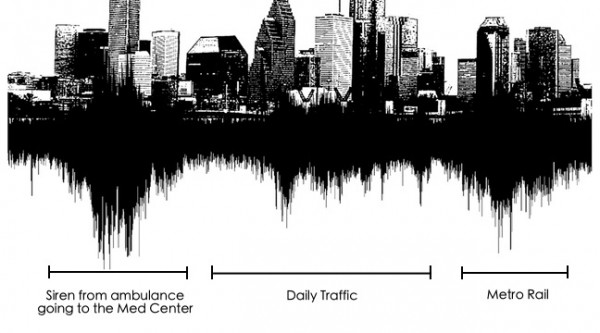
\includegraphics[scale=.5]{gfx/title/citySound.jpg}\footnote{d'après http://www.joesdaily.com/art-design/your-words-turned-into-art/} \\ \medskip
		
		\vfill
		
        \spacedlowsmallcaps{\myName}

        \vfill
        
        \myDegree \\ \bigskip
        
        \myDepartment \\                            
        \myFaculty \\
        \myUni , \myLocation\\ \bigskip
		
		\vfill 
		
        \myTime 

        \vfill                      

    \end{center}  
  \end{addmargin}       
\end{titlepage}   
\thispagestyle{empty}

\hfill

\vfill

\noindent\myName: \textit{\myTitle,} \mySubtitle, %\myDegree, 
\textcopyright\ \myTime

%\bigskip
%
%\noindent\spacedlowsmallcaps{Supervisors}: \\
%\myProf \\
%\myOtherProf \\ 
%\mySupervisor
%
%\medskip
%
%\noindent\spacedlowsmallcaps{Location}: \\
%\myLocation
%
%\medskip
%
%\noindent\spacedlowsmallcaps{Time Frame}: \\
%\myTime

\cleardoublepage%*******************************************************
% Dedication
%*******************************************************
\thispagestyle{empty}
%\phantomsection 
\refstepcounter{dummy}
\pdfbookmark[1]{Dedication}{Dedication}

\vspace*{3cm}

\medskip

\begin{center}
\textit{À ma famille.}
\end{center}
%\cleardoublepage\include{FrontBackmatter/Foreword}
\cleardoublepage%*******************************************************
% Abstract
%*******************************************************
%\renewcommand{\abstractname}{Abstract}
\pdfbookmark[1]{Résumé}{Résumé}
\begingroup
\let\clearpage\relax
\let\cleardoublepage\relax
\let\cleardoublepage\relax

\chapter*{Résumé}

La présente thèse traite de l'analyse de scènes extraites d'environnements sonores, résultat auditif du mélange de sources émettrices distinctes et concomitantes. Ouvrant le champ des sources et des recherches possibles au-delà des domaines plus spécifiques que sont la parole ou la musique, l'environnement sonore est un objet complexe. Son analyse, le processus par lequel le sujet lui donne sens, porte à la fois sur les données perçues et sur le contexte de perception de ces données.

Tant dans le domaine de la perception que de l'apprentissage machine, toute expérience suppose un contrôle fin de l'expérimentateur sur les stimuli proposés. Néanmoins, la nature de l'environnement sonore nécessite de se placer dans un cadre écologique, c'est à dire de recourir à des données réelles, enregistrées, plutôt qu'à des stimuli de synthèse.

Conscient de cette problématique, nous proposons un modèle permettant de simuler, à partir d'enregistrements de sons isolés, des scènes sonores dont nous maîtrisons les propriétés structurelles -- intensité, densité et diversité des sources. Appuyé sur les connaissances disponibles sur le système auditif humain, le modèle envisage la scène sonore comme un objet composite, une somme de sons sources.

Nous investissons à l'aide de cet outil deux champs d'application. Le premier concerne la perception, et la notion d'agrément perçu dans des environnements urbains. L'usage de données simulées nous permet d'apprécier finement l'impact de chaque source sonore sur celui-ci. Le deuxième concerne la détection automatique d'événements sonores et propose une méthodologie d'évaluation des algorithmes mettant à l'épreuve leurs capacités de généralisation.

\newpage

\pdfbookmark[1]{Abstract}{Abstract}
\chapter*{Abstract}

This thesis deals with environmental scene analysis, the auditory result of mixing separate but concurrent emitting sources.  The sound environment is a complex object, which opens the field of possible research beyond the specific areas that are speech or music. For a person to make sense of its sonic environment, the involved process relies on both the perceived data and its context.

For each experiment, one must be, as much as possible, in control of the evaluated stimuli, whether the field of investigation is perception or machine learning. Nevertheless, the sound environment needs to be studied in an ecological framework, using real recordings of sounds as stimuli rather than synthetic pure tones.

We therefore propose a model of sound scenes allowing us to simulate complex sound environments from isolated sound recordings. The high level structural properties of the simulated scenes -- such as the type of sources, their sound levels or the event density -- are set by the experimenter. Based on knowledge of the human auditory system,  the model abstracts the sound environment as a composite object, a sum of sound sources.

The usefulness of the proposed model is assessed on two areas of investigation. The first is related to the soundscape perception issue, where the model is used to propose an innovative experimental protocol to study pleasantness perception of urban soundscape. The second tackles the major issue of evaluation in machine listening, for which we consider simulated data in order to powerfully assess the generalization capacities of automatic sound event detection systems. 

%\newpage
%\chapter*{Résumé Long}
%
%La présente thèse traite de l'analyse des scènes sonores. Par scène sonore, on entend un extrait d'environnement sonore, le résultat auditif du mélange de sources émettrices distinctes et concomitantes. La notion d'environnement ouvre large le champ des sources et des recherches possibles, à la différences des domaines plus spécifiques que sont la parole ou la musique.
%
%L'environnement sonore est un objet complexe. Son analyse, le processus par lequel le sujet lui donne sens, porte à la fois sur les données perçues et sur le contexte de perception de ces données.
%
%Comprendre comment extraire l'information utile de tels objets nécessite donc de se placer dans un cadre écologique, c'est à dire de recourir à des données réelles, enregistrées, plutôt qu'à des stimuli de synthèse, comme des bruits blancs ou des sons purs.
%
%Dans le même temps, que ce soit dans le domaine de la perception ou de l'apprentissage machine, toute expérience suppose un certain contrôle de l'expérimentateur sur les caractéristiques des stimuli proposés. En ce qui concerne les environnements sonores, peu de travaux ont porté sur les outils pouvant permettre aux chercheurs d'agir sur ces stimuli.
%
%Conscient de cette problématique, nous proposons ici un modèle génératif permettant de simuler, à partir d'enregistrements de sons isolés, des scènes sonores dont nous maîtrisons les propriétés structurelles, à savoir, l'intensité, la densité et la diversité des sources sonores en présence. Le modèle envisage la scène sonore comme un objet composite, une somme de sons sources. Le niveau d'abstraction choisi  est motivé par les connaissances disponibles sur le système auditif humain.
%
%Fort des banques de données ainsi constituées, nous investissons deux champs d'application. Le premier concerne la perception, et questionne la notion d'agrément perçu dans des environnements urbains. L'utilisation de données simulés nous permet d'apprécier finement les contributions de chacune des sources sonores dans l'agrément perçu. Le deuxième concerne la détection automatique des événements sonores et propose une méthodologie afin d'évaluer les performances des algorithmes dédiés à cette tâche. Les données simulées se révèlent un outil précieux afin d'évaluer la capacité de généralisation des algorithmes.
%
%Les résultats de nos travaux montrent qu'en générant des scènes sonores artificielles à partir d'enregistrements naturels, d'une manière solidement fondée en théorie, il est possible de dépasser certaines limitations des stimuli synthétiques ou réels, et ainsi d'ouvrir le champ des études sonores à l'usage de données simulées pour l'expérimentation et l'apprentissage. Cette approche s'inscrit dans une tendance de fond pour l'analyse de données complexes, étant la seule à même d'assurer la fiabilité de systèmes fondés sur des algorithmes dont la complexité croissante dépasse aujourd'hui, au même titre que le cerveau humain, nos capacités d'explicitation.

\endgroup			

\vfill
\cleardoublepage%*******************************************************
% Publications
%*******************************************************
\pdfbookmark[1]{Publications}{publications}
\chapter*{Publications}\graffito{\emph{Attention}: This requires a separate run of \texttt{bibtex} for your \texttt{refsection}, \eg, \texttt{ClassicThesis1-blx} for this file. You might also use \texttt{biber} as the backend for \texttt{biblatex}. See also \url{http://tex.stackexchange.com/questions/128196/problem-with-refsection}.}


%\noindent Put your publications from the thesis here. The packages \texttt{multibib} or \texttt{bibtopic} etc. can be used to handle multiple different bibliographies in your document.


\begin{refsection}[ownpubs]

    \small
    \nocite{*} % is local to to the enclosing refsection
    \printbibliography[heading=none]
    
\end{refsection}
\cleardoublepage%*******************************************************
% Acknowledgments
%*******************************************************
\pdfbookmark[1]{Acknowledgments}{acknowledgments}

\medskip

\begingroup
\let\clearpage\relax
\let\cleardoublepage\relax
\let\cleardoublepage\relax
\chapter*{Remerciements}


\endgroup




\pagestyle{scrheadings}
\cleardoublepage%*******************************************************
% Table of Contents
%*******************************************************
%\phantomsection
\refstepcounter{dummy}
\pdfbookmark[1]{\contentsname}{tableofcontents}
\setcounter{tocdepth}{2} % <-- 2 includes up to subsections in the ToC
\setcounter{secnumdepth}{3} % <-- 3 numbers up to subsubsections
\manualmark
\markboth{\spacedlowsmallcaps{\contentsname}}{\spacedlowsmallcaps{\contentsname}}
\tableofcontents 
\automark[section]{chapter}
\renewcommand{\chaptermark}[1]{\markboth{\spacedlowsmallcaps{#1}}{\spacedlowsmallcaps{#1}}}
\renewcommand{\sectionmark}[1]{\markright{\thesection\enspace\spacedlowsmallcaps{#1}}}
%*******************************************************
% List of Figures and of the Tables
%*******************************************************
\clearpage

\begingroup 
    \let\clearpage\relax
    \let\cleardoublepage\relax
    \let\cleardoublepage\relax
    %*******************************************************
    % List of Figures
    %*******************************************************    
    %\phantomsection 
    \refstepcounter{dummy}
    %\addcontentsline{toc}{chapter}{\listfigurename}
    \pdfbookmark[1]{\listfigurename}{lof}
    \listoffigures

    \vspace{8ex}
    \newpage
    %*******************************************************
    % List of Tables
    %*******************************************************
    %\phantomsection 
    \refstepcounter{dummy}
    %\addcontentsline{toc}{chapter}{\listtablename}
    \pdfbookmark[1]{\listtablename}{lot}
    \listoftables
        
    %\vspace{8ex}
%   \newpage
    
    %*******************************************************
    % List of Listings
    %*******************************************************      
    %\phantomsection 
    %\refstepcounter{dummy}
    %%\addcontentsline{toc}{chapter}{\lstlistlistingname}
    %\pdfbookmark[1]{\lstlistlistingname}{lol}
    %\lstlistoflistings 

    %\vspace{8ex}
       
    %*******************************************************
    % Acronyms
    %*******************************************************
    %\phantomsection 
%    \refstepcounter{dummy}
%    \pdfbookmark[1]{Acronyms}{acronyms}
%    \markboth{\spacedlowsmallcaps{Acronyms}}{\spacedlowsmallcaps{Acronyms}}
%    \chapter*{Acronymes}
%    \begin{acronym}[UMLX]
%        \acro{DRY}{Don't Repeat Yourself}
%        \acro{API}{Application Programming Interface}
%        \acro{UML}{Unified Modeling Language}
%    \end{acronym}                     
\endgroup


% Mainmatter
%*******************************************************
\cleardoublepage\pagenumbering{arabic}
%\setcounter{page}{90}
% use \cleardoublepage here to avoid problems with pdfbookmark

\cleardoublepage
\ctparttext{preamble text here.}
\part{Préambule}
%************************************************
\chapter{Introduction}\label{ch:pream_intro}
%************************************************

\jlv{La thèse s'intéresse aux environnements sonores. L'étude se veut pluridisciplinaire, portant à a fois sur l'analyse sensorielle et l'analyse automatique de ces environnements.}
\jls{La présente thèse traite des environnements sonores. L'étude se veut pluridisciplinaire. Elle porte à la fois sur l'analyse sensorielle, et sur l'analyse automatique des environnements.}

\jlv{Par analyse sensorielle, nous entendons l'ensemble des processus qui constituent le système perceptif humain, et lui permettent d'analyser l'environnement qui l'entoure, autrement dit d'en faire sens. Ces processus comprennent à la fois les mécanismes d'acquisition de l'information, et les mécanismes de traitement.} 
\jls{Par analyse sensorielle, on entend l'ensemble des processus qui constituent le système perceptif de l'homme, système par lequel il comprend son environnement, lui donne sens. Ces processus comprennent, d'une part, les mécanismes d'acquisition de l'information, d'autre part, les mécanismes de traitement de l'information.}

\jlv{L'analyse automatique se réfère, quant à elle, au domaine de l'apprentissage machine. L'objectif de ces recherches est d'élaborer des algorithmes permettant à une machine de mimer la perception humaine. Là encore on prend l'habitude de distinguer les étapes d'acquisitions, et de traitement. Les études portant sur l'acquisition de l'information se focalisent sur les descripteurs mathématiques permettant d'extraire une information utile des données brutes du signal. Les études portant sur le traitement se penchent sur les techniques permettant de trier l'information ainsi décrite. Par trie, on entend généralement regrouper les parties de l'information qui se ``\,ressemblent\,''. Ce groupement peut s'opérer soit dans un cadre supervisé, \ie~en considérant une information \emph{a priori} sur la nature des classes d'objets à obtenir, soit dans un cadre non-supervisé, \ie~en effectuant des groupements sur la base seule de l'information à trier.}
\jls{Par analyse automatique on entend l'apprentissage machine. Dans ce domaine, l'objectif des recherches est d'élaborer des algorithmes permettant au "robot" de mimer \jlc{reproduire} la perception humaine. Ici encore on distingue les étapes d'acquisition de l'information, et de traitement de l'information. Les études portant sur l'acquisition se focalisent sur les descripteurs mathématiques permettant d'extraire une information utile des données brutes du signal. Les études portant sur le traitement se penchent sur les techniques permettant de trier l'information ainsi décrite. Trier signifiant regrouper les parties de l'information qui se ``\,ressemblent\,''. Ce tri peut s'opérer soit dans un cadre non-supervisé, \ie~en effectuant les groupements sur la seule base de l'information à collectée, soit dans un cadre supervisé, \ie~en effectuant les groupements sur la base de classes d'objets pré considérées.} \jlc{"sur la base de classes d'objets pré considérées" sur ce coup là je m'avance un peu. Tu peux vérifier?}


\jlv{L'analyse sensorielle a donc trait à la perception humaine, et l'analyse automatique à l'intelligence artificielle. Si ces deux disciplines scientifiques peuvent, de part leurs objectifs et méthodologies différentes, sembler éloignées, elles traitent néanmoins du même problème, à savoir, l'acquisition, la structuration et l'utilisation des connaissances. Ces deux domaines d'études sont les deux faces de la même pièce, \ie~la pensée humaine, la première tentant de comprendre son fonctionnement, et la deuxième de le simuler. À ce titre, elles font toutes deux partie d'un même champ de recherche: les sciences cognitives.} 
\jls{L'analyse sensorielle a donc trait à la perception humaine, l'analyse automatique à l'intelligence artificielle. Les deux domaines peuvent paraître éloignés. Ils portent cependant sur l'acquisition, la structuration et l'utilisation des connaissances, et constituent les deux disciplines d'une même quête, \ie~la pensée humaine, l'une visant à comprendre son fonctionnement, l'autre cherchant à le simuler. À ce titre, perception humaine et intelligence artificielle font toutes deux partie d'un même champ de recherche: les sciences cognitives.}


Les travaux présentés dans cette étude se limitent à une modalité sensorielle particulière, l'audition. Plus particulièrement, elle se focalise sur un type de stimuli: les sons environnementaux. 

Donnons une définition. Habituellement on entend pas son environnemental\footnote{Dans ce document, par souci rédactionnel, nous parlerons indifféremment de son(s) environnemental(aux), d'environnement(s) sonore(s), de scène(s) sonore(s), et de scène(s) sonore(s) environnementale(s), pour désigner les sons environnementaux.} tout extrait sonore qui ne se réclame ni de la parole, ni de la musique. Il s'agit d'une définition par exclusion, musique et parole étant des stimuli étudiés depuis longtemps, bien plus que leur pendant environnementaux. Chacun bénéficie de champs de recherche dédiés, que ce soit en perception\footnote{on parle de perception de la parole (\emph{speech perception}) et de perception de la musique (\emph{music perception})}, ou en intelligence artificielles\footnote{On parle de traitement automatique du langage naturel pour la parole (NLP: \emph{Natural Language Processing}) et de recouvrement de l'information musicale pour la musique (MIR: \emph{Music Information Retrieval})}.

Cette définition \jlc{exit: par la négative} n'est pas satisfaisante. D'un coté, \jlv{elle place les sons environnementaux comme} \jls{elle réduit les sons environnementaux à} des entités secondaires. \jlv{D'un autre coté, l'opposition suggérée entre son environnementaux \vs~sons de paroles et de musiques, deux entités où le sens donné aux sons est de première importance, peut mener à penser que l'influence de la valeur sémantique des sons environnementaux dans leurs traitements est anecdotique, impliquant \emph{de facto} la primauté de leurs caractéristiques physiques} \jls{D'un autre côté, l'opposition suggérée entre sons environnementaux et sons de paroles et/ou de musique, deux domaines où le sens donné aux sons est de première importance, peut mener à penser que l'influence de la valeur sémantique des sons environnementaux est anecdotique, induisant, \emph{de facto}, la primauté de leurs caractéristiques physiques}. Ce qui n'est pas le cas \citep{ballas1987interpreting}. 

Nous prenons dans ce document la définition donnée par \cite{vanderveer1980ecological} (cité par \cite{ballas1987interpreting}).

La définition est en quatre points. Un son environnemental :

\begin{enumerate}
\item est produit par une source réelle;
\item a un sens, en vertu de l'action qui en est la cause;
\item est par essence plus complexe qu'un stimuli de synthèse produit en laboratoire, comme un son pur;
\item ne fait pas partie d'un système de communication.
\end{enumerate} 

Les deux premiers points caractérisent directement les sources émettrices \jlc{exit: des sons environnements}, précisant qu'il s'agit de sources réelles, et insistant sur l'importance du sens qu'elles portent. Nous remarquons cependant que la définition pose la valeur sémantique des sources uniquement par rapport à l'action \jlv{étant la cause le son} \jls{à l'origine du son}. Or l'effet du contexte, et notamment celui relatif à l'individu récepteur, est de première importance: une même scène sonore peut être perçue différemment par deux individus \jlc{exit: différents}. Nous nous proposons ainsi de renforcer le point deux de la définition comme suit:

\begin{itemize}
\setcounter{enumi}{2}
\item a un sens, en vertu de l'action qui en est la cause, ainsi que du contexte d'écoute.
\end{itemize}

Les deux derniers points positionnent les sons environnementaux par rapport aux autres stimuli sonores couramment étudiés, les opposant spécifiquement aux sons de synthèses produits en laboratoire, ainsi qu'aux sons assumant une portée communicationnelle comme la parole ou la musique.

La définition insiste sur le fait que la perception d'un environnement sonore dépend éminemment de l'interprétation sémantique des événements qui la peuplent \jlc{"qui la peuplent" j'aurais dit qui "le" peuplent "le" renvoyant à environnement}, \ie~de l'identification de la nature des sources sonores émettrices. Cette importance de la composition sémantique sur les qualités sensibles des scènes nous permet ainsi d'envisager la scène comme un objet composite, le résultat de l'association des sources sonores qui la constituent.

Partant de cette vision composite des scènes, l'objectif de nos travaux est triple:

\begin{itemize}
\item proposer un modèle morphologique des scènes sonores environnementales, modèle fondé sur une étude approfondie de la littérature ayant trait aux mécanismes régissant la perception des sons environnementaux;
\item montrer l'utilité d'un tel modèle dans le cadre de l'analyse sensorielle;
\item montrer l'utilité d'un tel modèle dans le cadre de l'analyse automatique;
\end{itemize}

Ces objectifs sous-entendent \jls{déterminent} l'organisation de ce document. \jlv{Ce dernier se découpe en quatre parties} \jls{Il comprend 4 parties}. \jlv{La première regroupe le chapitre 1, la présente introduction, et le chapitre 2, qui motive l'approche pluridisciplinaire adoptée dans nos travaux.} \jls{La partie 1 est constituée du chapitre 1, la présente introduction, et du chapitre 2, où est motivée l'approche pluridisciplinaire adoptée dans nos travaux.}

\jlv{La partie 2 traite de l'analyse sensorielle. Elle regroupe trois chapitres.} \jls{La partie 2 traite de l'analyse sensorielle. Elle regroupe les chapitres 3, 4 et 5.} Le chapitre 3 présente un état de l'art des connaissances sur les processus mis en œuvre par le système auditif lors de la perception des environnements sonores. Sur la base de ces considérations perceptives, le chapitre 4 présente un modèle morphologique de scènes sonores environnementales. Il introduit également les outils permettant de simuler, \jlv{à partir modèle proposé} \jls{à partir d'un modèle proposé}, des environnements sonores. Le chapitre 5 présente une série d'expériences montrant comment le modèle introduit permet d'étendre les possibilités des méthodologies classiquement utilisées en analyse sensorielle. Le cadre applicatif choisi par ces expériences est l'évaluation de l'agrément dans les environnements sonores urbains.


\jlv{La partie trois traite de l'analyse automatique des environnements sonores. Elle est composée de trois chapitres.} \jls{La partie 3 traite de l'analyse automatique des environnements sonores. Elle est composée des chapitres 6, 7 et 8.} Le chapitre 6 présente un état de l'art des connaissances sur l'apprentissage machine \jlc{exit: comme} appliqué aux sons environnementaux. Cette présentation s'attache \jlc{s'attache/tâche...} \jls{s'emploie} à détailler les différentes tâches (classification ou détection de sons isolés ou de scènes complexes), les algorithmes couramment utilisés, ainsi que les pratiques expérimentales ayant cours dans ce domaine. Par pratiques expérimentales on entend ici la manière avec laquelle sont évaluées les performances des systèmes proposés, notamment en ce qui concerne les banques de données et les métriques utilisées. Le chapitre 7 précise comment le modèle de scènes sonores proposé peut être appliqué à l'évaluation des algorithmes de détection automatique d'événements sonores. Il montre notamment comment \jlv{ce dernier} \jls{il, ce modèle,...} permet de gagner en connaissance quant à la capacité de généralisation des systèmes de détection proposés. Dans le chapitre 8, nous nous éloignons légèrement du modèle introduit, et proposons un algorithme non-supervisé permettant de recouvrer les similarités existantes entre différentes scènes sonores. Cet algorithme s'appuie sur la vision composite des scènes sonores, en adoptant une approche dite objet. Utilisant une représentation \emph{sparse} du signal, via un descripteur de type \emph{scattering}, l'approche objet groupe, dans un premier temps, \jlv{les éléments d'une même scène étant similaires} \jls{les éléments similaires d'une même scène}. La similarité inter-scène est ensuite calculée sur la base des différents groupes précédemment obtenus. 

\jlv{Enfin, la partie conclusive est composée de deux chapitres: le chapitre 9 qui résume les différentes contributions de cette thèse et conclue quant aux travail effectué. Le chapitre 10 qui discute plus avant à la fois l'approche pluridisciplinaires adoptée et également les résultats obtenus, et propose de nouvelles pistes à explorer.}
\jls{La partie 4, partie conclusive, comprend les chapitres 9 et 10. Le chapitre 9 résume les différentes contributions de cette thèse, et conclue quant au travail effectué. Le chapitre 10, lui, \jlc{"discute plus avant" c'est mal dit. reformuler} à la fois l'approche pluridisciplinaires adoptée et \jlc{exit: également} les résultats obtenus, et propose de nouvelles pistes à explorer.}





 
  
 

%*****************************************
%*****************************************
%*****************************************
%*****************************************
%*****************************************





%************************************************
\chapter{Motivation}\label{ch:pream_motiv}
%************************************************

%*****************************************
%*****************************************
%*****************************************
%*****************************************
%*****************************************






\cleardoublepage
\ctparttext{preamble text here.}
\part{Analyse sensorielle}
%*****************************************
\chapter{La perception de l'environnement sonore}\label{ch:psycho_ea}
%*****************************************

Avant d'aller plus loin dans la présentation de nos recherches, ils nous est indispensable ici de dresser un état des lieux des connaissances liées à la perception des sons.

Nous proposons de présenter ces connaissances en quatre parties. La première récapitule les processus de traitement connus et mises en œuvre à partir du moment où le signal atteint le récepteur, autrement dit le tympan. 

Dans un second temps, nous présentons les résultats émanant de différentes études, regroupées a posteriori sous l'appellation Analyse de Scènes Acoustiques (ASA), et qui s'intéressent à la manière dont le cerveau assimile/ségrègue  les différentes informations contenues dans l'environnement sonore afin d'en dégager des objets cohérents, \ie des sources sonores. 

La troisième partie présente quant à elle les résultats d'études s'attachant a comprendre le fonctionnement  des mécanismes haut niveaux opérant lors de l'évaluation perceptive des environnements sonores, en empruntant une méthodologie issue de la psychologie cognitive. Il s'agit en particulier, d'étudier la contribution, sur l'évaluation globale, des objets composant ces environnements.

Enfin, la dernière partie résume, de manière non exhaustives, ce que le domaine des neurosciences nous apprend sur le traitement de l'information sonore par le cerveau. 

\section{Le traitement de l'information auditive}

\subsection{Perception et cognition}

La perception désigne l'ensemble des processus de traitement de l'information sensorielle. Ces processus nous permettent, par l'interprétation des données reçues en continu par nos organes, de construire une représentation interne du monde qui nous entoure [p. ??]\citep{Houix03f}.

La perception du monde sonore qui nous entoure est un phénomène complexe et encore mal connu. Cette perception est à l'origine de l'interaction que nous créons avec notre environnement. Elle détermine notre capacité d'adaptation à ce dernier. Cette relation au monde \emph{réel} ne se rompt jamais. Nous percevons des sons en permanence, et ce, même si aucune source sonore n'est présente. Ainsi, à la seule lecture d'une partition de musique, le musicien entraînée est capable d'entendre la musique comme si elle était jouée.

Pour la cognition, nous partons d'une définition proposée par U. Neisser \footnote{Ulric Neisser est considéré comme un des pères du cognitivisme notamment grâce à son livre \citep{neisser1967cognitive}. Il a par la suite beaucoup critiqué la direction prise par le mouvement, lui reprochant son recourt excessif aux travaux en laboratoire au détriment des conditions in situ.} dans \citep[p. ??]{neisser1976cognition} .

\begin{quote}
Cognition is the activity of knowing : the acquisition, organisation and use of knowledge.
\end{quote}

Le terme cognition renvoie à la notion de connaissance. Dans un sens plus précis, il désigne les conditions qui permettent l'acquisition et le développement d'une connaissance du monde.

Selon la théorie classique, perception et cognition dépendent de deux groupes de systèmes fonctionnels du cerveau distincts. La perception mobilise les systèmes de traitement dits modaux, c'est à dire supportés par les organes sensoriels (oreilles, yeux etc $\ldots$), tandis que les systèmes cognitifs s'appuient sur des représentations mentales des réalités externes, par essence amodales.

Cette dichotomie entre perception et cognition a été plus récemment critiquée. Dans une approche ``\,incarnée\,'' de la cognition (\emph{Grounded Cognition}), Barsalou nie le caractère amodal des représentations mentales prônant que ces dernières dépendent également des modalités sensorielles \citep{barsalou2010grounded}. Il tente ainsi de réunir les processus perceptifs et cognitifs \citep{goldstone1998reuniting, barsalou1999perceptions}. 

Les deux approches sont illustrées sur la Figure~\ref{fig:processusPercepAndCo}.

\begin{figure}[bth]
        \myfloatalign
        \includegraphics[width=\linewidth]{gfx/Representation}
        \caption{Processus cognitifs et perceptifs}\label{fig:processusPercepAndCo}
\end{figure}

\subsubsection{Psychologie cognitive et psychoacoustique}

La psychologie cognitive est un domaine de recherche dédié aux phénomènes se rapportant à la connaissance. Elle est née dans les années 50, en réaction au \emph{Béhaviorisme}, théorie qui se fonde sur ``\,l'étude des comportements objectivement observables de l'être humain\,'', négligeant, de fait, le rôle de la conscience. La psychologie cognitive, au contraire elle, s'interroge sur des modèles théoriques complexes rendant compte de tous les faits et de toutes les lois connus. Les chercheurs y explorent tout à la fois, la mémoire, le langage, l'intelligence, la perception

L'approche cognitiviste, dans l'étude de la perception auditive, s'éloigne de celle plus traditionnelle de la psychoacoustique \footnote{La psychoacoustique est une branche de la psychophysique qui applique au domaine de l'acoustique les concepts et les méthodes ayant cours en psychophysique.}. Tandis que la psychoacoustique émet l'hypothèse d'une relation directe entre un stimulus et la réponse de l'individu à ce dernier, la psychologie cognitive soutient qu'à un stimulus, l'homme donne des réponses entièrement corrélées au contexte, à l'expérience, aux interactions multi-sensorielles \citep{maffiolo_marieParis_1997}. Ces réponses tiennent compte non seulement des traitements perceptifs mais aussi des représentations issues et de la mémoire individuelle (\ie~construites en particulier à partir de la relation sensible au monde) et de la mémoire collective, à travers le développement des connaissances partagées \citep[p. ??]{maffiolo_caracterisation_1999}.

La psychologie cognitive s'intéresse prioritairement à l'aspect cognitif de la perception en considérant l'individu comme un tout. Elle prend en compte la culture, l'expérience, l'activité de l'individu et ne se focalise pas seulement sur la réaction des organes sensoriels comme l'oreille. Elle questionne les aspects qualitatifs plus que quantitatifs de notre compréhension du monde sonore \citep[p. ??]{maffiolo_caracterisation_1999}.

Elle envisage l'ensemble des étapes du traitement auditif de manière globale et permet ainsi de faire le lien entre une information sensorielle et une information abstraite \citep{mcadams1994penser}.

\subsubsection{Paradigme de la psychologie cognitive}

Comme nous l'avons vu, le cognitivisme ne conçoit pas l'individu comme une ``\,boîte noire\,'', mais envisage ce dernier comme un système de traitement de l'information. Le cognitivisme, fait ainsi l'analogie entre le fonctionnement humain et le fonctionnement de l'ordinateur.

Il ne défend pas l'hypothèse d'un comportement linéaire entre un stimulus externe et la réponse du sujet. Il admet au contraire que le sujet adopte une stratégie, dans le but d'optimiser son comportement face au stimulus. Cette stratégie dépend de la nature du stimulus, du contexte ainsi que des connaissances a priori du sujet.

Maffiolo propose un résumé des présupposés sur lesquels repose le cognitivisme, et qui sont résumés sur la Figure~\ref{fig:paradigmeCognitivisme} \citep[p. ??]{maffiolo_caracterisation_1999} :

\begin{itemize}
\item le monde est discrétisé en dimensions ou propriétés issues de la physique, considérées comme vraies
\item ces dimensions ou propriétés peuvent être mesurées objectivement par des instruments, rendant ainsi compte de la réalité
\item le sujet intègre de manière séquentielle ces dimensions ou propriétés en fonction du contexte
\item l'évaluation subjective du sujet est mesurée comme un décalage par rapport à la mesure objective considérée comme vraie
\end{itemize}

Au regard du paradigme classique de la psychologie cognitive, Maffiolo met en évidence quatre points discutables :

\begin{itemize}
\item la pertinence des dimensions et propriétés physiques utilisées pour le découpage du monde
\item un traitement par les sujets tenant spécifiquement compte de ces dimensions
\item une séparation nette entre stimulus et contexte
\item le caractère subjectif du jugement humain en comparaison à l'objectivité d'un appareil de mesure.
\end{itemize}

\begin{figure}[bth]
        \myfloatalign
        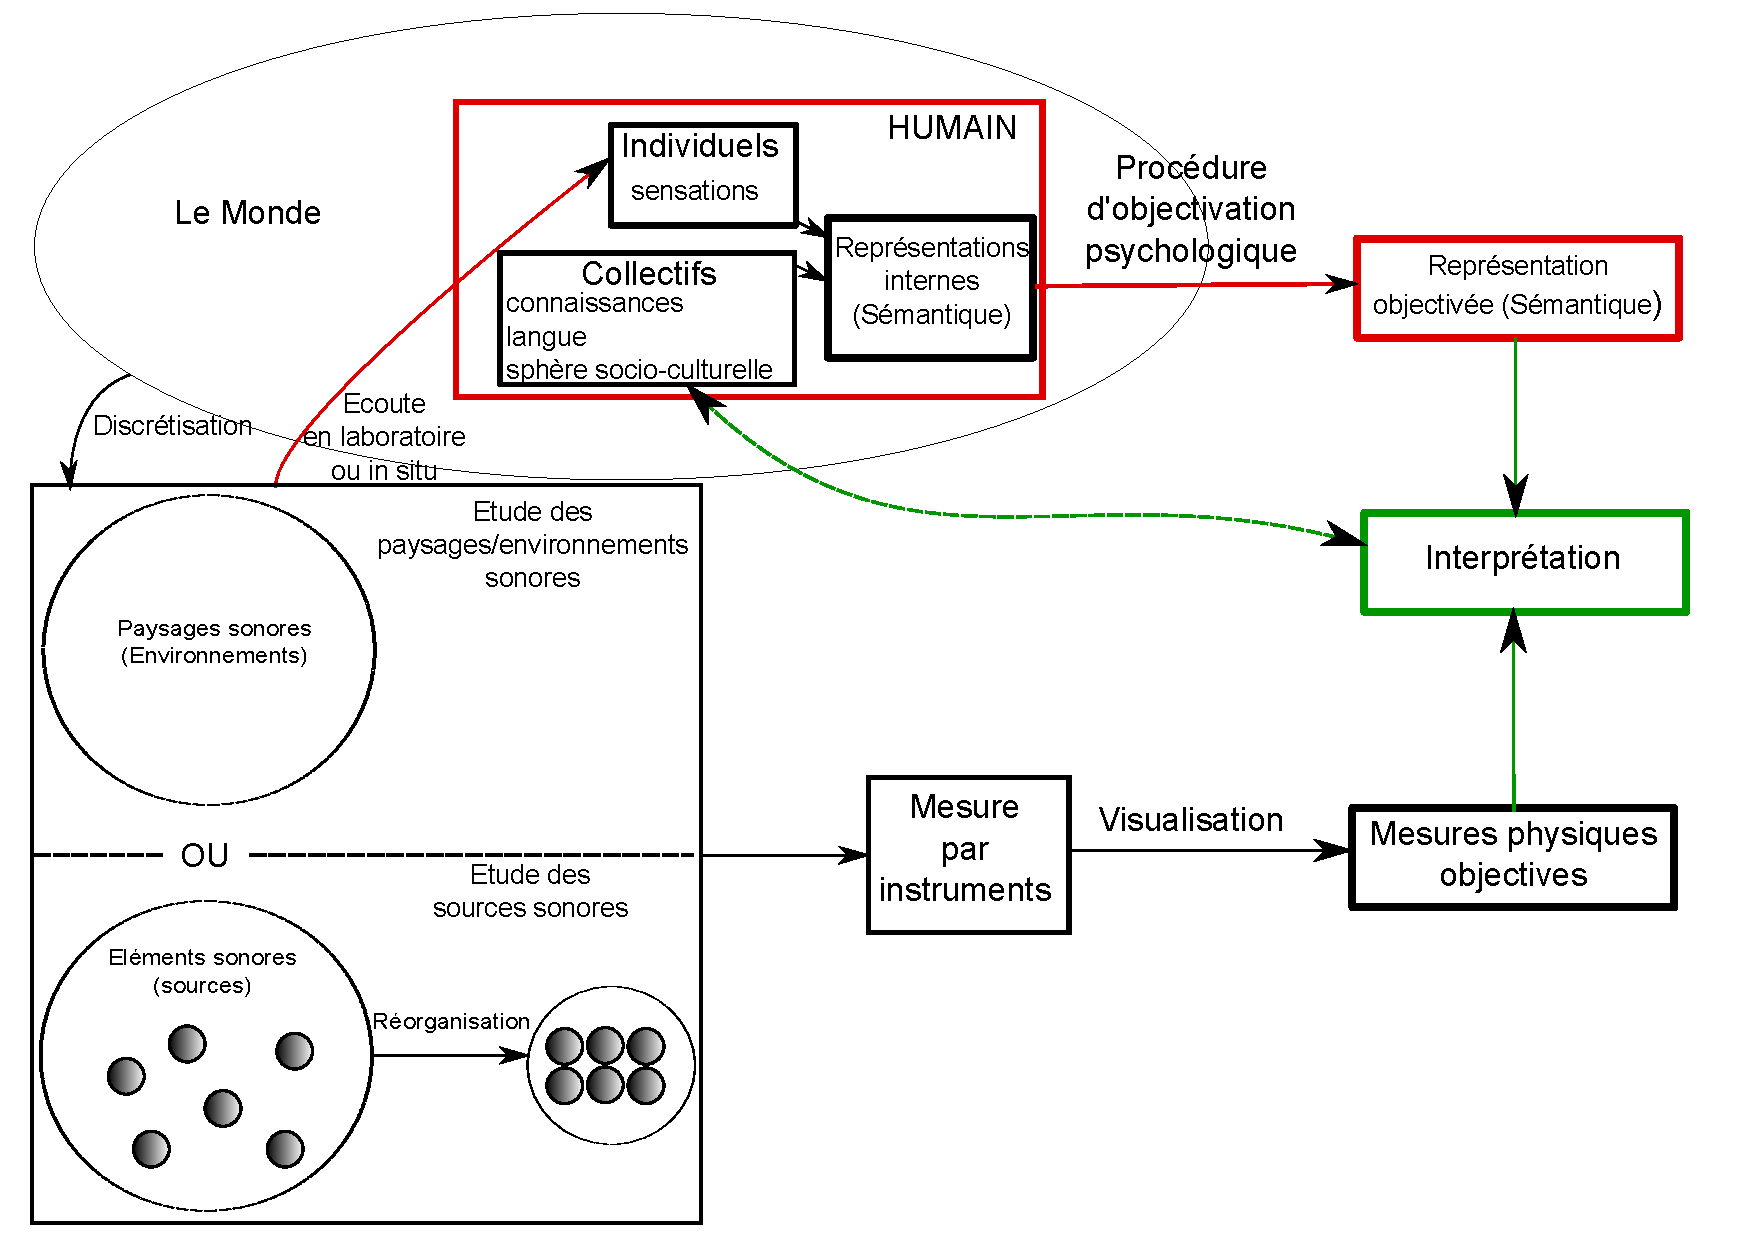
\includegraphics[width=\linewidth]{gfx/Shema_maffiolo}
        \caption[Paradigme du cognitivisme]{Paradigme du cognitivisme, d'après \citep{maffiolo_caracterisation_1999}}\label{fig:paradigmeCognitivisme}
\end{figure}

\subsubsection{L'approche Écologique}
\label{sec:ecologique}

L'approche écologique a d'abord été introduite dans le domaine de la vision par Gibson \citep{gibson1966senses}, qui se demande entre autre si les ``\,lois structurant les objets sont porteuses d'informations, ou si cette information est tirée de comparaison\,'' \citep{gibson1978ecological}.

Cette approche reconnaît que la réponse à un stimulus dépend et de l'information perçue (processus \emph{bottom-up}), et de la connaissance du monde (processus \emph{top-down}), autrement dit l'environnement quotidien et le contexte habituel d'écoute du stimulus.

Afin de garantir une validité écologique, l’approche écologique requiert, dans le cadre d'études perceptives sonores, de prendre en compte cet environnement particulier dans lequel gravitent le sujet et le stimulus. Elle s’oppose ainsi aux méthodes expérimentales traditionnelles, celles de la psychophysique en particulier, en postulant que les expériences en laboratoire décontextualisent le sujet et sa réponse. Une expérience en laboratoire demande en effet au sujet de fournir un effort d'abstraction supplémentaire afin de s’imaginer dans des conditions d'écoute réelle.

A ce titre, un grand nombre d'étude se pratique maintenant dans un cadre \emph{in situ}. On parle d'ailleurs de \emph{soundwalk}  \footnote{\emph{Soundwalk} est un terme anglais introduit par R. Murray Schafer \citep{schafer1969new} signifiant littéralement ``\,marche sonore\,''. Ce terme étant couramment utilisé en français, il ne sera pas traduit dans ce document} pour désigner les expériences où le sujet est immergé dans l'environnement qu'il doit évaluer \citep{adams2008soundwalking,jeon2013soundwalk}.

La méthode des \emph{soundwalk} permet entre autre:

\begin{itemize}
\item  de contextualiser le sujet, à savoir, l'évaluer dans un environnement qu'il connaît et potentiellement qu'il pratique (lieu de vie, de travail)
\item d'évaluer l'environnement sonore, tout en maintenant actif les autres sens (vue, olfaction)
\item de circonvenir aux problèmes de reproduction des environnements sonores en laboratoire
\end{itemize}

Ce problème d'une reproduction écologique des environnements sonores en laboratoire a été particulièrement étudié par Guastavino. \citep{guastavino2003approche,guastavino2004perceptual,guastavino2005ecological}. En comparant les descriptions verbales produites à la suite d'écoutes \emph{in situ} , ainsi que d'écoutes effectuée en laboratoire via des systèmes de reproduction stéréophoniques et multi-phoniques, \citep{guastavino2005ecological} montre que les événements sonores peuplant les scènes sont décrits de la même manière quelque soit le contexte d'écoute. Cependant des différences ont été trouvées concernant la description des fonds sonores (\emph{sound backgrounds}), entre les écoutes stéréophoniques, et les celles multi-phoniques et \emph{in situ}, suggérant de fait que le système de reproduction influe sur les processus cognitifs mis en œuvre. Des conclusions similaires sont faites dans \citep{guastavino2004perceptual} en considérant cette fois-ci des systèmes de reproduction mono, stéréo, et multi-phoniques.

Cependant, les études \emph{in situ}, bien qu'étant écologiquement plus valides que des études en laboratoire, présentent elles aussi des inconvénients. Dans le cas où tous les sujets ne passent pas l'expérience au même moment, il est impossible de garantir qu'ils soient soumis aux mêmes stimuli. De facto, la reproductibilité des expériences est elle aussi plus difficile. A l'inverse, le cas où l'expérience est passée de manière simultanée par tous les sujets peut faire émerger des problèmes pratiques d'organisation, notamment en ce qui concerne le maintien du sujet dans une attitude propice à passer une expérience.

\subsection{L'écoute}

\subsection{Le chaîne traitement de l'information auditive}
\label{sec:chaineTaite}

Le son est une vibration émise par une source d'excitation, et transmise à l'air. Cette vibration se propage ensuite jusqu'à atteindre un récepteur, le tympan, qui va capter le différentiel de pression résultant de cette vibration. C'est le point de départ du processus de traitement de l'information auditive. 

Si on adopte une approche \emph{traitement de l'information}, on peut décomposer ce processus en plusieurs systèmes inter-connectés. Ces systèmes forment une chaîne qui, au fur et à mesure des traitements, interprète le signal acoustique afin d'en extraire l'information sémantique. Plus on se place loin dans la chaîne de traitement, plus on a accès à une information abstraite, potentiellement utilisable par d'autres processus de haut niveau. La figure \ref{fig:traitementSonMcAdamsBigand} extraite de \citep{mcadams1994penser} nous donne un aperçu des principales fonctionnalités du système de traitement auditif.

\begin{figure}[bth]
        \myfloatalign
        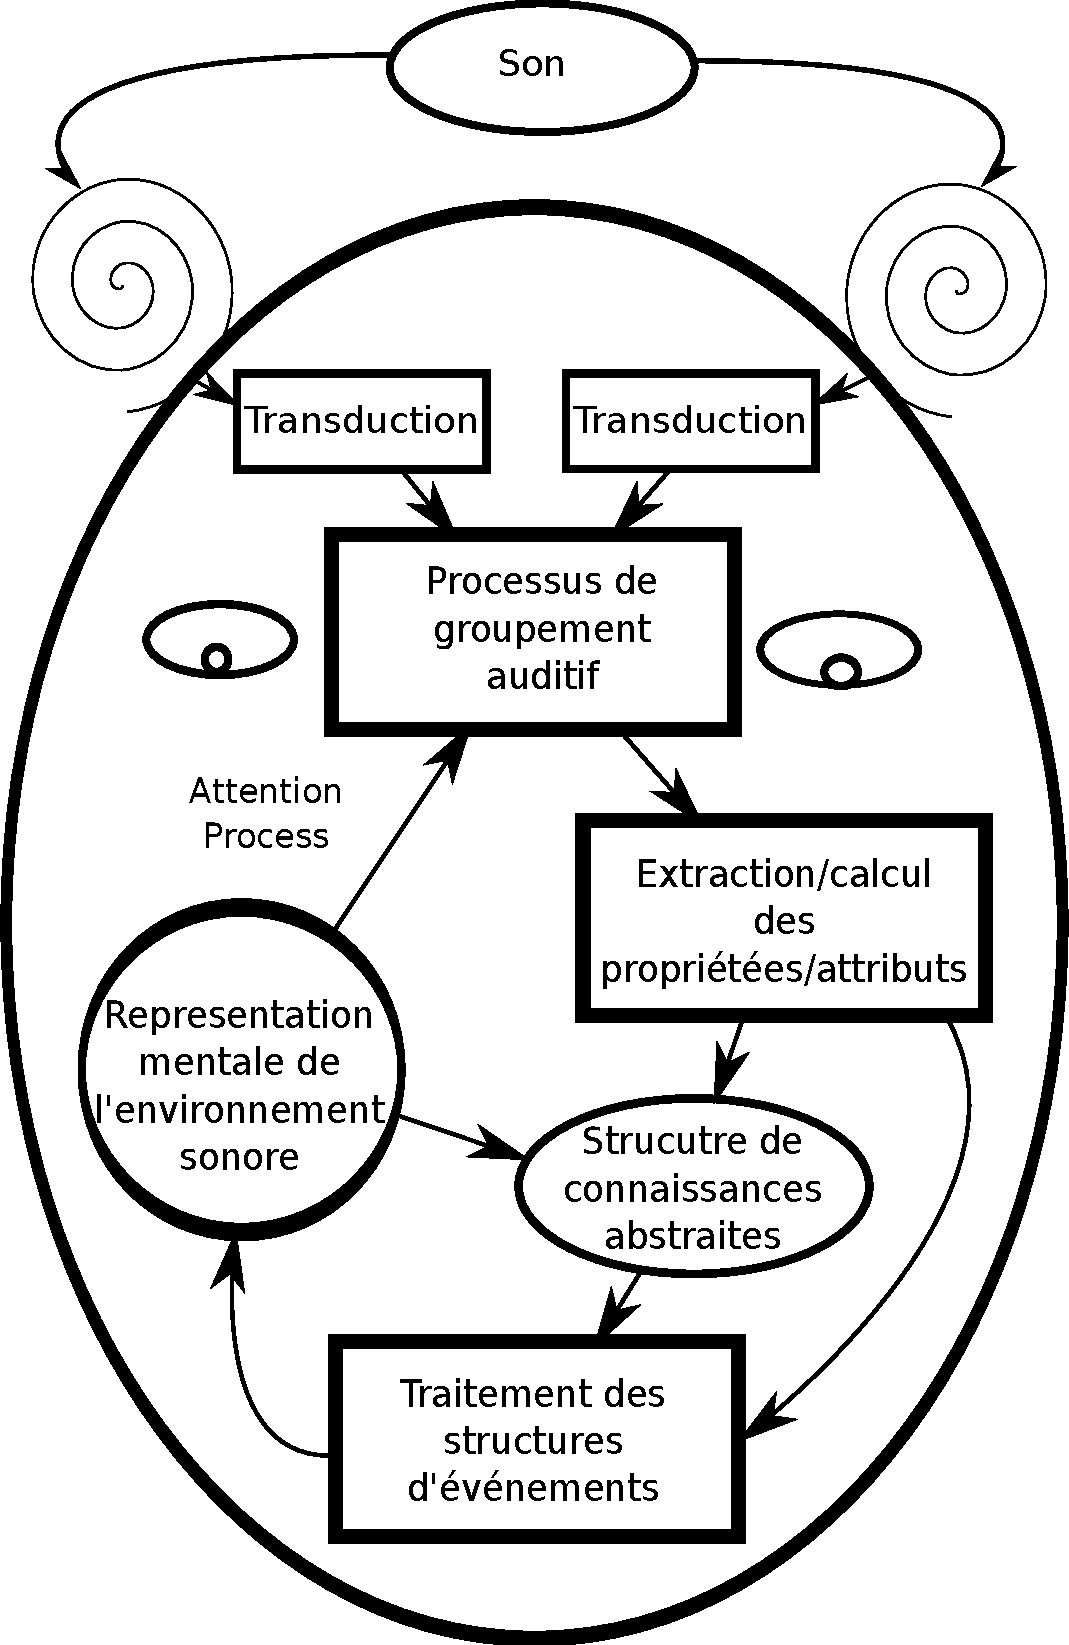
\includegraphics[width=.6\linewidth]{gfx/traitementSonMcAdamsBigand}
        \caption[Principaux processus de traitement de l'information auditive et leurs interactions]{Principaux processus de traitement de l'information auditive et leurs interactions, à partir de \citep{mcadams1994penser}}\label{fig:traitementSonMcAdamsBigand}
\end{figure}

Lors de l'étape de \emph{transduction}, les vibrations sonores parvenant au tympan sont analysées puis traduites en impulsions nerveuses transmises au cerveau. Ces impulsions rendent compte des attributs spectraux et temporels de l'onde. L'extraction des composantes fréquentielles intervient dans la cochlée. C'est à l'intérieur de cette dernière que les différentes parties de la membrane basilaire vont être excitées en fonction des fréquences composant le signal, suivant un axe tonotopique. Les vibrations captées à chaque point d’excitation de la membrane basilaire sont transmises au cerveau via les nerfs auditifs, chaque point codant une information correspondant à une bande fréquentielle limitée. 

Vient ensuite le \emph{processus de groupement auditif}. C'est une étape d'intégration temporelle au cours de laquelle l'information est analysée en images auditives cohérentes. Contrairement à ce que pensaient les Grecs, nous ne possédons pas de "canaux" séparés pour chaque objet sonore présent dans l'environnement \citep{yost1994fundamentals}. C'est notre cerveau qui se charge de fusionner et de discrétiser les éléments sonores simultanés afin de créer un flux auditif structuré. En d'autres termes il s'agit de déterminer, combien d'objets sonores sont présents, d'où viennent t-ils et quel est leur sens. Les recherches regroupées sous l'appellation ``\,analyse de scènes auditives\,'', abordées à la section~\ref{sec:ASA} ont  extensivement étudié ces processus de groupement.

Prenons pour exemple les chorals de Bach. C'est le \emph{processus de groupement auditif} qui nous permet, sur la base des paramètres spectro-temporels du signal, de distinguer les quatre voix basse, ténor, alto et soprano. Par contre c'est à partir d'une analyse des attributs perceptifs que nous sommes capables de percevoir les mélodies comme des objets unitaires, même si ces dernières sont développées entre les différentes voix du choral. Cette extraction des propriétés perceptives intervient pendant la phase dite \emph{d'extraction/calcul des propriétés/attributs}.

Une définition des représentations mentales est donnée par \citep{houde1998vocabulaire}:

\begin{quote}
``\,La représentation mentale peut être vue comme une entité interne, le correspondant cognitif individuel des réalités externes expérimentées par un sujet.\,''
\end{quote}

Ces représentations font office de sauvegardes de l'information. Conservées en mémoire sous une forme hautement abstraite \citep[p. ??]{mcadams1994penser}, elles rendent compte à la fois de notre compréhension du monde et de la manière dont nous l'abordons. Ces connaissances subjectives, non directement observables, restent néanmoins accessibles au chercheur par le biais d'expériences d'objectivation (voir section~\ref{sec:appCategorielle})

\subsection{Processus Bottum-up et processus Top-down}

L'interaction entre l'homme et son environnement est fonction d'une part de l'information sensorielle captée par le sujet, d'autre part de la rétroaction exercée par lui sur ces données. Cette rétroaction est déterminée par son expérience sensible du monde. Par "expérience sensible", nous entendons la mémoire interne des interactions passées, mémoire grâce à laquelle nous optimisons l'analyse des stimuli, et intégrons les effets de contexte dus à l'environnement.

Cette mémoire est à la fois :

\begin{itemize}
\item individuelle : dépendant de notre expérience propre
\item collective : dépendant des connaissances que nous avons acquises sur le monde
\end{itemize}

La rétroaction est l'expression de l'individualité du sujet, individualité qui explique que deux personnes ayant des capacités sensorielles semblables peuvent percevoir différemment un même environnement.

Ainsi la perception mobilise deux formes de traitements :

\begin{itemize}
\item les traitements dits ascendants (bottom-up) dirigés par les données
\item les traitements dits descendants (top-down) dirigés par les concepts ou les représentations
\end{itemize}

Étudier la perception demande de prendre en compte aussi bien l'information externe (processus ascendant) que l'information interne (processus descendant). Réduire la perception à une simple association de sensations ne permet pas de rendre compte de l'éventail des processus cognitifs entrant dans le décodage de l'environnement. Un exemple parlant concret, emprunté au domaine de la vision, est celui du phénomène dit de bi-stabilité, \ie~La faculté, chez un sujet, de voir dans une même image tantôt un canard, tantôt un lapin, autrement dit, de tirer d'un même stimulus deux analyses différentes, mais jamais simultanément (\Cf~Figure\ref{fig:bistabilite}).

Un autre exemple, cette fois dans le domaine de l'audition, nous semble illustrer le caractère dual de la perception. Il est donné par McAdams et Bigand \citep[p. 2]{mcadams1994penser}:

\begin{quote}
``\,...Imaginez vous un instant en pleine forêt amazonienne : vous entendriez exactement les mêmes bruits que le guide qui vous accompagne, mais, étant donné votre manque de connaissance du milieu, vous seriez incapable d'extraire du fond sonore les sons correspondant aux cris de l'iguane, aux singes macaques, aux chants des ouistitis ou aux bruissements des arbres tropicaux. De ce fait vous seriez dans l'incapacité d'attribuer une signification à l'ensemble de la structure sonore, ce qui pourrait être important pour votre survie dans l'environnement.\,''
\end{quote}

\begin{figure}[bth]
        \myfloatalign
        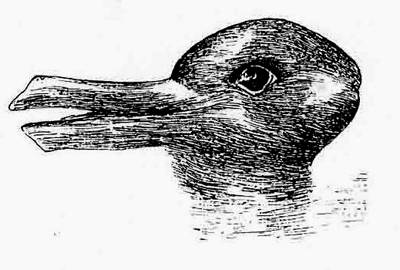
\includegraphics[width=.6\linewidth]{gfx/canard_lapin}
        \caption[Le phénomène de bistabilité: l'illusion du canard-lapin]{Le phénomène de bistabilité: l'illusion du canard-lapin. Première publication dans \emph{Fliegende Blätter}, 23 octobre 1892, p. 147}\label{fig:bistabilite}
\end{figure}

En psychologie cognitive, on distingue ainsi les approches cognitivistes, qui s'intéressent plus particulièrement aux processus de type \emph{botttom-up} relatifs au traitement de l'information perçue , des approches dites cognitives, lesquelles interrogent, avant tout, les processus de type \emph{top-down} liés à la mémoire du sujet ainsi qu'au contexte \citep[p. ??]{guastavino_etude_2003}.

\section{Représentation mentale de l'environnement sonore}
\gl{Cette partie (Représentation de l'environnement sonore) devra être réorganisée. s'appuyer sur \citep{Houix03f} et \citep{goldstone2003concepts}. Ne pas corriger}

Les représentations forment une image mentale discrète d'un monde physique continue \citep{houde1998vocabulaire}. C'est par ce passage du continu au discret que nous sommes à même d'organiser nos connaissances, afin de les réutiliser de manière efficace. Les objets discrets qui forment cette organisation sont appelés des catégories. L'action consistant à juger si un événements perçu appartient à une catégorie, est elle appelée la catégorisation.

\subsection{Théorie de la catégorisation}

Nous considérons ici le processus de catégorisation comme initialement formalisée par E. Rosch et B. B. Lloyd \citep{rosch1978cognition}, et nommée théorie prototypique de la catégorisation. Il est à noter que l'étude de la catégorisation est antérieure aux travaux de Rosch, et que depuis, d'autres proposition ont été faite afin d'étendre la théories prototypique, comme la théories des exemplaires ou \textit{context theory} \citep{medin1978context}, et son extension multidimensionnelle \citep{medin1978context}. Mais les travaux de Rosch étant à l'origine de ces théories postérieures, nous nous appuierons sur ces derniers afin de détailler de manière générale le fonctionnement des processus de catégorisation. 

Un des principes essentiel de tout être vivant est de segmenter son environnement, \ie~de se bâtir un système de classification permettant de regrouper des objets n'étant pas identiques \citep[p. 1]{rosch1978cognition}. On appelle catégorisation, l'action consistant à regrouper des objets du monde physique considérés comme équivalents, et catégorie, l'objet mental contenant le groupe d'objets ainsi rassemblé. 

Il est important de noter qu'à chaque catégorie est associé un label, censé décrire du mieux possible l'ensemble des objets inclus dans la catégorie. On parlera alors de catégories sémantiques. L'ensemble des catégories sémantiques conservées en mémoire forment la représentation mentale qu'un individu se fait du monde, des réalités externes. 

L'introduction de cette dimension sémantique a des conséquences importantes sur l'universalité présupposée de la catégorisation. Cette dernière étant codée par la langue, elle ne dépend plus seulement d'une réalité physique, mais également d'un contexte culturel. La catégorisation peut être vue comme un action intermédiaire entre, d'une part l'organisation d'une connaissance individuelle résultant d'une expérience sensorielle personnelle, et la constitution d'une représentation collective pouvant être partagée par le biais d'un langage commun \citep{dubois2006cognitive}. 

Selon Rosch, la catégorisation obéit à deux principes \citep[p. 29]{rosch1978cognition}:

\begin{enumerate}
\item \textit{L'économie cognitive}: la catégorisation doit fournir un maximum d'information pour un minimum d'effort. La structure du système catégoriel s'élabore en tenant compte de se principe d'économie. On comprend alors que la catégorisation d'un objet est soumise à un contexte sensoriel, c'est à dire aux autres objets perçus simultanément, et qui doivent être eux aussi catégorisés. Comme énoncé par D. Dubois \citep[p. 33]{dubois1991semantique}:
\begin{quote}
``\,Catégoriser un stimulus signifie le considérer dans la finalité de cette catégorisation, non seulement comme équivalent des autres stimuli de la même catégorie, mais également différent des stimuli qui n'appartiennent pas à cette catégorie\,''.
\end{quote}

Il apparaît clairement que la catégorisation d'un objet ne se veut pas absolue, autrement dit, l'appartenance d'un objet à une catégorie ne dépend pas uniquement de l'observation d'une propriété particulière, mais également du contexte dans lequel cette objet est perçu.

\item \textit{La redondance structurelle}: l'ensemble des objets physiques ne vie pas dans un espace aux dimensions bien identifiées, finies, et dont les valeurs seraient équiprobables. En d'autres termes, le monde ne peut se réduire à des paramètres dimensionnés, indépendants et manipulables, comme dans le cadre d'études en laboratoire. Au contraire, il peut exister des discontinuités saillantes entres objets, de même que ces objets sont souvent liés entre eux par des patterns de co-occurrence de propriétés (exemple : un chien possède "quatre pattes et un museau" plus souvent que "deux pattes et un museau"). Ces discontinuités et corrélations, présentes dans les propriétés perçues, étayent la structure catégorielle de notre représentation mentale,  et gouvernent ainsi le processus de catégorisation.
\end{enumerate} 

Rosch propose de voir la structure catégorielle suivant deux axes:

\begin{itemize}
\item \textit{axe vertical}: Il s'agit de l'organisation hiérarchique des catégories, qui illustre la manière dont les catégories sont incluses les unes dans les autres. Cette dimension verticale peut être vue comme une taxonomie, les catégories de haut-niveaux représentant des objets abstraits ou concepts, et incluant un grand nombre de sous catégories, et les catégories de bas-niveaux représentant des objets concrets, incluant peut de sous catégories. Ainsi, plus le niveau d'abstraction est grand, plus les similitudes entre objets d'une même catégorie (intra-catégorielle), ainsi que la similitude entre objets de catégories distinctes (inter-catégorielle) son faibles. Inversement, plus le niveau d'abstraction est faible, plus les similitudes intra- et inter-catégorielle sont élevées. Rosch propose de décomposer cette dimension verticale en trois niveaux d'abstraction (\Cf~Figure~\ref{fig:categorieLVL}): Superordonné, Base et subordonné. Le niveau superordonné représente les catégories avec un haut niveau d'abstraction tandis que le niveau subordonné représente les catégories concrètes. On voit bien que les périmètres définis par les catégories du niveaux superordonnées (Mobilier, Véhicule) sont larges, \ie~les objets contenus dans ces catégories peuvent être très distincts. A contrario, les catégories du niveaux subordonnées (chaise longue, cabriolet) sont très précises, et les objets qu'elles contiennent très similaires entres eux. Cependant, on notera que les objets de la classe Cabriolet ont potentiellement beaucoup de propriétés en commun avec les objets de la classe Berline (par exemple), beaucoup plus que celles que partagées entre les objets des classes Mobilier et Véhicule. 
\item \textit{axe horizontal}: Cette dimension peut être vue de deux manières: 1) elle illustre la manière dont sont séparées des catégories partageant le même niveau d'abstraction, 2) elle permet d'apprécier le degré de typicité des différents objets appartenant à une même catégorie. En effet, les catégories ne sont pas des objets discrets, car les propriétés attribuées aux objets qu'elles contiennent peuvent être partagés par d'autres catégories. Ainsi, les frontières entre les différentes catégories ne sont pas figées et peuvent se recouvrir. Pour discriminer les catégories, Rosch propose de ne pas raisonner en terme de frontières, mais plutôt de décrire chaque catégorie par un nombre de cas non ambiguës (clear case) \citep[p. 36]{rosch1978cognition}. Tous les objets d'une catégorie ne sont pas également représentatifs de cette dernière, les cas non ambiguës peuvent être vus comme les objets les plus typiques de la catégorie. Ce fait est empirique, il a été montré que des sujets peuvent très bien s'accorder sur la typicité d'un objet par rapport à une catégorie, tout en n'étant pas d'accord sur les frontières de cette dernière \citep{rosch1974human,rosch1975cognitive}. Le terme prototype, qui donne son nom à la théorie, vient de l'hypothèse que, parmi ces cas non ambiguës, il en existe un, le prototype, plus représentatif que les autres, et qui forme le noyau de la catégorie.
\end{itemize}

\begin{figure}[bth]
        \myfloatalign
        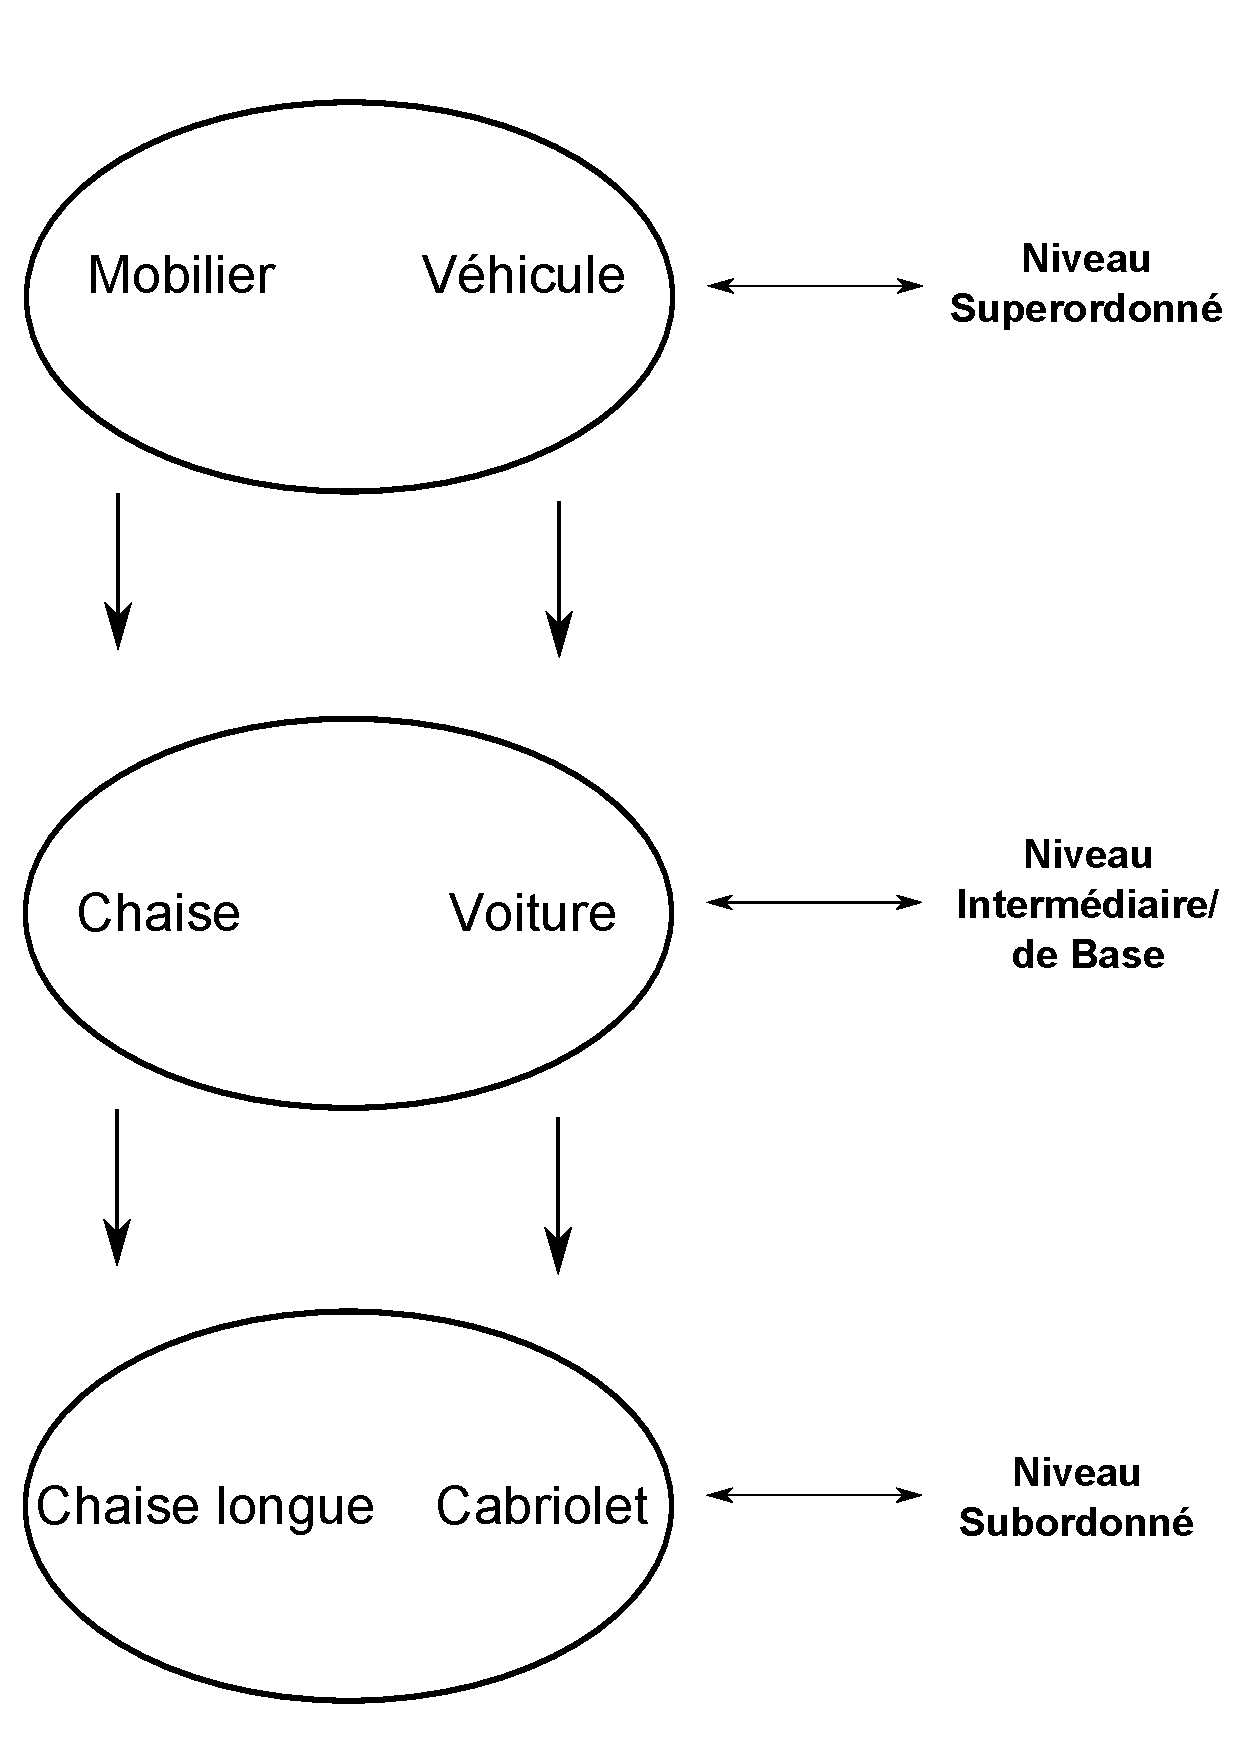
\includegraphics[width=.6\linewidth]{gfx/categorieLVL}
        \caption{Les trois niveaux d'abstraction de l'axe vertical de la structure catégorielle.}\label{fig:categorieLVL}
\end{figure}

Les catégories sont structurées en interne, en référence à un prototype, \ie~l'objet possédant les attributs typiques de celle-ci. L'appartenance d'un objet à une catégorie dépend alors de la ressemblance qu'entretient ce dernier avec le prototype.  Plusieurs proposition ont été faites afin de définir le prototype d'une catégorie: Pour Tversky \citep{tversky1977features}, le membre prototype sont celui dont la somme des similarités avec les autres membres de la catégorie est la plus grande. Pour \citep{rosch1975family}, il s'agit de l'objet possédant le plus de propriétés en commun avec les objets de la catégorie, et le moins de propriétés avec les objets des catégories externes. Dans ce cas, la typicité d'un élément d'une catégorie est donc fonction de son degré d'appartenance à celle-ci, ainsi que de son indépendance vis à vis des autres catégories. En se limitant à l'observation d'attributs vivant dans un espace métrique, \citep{reed1972pattern, rosch1976structural} ont montré que le prototype est un centroid, un objet définit comme étant la moyenne des attributs des objets de la catégories.

Mais il faut bien comprendre que cette théorie prototypique de la catégorisation, bien que se basant sur des faits expérimentaux, est avant tout une vision pratique, un concept qui n'a pas été clairement défini et dont l'implication dans les processus de catégorisation reste floue \citep[p. 36-40]{rosch1978cognition} \citep[p. 49-54]{dubois1991semantique}.

\section{Analyse de scènes acoustiques}
\label{sec:ASA}

\subsection{Définition}
\label{sec:ASAintro}

L'analyse de scène est un terme d'abord introduit de la cadre des recherches informatiques en vision. Il fait référence aux différentes stratégies par laquelle un ordinateur parvient à isoler un objet d'une image~\citep[p. 12]{mcadams1994penser}. Le pendant acoustique de l'analyse scène, est nommé l'Analyse de Scène Acoustique (ASA). Le terme ASA a été introduit par Albert S. Bregman dans son ouvrage de référence \citep{bregman1994auditory}.  

L'ASA désigne l'ensemble des processus perceptifs permettant d'isoler d'une mixture sonore \footnote{On entend par mixture sonore, ou magma sonore, un ensemble de sons provenant de différentes sources sonores}, les informations émanant d'une source sonore distincte, et à les regrouper afin de les traiter comme un tout cohérent.  L'ASA part en effet du principe que, afin de faire sens de l'environnement qui l'entour, il est nécessaire pour le cerveau d'isoler les informations relatives aux différentes sources sonores \citep{winkler2009modeling}. On parle alors indifféremment de processus de ségrégation ou de groupement.

La définition de l'ASA est très large. Comme vu dans la section~\ref{sec:chaineTaite}, les processus de groupement sont composés à la fois de processus \emph{bottum-up}, \ie~ dirigés par l'information auditive transduite (représentation temps-fréquence du signal sonore), ainsi que de processus \emph{top-down} dirigés par les connaissances stockées en mémoire. Dans la théorie de l'ASA, les processus \emph{bottum-up} sont appelés \emph{processus primitifs}, et les processus  \emph{top-down}, \emph{processus basés sur des schémas}. 

Pour les premiers, il s'agit de systèmes de traitement innés, opérant sur la base de régularités présentes dans le signal, afin de regrouper les composantes fréquentielles produites par une même source. Par régularité on comprend ici des propriétés constantes de l'environnement, perçues par l'ensemble des êtres humains, partout sur la planète. Par exemple, si la fréquence fondamentale d'un son harmonique change au cours du temps, toutes ses harmoniques changeront également afin de maintenir la structure harmonique du son [p. 38]\citep{bregman1994auditory}. Les \emph{processus basés sur des schémas}  partent eux de schémas, \ie~connaissances apprises formant notre représentation mentale du monde, formés par le biais d'écoutes antérieures. 

La plupart des recherches sur l'ASA adopte encore maintenant une approche cognitive, en se concentrant sur l'étude des \emph{processus primitifs}. Cependant, elles suivent généralement une méthodologie expérimentale très inspirée de la psychoacoustique.

\subsection{Une approche psychoacoustique}

L'étude de l'ASA adopte une méthodologie s'inspirant largement du paradigme de la psychoacoustique. Ainsi les réponses du sujets sont évaluées par rapport à un stimuli décrit analytiquement dans un espace multidimensionnel de dimensions physiques (fréquence, intensité etc $\ldots$) \citep{dubois2006cognitive}. Dans la grande majorité des cas, les stimuli utilisés sont des sons pures ou complexes\footnote{Par son pur on entend un son composé d'une seule sinusoïde, \ie~possédant une seule fréquence. A contrario, un son complexe est un son composé de plusieurs composantes fréquentielles}, bien évidemment synthétisés en laboratoire. 

Ces sons sont alors proposés à l'écoute à un sujet, de manière séquentielle. Il s'agit alors, au cours de la séquence, de faire varier un paramètre (intensité, hauteur fréquentielle, espacement entre les séquences), et d'observer le seuil à partir duquel ce changement a un effet significatif sur la capacité du sujet à distinguer plusieurs sources sonores.

L'étude de l'ASA se restreint donc à l'analyse de l'effet de descripteurs bas niveaux sur les processus d'intégrations, sans tenir compte d'attributs perceptifs plus haut niveaux, comme la valeur sémantique attribuée aux sons, ni de considérations écologiques~\ref{sec:ecologique}. En conséquence, il est parfois difficile de faire le lien entre la notion de source sonore comme utilisée dans les études psychoacoustique de l'ASA, et celle adoptée par les études en psychologie cognitive. En théorie, pour les deux approches, le terme source sonore se réfère directement à l'objet (\eg~voiture) supposé être la source d'émission d'un son réel. En psychologie cognitive, cette relation est directe, le stimuli étant la plupart du temps un enregistrement de ladite source. En psychoacoustique, la relation directe est difficile, les stimuli étant des sons de synthèses, inexistant dans le monde réel. La source sonore désigne alors plutôt un objet abstrait, dont l’existence est avérée à partir du moment ou un agglomérat de sinusoïdes est interprété par le sujet comme étant un tout, émanant de facto d'une seule entité. 

Il s'agit là d'une des limitations de l'approche psychoacoustique appliquées aux études des  \emph{processus primitifs} de l'ASA. Les résultats, obtenus à partir de stimuli très éloignés de la réalité des phénomènes acoustiques perçus, étant difficiles à généraliser à des applications plus incarnés.

\subsection{Régularités et processus primitifs}

L'existence des \emph{processus primitifs} est une conséquence de la présence dans le monde sonore de régularités universelles affectant l'ensemble des stimuli auditifs. Bregman distingue 4 types de régularités [p. 19,21,31,33]\citep{mcadams1994penser}:

\begin{enumerate}
\item \emph{Synchronicité}: Il est rare que des sons n'ayant aucun rapport entre eux démarrent et s'arrêtent au même moment.
\item \emph{Continuité}: 
\begin{itemize}
\item Les propriétés d'un son isolé tendent à se modifier lentement et de façon continue.
\item Les propriétés d'une séquence de sons émis par la même source tendent à se modifier lentement.
\end{itemize}
\item \emph{Harmonicité}: Lorsqu'un corps sonore vibre à une période répétée, ses vibrations donnent naissance à un pattern acoustique dont les fréquences des composants sont des multiples d'une même fréquence fondamentale
\item \emph{Uniformité}: La plupart des modifications qui surviennent dans un signal acoustique affectent tous les composants du son résultant, de manière identique et simultanée.
\end{enumerate}

Notre perception du monde est contrainte par la présence de ces régularités. A ce titre, les \emph{processus primitifs} sont des systèmes perceptifs innés, uniquement dépendant des stimuli. On peut les voir comme une série de règles génériques qui nous permettent, sur la base des régularités, d'isoler du monde sonore des objets cohérents \citep{ballas1987interpreting}. Il s'avère que ces règles sont très proches de celles opérant pour la perception des formes dans le cadre de la vision.  

\subsection{Perception de la forme}

Que ce soit en vision ou en audition, notre cerveau est en permanence stimulé un ensemble de sources distinctes. Percevoir un objet dans cet agglomérat, c'est être capable d'isoler tous les signaux émis par une même source, et de les réunir en une unité perceptive cohérente.

Parmi les premiers travaux qui se sont intéressés à ces processus de groupement, on trouve la psychologie de la forme, ou plus communément appelée \emph{Gestalt Theory} (\emph{Gestalt} étant un mot allemand pouvant être traduit par forme). Cette théorie, introduite par Ernst Mach et Christian von Ehrenfels à la fin du XIXème siècle, se propose d'expliciter les principes selon lesquels des stimuli sensoriels sont combinés afin de former un pattern mental rendant compte de la présence d'un objet présent dans l'environnement. 

Ces principes ont principalement été établis en considérant le problème de la perception visuelle. Mais il a depuis été montré qu'ils restent vrais dans le cadre de la perception auditive \citep[ch. 1]{bregman1994auditory}. Parmi ces principes, nous en détaillons cinq:

\begin{enumerate}
\item \emph{Proximité}: Des éléments proches les uns des autres ont tendance à être groupés ensembles. En audition, ce principe de proximité opère suivant les différentes caractéristiques du sons, à savoir, la fréquence, l’onset \footnote{En traitement du signal audio, on désigne par le mot anglais onset le début du signal. Ce terme étant couramment utilisé en français, nous ne le traduirons pas dans ce document.} et l'intensité. 
\item \emph{Similarité}: Des éléments qui se ressemblent ont tendance à être groupés ensembles.
Dans le domaine de la vision, la proximité est réservée au domaine spatial, alors que la similarité est réservée aux caractéristiques physiques de l'objet (forme, couleur, etc $\ldots$), qui ne peuvent se décrire suivant une unique dimension. De même en audition, on parlera de manière générale de proximité temporelle (onsets proches) et non de similarité. Pour le reste des descripteurs utilisé en audition, il est cependant difficile de clairement distinguer les principes de proximité et de similarité. Bregman propose de réserver le terme proximité lorsque l'on considère une dimension physique particulière, et d'utiliser le terme similarité lorsque l'on considère un ensemble de descripteurs, ou lorsque l'on traite d'attributs qui ne peuvent être clairement décomposés suivant des dimensions distinctes, comme le timbre.
\item \emph{Continuité}: Des éléments qui varient de manière non abrupte ont tendance à être groupés ensembles. Par ce principe, des objets distincts mais proches temporellement (respectivement spatialement pour la vision) ont tendance à être perçus comme le prolongement des uns par rapport aux autres. A contrario, une changement abrupte indique généralement l'apparition d'une nouvelle source. C'est ce principe qui nous permet de percevoir comme une seule entité, un objet dont les caractéristiques varient dans le temps,\eg~le son d'une sirène.
De récentes études en neurosciences ont montré l'importance de ce principe dans les processus de groupement. Notamment\citep{winkler2009modeling} qui proposent de voir l'ASA comme un processus prédictif, le cerveau cherchant à anticiper la nature des stimuli qui lui parviennent, sur la base de régularités extraites des objets détectés dans l'instant précédant.
\item \emph{Clôture}: Des éléments discontinus qui suggèrent la forme d'un objet continu ont tendance à être groupés ensembles. De manière automatique, le cerveau tend à percevoir un ensemble d'objets distincts comme un tout. En audition, ce principe est très lié à la notion de masquage. En effet, les sons que nous percevons sont régulièrement masqués par d'autres sons concurrents, potentiellement beaucoup plus fort. Le principe de clôture nous permet de compenser ce phénomène de masquage et de percevoir le signal sans discontinuité. Ainsi lorsqu'un son pure est régulièrement entrecoupé de silence, nous percevons une série de sons pures, mais, si les silences sont comblés par un bruit blanc, nous percevons un son pure continue. Ce phénomène est parfois appelé ``\,l’illusion de continuité\,'' \citep{dannenbring1976perceived}, et s'applique particulièrement dans le contexte de la perception de la parole \citep{carlyon2002continuity}.
\item \emph{Destin commun}: Des éléments qui varient de manière synchrone et uniforme ont tendance à être groupés ensembles. Comme évoqué à la section~\ref{sec:ASAintro} c'est ce principe qui permet de percevoir comme un tout les différentes harmoniques qui composent un son complexe. C'est également ce principe qui nous incite à percevoir de manière unie des stimuli ayant le même onset temporel.
\end{enumerate}

Ces principes agissent de concert afin de grouper les composantes du sons en flux auditifs.

\subsection{Flux auditif et stratégie de groupement}

\begin{figure}[bth]
        \myfloatalign
        \subfloat[]
        {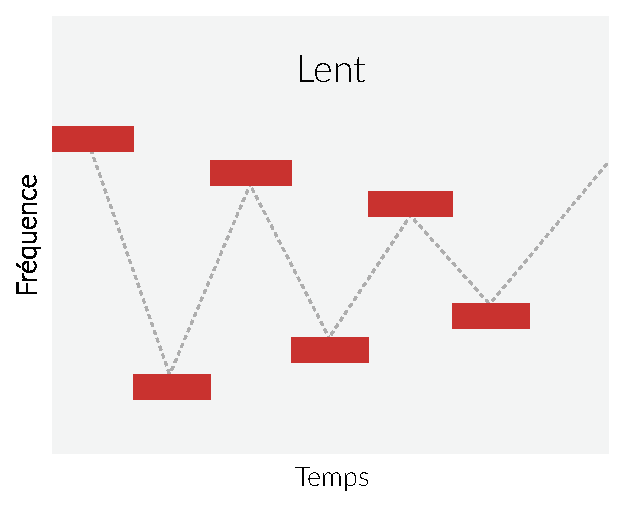
\includegraphics[width=.5\linewidth]{gfx/tonesim_slow}}
        \subfloat[]
        {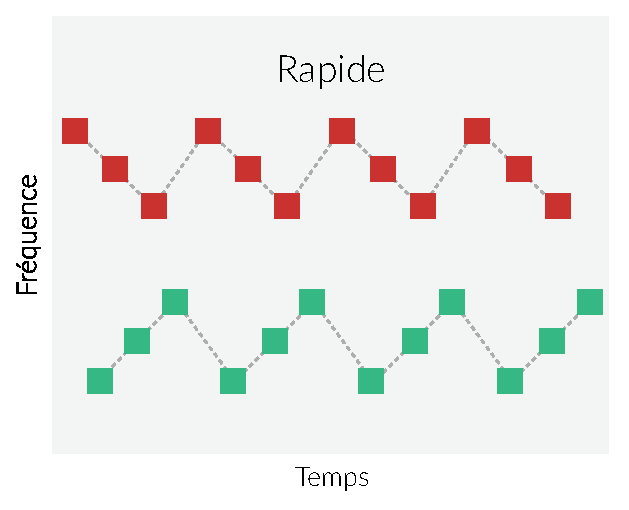
\includegraphics[width=.5\linewidth]{gfx/tonesim_fast}}
        \caption[Groupement séquentiel : proximité temporelle.]{Groupement séquentielle: proximité temporelle. Dans l'exemple (a), la durée entre les événements est telle qu'aucun groupement n'est effectué, les sons sont perçus comme des événements distincts. Dans l'exmple (b) la durée entre les événements est réduite et un groupement s'opère suivant la proximité fréquentielle. Deux flux sont ainsi crées, le premier (rouge) regroupe les sons haute fréquence, et le deuxième (vert) les sons basse fréquence.}\label{fig:tonesim}
\end{figure}

\begin{figure}[bth]
        \myfloatalign
        \subfloat[]
        {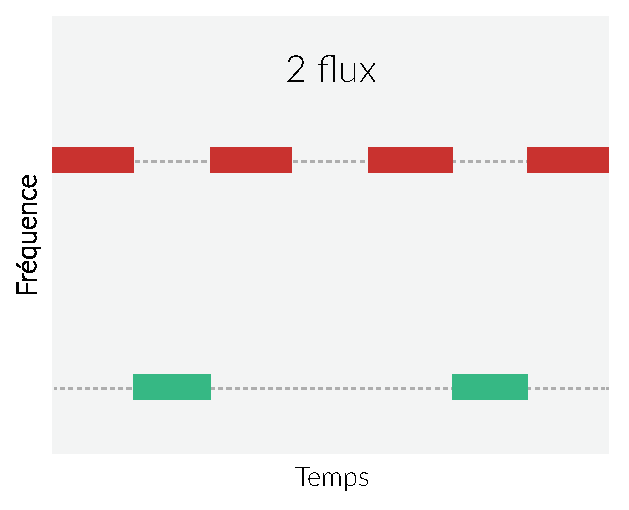
\includegraphics[width=.5\linewidth]{gfx/gallop_2flux}}
        \subfloat[]
        {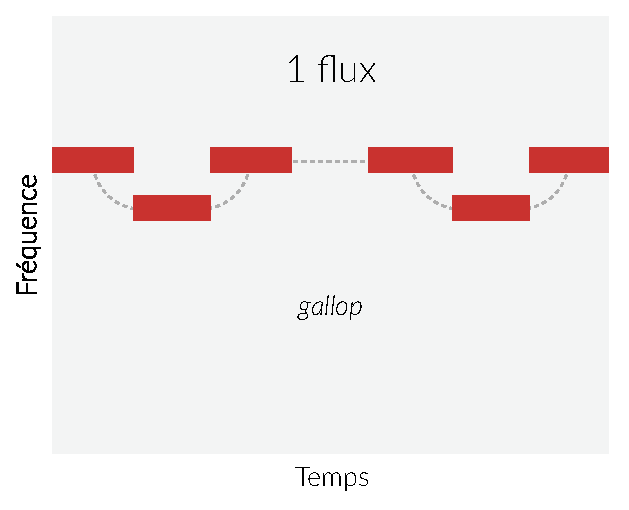
\includegraphics[width=.5\linewidth]{gfx/gallop_1flux}}
        \caption[Groupement séquentiel : proximité fréquentielle.]{Groupement séquentielle: la proximité fréquentielle. Deux groupes de sons sont joués à deux fréquences. Dans l'exemple (a), la distance entre les fréquences des sons est telle que deux flux sont crées, le premier (rouge) regroupe les sons haute fréquence, et le deuxième (vert) les sons basse fréquence. Dans l'exemple (b) la distance entre les fréquences est réduite et un groupement s'opère suivant la proximité fréquentielle. Un seul flux est crée, et l'on perçoit un pattern temporel rappelant le galop d'un cheval.}\label{fig:galop}
\end{figure}

\begin{figure}[bth]
        \myfloatalign
        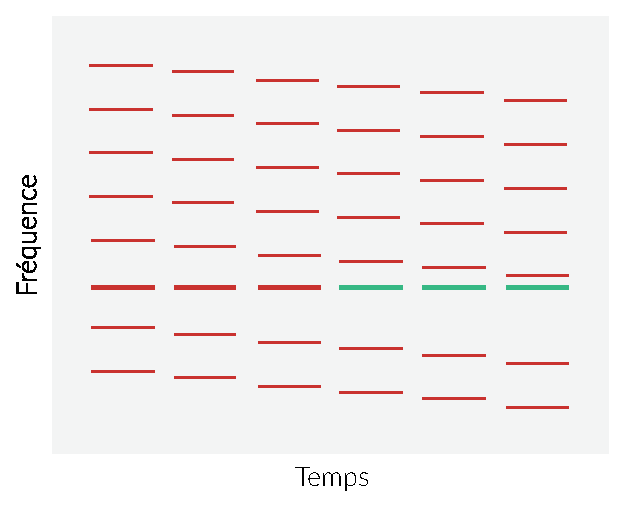
\includegraphics[width=.5\linewidth]{gfx/harmo}
        \caption[Groupement simultané : régularité harmonique]{Groupement simultané : régularité harmonique. Un son complexe est joué plusieurs fois. A chaque occurence, on abaisse les hauteurs de la fréquence fondamentales et des harmoniques de manirèe uniforme. Une harmonique est conservée à fréquence constante (trait gras). Au débur, un flux est crée, \ie~les harminiques et la fréquence fondamentale sont perçus comme étant un seul objet. Au fur et à mesure que la régularité harmonique est brisée, le cerveau tend à percevoir l'harmonique à fréquence constante dans un flux séparé, \ie~comme étant un second objet.}\label{fig:harmo}
\end{figure}

\begin{figure}[bth]
        \myfloatalign
        \subfloat[]
        {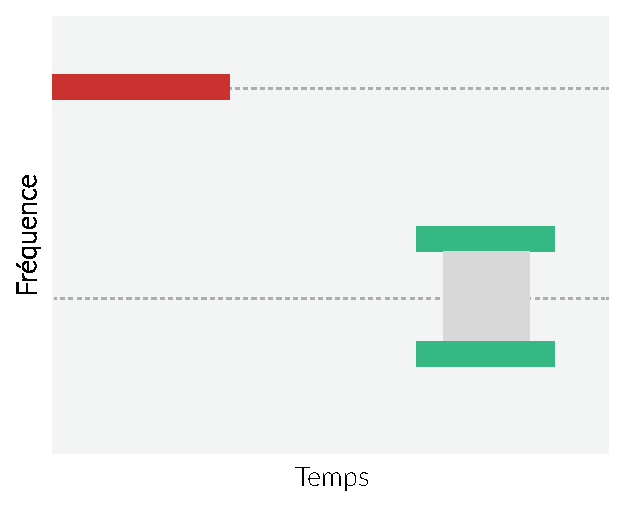
\includegraphics[width=.5\linewidth]{gfx/opn1}}
        \subfloat[]
        {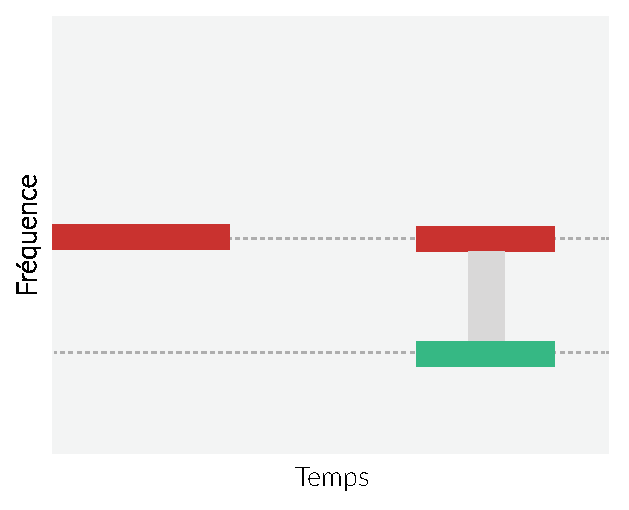
\includegraphics[width=.5\linewidth]{gfx/opn2}}
        \caption[Groupement ancien-plus-nouveau]{Groupement ancien-plus-nouveau. Dans l'exemple (a), les sons A et B ont des fréquences éloignées. Le cerveau génère deux flux, le premier relatif au son A (rouge), et le deuxième comprenant les sons B et C (vert). Dans l'exemple (b), les sons A et B ont la même fréquence. Le cerveau interprète le son B comme étant une continuité du son A. L'attraction entre B et C en est réduite. Le cerveau génère toujours deux flux, le premier regoupant cette fois ci les sons A et B (rouge), et le deuxième le son C (vert).}\label{fig:oldplusnew}
\end{figure}

L'une des notions les plus importante en ASA est le concept de flux auditif (\emph{auditory stream}), que Bregman définit comme ``\,le groupement perceptif que nous faisons des parties du spectre qui vont ensembles\,''.

Contrairement au terme ``\,son\,'', qui peut faire référence tantôt aux réalités physiques des phénomènes acoustiques, aussi bien qu'aux représentations mentales que nous nous en faisons, le flux auditif désigne spécifiquement une entité perceptive.

Le terme flux se veut volontairement généraliste. Ce dernier peut désigner aussi bien un son isolé (un coup de marteau), comme plusieurs sons à condition que ces derniers soient perçus comme formant une seule entité (une série rapprochée de coup de marteau).

On désigne par ``\,formation de flux auditive\,'' (\emph{auditory streaming}) , le processus à l'origine de la création de flux. \citep{winkler2009modeling} propose la définition suivante en ce qui concerne la formation de flux auditif:

\begin{quote}
``\, Un phénomène perceptif dans lequel une séquence de sons est perçue comme étant composée de deux ou plusieurs flux auditifs \,''
\end{quote}

Comme nous venons de le voir, le flux désigne une représentation perceptive d'un son, et à ce titre, il est l'équivalent auditif de l'objet pour la vision \citep[p. 11]{bregman1994auditory}. Cependant, nous notons que la notion de flux, et plus particulièrement la notion de formation de flux, est souvent utilisée dans un contexte ou une dimension temporelle est sollicitée. On parle d'ailleurs de construction de flux  (\emph{build-up of streaming}) pour désigner la période durant laquelle le cerveau accumule des indices afin de générer et stabiliser les flux auditifs  \citep{cusack2004effects,snyder2007toward}. Ainsi dans ce document, nous réservons les termes de flux pour désigner les représentations mentales des stimuli en train d'être traités (intégrés temporellement), de formation de flux auditifs pour désigner les processus perceptives de groupement des sons, mais conservons le terme objet pour désigner de manière générale les représentations mentales stockées en mémoire des phénomènes acoustiques.

Considérant les processus primitifs, on distingue trois stratégies de groupement.

\begin{itemize}
\item \emph{groupement séquentiel}: qui désigne le groupement de sons ne partageant pas un même onset. Dans le cas de sons pures, le groupement séquentiel s'appuie beaucoup sur le principe de \emph{proximité}. Pour des sons pures, il s'agit en particulier de la \emph{proximité} fréquentielle, qui veut que plus deux sons sont proches en fréquence, plus ils auront tendance à être regroupés dans le même flux (\Cf~Figure~\ref{fig:galop}). Pour des sons complexes, c'est plutôt le principe de similarité qui entre en jeux. La \emph{proximité} temporelle, \ie~la durée séparant chaque son, rentre aussi en ligne de compte. Plus cette dernière est faible, plus deux sons auront des chances d'êtres regroupés (\Cf~Figure~\ref{fig:tonesim}).
\item \emph{groupement simultané}: aussi appelé groupement spectral, il désigne le groupement des composantes fréquentielles qui partagent un même onset. Il s'appuie principalement sur la régularité harmonique. Une composante fréquentielle venant briser la suite harmonique tend à être isolée dans un autre flux auditif (\Cf~Figure~\ref{fig:harmo}).
\item \emph{groupement ancien-plus-nouveau}: Cette stratégie est l'application directe du principe de continuité. Lorsque le spectre de l'environnement sonore s’enrichit subitement tout en conservant ses composantes fréquentielles de départ, le cerveau tend à interpréter l'ajout comme une continuation de l'ancien, et à l'intégrer dans le même flux sonore (\Cf~Figure~\ref{fig:oldplusnew}).
\end{itemize}

Dans le cas d'une compétition entre un groupement séquentiel et un groupement simultané, c'est l'organisation issue du groupement séquentiel qui prime (\Cf~Figure~\ref{fig:simvsseq}). Ce phénomène fait sens d'un point de vu écologique. En effet la plupart des sons, et en particulier ceux utilisés pour la communication, n'existent que dans une certaine durée, et sont intermittents. Il est alors nécessaire de faire des associations entre des sons parfois séparés par un intervalle de temps long afin de percevoir le sens du message. \citep{winkler2009modeling}

Les exemples cités plus haut se placent tous dans un contexte \emph{bottom-up}, en évacuant d'éventuels processus attentionnels. Bien que cela ait été encore très peu étudié, il parait cependant évident que ces stratégies de groupement s’opèrent également  dans un contexte \emph{top-down}, en s'appuyant sur une mémoire à plus long terme.

\begin{figure}[bth]
        \myfloatalign
        \subfloat[]
        {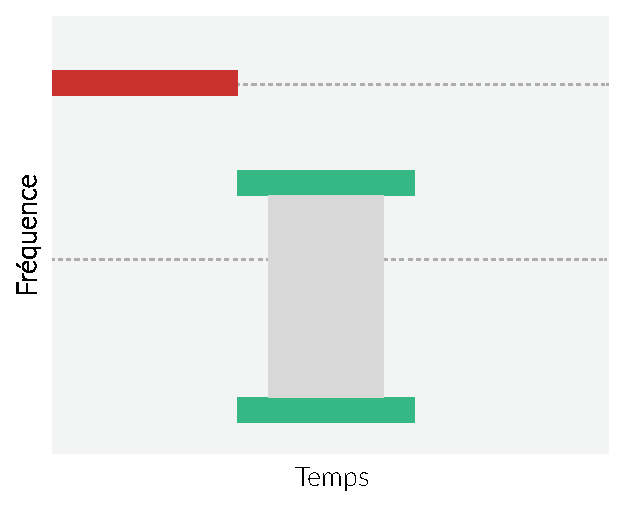
\includegraphics[width=.5\linewidth]{gfx/seqsim1}}
        \subfloat[]
        {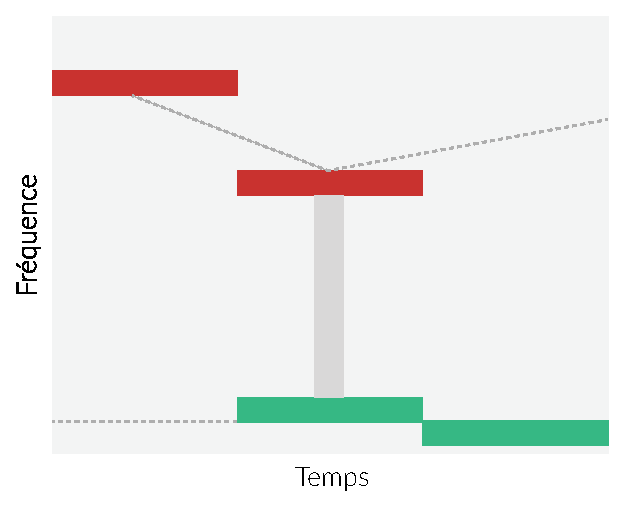
\includegraphics[width=.5\linewidth]{gfx/seqsim2}}
        \caption[Compétition entre groupements séquentiel et simultané]{Compétition entre groupements séquentiel et simultané. Dans l'exemple (a), le cerveau perçoit deux flux, le premier regroupant le son A (rouge) et le deuxième regroupant le sons B et C (vert). Dans l'exemple (b), un quatrième son (D) est ajouté, ce dernier possédant une fréquence très proche de celle de (D). Le groupement sequentiel par proximité fréquentielle entre les couples A-B et C-D est favorisé au détriment du groupement simultané entre les sons B-C.}\label{fig:simvsseq}
\end{figure}

\subsection{Attention et perception}

\subsection{L'approche par les neurosciences}

\section{Le paysage sonore}
\label{sec:paysageSonore}

\subsection{La notion de paysage sonore}

La notion de paysage sonore a été introduite par Schafer dans les années soixante-dix dans son livre \citep{schafer1969new} et détaillée dans l'ouvrage de référence \citep{schafer1977tuning}. La question que se pose Schafer est alors:

\begin{quote}
``\,Quelle est la relation entre l'homme et les sons de l'environnement qui est le sien, et que se produit-il lorsque ces sons viennent à changer ?\,''
\end{quote}

Une première définition du paysage sonore a été donnée par sur celle donnée par 

\begin{quote}
``\,[a]n environment of sound (or sonic environment) with emphasis on the way it is perceived and understood by the individual, or by a society\,'' 
\end{quote}

Aujourd'hui la communauté s'est accordée autour de la définition suivante \citep{aletta2016soundscape}:

\begin{quote}
``\,Un environnement sonore tel qu'il est perçu, expérimenté et/ou compris par un individu ou une communauté, dans son contexte.\,'' \footnote{Cette définition a été publiée dans le cadre de la norme ISO 12913 \citep{iso12913}}
\end{quote}

Ces définitions se veulent volontairement très générale. Tout environnement peut être considéré comme un paysage sonore si tant est qu'on lui associe un ensemble de sons entendu par un sujet donné. Le point capital est d'envisager l’environnement sonore par rapport à l'évaluation subjective de l'auditeur, plutôt que de ne prendre en compte que ses paramètres acoustiques. Schafer explicitait déjà la nécessité de ne plus considérer seulement le bruit, mais également sa perception par les individus qui le subissent ainsi que son contexte dans d'écoute, et ce afin de pouvoir améliorer la qualité de l'environnement. On parle d'environnement sonore lorsque l'on se réfère au phénomène acoustique physique, et de \emph{soundscape} lorsque l'on se réfère à la représentation que l'on se fait de l'environnement.

Ainsi, les études sur les paysages sonores suivent le paradigme de la psychologie cognitive \citep{dubois2006cognitive,maffiolo_caracterisation_1999} (voir~\ref{sec:psychoCog}). L'environnement sonore est décrit en utilisant à la fois des descripteurs acoustiques (mesures), ainsi que des descripteurs perceptifs, l'analyse de l'interaction entre ces descripteurs permettant de comprendre les processus cognitifs mis en œuvre dans l'évaluation perceptive des paysages sonores.

L'approche étant ainsi centrée sur le sujet, les recherches sur les paysages sonores sont par essence interdisciplinaires \citep{davies2013perception,aletta2016soundscape}, faisant appel à des outils et méthodes provenant de champs de recherches variés comme l'acoustique, la psychologie cognitive, la psycho-linguistique, la sociologie, et plus récemment, l’intelligence artificielle.

\subsection{Application à la nuisance sonore urbaine}

La ville a toujours été un environnement bruyant, et ce quelles que soient les époques. Ce qui a par contre évolué, c'est la perception de ce bruit. C'est dans les années 80 que l'association bruit/pollution se fait la plus forte. Le bruit est alors considéré comme une dégradation globale de la qualité de vie. En réponse, les recherches sur les environnements sonores se concentrent sur l'identification des sons responsable du bruit, et sur les moyens permettant d'abaisser leurs niveaux sonores. Plusieurs législations anti-bruit sont ainsi mises en place, la grande majorité ayant pour but de combattre les nuisances sonores en réduisant hauts niveaux d'intensité des sons émis par l'industrie ou les transports.

Mais le problème persiste, et pour cause, le bruit demeure un phénomène subjectif, autrement dit dépendant de l'appréciation l'auditeur. Le bruit est affaire de contexte. Le son d'une sirène peut ainsi agacer comme prévenir d'un danger, et beaucoup de quartiers urbains sont appréciés entre autre grâce à leur atmosphère vivante et festive, qui se traduit souvent par des niveaux sonores élevés. Rappelons d'ailleurs que ville agréable, ne rime pas avec ville silencieuse.  


Corriger l'environnement sonore uniquement suivant des paramètres acoustiques, par définition objectifs (par exemple le niveau sonore), ne suffit donc pas. C'est d'ailleurs maintenant largement accepté que des mesures acoustiques objectives, comme le $L_{Aeq}$ ne peuvent rendre compte seules du confort acoustique \citep{yang2005acoustic,schulte2006soundscape,kang2010semantic,aletta2016soundscape}. Afin d'aller plus loin, il faut envisager le bruit comme un objet cognitif, et non comme un objet physique \citep{guastavino_etude_2003}. Il ne s'agit plus de savoir à partir de quand le bruit n'est plus nuisant, mais pourquoi tel bruit est perçu comme gênant par tel individu. Les recherches sur les environnements sonores urbains se sont ainsi tournées vers la notion de paysage sonore, cette dernière envisageant la nuisance sonore d'une manière plus large, prenant en compte les aspects qualitatifs et sémantiques des phénomènes acoustiques. 

De plus, si beaucoup d’effort sont faits afin de réguler les niveaux bruits des sons non-désirés,  l'approche inverse, \ie~ ajouter des sons positivement connotés reste très peu considérée. Cette approche, consistant à identifier et agir sur les sons acceptés ou plaisants afin d'améliorer la qualité d'un environnement, est nommée l'approche positive par Schafer. De récentes études ont montré des résultats prometteurs, notamment \citep{hong2013designing} qui montre que l'ajout de sons d'oiseaux ou d'eau à des sons de trafics urbain permet de significativement améliorer l'appréciation de ces derniers. \gl{aussi cité \citep{galbrun2012perceptual}}

Depuis 20 ans qu'elle existe, l'approche par les paysages sonores a déjà permis de développer une base de descripteurs qualitatifs et acoustiques grâce auxquels nous jugeons mieux, et sommes mieux à même d'améliorer l'environnement sonore urbain  \citep{kang2006urban,schulte2007soundscape}

Un des enjeux présent de l'analyse des paysages sonores est de relier ces données perceptives, établies à partir d'enquêtes, à des mesures acoustiques, afin de pouvoir établir une politique de réduction du bruit efficace, adaptée à chaque situation \citep{schulte2013soundscape}.
Cependant, le caractère multi-disciplinaire de ces recherches, et l'utilisation de protocole expérimentaux variés pour évaluer l'environnement sonore, rendent l’intégration des résultats difficile \citep{davies2013perception}. De plus, il n'y a toujours pas de consensus sur les descripteurs (acoustiques ou perceptifs) à utiliser pour caractériser un paysage sonore \citep{brocolini2012prediction,aletta2016soundscape}, empêchant la communauté de proposer aux décideurs en matière de politique d'urbanisation, des indicateurs génériques et clairs, ou des modèles, permettant de rendre compte de la qualité d'un paysage sonore.

Récemment plusieurs projets internationaux ont été lancés afin de standardiser les pratiques expérimentales des recherches s’intéressant aux paysages sonores, notamment \emph{ the European Cooperation in Science and Technology Action}\footnote{TD0804, \emph{soundscape of European Cities and Landscapes}: \url{http://www.cost.eu/COST_Actions/tud/TD0804}} \citep{schulte2010soundscape} et \emph{the Positive Soundscape project} \citep{salford2106,davies2013perception}, mais ces problèmes restent à ce jour ouverts \citep{schulte2013soundscape,ribeiro2013heart}.

\subsection{Objectifs et méthodologie}

\subsubsection{L'approche catégorielle}
\label{sec:appCategorielle}

Les objectifs de l'approche catégorielle sont triples. Il s'agit 

\begin{itemize}
\item d'appréhender les principes psychologiques qui sous-tendent la formation des représentations mentales
\item d'objectiver la nature de ces représentations
\item de comprendre l'influence de ces représentations sur le traitement de l'information sonore
\end{itemize}
 
A ce titre, l'approche catégorielle peut être vue comme une approche cognitiviste. 

L'enjeu des approches catégorielle est d'étudier les catégories mentales soit de paysages sonores, soit de sources sonores. Pour ce faire, on a habituellement recourt à deux types d'expérience (\Cf~Figure~\ref{fig:descat}) :

\begin{itemize}
\item \emph{Tâche de description}: On demande au sujet de décrire un environnent sonore \citep{axelsson2005soundscape,raimbault2005urban,guastavino2006ideal,raimbault2006qualitative}, soit de la manière la plus libre possible via une description libre, soit en contraignant la description par le biais d'un questionnaire. Là encore, les réponses aux questionnaires peuvent être libres (questionnaire semi-dirigé) soit à choix forcés (questionnaire dirigé). Plus la description est libre plus on accède à des représentations mentales spécifiques au sujet. A contrario, plus le questionnaire est contraint, plus on accède à des représentations stéréotypées. Ces études s'appuient souvent sur des analyses linguistiques et lexicales pratiquées sur les descriptions des sujets, afin d'en faire émerger catégories. La finesse des descriptions obtenues en laissant de la liberté au sujet dans ses réponses se paye par des données plus difficilement analysables. Ces expériences de descriptions peuvent être réalisées en laboratoire, ou dans un cadre \emph{in situ}.
\item \emph{Tâche de tri ou catégorisation}. Lors d'une tâche de catégorisation, on présente au sujet un ensemble de stimuli sonores, le plus souvent via le biais d'une interface programmée sur ordinateur \citep{maffiolo_caracterisation_1999,guastavino2007categorization}. Ce dernier doit alors organiser ces stimuli en groupes ou paquets, suivant une consigne qui dépend de l'objectif de l’expérience. L'analyse de ces groupes permets de faire émerger des catégories et de comprendre quels sont les attributs perceptifs qui sont à l'origine de l'organisation catégorielle proposée par le sujet. Il est par ailleurs possible de demander au sujet de nommer, voire décrire ces groupes, afin d'acquérir encore plus de connaissance sur la nature des groupements effectués. On parle de catégorisation forcée lorsque que le nombre de groupe, et dans catégorisation libre lorsque le sujet reste libre d'organiser les stimuli comme il l'entend. Ces expériences de tri sont pratiquées en laboratoire, en utilisant habituellement des enregistrements sonores comme stimuli.
\end{itemize}

L'avantage de ces pratiques expérimentales sont doubles:

\begin{enumerate}
\item  elles laissent une grande liberté au sujet dans ces réponses. En particulier, la tâche de catégorisation peut permettre de caractériser des stimuli sans imposer au sujet des dimensions ou attributs particulier à partir desquels évaluer les sons, comme c'est notamment le cas pour l'analyse sémantique différentielle (\Cf Section~\ref{}). En effet, il y a un risque que ces dimensions ne fassent pas sens pour le sujet. 
\item \gl{développer sur \citep{dubois1991semantique} afin de justifier l'utilisation du langage}
\end{enumerate}

\begin{figure}[bth]
        \myfloatalign
        \includegraphics[width=\linewidth]{gfx/desCat}
        \caption{Tâche de description et tâche de tri ou de catégorisation}\label{fig:descat}
\end{figure}

\gl{catégorisation, similarité, mds, analyse discriminante}

\subsubsection{L'approche dimensionnelle}

Au lieu de demander au sujet de décomposer ou trier des environnements sonores en catégories, l'approche dimensionnelle tente elle de caractériser les environnements sur la base de dimensions pré-établies. 

Pour ce faire elle a communément recours à l'analyse sémantique différentielle. Dans ces expériences, le sujet doit noter l'environnement en s'aidant d'échelles bipolaires. Ces échelles, encore appelées de échelle Likert, symbolisent l'ensemble des valeurs pouvant être prises par les différents attributs de la scène sonore entrain d'être évaluée. En ce sens, un ensemble d'échelles peut être vu comme un questionnaire à réponses fermées. En fonction des besoins de l'étude, ces échelles peuvent être discrètes ou continues, paires ou impaires. Cependant dans le cadre de l'évaluation des environnements sonore, on utilise généralement des échelles impaires et graduées suivant 7 \citep{raimbault2006qualitative}, 9 \citep{hall2013exploratory} ou 11 points \citep{ricciardi2015sound}

Le terme sémantique vient du fait que les extrémités des échelles sont décrites par un ou plusieurs mots. Par exemple, \citep{ricciardi2015sound} évalue la qualité de l'environnement et la présence de voitures sur deux échelles de 11 points chacune, possédant respectivement à leurs extrémités les termes désagréable (1) / plaisant (11) (\emph{unpleasant}/\emph{pleasant}) et rare (1) / fréquent (11). Ces termes servent à borner les réponses du sujet afin de s'assurer que tous les sujets interprète de la même manière, \ie~en attribuant  peu ou prou la même valeur à chacune des graduations. Ce fait est néanmoins difficilement vérifiable en pratique, les termes extrêmes pouvant revêtir un sens différent en fonction des sujets.

Ces études peuvent être réalisée en laboratoire via une interface machine, ou bien dans un cadre \emph{in situ} via l'utilisation de questionnaires papiers \citep{jeon2013soundwalk,torija2013application} ou comme c'est de plus en plus le cas, via une application sur téléphone portable \citep{kardous2014evaluation,ricciardi2015sound}. L'immense avantage de cette dernière approche est qu'elle permet d'enregistrer l'environnent que le sujet est entrain d'évaluer, permettant ainsi de circonvenir en partie aux désavantages inhérents aux études \emph{in situ}, notamment en ce qui concerner la reproductibilité des stimuli (\Cf~\ref{sec:ecologique}).

L'avantage non négligeable de l'approche dimensionnelle réside dans le fait que ces résultats soient facilement analysables et interprétables. En effet, évaluer un environnement sonore  en utilisant d'un ensemble d'échelles sémantiques permet d'obtenir une description de ce dernier sous la forme d'un ensemble de descripteurs quantitatifs. Il existe alors quantité de tests statistique, paramétriques ou non-paramétriques (\Cf~\ref{app:analyseStat}), permettant de vérifier l'existence de différences significatives entre tel ou tel type d'environnement sonore \citep{hong2013designing}. De plus cette représentation quantitative permet de tester d'éventuel corrélation entre les descripteurs perceptifs/subjectifs (obtenus par le biais des échelles) et/ou entre des descripteurs acoustique/objectifs (obtenus par le biais de mesures acoustiques, ou via des indicateurs psychoacoustiques issus du traitement du signal). Par exemple, \citep{torija2013application} évalue les corrélations entre 15 descripteurs perceptifs et 49 descripteurs acoustique via l'utilisation du coefficient de Pearson. Cette approche permet également d'envisager l'utilisation de techniques de régression linéaire (\Cf~ref{app:analyseStat}) afin, par exemple, de modéliser la variation d'un descripteur perceptif (l'agrément) en fonction la encore d'autres descripteurs perceptifs (niveau sonore perçu) ou physique ($L_{Aeq}$) \citep{lavandier2006contribution,ricciardi2015sound}.

Enfin, il est également possible de d'analyser directement l'espace décrit par l'ensemble des descripteurs considérés (perceptifs ou physiques). Si l'on cherche à créer des groupes de scènes sonores similaires au sens des descripteurs, il est possible d'avoir recours à des techniques de clustering, comme par exemple le clustering hiérarchique ascendant \citep{torija2013application} ou encore des méthodes non-supervisées inspirées des réseaux de neurones comme les cartes auto-organisée (\emph{self organized map}) \citep{ricciardi2015sound}. Par ailleurs, les différents descripteurs pouvant être très corrélés entre eux, il est également possible d'utiliser des techniques d'analyse de dimensionnalité, comme l'analyse par composante principale, permettant de générer de nouvelles dimensions linéairement non-corrélés, et de sélectionner celles qui expliquent le mieux la variance des données \citep{cain2013development,torija2013application}. Ces nouvelles dimensions n'ayant pas de valeur physique ou perceptive a priori, une inspection qualitative des scènes sonores est alors nécessaire afin de les caractériser.

L'approche dimensionnelle laisse beaucoup moins de  liberté au sujet, ce dernier étant contraint d'utiliser les échelles qui lui sont présentées pour décrire l'environnement, au risque que ces dernières soient mal interprétées, voire ne fassent pas sens. Une description détaillée des échelles, ainsi que l'utilisation de plusieurs mots pour décrire une extrémité permet de diminuer l'impact de ce biais potentiel. \citep{hall2013exploratory} évalue ainsi l'agrément en utilisant une échelle de 9 points dont les extrémités sont décrites par les triplets désagréable-mécontent-insatisfait / agréable-content-satisfait. Ce biais peut encore être réduit en apportant un soin particulier à la sélection des termes extrêmes afin de s'assurer que ces derniers soient bien appropriés, en menant par exemple une expérience intermédiaire sur la base d'un questionnaire libre \citep{guastavino2004perceptual}, potentiellement réalisé en condition \emph{in situ} \citep{kang2010semantic,hong2013designing}, ou en demandant au sujet d'expliquer verbalement sa notation \citep{raimbault2006qualitative}. 

Dans toute épreuve perceptif d'évaluation ayant recourt à l'utilisation d'échelles, il y a un risque que les sujets n'utilisent pas l'échelle de la même manière. Afin de réduire la variance inter-sujet, il est possible de normaliser les données avant de les analyser \citep{defreville2004aactivity,lavandier2006contribution,nielbo2013investigating,hong2013designing}. Cette étape de normalisation est quasi obligatoire lorsqu'il s'agit d'échelles de notation (\eg~attribution d'une note entre 0-10, 0-100 etc $ldots$) ne possédant pas de termes sémantiques aux extrémités. En effet rien ne garantie que la valeur subjective donnée à une note (\eg~5/20) soit la même pour tous les sujets. Dans le cas d'échelle sémantique, le recours à la normalisation est beaucoup moins évident, la présence des termes sémantiques étant déjà là pour réduire les différences d'interprétation. Dans ce cas, l'utilisation de la normalisation peut être la cause d'une perte d'information.

En général, pour un environnement donné, la valeur finale d'une l'échelle est calculée en moyennant les réponses de plusieurs sujets. Pour être valide, cette approche suppose que la distribution des réponses sur l'échelle soit mono-modale. Or il a déjà été montré que ces distributions peuvent être multi-modales, dû entre autre à des différences inter-sujets sur le sens donné aux valeurs de l'échelle, ou simplement à des différences d'appréciation relatives à d'autres facteurs \citep{raimbault2006qualitative}. De plus, l'utilisation de ces échelles suppose que les attributs qu'elles décrivent puissent être évalué de manière linéaire et uni-dimensionnelle, ce qui n'est pas toujours le cas. \citep{raimbault2006qualitative} montre notamment que des échelles sensées évalués la structure temporelle d'une scènes sonore (stable/instable ou figé/évolutif) ne conviennent pas, cette notion n'étant pas compris par les sujets comme étant bipolaire. Ainsi, dans le cadre de l'approche dimensionnel, il est important de s'assurer que:

\begin{enumerate}
\item les échelles soient aptes à décrire les attributs qu'elles décrivent
\item les échelles soient correctement interprétées par les sujets
\end{enumerate}

\subsection{Catégorisation de sources et environnements sonores}

\subsubsection{Catégories de sources sonores}

G0: \citep{gaver1993world} interaction
G1: \citep{guastavino2006ideal,szeremeta2009analysis} decomposition du soundscape, analyse lexical (preciser pour guastavino que la notion d'idéal est liée ici à l'agrément)
G2: \citep{Houix03f,guastavino2007categorization,gygi2007similarity,houix_lexical_2012} catégorisation de source sonores

\subsubsection{Catégories de paysages sonores}

G1: \citep{maffiolo_caracterisation_1999} événement et amorphe
G2: \citep{jeon2013soundwalk}
G3: \citep{brown2011towards}

\subsection{Classification de sources et environnements sonores}

\subsubsection{Classes de sources sonores}

G1: \citep{niessen2010categories,park14} sur la base de catégories
G2: \citep{yang2013psychoacoustical} psychoacoustique

\subsubsection{Classes de paysages sonores}

G1: \citep{rychtarikova2013soundscape,torija2013application} clustering sur la base d'indicateurs acoustiques.

\subsection{Analyse et Modélisation des propriétés perceptives des paysages sonores}
\gl{A refaire, il s'agit bien de descripteurs perceptifs, a bouger dans analyse dimensionnelle}
Le paysage sonore est un objet perceptif. Ces propriétés perceptives étant multiples, l'analyse de l'évaluation des paysages sonores demande de se concentrer sur l'une de ces propriétés. Analyser une de ces propriétés (\eg~l'agrément) c'est trouver les descripteurs perceptifs (\eg~niveau sonore perçue) et physique (\eg~niveau sonore mesuré) dont la modification affecte la valeur de la propriété perçue. Une étape plus ambitieuse dans l'étude des propriétés et de proposer des modèles prédictifs, permettant de prédire l’évolution des propriétés, sur la base là encore de descripteurs acoustiques et physiques.

Dans tous les cas, ces études demandent à des sujets d'évaluer sur des échelles sémantiques la propriété étudié, ainsi que les éventuels descripteurs perceptifs testés.

Nous détaillons dans la suite de cette section quatre propriétés particulièrement étudiées. Il est a noter qu'il n'existe pas de consensus dans la communauté sur 1) la définition de ces propriétés et 2) les pratiques expérimentales permettant de les étudier. Par ailleurs, certaines de ces propriétés ont un caractère plus général que d'autres, certaines pouvant même servir de descripteurs perceptifs pour d'autres propriétés

\subsubsection{Gêne et bruit}

La gêne provoquée par un paysage sonore, et en particulier par un paysage sonore urbain a peut être été la propriété perceptive la plus étudiée. Ce fait est notamment lié au besoin pressant de trouver une solution à la pollution sonore en ville. Une récente étude indique d'ailleurs que 86\% des français sont gêner par le bruit ambiant lorsqu'ils se trouvent chez eux \citep{noiseFrench}.

États de l'art \citep{marquis2005noisea,marquis2005noiseb}

Premier groupe d'étude sur le trafic et le bruit \citep{gille2016testing,gille2016noise,gille2016dose,morel2016noise,trolle2015perception,marquis2015simulated,klein2015spectral,}

\subsubsection{Qualité sonore}

G1 \citep{brocolini2012prediction,ricciardi2015sound}
G2 \citep{hong2013designing} utilise la notion de préférence, lien avec le confort acoustique.
G3 \citep{ozcevik2012laboratory}
G4 \citep{yu2010factors} preference
G5 \citep{nilsson2006soundscape,nilsson2007acoustic}

\subsubsection{Agrément}

G1: \citep{garcia2012validation} 
G2: \citep{lavandier2006contribution}
G3: \citep{guillen2007importance}

\subsubsection{Confort acoustique}

G1: \citep{yang2005acoustic,meng2013field}
G2: \citep{jeon2011non,jeon2013soundwalk}
G3: \citep{tse2012perception}
G4: \citep{yu2009modeling} modèle du confort

\subsubsection{Calme et tranquillité}

G1: \citep{delaitre2012definition} définition du concept
G2: \citep{pheasant2008acoustic,pheasant2009validation}
G3: \citep{memoli2008soundscape}
G4: \citep{de2006quiet,de2013characterizing} influence musicale
G5: \citep{payne2013production} notion de restauration

\subsubsection{Propriétés combinées}

G1: \citep{davies2013perception}
G2: \citep{cain2013development}
G3: \citep{axelsson2010principal}
G4: \citep{hall2013exploratory} émet des réserves sur la justesse de cette approche.

\subsubsection{Autre descripteurs}

G5: \citep{kang2010semantic} autres

\subsubsection{Prendre en compte les contributions séparées des différentes sources sonores}

G0: \citep{defreville2004aactivity} première étude
G1: \citep{marquis2015simulated} bruit
G2:  \citep{lavandier2006contribution,guillen2007importance} agrément
G3:  \citep{nilsson2007soundscape,ricciardi2015sound} qualité

\subsubsection{Influence d'attributs extra-sonores}

G1: Contexte environnementale (température, chaleur, humidité), \citep{meng2013field,jeon2011non}
G2: Contexte socio-culturel \citep{hall2013exploratory,yu2010factors}
G2: Contexte socio-culturel \citep{guillen2007importance} pas d'effet
G3: Contexte spatial \citep{hall2013exploratory}
G4: affordances/appropriateness \citep{hall2013exploratory}

\subsubsection{Réponse physiologique}

G1: \citep{hume2013physiological}

\section{Événements et textures sonores}

\subsection{Définition}

S'éloignant de l'approche des paysages sonores, plusieurs étude se sont concentrées sur l'analyse perceptive d'une certaine catégorie de sons appelée texture sonore.

Pour définir la texture sonore, nous nous appuyons sur la définition donnée par \citep[p. 25]{saint1995classification}:  

\begin{itemize}
\item ``\, Les textures sonores sont des objet composites, formées d'éléments de base appelés atomes\,''
\item ``\, Les atomes apparaissent suivant un pattern haut-niveau pouvant être soit périodique (galop), soit aléatoire (pluie), voire les deux\,''
\item ``\, Les caractéristiques haut niveaux des textures restent constantes sur de de longue périodes de temps, ce qui implique qu'elles ne peuvent comporter aucun message complexe\,''
\item ``\, Le pattern haut-niveau doit être présenté au moins une fois dans sa totalité pendant une période de temps n’excédant pas les quelques  secondes. Cette période est nommé période d'attention (\emph{attention span})\,''
\end{itemize}

Cette définition est avant tout morphologique, la texture étant définie en fonction de ses caractéristiques physiques. Cette approche vient du fait que la texture a d'abord été étudiée dans le cadre du traitement du signal, beaucoup d'application multimédia ayant besoin de  modèles permettant de synthétiser de telle sons \citep{schwarz2011state}. La notion de texture s'oppose intuitivement à celles d'événement sonore ou de séquence d'événements. Par opposition, l'événement est vu comme un élément discret, un son court et non homogène.

C'est la notion d'information transmise qui semble être capitale pour faire la distinction entre les textures et les séquence d'événements. Les caractéristiques des textures restant stables au cours du temps, l'information transmise finit éventuellement par atteindre une asymptote. A contrario, une succession d'événements distincts, comme c'est le cas pour une séquence musicale ou de parole, transmets de plus en plus d'information (\Cf~Figure~\ref{fig:texture}). En poussant le raisonnement à L’extrême, le bruit blanc peut être vu comme la représentation la plus ``\,pure\,'' d'une texture, ce dernier ne portant ainsi quasi plus d'information.

\begin{figure}[bth]
        \myfloatalign
        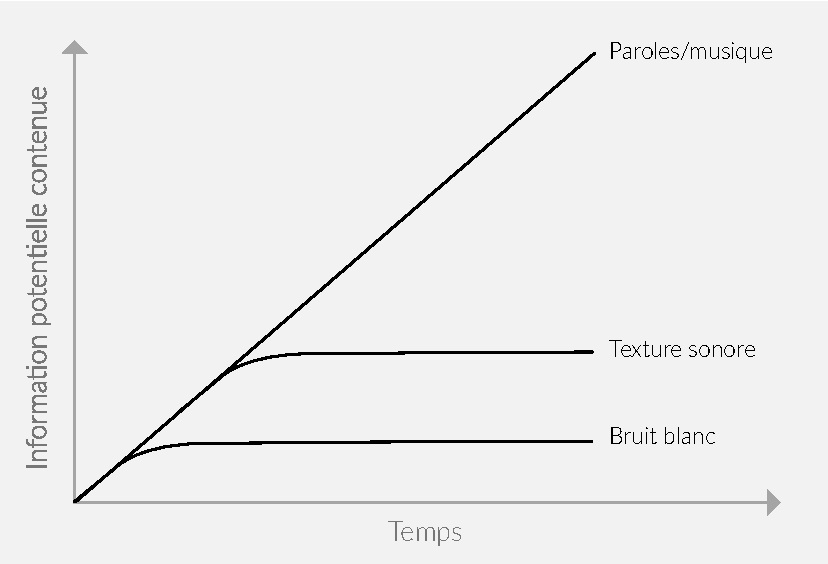
\includegraphics[width=\linewidth]{gfx/texture}
        \caption[Information potentielle contenue dans les séquences d'événements, les textures, et le bruit]{Information potentielle contenue dans les séquences d'événements, les textures, et le bruit. D'après \citep{saint1995classification}}\label{fig:texture}
\end{figure}

\subsection{Percevoir les textures}

Contrairement aux événements sonores, la texture est un objet simple, dont le traitement cognitif ne requière pas une analyse poussée. Ce point a été notamment prouvé par les travaux de Josh H. McDermott et ses co-auteurs \citep{mcdermott2011sound,mcdermott2013summary}. A l'aide d'un modèle de texture, inspiré du fonctionnement des premières étapes du système auditif humain allant de la cochlée jusqu'au thalamus, ils ont pu re-synthétiser des textures sonores en ne servant que de statistiques simples calculés à partir de représentations temps-fréquence de signaux de textures enregistrés. Dans un premier temps, la capacité des sujets à identifier les textures synthétisées a été testée \citep{mcdermott2011sound}. Les résultats ont montré que les sons de synthèse étaient aussi bien identifiés au les sons enregistrés, démontrant ainsi que les statistiques du signal sont utiles d'un point de vu cognitif à la reconnaissance. Dans le cas des textures, elles constitueraient même l'information primordiale, le cerveau faisant fi de toute autre représentations plus détaillées \citep{nelken2013ear}.

Dans une seconde expérience, \citep{mcdermott2013summary} les sujets ont dû reconnaître, parmi une triade de sons synthétisés, celui produit par une source différente (\ie un type de texture différent, \Cf~Figure~\ref{fig:textureMcder}). Les résultats montrent que la capacité de discrimination est fonction de la durée des textures. Plus cette dernière est élevée, plus la capacité à discriminer est importante.  Ce résultat valide les hypothèses formulées par \citep{saint1995classification} sur l'existence d'une période d'attention, nécessaire au cerveau pour comprendre le stimuli comme une texture, et ainsi l'analyser sur la base de statistiques extraites. Il y aurait donc bien dans le processus de traitement, une prise de décision quant à savoir si le stimuli est une texture ou un événement.

Le fait que le jugement perceptif s'améliore avec la durée des stimuli est un principe bien connue en perception des sons\citep{moore1973frequency}. Dans une troisième expérience, \citep{mcdermott2013summary} montre que ce fait n'est pas tout le temps vrai dans le cas des textures. Cette fois ci il demande au sujet de se prononcer sur trois exemplaires provenant d'un même type de texture (\eg~trois sons synthétisés de pluie). Parmi ces trois exemplaires, deux ont été produits à partir des mêmes statistiques extraites, il s'agit pour le sujet d'identifier celui qui a été généré a partir d'un jeu de statistique différent (Figure~\ref{fig:textureMcder}). Les résultats montrent dans ce cas que la capacité des sujets à discriminer le bon stimulus décroît avec la durée des stimuli. Ce fait qui peut sembler contre intuitif, est une nouvelle preuve que le cerveau traite les textures sur la base d'une information réduite. Plus les stimuli sont long, plus le cerveau les interprète comme étant des textures, et les traite sur la base de statistiques simples,  l'extraction de ces dernières ayant pour effet de gommer les différences fines existant entre les stimuli. Si on part du principe que le signal sonore est analysé suivant des fenêtres d'intégrations successives \citep{yabe1998temporal,poeppel2003analysis}, alors plus les stimuli sont long, plus le cerveau tend à garder en mémoire une information dégradée, ne permettant plus de faire la distinction entre des stimuli similaires.

\begin{figure}[bth]
        \myfloatalign
        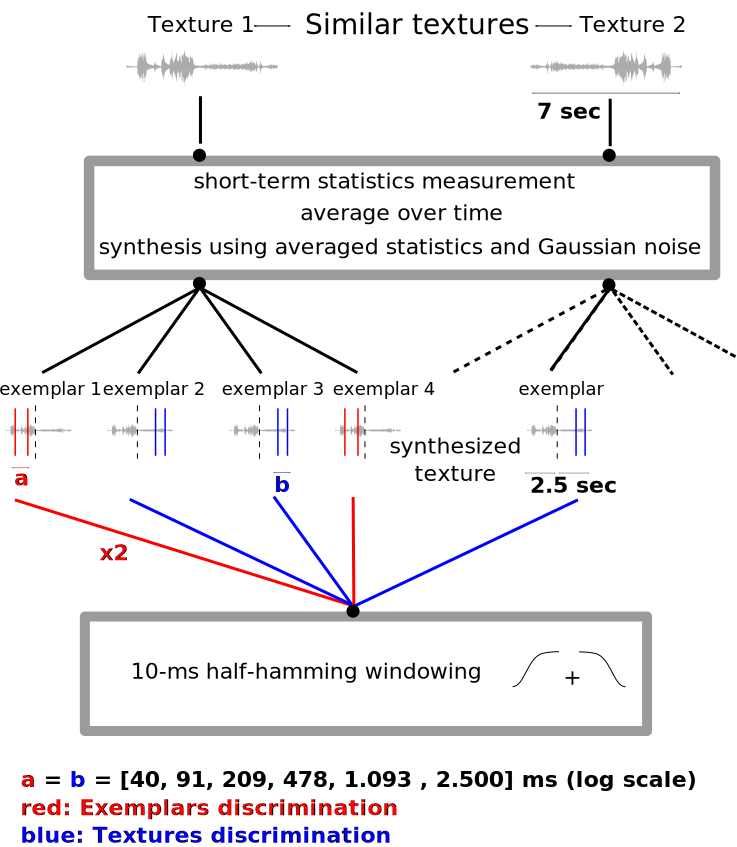
\includegraphics[width=\linewidth]{gfx/mcder}
        \caption[Plannification expérientale de l'expérience de discrimination de textures sonore et d'exemplaires de textures sonores]{Plannification expérientale de l'expérience de discrimination de textures sonore et d'exemplaires de textures sonores, menée par \citep{mcdermott2013summary}}\label{fig:textureMcder}
\end{figure}

Une des avancés majeures de ces études est qu'elles apportent de nouvelles réponses sur la nature des représentations sonores stockées en mémoire. Dans le cas des textures, il s'agirait ainsi de descripteurs bas-niveaux, exprimés sous la forme de statistiques simples. Cette découverte fait sens d'un point de vue écologique, car elle respecte le principe d'économie de moyen. Le cerveau, reconnaissant que les caractéristiques des textures n'évoluent pas au cours du temps, ne conserve en mémoire qu'une information condensée, qui lui permet pourtant de traiter des sons potentiellement longs. 

Il a été montré que le cerveau peut stocker bien plus que des statistiques.  \citep{agus2010rapid} a montré qu'un bruit blanc, écouté de manière répété, pouvait être reconnu encore plusieurs semaines après l'écoute, et ce parmi d'autres bruits blancs. Dans ce cas le cerveau emmagasine bien la totalité du signal acoustique.

\subsection{Période d'attention}

Dans nos travaux nous nous sommes également penchés sur cette notion de période d'attention. En poussant cette vision composite à l’extrême, une texture peut être vu comme un empilement d’événements sonores qui cessent d'être perçus de manière distincte, dès lors que ces derniers forment un tout homogène et stable. 

Nous avons suivi cette idée afin de bâtir un protocole permettant de d'analyser la période d'attention. Nous faisons l'hypothèse qu'à partir du moment ou un événement peut être isoler d'un mixture d'événements du même type, le cerveau ne perçoit plus la mixture comme une texture, mais comme une succession d'événement.

Nous avons monté une expérience de reconnaissance de type oui/non (\Cf~\ref{app:xp_texture} pour une description exhaustive de l'expérience). Chaque stimuli est composé d'un son cible, suivi d'une séquence d'événement enchevêtrés de 6 secondes (\Cf~\ref{fig:xptexture}.a). L'objectif pour le sujet est d'indiquer si oui ou non il a entendu le son cible dans la séquence d’événements.

Les séquences sont des sons de trafic, simulés en agglomérant des sons isolés de voiture. La simulation est contrôlée par un paramètre réglant l'espacement temporel inter-onset moyen entre les événements. Cinq valeurs d'espacement sont considérées: $0.1$, $0.3$, $0.5$, $0.7$ et $0.9$ secondes. Les sons isolés de voiture ont tous une durée de $1$ seconde. Pour chaque espacement, nous simulons 20 séquences de trafics, chaque sujet devant alors écouter 100 stimuli. La moitié de ces stimuli sont des pièges, le son cible y étant absent. Nous mesurons les performances des sujets en utilisant la mesure de sensitivité $d'$ (\Cf~Figure~\ref{fig:xptexture}.b). Les résultats montrent que la mixture cesse d'être perçue comme une texture à partir d'un espacement de 0.42 secondes, soit la durée moyenne des événements utilisés (\Cf~Figure~\ref{fig:xptexture3}).

\begin{figure}[bth]
        \myfloatalign
        \subfloat[]
        {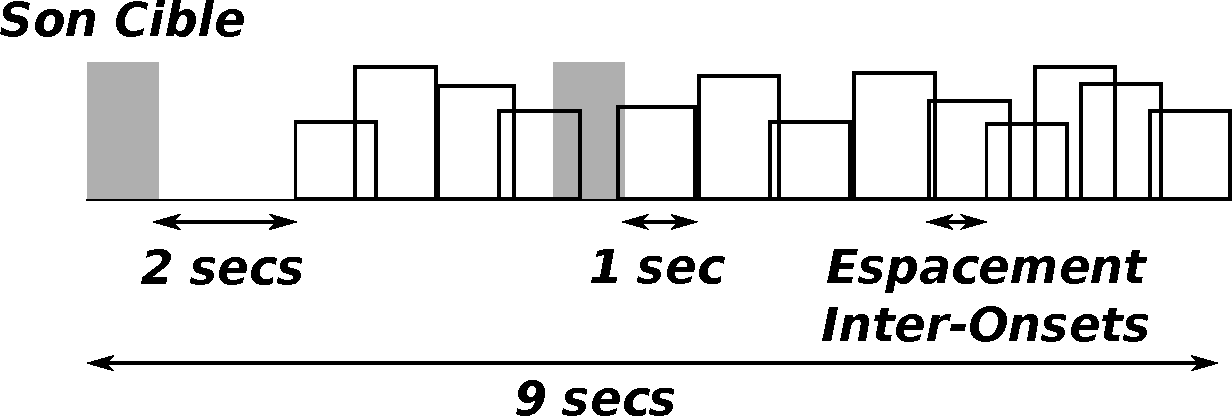
\includegraphics[width=.5\linewidth]{gfx/xpTexture1}}
        \subfloat[]
        {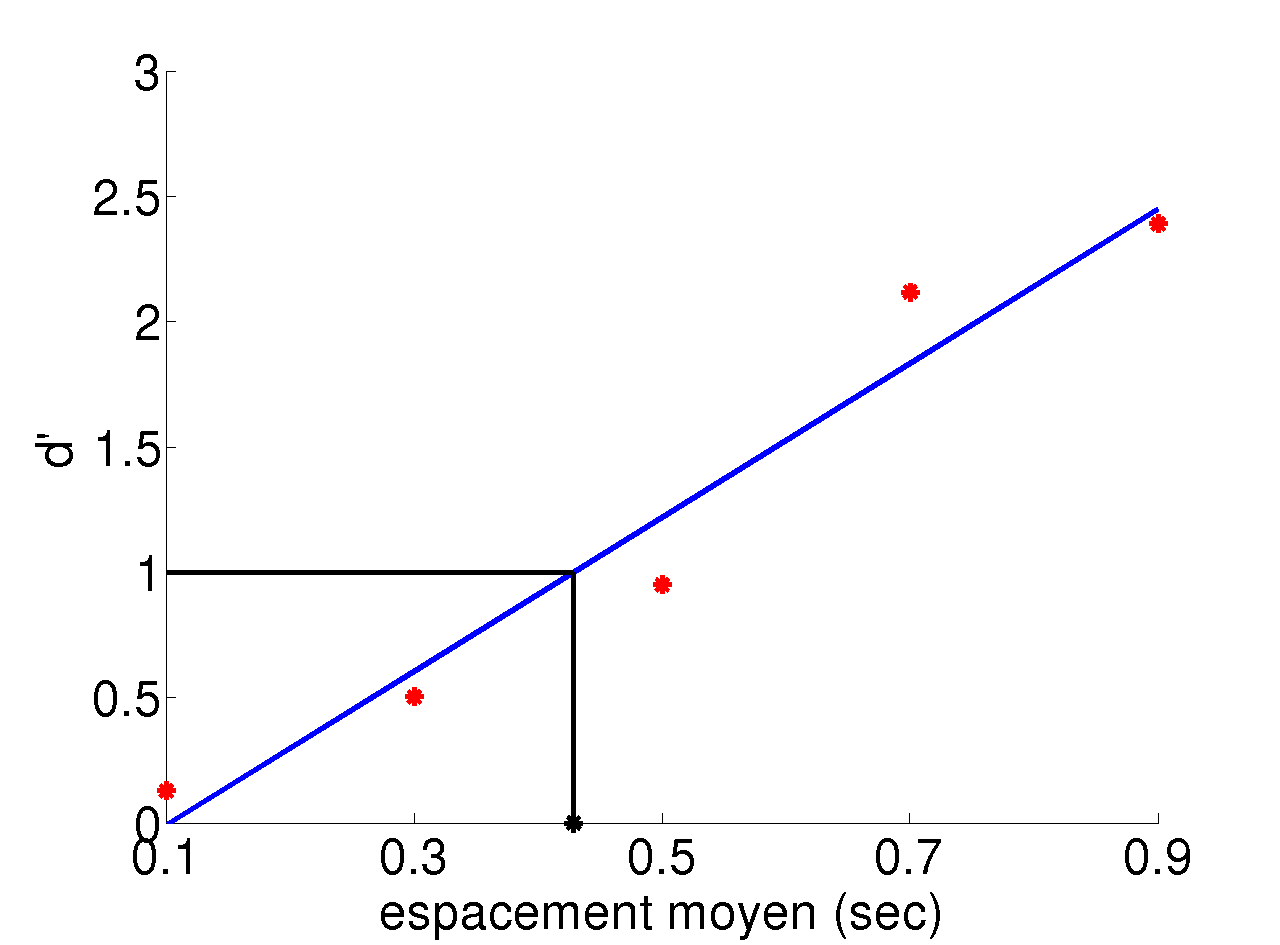
\includegraphics[width=.5\linewidth]{gfx/xpTexture3}}
        \caption[Experience sur la période d'attention]{Experience sur la période d'attention. (a) la nature des stimuli utilisés. (b) le seuil d'espacement moyen permettant de faire la distinction entre une séquence d'événements et une texture}\label{fig:xptexture}
\end{figure}


\subsection{Connexion}


Il est possible de faire des connexions entre les notions de textures/événements, et celles des scènes amorphes/événementielle mises en lumière par \citep{maffiolo_caracterisation_1999}. Pour la notion de texture, nous sommes très proches de celle des séquences amorphes
De même, les séquences événementielles peuvent être vue comme des séquences composées soit uniquement d'événements, soit d'événements et de textures, la présence d'événements, porteurs d'une information plus riche, primant sur la nature des processus mis en œuvre. 

Cette dimension événement/texture est cependant orthogonale à celle de ``\,bruit de fond\,'' / ``\,événements de premier plan\,'' (\emph{background}/\emph{foreground}), utilisée dans le langage courant pour discriminer l’environnement urbain. Concernant les notions de background et de foreground, nous considérons que l'une et l'autre peuvent être vue comme des flux auditifs. Un flux auditif peut être composée de textures et d’événements regroupés dans le but de faciliter le traitement auditif de la scène. 

%*****************************************
%*****************************************
%*****************************************
%*****************************************
%*****************************************

%************************************************
\chapter[Un modèle morphologique]{Un modèle morphologique de scènes sonores environnementales}\label{ch:psycho_model} 
%************************************************

\section{Motivations}

\subsection{Analyse sensorielle}
\label{sec:ch4_anaSo}

Comme nous l'avons vu à la section~\ref{sec:ch3_appCatDim}, l'étude expérimentale des paysages sonores adopte deux approches:

\begin{itemize}
\item l'approche catégorielle: la mise en évidence des catégories d'environnements ou sources sonores;
\item l'approche dimensionnelle: l'identification des dimensions perceptives engagées dans les processus cognitifs, et des indicateurs dont elles dépendent.
\end{itemize}

Ces approches s'inscrivent dans des démarches différentes:

\begin{itemize}
\item l'approche catégorielle veut identifier les objets d'intérêt  de l'environnement sonore;
\item l'approche dimensionnelle veut identifier les éléments caractérisant les qualités affectives perçues d'une scène.
\end{itemize}

Si l'on interroge les influences qu'ont les différents éléments constituant une scène sur les qualités affectives perçues, alors les deux approches se rejoignent naturellement. L'approche catégorielle permet d'établir la liste des éléments d'intérêt, laquelle liste peut servir de base à une annotation des stimuli utilisés par l'approche dimensionnelle afin d'étudier les contributions spécifiques de leurs éléments respectifs.

Nous pensons que la simulation offre un cadre expérimental élégant permettant de faire le lien entre les deux approches \gl{TODO: plus insister ?}.

D'une part, comme illustré à la figure~\ref{fig:paradigmeSimu1}, la simulation peut être vue comme l'approche inverse des épreuves catégorielles (\cf~Section~\ref{sec:ch3_appCategorielle}). Quand les épreuves catégorielles discrétisent l'environnement sonore sur la base d'un tri et/ou d'une description verbale réalisés  par un sujet, la simulation, elle, recompose cet environnement, à partir d'une banque imposée de sons isolés. Ainsi, les catégories sonores, point de sortie des épreuves catégorielles, constituent-elles la banque de sons, point d'entrée de la simulation.

D'autre part, la finalité de la simulation est de produire un environnement complet, dont la partition (\cf~Section~\ref{sec:ch4_modelDes}), \ie~ses caractéristiques structurelles et compositionnelles, est parfaitement connue. Les stimuli ainsi produits peuvent être utilisés par l'approche dimensionnelle, afin d'étudier de manière fine les contributions des différents éléments.

La simulation se pose donc comme un outil intermédiaire, faisant le lien entre les connaissances issues des études adoptant l'approche catégorielle, et les stimuli requis par l'approche dimensionnelle.

La simulation présente d'autres intérêts:

\begin{itemize}
\item \emph{intérêt pratique}: afin d'étudier l'importance relative des différentes sources, il est indispensable de disposer de stimuli dont la partition est connue. Une première solution, adoptée par \citep{lavandier2006contribution}, a été d'annoter les stimuli. L'annotation cependant est une solution limitée: 
\begin{enumerate}
\item l'opération est fastidieuse, longue, et difficile à mettre en œuvre sur de grandes banques de données;
\item connaître la position des différentes sources dans une mixture sonore ne permet pas d'isoler leurs caractéristiques physiques respectives, et donc de calculer des indicateurs acoustiques dédiés. En traitement du signal, la séparation des sources reste un problème ouvert\gl{TODO: citation}.
\end{enumerate}

Par la simulation, nous obtenons directement le stimuli et son annotation. Qui plus est, celle-ci est produite par le sujet lui-même, et non par un tiers. \gl{Par ailleurs, le fait de posséder les sons isolés permet de facilement calculer des indicateurs acoustiques spécifiques à chaque source sonore.}

\item \emph{intérêt écologique}: la validité écologique des stimuli est un problème fondamental en analyse sensorielle. Dans le cas de l'analyse des qualités affectives perçues, où l'on demande au sujet ``\,que pensez vous de la qualité $Q$ de cet environnement\,'', il s'agit de garantir que les stimuli proposés fassent sens par rapport à la représentation mentale que le sujet se fait: 

\begin{itemize}
\item  du monde sonore; 
\item  de la qualité $Q$. 
\end{itemize}

Il est possible, dans les approches classiques, de résoudre ces problèmes en étudiant de manière préalable les stimuli à enregistrer (\cf~Section~\ref{sec:ch3_ecologique}). 

La simulation, en renversant la question posée (``\,générer un environnement qui correspond à une certaine valeur de $Q$\,''), garantit la validité écologique des stimuli, par définition connectés à la représentation sonore du sujet, \gl{à condition que la banque de données et l'outil de simulation soient suffisamment expressifs}.

\item \emph{représentativité des stimuli}: toute étude sensorielle, qu'elle soit \emph{in situ} ou en laboratoire, doit sélectionner un nombre restreint d'environnements sonores à évaluer. Il s'agit, tant que faire se peut, de garantir que le substrat de stimuli proposé soit représentatif de l'ensemble des environnements étudiés, un déséquilibre dans l'élaboration dudit substrat pouvant affecter, \emph{in fine}, l'évaluation des stimuli. 

Dans le cas des études sur la perception des environnements urbains, il est d'usage d'isoler des zones d’intérêts (parc, rue, place, \cf~Section~\ref{sec:ch3_ecologique}), et de répartir équitablement les stimuli parmi ces zones. \gl{Cependant, l'environnement d'une même zone est changeant, aussi bien si l'on considère le type de source présent, que si l'on considère la structure des patterns temporels émis par ces sources (\eg~pour une même rue passante, un son de trafic sera plus dense, composé de plus d'événements de voiture à la fin des horaires de travail). Il est donc nécessaire de contrôler la diversité des sources qui y occurrent ainsi que la diversité structurelle de leurs séquences d'émission}, d'autant plus si l'on cherche à étudier l'influence spécifique des différentes sources. Cette étape est complexe.

Si la structure interne des paysages sonores est variable, la diversité des sources sonores qui les composent est plus contrôlable. Des environnements sonores de parcs et de rues peuvent comprendre des voix humaines, des bruits de pas, des sons de voitures etc. Seules les caractéristiques physiques, ainsi que les patterns d'occurrences de ces sources, vont varier. Évaluer des scènes simulées, à partir d'une banque de sons isolés (sources sonores), peut constituer une solution au problème de la diversité des stimuli. Considérons l'étude de l'agrément sonore dans l'environnement urbain. Dans un premier temps, les stimuli sont obtenus via une épreuve de simulation. Dans cette simulation, seule la qualité affective des stimuli est fixée (agréable/désagréable). Les sujets construisent alors les scènes directement en fonction de l'image qu'ils se font d'un environnement urbain agréable/désagréable, adaptant ainsi la structure de la scène à la qualité de l'environnement. Dans un deuxième temps, les scènes ainsi élaborées peuvent constituer des stimuli pour une analyse sémantique différentielle de l'agrément. Cette approche est celle utilisée dans nos travaux (\cf~Chapitre~\ref{ch:psycho_xp}). 

Enfin, la plupart des environnements que nous percevons sont relativement neutres, et ne provoquent pas en nous de réactions particulières. Il peut n'être pas évident d'évaluer des dimensions perceptives comme l'agrément, la gêne ou le confort, de ces environnements. Des scènes simulées, sur la base d'une qualité affective imposée (\eg~agréable), proposent, quant à elles, des versions stéréotypées des environnements ainsi qualifiés. On peut voir dans ces scènes un ``\,résumé cognitif\,'', riche et condensé des environnements étudiés. Isoler les éléments d'intérêt de ces scènes peut s'avérer plus facile.

\end{itemize}

\begin{figure}[t]
        \myfloatalign
        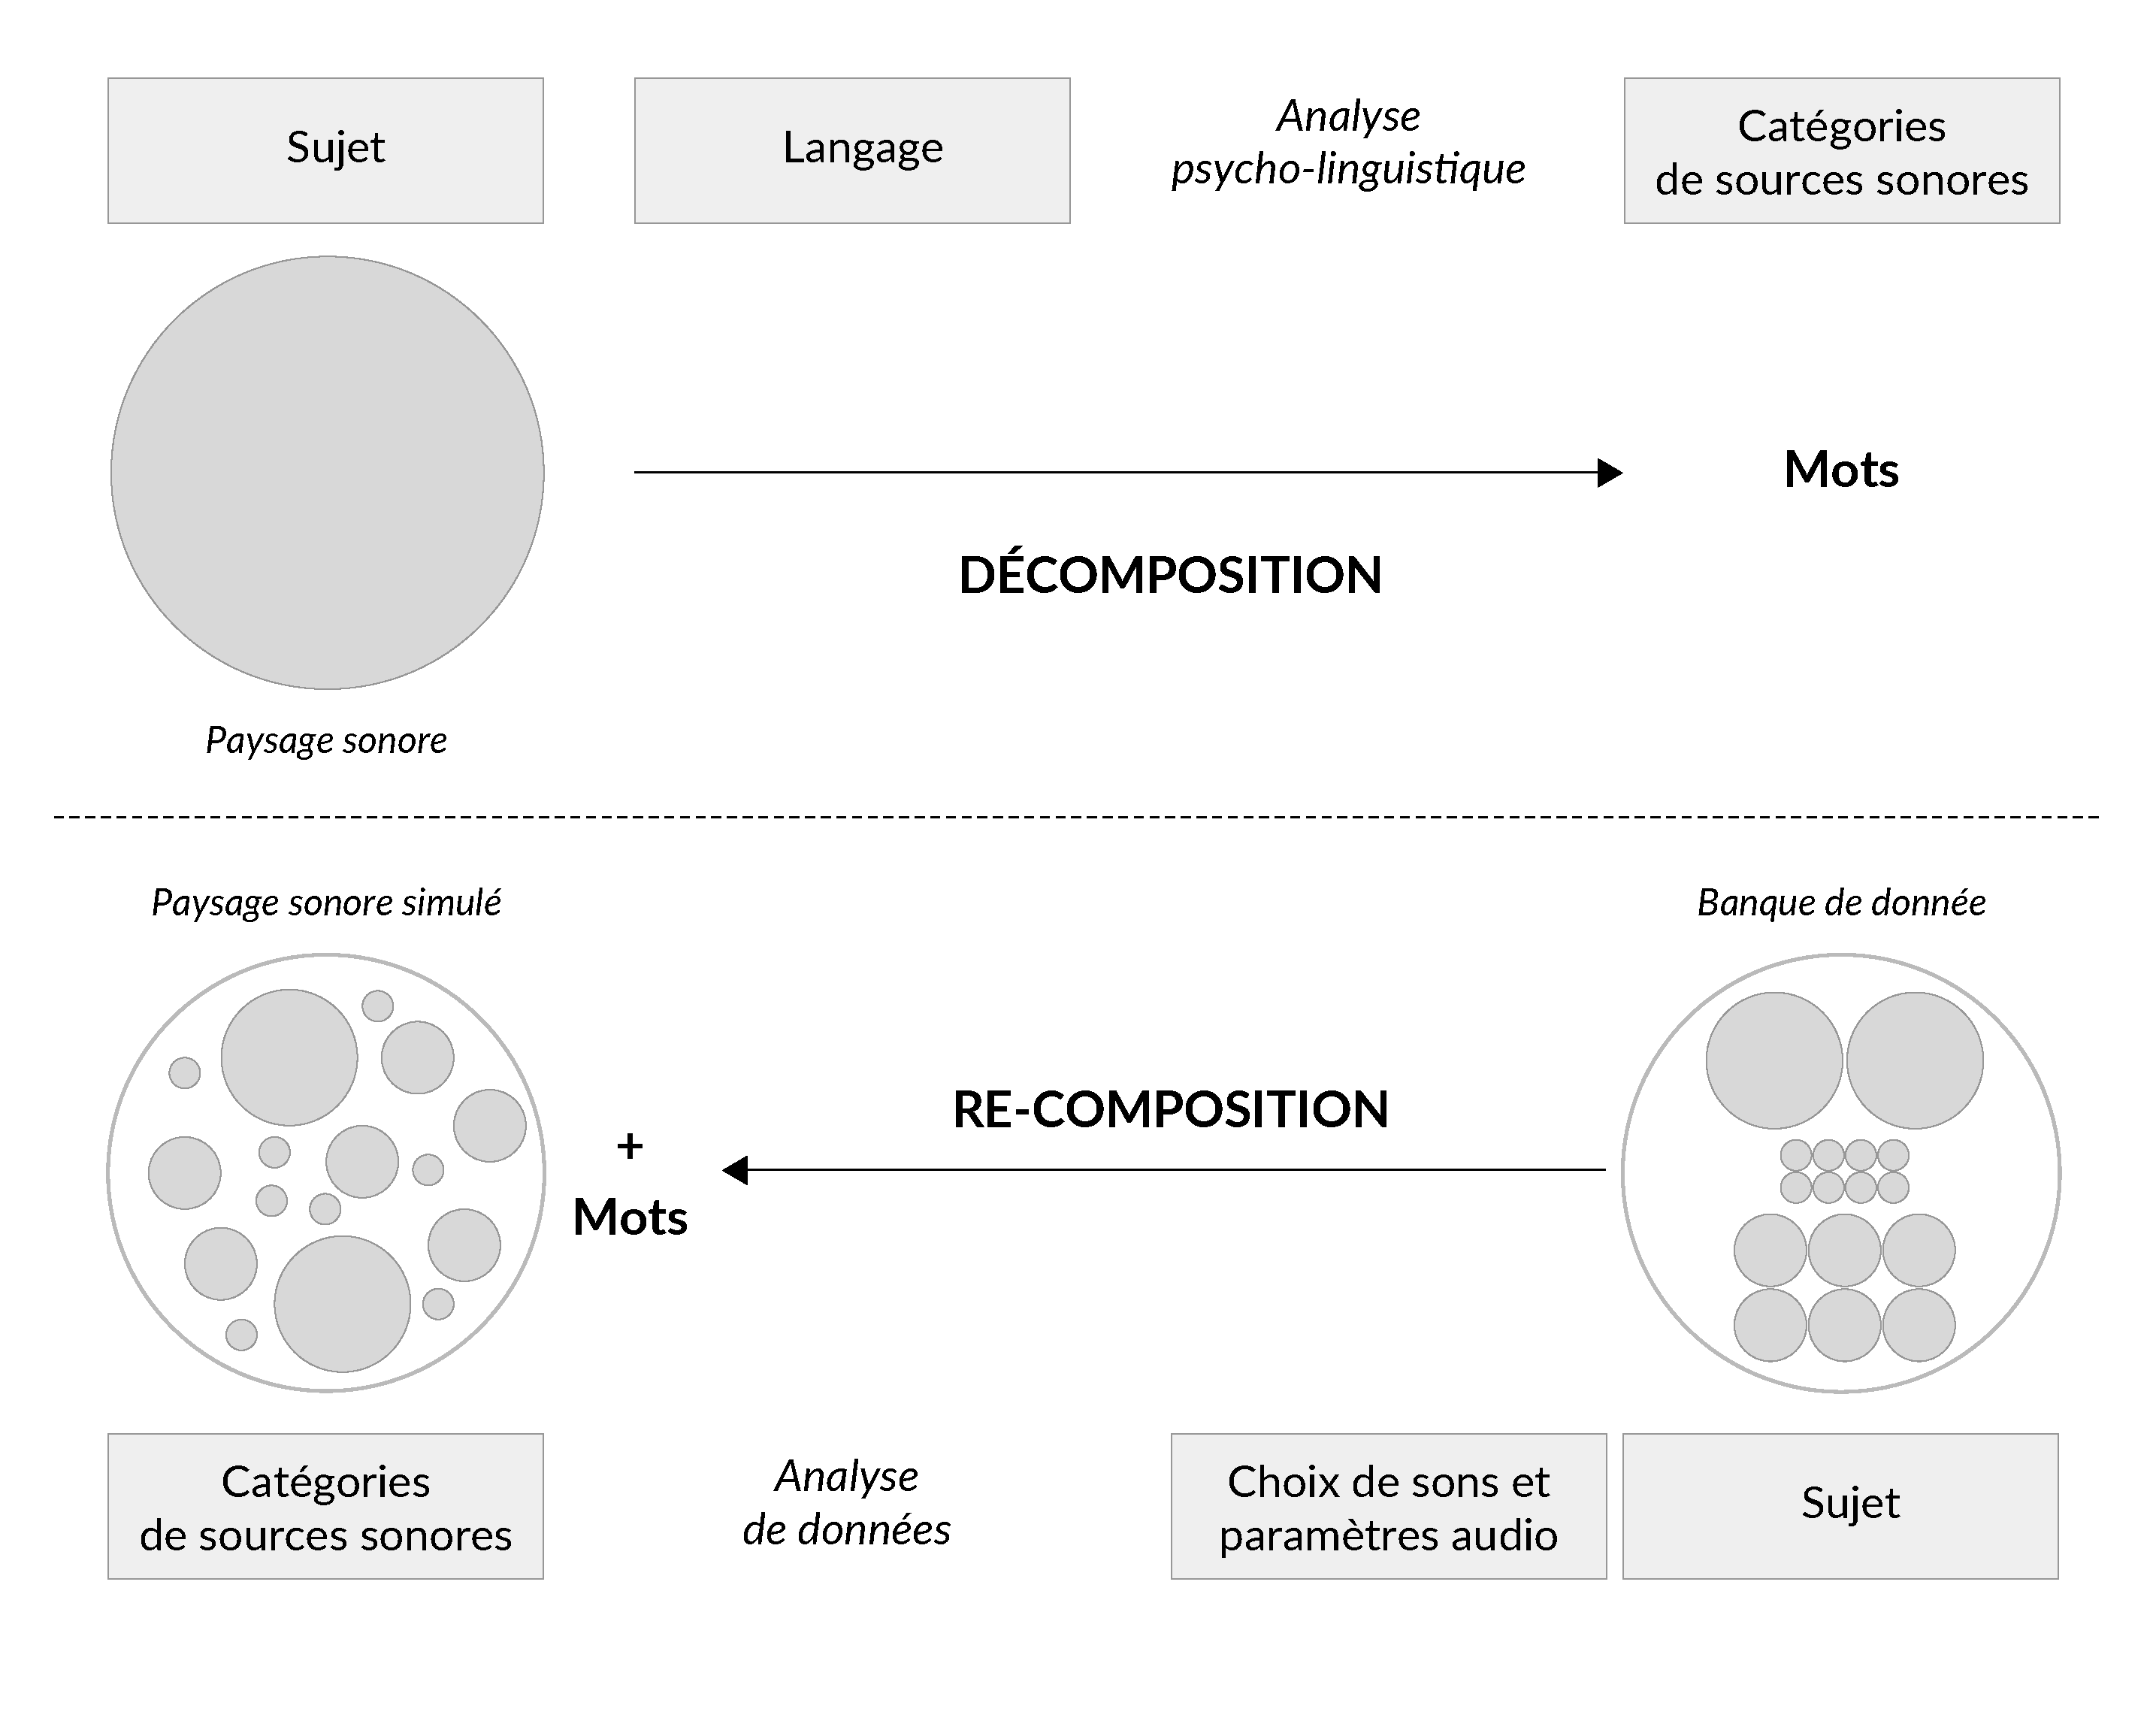
\includegraphics[width=.8\linewidth]{gfx/ch_4/1}
       \caption{TODO}\label{fig:paradigmeSimu1}
\end{figure}

\subsection{Analyse automatique}

\section{Proposition d'un modèle de scènes sonores}
\label{sec:ch4_model}

\subsection{Discrétiser l'environnement sonore}
\label{sec:ch4_modelInspi}


\subsubsection{L'unité de bases: la source sonore}

Les études portant sur l'ASA, et plus spécifiquement sur les processus de ségrégation, montrent, d'une part, que l'humain fait sens de son environnement en isolant les informations relatives aux différentes sources qui le composent, d'autre part, que ce groupement intervient très tôt dans la chaîne de traitement, et se base sur des règles génériques innées.\\

\gl{TODO: Neuroscience} \\ 

Dans le même temps, la recherche sur les paysages sonores, adoptant l’approche catégorielle, met en évidence que les processus de catégorisation s'appuient également sur la composition sémantique des scènes, \ie~les sources sonores identifiées. 

Pour notre modèle, il apparaît fondé de considérer comme élément de base la source sonore. Comme vu précédemment (\cf~Section~\ref{sec:ch3_categoEtAbstract}), la notion de source sonore est variable, un même objet pouvant être reconnu suivant plusieurs degrés d'abstraction.

\subsubsection{Typologie: niveaux d'abstractions et nomenclature source-action}
\label{sec:ch4_sourceAction}

La constitution de banques de sons peuplant l'environnement urbain est incontournable. Avant d'acquérir ces sources, \ie~de les enregistrer, il est nécessaire de les identifier. Une démarche naïve consisterait alors à établir la liste exhaustive de toutes les classes de sources sonores composant l'environnement. Une telle approche soulèverait deux problèmes:

\begin{itemize}
\item une source sonore peut se décrire en fonction de plusieurs niveaux d'abstraction. Identifier et nommer sont des actions déterminées par notre représentation mentale du monde (\cf~Section~\ref{sec:ch3_representationMentale}). Cette représentation s'organise, entre autre, suivant l'axe vertical des niveaux d'abstraction sur lequel s'appuie notre travail de catégorisation. Ainsi, si deux individus entendent un même son de voiture, il est possible que le premier le nomme ``\,voiture\,'' et le deuxième ``\,moteur\,''. Le dénombrement de l'ensemble des sources pouvant être utilisées par le modèle doit prendre en compte ce fait. Ces sources doivent être regroupées en classes hiérarchisées, afin de bâtir une structure taxonomique;
\item il n'existe pas de taxonomie standardisée des sources sonores. C'est une tradition des sciences modernes de classer et nommer les éléments avant de les étudier. Dans les domaines de la faune ou de la flore, une observation longue et minutieuse des sujets d'étude a permis d'élaborer un système de classification (taxonomie), et ainsi d'organiser et trier les objets en fonction de leurs propriétés partagées. Elle a permis encore d'élaborer une terminologie précise des classes d'objets. Grâce à quoi, la Biologie est devenue une science, laquelle science, au passage, devait donner naissance à la théorie de l'évolution \citep{lecointre2006tree}. Dans le domaine du son (ainsi que dans celui des odeurs), en revanche, point de système de classification \citep{dubois2000categories,niessen2010categories}. Nous trouvons à cela deux explications:

\begin{itemize}
\item \emph{champ lexical limité}: l'identification et la description d'un son sont des processus subjectifs étroitement liés au langage (\cf~Section~\ref{sec:ch3_catLang}). Deux sujets appartenant à deux groupes sociaux différents n'utiliseront pas les mêmes mots pour décrire un même objet. Pour établir un système de classification, il faut prendre une décision quant à la définition des termes utilisés. Or, contrairement au domaine de la vision, où une terminologie de base pour décrire les objets (couleur, forme etc.) est globalement partagée, le champ lexical applicable aux phénomènes acoustiques est, d'une part, limité (durée, fréquence...) \citep{dubois2000categories}, d'autre part, emprunté, dans une large mesure, à d'autres domaines perceptifs. On parle ainsi de brillance, ou de rugosité de sons. La diversité des termes descriptifs, et l'absence de consensus sur ce qu'ils désignent, rend difficile l'élaboration d'une classification standardisée;
\item \emph{influence du contexte}: L'identification et la description d'un son sont dépendantes du contexte (\cf~Section~\ref{sec:ch3_categoEtContexte}), \ie~de la nature des sources cooccurrentes dans la scène \citep{ballas1987interpreting,niessen2008disambiguating,gygi2011incongruency}.
\end{itemize}
\end{itemize}

Il apparaît clairement que les classes de sons peuplant notre environnement doivent être organisées autour d'une taxonomie: un système de classes hiérarchisées. Cependant il y a un choix à faire quant à la manière de regrouper les sons à l'intérieur de cette taxonomie.

Comme vu à la section~\ref{sec:ch3_catSourceSoundScape}, plusieurs études ont montré que la catégorisation des sources sonores s'opère suivant des attributs sémantiques. Parmi ceux-ci, deux reviennent souvent:

\begin{itemize}
\item la source (agent, objet, fonction), \ie~l'objet émettant le son;
\item l'action, \ie~le mouvement physique à l'origine du son.
\end{itemize} 

Ces deux attributs fonctionnent de pair. S'inspirant de l'organisation catégorielle verticale à trois niveaux de Rosch (\cf~Section~\ref{sec:ch3_categoEtAbstract}), Guyot et al. \citep{guyot1997} proposent un système de catégorisation où les auditeurs identifient des groupements de sources abstraits, au niveau superordonné (``\,Bruit généré par une excitation mécanique\,''), des actions, au niveau de base (``\,gratter\,'',``\,frotter\,'') et des sources, au niveau subordonné (``\,vaisselle\,'',``\,stylo\,''). Reprenant à son tour ce système, \citep{houix_lexical_2012} montre que les sons sont catégorisés, en premier lieu, à partir du type de sources, et ensuite, seulement, à partir d'actions.

L'association source-action semble être une base sensée sur laquelle bâtir une taxonomie, dans laquelle les classes haut-niveaux sont des classes abstraites de sources sonores (``\,véhicule\,''), les classes intermédiaires, des classes de sources sonores (``\,voiture\,''), et les classes basses, des actions sonores (``\,passage\,''). Pour les classes de bas niveau, la perméabilité intra-classe est minimale.

Cette association source-action n'est cependant pas suffisante. Le choix des labels utilisés doit faire l'objet d'une sélection particulière. Ces labels doivent être génériques, compréhensibles, et décrire de manière non ambiguë les objets de la classe considérée. Afin de les choisir, il est possible de se référer aux travaux de Gaver \citep{gaver1993world}, qui propose une taxonomie phénoménologique des sons, aux travaux de Niessen~\al \citep{niessen2010categories} qui, sur la base d'une étude bibliographique de près de 35 publications, établit la liste des catégories sonores les plus utilisées, aux travaux de Salamon~\al \citep{Salamon14}, qui, partant des travaux de \citep{brown2011towards} et reprenant l'association source-action, élabore une taxonomie de sons urbains.

\subsubsection{événements, textures et scènes amorphes}
\label{sec:ch4_eventTextureAmorphe}

Nous avons montré que l'utilisation de la nomenclature basée sur l’association source-action nous permet de dénombrer et trier l'ensemble des sons présents dans l'environnement.

La question est alors, sur la base de la taxonomie établie, d'enregistrer, pour chacune des classes, un nombre de sons suffisant. Considérant des environnements denses comme la ville ou la forêt, cette approche pose des problèmes pratiques de faisabilité.

Afin de contourner le problème, on peut là encore s’appuyer sur des considérations perceptives pour établir, dans un contexte expérimental donné, quels sons requièrent d'être enregistrés séparément, et quels groupes de sons peuvent être enregistrés ensemble.

D'une part, tous les sons n'ont pas le même intérêt. Une voix humaine peut facilement être isolée du reste des sons concurrents \citep{carlyon2004brain}. Inversement, un fond sonore de trafic urbain est moins informatif que d'autres sons ponctuels et proches~\citep{southworth1969sonic}.

Maffiolo montre à ce sujet (\cf~Section~\ref{sec:ch3_catsoundscape}) l'existence de deux processus cognitifs distincts dont l'activation dépend de la nature des environnements: l'analyse holistique, s'agissant de scènes amorphes, \ie~sans événements apparents, et l'analyse descriptive (sur la base d'une information sémantique extraite à partir des événements connus), s'agissant de scènes événementielles, \ie~comportant des événements identifiables.

D'autre part, le cerveau a tendance à résumer l'information extraite, lorsqu'il détecte qu'une séquence n'est composée que d'un mélange de sons similaires, et que ces sons n'enrichissent pas l'information. Voir les travaux sur les textures sonores (\cf~Section~\ref{sec:ch3_eventTexture}). 

Ces résultats nous amènent à penser que les processus de ségrégation dépendent de la nature structurelle de l'environnement. Lorsque des événements émergent d'un environnement sonore, le cerveau traite l'information des différentes sources de manière séparée. Plusieurs flux auditifs sont ainsi générés \ie~un pour chaque séquence d'événements émis par la même source. A l'inverse, quand le cerveau ne parvient pas à isoler d'événement, la scène est traitée globalement, tous ces éléments étant agglomérés dans un même flux.

Ainsi, trois types de sons semblent pouvoir être isolés:

\begin{itemize}
\item {événement sonore}: un son ponctuel dont les caractéristiques physiques varient au cours du temps;
\item {texture sonore}: un son long dont les caractéristiques physiques restent stables au cours du temps, et analysé à partir de statistiques extraites d'une représentation temps-fréquence;
\item \emph{scène événementielle}: un son contenant une information sémantique élevée;
\item \emph{scène amorphe}: un son contenant une faible information sémantique.
\end{itemize}

Il est concevable qu'il existe des connexions entre les notions de textures/événements, et celles de scènes amorphes/événementielles.

Les séquences événementielles peuvent être vues comme des séquences composées soit uniquement d'événements, soit d'événements et de textures, la présence d'événements, porteurs d'une information plus riche, primant quant au choix du processus à mettre en œuvre

Les textures et les scènes amorphes sont traitées de manière holistique, à partir de propriétés acoustiques globales pour les scènes amorphes \citep{dubois2006cognitive,maffiolo_caracterisation_1999}, et sur la base d'une information résumée statistiquement pour les textures \citep{mcdermott2013summary}. Toutes deux portent une information limitée \citep{saint1995classification,nelken2013ear}. Cependant, les séquences amorphes sont spontanément décrites par les sujets comme des ``\,fonds sonores\,'' \citep{maffiolo_caracterisation_1999,guastavino2006ideal}, induisant qu'elles n'existent que grâce à un processus de construction de flux auditifs, alors que les textures sont des objets définis seulement sur la base de leur nature physique. Un exemple de texture souvent cité est le son du ``\,galop\,'', qui selon le contexte peut se retrouver au premier plan de la scène. 

Partant de là, il est possible d'assimiler une scène amorphe à une texture, ses caractéristiques physiques demeurant stables au cours du temps. De fait, nombre de scènes amorphes (``\,brouhaha de rue\,'', ``\,brouhaha de trafic\,'') sont citées comme textures \gl{TODO: citation}. Cependant, l'inverse, considérer une texture comme une scène amorphe, n'est pas forcément vrai.
 
Afin de limiter le nombre d'enregistrements nécessaires, il est donc possible d'enregistrer directement des mixtures de sons, à condition que ces dernières puissent être considérées comme des textures, la définition de cette dernière notion englobant les scènes amorphes. 

\subsection{Description du modèle morphologique}
\label{sec:ch4_modelDes}

\subsubsection{Classe et collection de samples}
\label{sec:ch4_collecSons}

Dans le modèle proposé, la scène sonore est vue comme une somme de sources sonores, ou autrement dit, ``\,un squelette d'événements sur un lit de textures\,'' \citep{nelken2013ear}. \gl{pas d'équivalence, faire un lien entre les deux}

D'un point de vue pratique, ces éléments sonores sont enregistrés. Ces éléments sont nommés des samples.
 
\begin{mydef}
Un sample est un enregistrement d'un son isolé, qu'il s'agisse d'un événement ou d'une texture.
\end{mydef}


Ces samples, regroupés en classes de sons hiérarchisées, forment une taxonomie. Un exemple est donné figure~\ref{fig:orgDb}. Les niveaux hiérarchiques de la taxonomie sont appelés niveaux d'abstraction. Les classes ayant un niveau d'abstraction élevé constituent un regroupement conceptuel de samples ayant potentiellement des caractéristiques variées (\eg~{Humain}). Plus le niveau de la classe est bas, plus le groupement est précis, regroupant des samples similaires (\eg~\emph{voix-adulte-cri}). 

\begin{mydef}
Une classe est une collection de samples, jugés perceptivement équivalents. Si le niveau d'abstraction d'une classe est tel que cette dernière possède des sous-classes, alors sa collection de samples est la somme des collections respectives de chacune des sous classes.
\end{mydef}

Les classes de niveau d'abstraction élevé sont nommées uniquement à l'aide de termes abstraits désignant, de manière globale, les samples qu'elles regroupent (\eg~\emph{transport}). Les classes de bas niveau utilisent la nomenclature source-action (\eg~\emph{voiture passe}). Quant aux classes du dernier niveau, elles correspondent à des collections de samples, par définition, équivalents les uns aux autres.

\subsubsection{Séquences de samples}
\label{sec:ch4_seqSample}

Chaque classe de sons, sélectionnée pour faire partie de la scène simulée, est liée à une piste. Cette piste est une séquence temporelle où sont positionnés les différents samples. Elle est la contrepartie simulée du flux auditif.

\begin{mydef}
Une piste est une séquence temporelle composée de samples appartenant à une même classe de sons.
\end{mydef}

La construction de la taxonomie (nombre de classes, nombre de niveaux d'abstraction), dépend, évidemment, de la tâche considérée. 

L'ensemble des pistes, ainsi que leurs paramètres, forment ce que nous appelons une partition.

\begin{mydef}
La partition désigne l'ensemble des propriétés des pistes composant une scène, à savoir, les classes de sons liées aux pistes, et leurs paramètres structurels (niveau, espacement, début et fin, \cf~Section~\ref{sec:ch4_modelParam}).
\end{mydef}

\begin{figure}[t]
        \myfloatalign
        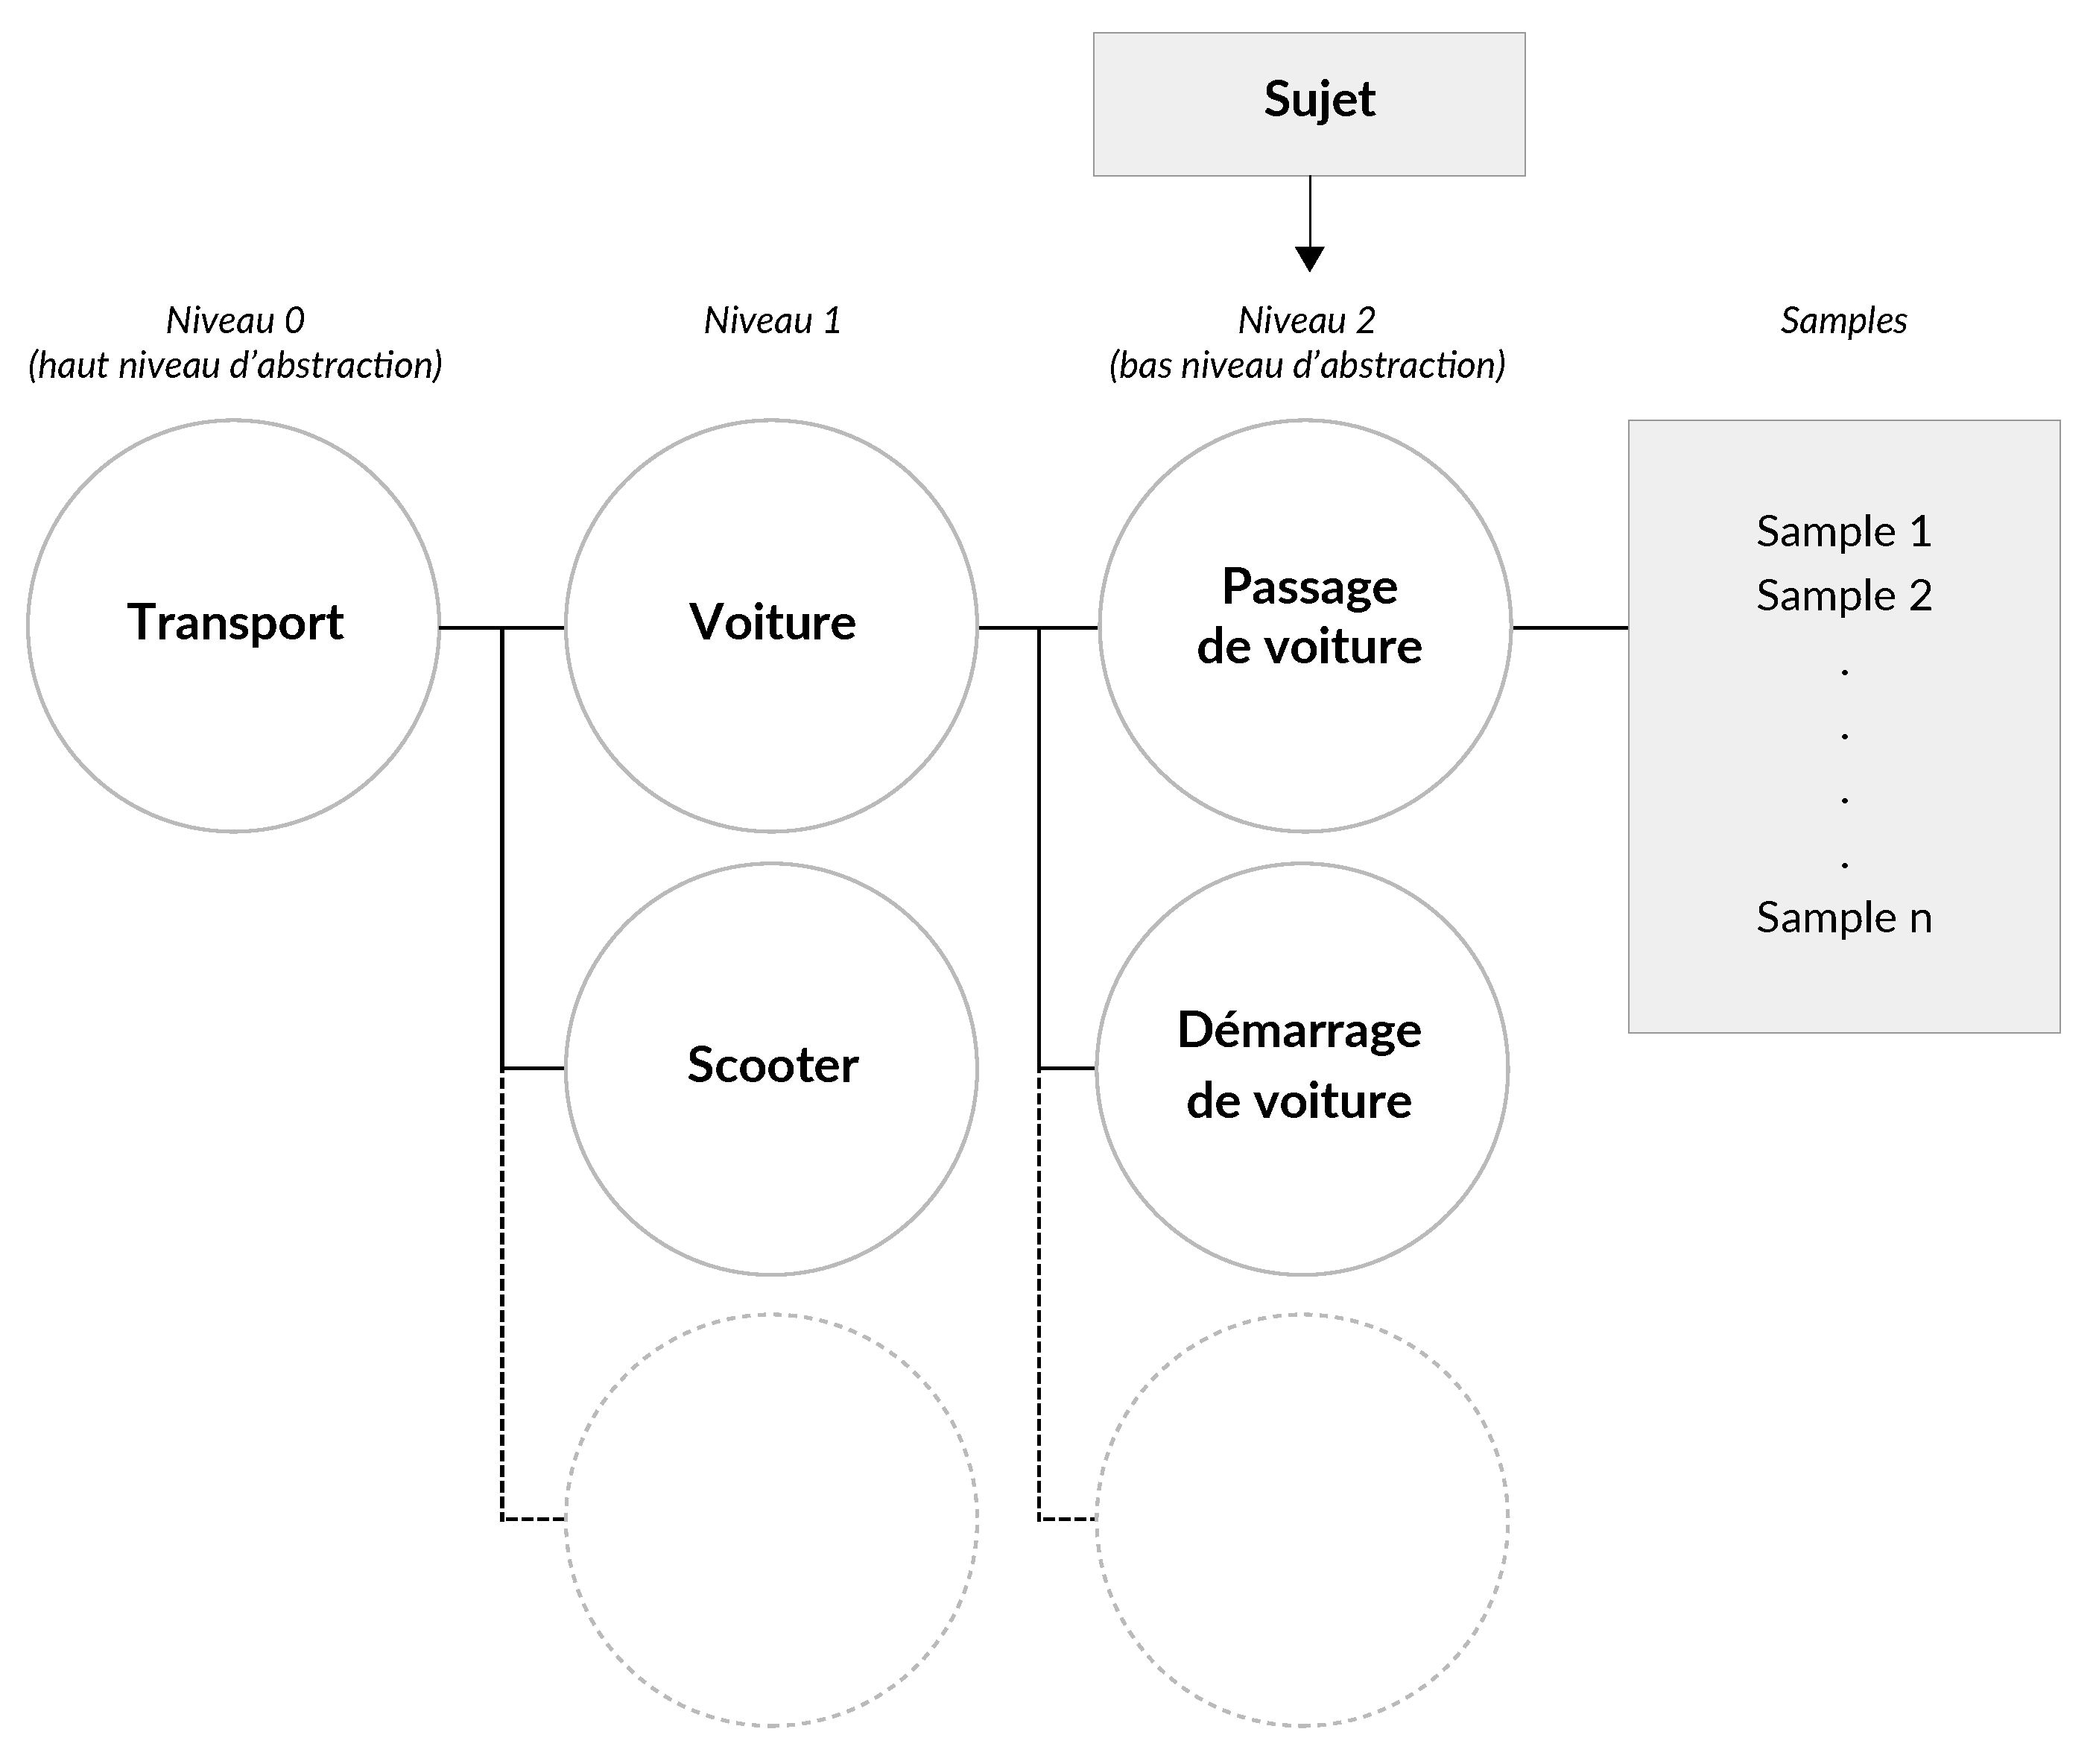
\includegraphics[width=.8\linewidth]{gfx/ch_4/3}
       \caption{Organisation hiérarchique de la banque de sons isolés utilisée pour la simulation}\label{fig:orgDb}
\end{figure}

\subsubsection{Paramètres}
\label{sec:ch4_modelParam}

En suivant la terminologie ci-devant introduite, une scène sonore est vue comme une somme de pistes. Chaque piste est une séquence temporelle, dont la structure dépend d'une série de paramètres (\cf~figure~\ref{fig:modelSequence}). Le modèle ne propose pas d’interagir avec un sample en particulier, mais toujours avec une séquence de samples.

Nous isolons trois attributs permettant de contrôler une piste:

\begin{itemize}
\item \emph{niveau}: la moyenne/variance des niveaux des samples;
\item \emph{espacement}: la moyenne/variance des espacements inter-\emph{onsets} entre les samples;
\item \emph{durée}: le début et la fin de la piste.
\end{itemize}

Le modèle fait une distinction explicite entre la gestion des pistes d'événements, et la gestion des pistes de textures. En effet, la notion de texture ne peut se comprendre que pour un son continu. Une piste de texture est donc composée de samples concaténés les uns aux autres, sans espacement (\cf~figure~\ref{fig:modelSequence}). 

Pour qu'une piste de texture soit ``\,plausible\,'', \ie~qu'on ne détecte pas de discontinuité flagrante, elle doit être une séquence composée de samples provenant de la même source, et obtenus avec un matériel (et des réglages) identique(s).

\begin{figure}[t]
        \graphicspath{{gfx/ch_4/}}
        \myfloatalign
        \def\svgwidth{\linewidth}
        \input{gfx/ch_4/controlParameters2.pdf_tex}
       \caption{TODO}\label{fig:modelSequence}
\end{figure}

\subsubsection{Formalisation du modèle}
 \label{sec:ch4_modelForm}
 
 Tout au long de nos travaux, nous avons utilisé plusieurs modèles, ainsi que différents paramètres, afin de simuler des scènes sonores. Nous formalisons, dans cette partie, une version générale du modèle proposé. Les diverses modifications appliquées au modèle, en fonction de son utilisation, sont indiquées dans les sections~\ref{sec:ch4_modAnaSo} et~\ref{sec:ch4_modAnaAuto}.
 
La formalisation présentée vaut uniquement pour les classes d'événements sonores. Nous décrivons par la suite les diverses contraintes qui s'appliquent pour une classe de textures.
 
En considérant $s$, une scène composée de $z$ classes de sons, le modèle de $s$ se définit comme suit:
 
 \begin{equation}
 s(n)=\sum_{i=1}^{z}p_i(n)
 \end{equation}

avec $n$ un indice temporel discret, et $p_i$ la piste correspondant à la classe $c_i$. La classe $c_i$ est composée de $\vert c_i\vert$ samples $c_{i,m}$, $1<m<\vert c_i\vert$. 

Une piste $p_i$ est définie comme une séquence de $n_i$ samples d'événements $e^k_i(n)$ ($k=(1,2,\ldots,n_i)$), choisis aléatoirement parmi les $\vert c_i\vert$ samples de la classe $c_i$. Considérant $\mathcal{U}(x,y)$, une distribution uniforme d'entiers allant de $x$ à $y$ ($x<y$), on a alors:

 \begin{equation}
 e^k_i=c_{i,\mathcal{U}(1,\vert c_i \vert)}
 \end{equation}

 Pour chaque piste $p_i$, un facteur d'amplitude est tiré aléatoirement à partir d'une distribution normale de moyenne $\mu^a_i$ et de variance $\sigma^a_i$. De même, les espacements inter-\emph{onsets} sont tirés d'une distribution normale de moyenne $\mu^t_i$ et de variance $\sigma^t_i$. Les indices temporels de début et de fin de chaque piste sont notés $u_i$ et $v_i$ respectivement. Formellement, une piste $p_i$ se définit comme suit:
 
\begin{equation}
\label{eq:ch4_eq1}
p_{i}(n)= \sum_{j=1}^{n_i} \mathcal{N}(\mu^a_{i},\sigma^a_{i})c_{i, \mathcal{U} (1, |c_i|)}(n-n^j_i)
\end{equation}
\begin{equation}
\label{eq:ch4_eq2}
n_i^j=n_i^{j-1} + \mathcal{N}({\mu^t_{i},\sigma^t_{i}})
\end{equation}

où $n_i^0=u_i$ par convention. Le signal d'une piste est défini de telle sorte que $p_i(n)=0$ si $n>v_i$. Les paramètres du modèle sont, $\mu^a_i$,  $\sigma^a_i$,   $\mu^t_i$,  $\sigma^t_i$, $u_i$ et $v_i$, et doivent être réglés pour chaque piste $p_i$. La figure~\ref{fig:modelSequence} offre une illustration de l'action des paramètres introduits.


Pour les textures, deux distinctions sont à observer avec le modèle défini précédemment: 

\begin{enumerate}
\item l'amplitude du signal ($\mu^a_i$,  $\sigma^a_i$) n'est tirée qu'une seule fois, et la valeur est appliquée à tous les samples;
\item afin d'éviter toute sensation de discontinuité, deux samples de texture sont concaténés en considérant un recouvrement fixé, sur lequel est appliqué un fondu enchaîné (\emph{cross-fade}) à valeur d'énergie constante entre les samples, afin de donner l'illusion de continuité.
\end{enumerate}

\gl{TODO: à revoir avec mathieu et mathias}

\section{Du modèle à la simulation: l'analyse sensorielle}
\label{sec:ch4_modAnaSo}

Dans cette section nous présentons une version du modèle précédemment introduit, afin qu'il puisse servir de base à un outils de simulation, nommé \emph{SimScene}, utilisable dans le cadre de l'analyse sensorielle des scènes sonores.

Nous commençons par présenter différents outils existant, permettant de simuler des environnements sonores. Nous proposons, par la suite, un protocole expérimental, décrivant le cadre applicatif des épreuves perceptives basées sur la simulation. Enfin, nous relions ce protocole au modèle de scènes sonores (\cf~Section~\ref{sec:ch4_modelParam}), et présentons les fonctionnalités de l'outil \emph{SimScene}.

\subsection{Simulation et analyse sensorielle}

Plusieurs outils de simulation de scènes sonores ont déjà été proposés \citep{misra2006new,misra2007musical,valle2009framework,finney2010soundscape,schirosa2010system}. Ils ont souvent pour but de générer automatiquement l'ambiance sonore d'un environnement virtuel. \citep{valle2009framework,finney2010soundscape}. Ils peuvent être vus comme des systèmes semi-autonomes: la simulation pouvant être contrôlée par un utilisateur, mais dépendant aussi, soit d'un environnement visuel à illustrer, soit d'un environnement sonore à reproduire. D'autre outils, entièrement contrôlés par un utilisateur, servent, eux, d'aide à la composition \citep{misra2006new,misra2007musical}. Ces systèmes s'éloignent tous sensiblement du cadre expérimental de l'analyse sensorielle.

A notre connaissance, seuls Bruce~\al \citep{bruce2009development,bruce2014effects} se sont servis de la simulation afin d'étudier la perception des paysages sonores. Ils proposent un système permettant au sujet d'agir sur un environnement en ajoutant ou supprimant des sources sonores spécifiques. Celui-ci peut par ailleurs modifier le niveau sonore des sources, et leurs positions spatiales.

A l'aide de cet outil, les auteurs demandent à leurs sujets de manipuler des sources, afin de recréer un environnement urbain. Les résultats montrent que l'inclusion ou l'exclusion des sources dépend plus de considérations sociales/sémantiques, que des caractéristiques physiques des sources. Ils soulignent néanmoins que le manque d'enregistrements disponibles limite l'analyse. Ils suggèrent de regrouper les enregistrements similaires en ``\,groupes sémantiques\,'' afin de faciliter l'analyse. \\

\gl{TODO G1: compléter Bruce~\al, cf wac} \\
\gl{TODO G2: \citep{davies2014soundscape} montre que, lorsqu'on demande à des participants de simuler un paysage sonore, les simulations font références à ce que ces derniers s'imaginent être un environnement typique, sans tenir compte de leur propre préférence pour des sons particuliers.}

\subsection{Protocole expérimental basé sur la simulation}

\subsubsection{Organisation des sons isolées}
\label{sec:ch4_dbEventTexture}

L'objectif de l'expérimentation est de permettre à un sujet de simuler un environnement sonore cible, à partir de sons isolés. La banque de sons suit l'organisation décrite à la section~\ref{sec:ch4_collecSons}. Les éléments sont regroupés en classes hiérarchisées, afin de former une taxonomie. Plus le niveau d'abstraction de la classe est élevé, plus la variabilité des enregistrements appartenant à la classe est importante (\cf~Figure~\ref{fig:orgDb}).
 
Nous conservons la distinction observée entre les événements et les textures, en créant deux taxonomies (\ie~deux banques de sons) séparées.

\subsubsection{Sélection des sons isolées}

L'objectif de la simulation est d'obtenir une image sonore de la représentation mentale que ce fait un sujet d'un environnement donné. Afin que cette image soit la plus ``\,juste\,'' possible, il faut que le protocole limite les biais pouvant influer sur les choix du sujet.

Un de ces biais intervient dans le processus de sélection. La grande majorité des outils permettant de parcourir une banque de données propose une recherche textuelle sur la base de mots clefs. L’efficacité de ce principe repose avant tout sur la structure typologique, et la nomenclature de la base de données. Dans le cadre d'une expérience sensorielle visant à objectiver une représentation interne d'un sujet, cette approche pose trois problèmes majeurs :

\begin{itemize}
\item les sons peuvent ne pas être tagués d'une manière satisfaisante. En effet, sémantiquement, un son peut être décrit de plusieurs façons. Nous pouvons en désigner la source (une portière de voiture), comme nous pouvons désigner l'action de la source (le claquement d’une portière de voiture) ou encore son environnement (le claquement d’une portière de voiture dans un garage). Concevoir un système de recherche par mots clefs efficace suppose une description précise de chaque son, qui plus est adaptable à la représentation que s’en fait chaque sujet, ce qui est difficilement réalisable;

\item lors d'une recherche par mots clefs, le sujet doit objectiver un nom décrivant l'objet recherché. Or cette objectivation dépend des connaissances collectives du sujet, connaissances liées à sa sphère socioculturelle, et en particulier à sa langue. L'expérience visant une diffusion internationale, cette contrainte est difficilement surmontable;

\item la description verbale du son, si elle est accessible par le sujet, peut potentiellement influencer sa sélection. Dans les faits, pour construire une scène environnementale ``\,calme\,'', le sujet sélectionne a priori les sons référencés sous le vocable \emph{parc}. Cette réalité constitue encore une difficulté.
\end{itemize}

Imposer au sujet une terminologie \gl{à travers les labels} décrivant les classes est un risque. La sélection doit s'éloigner le plus possible d'un ancrage sémantique, et s'effectuer à l'aveugle, \ie~sur la base uniquement de l'écoute. Une interface développée spécialement dans ce but est présentée à la section~\ref{sec:ch4_ssf}.

Enfin, il est important de noter que le sujet ne peut accéder qu'aux classes du niveau d'abstraction le plus bas, classes qui ne possèdent pas de sous-classes, et sont directement liées à une collection de samples.

L’organisation hiérarchique sert alors deux buts:

\begin{itemize}
\item faciliter le parcours, par les sujets, des banques de sons isolées (\cf~Section~\ref{sec:ch4_ssf});
\item faciliter le travail d'analyse de l'expérimentateur, en lui permettant d'observer la composition en terme de sources sonores des scènes, suivant différents niveaux d'abstraction.
\end{itemize}

\subsubsection{Processus de simulation}
\label{sec:ch4_processSimu}

\begin{figure}[t]
        \myfloatalign
        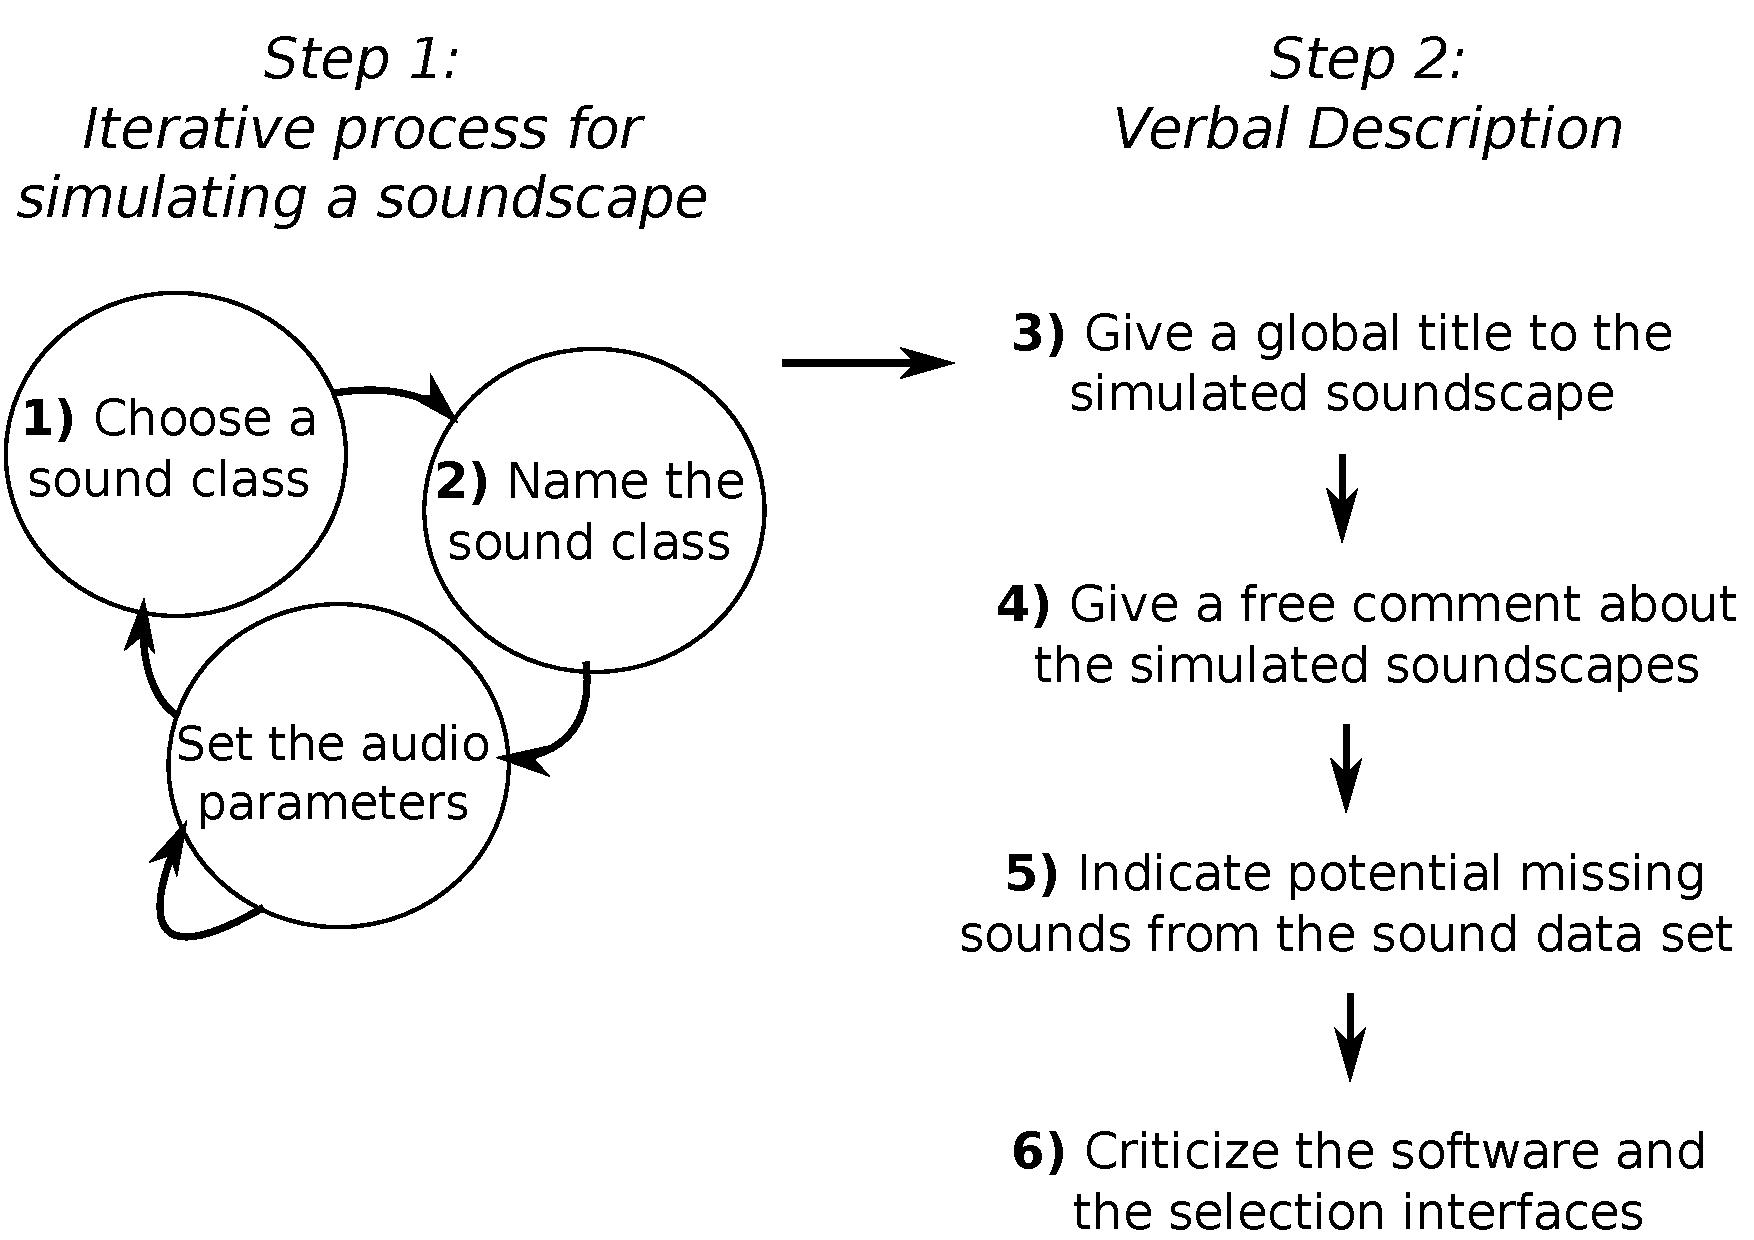
\includegraphics[width=.8\linewidth]{gfx/ch_4/4}
       \caption{Etape de processus de simulation pour l'analyse sensorielle}\label{fig:etapeSimu}
\end{figure}

Trois étapes composent le processus de simulation (\cf~Figure~\ref{fig:etapeSimu}):

\begin{itemize}
\item \emph{sélection} d'une classe de sons. Une fois une classe sélectionnée, une piste est générée; 
\item \emph{identification} de la classe de sons sélectionnée. Le sujet nomme la classe de sons qu'il a sélectionnée;
\item \emph{paramétrisation} de la piste liée à la classe de sons. Le sujet fixe les paramètres de la piste (pour plus de détails sur les paramètres proposés \cf~Section~\ref{sec:ch4_param}).
\end{itemize}

Ces étapes peuvent être répétées, et dans n'importe quel ordre, le sujet pouvant agir rétrospectivement sur les pistes déjà crées. A la fin de la simulation, et afin d'accumuler le maximum de connaissances possible sur la scène simulée, le sujet peut: 

\begin{itemize}
\item nommer l'environnement simulé;
\item fournir un commentaire libre décrivant son processus de création, ainsi que le paysage sonore qu'il a voulu illustrer.
\end{itemize}

\subsection{Paramètres de contrôle}
\label{sec:ch4_param}

Les paramètres du modèle permettent au sujet de contrôler la structure de chaque piste. Ils agissent sur tous les samples à la fois, et non sur un en particulier.

Parmi ces paramètres, on retrouve ceux introduits pour le modèle initial de scène sonore (\cf~Section~\ref{sec:ch4_modelParam} et~\ref{sec:ch4_modelForm}), à savoir:

\begin{itemize}
\item \emph{niveau sonore} ($dB$): pour chaque sample, les niveaux sont tirés aléatoirement à partir d'une distribution normale, paramétrée par le sujet en terme de moyenne et variance;
\item \emph{espacement inter-onset} (seconde): (piste d'événements seulement) comme pour les niveaux, les espacements sont tirés aléatoirement à partir d'une distribution normale, paramétrée par le sujet en terme de moyenne et variance;
\item \emph{début et fin} (seconde): le sujet fixe le début et la fin de chaque piste.
\end{itemize}

Afin de faciliter la simulation, deux paramètres supplémentaires sont proposés:

\begin{itemize}
\item \emph{fondu par événement} (seconde): (piste d'événements seulement) le sujet fixe une durée de fondu (entrée et sortie), appliquée à chaque sample d'une piste d'événements;
\item \emph{fondu global} (seconde): le sujet fixe les durées de fondus séparément, pour l'entrée et la sortie de la piste. Ces fondus s'appliquent ainsi à l'ensemble des samples de la piste.
\end{itemize}

Deux de ces paramètres ne s’appliquent que pour les pistes d'événements (\emph{fondu par événement} et \emph{espacement inter-onset}), les samples des textures étant séquencés sans espacement (\cf~Section~\ref{sec:ch4_modelParam})

\subsubsection{Données produites par le processus de simulation}

\begin{figure}[t]
        \myfloatalign
        \includegraphics[width=.8\linewidth]{gfx/ch_4/schemaXP}
       \caption{TODO}\label{fig:paradigmeSimu2}
\end{figure}

Ce protocole de simulation peut potentiellement produire un grand nombre de données. Ces dernières sont décrites à la figure~\ref{fig:paradigmeSimu2}.  Nous les résumons dans la liste suivante:

\begin{itemize}
\item données sémantiques objectives: la banque de données nous permet d'obtenir une information objective quant aux sources sonores présentes dans la scène. Les données sémantiques objectives sont les labels des classes sélectionnées;
\item données sémantiques subjectives: il s'agit des noms donnés par le sujet 1) à la scène simulée, 2) aux classes de sons sélectionnées;
\item données quantitatives issues de la partition: il s'agit de toutes les données relatives à la partition, \ie~pour chaque piste, le positionnement des samples et les paramètres (\cf~Section~\ref{sec:ch4_seqSample});
\item données quantitatives issues du signal: il s'agit d'indicateurs acoustiques extraits du signal, \eg~le niveau sonore global. Comme nous possédons les samples isolés utilisés pour la synthèse, il est possible de calculer ces descripteurs pour une classe, ou un ensemble de classes, en particulier.
\end{itemize}

Le protocole nous permet de caractériser avec précision une scène simulée, sur la base de données sémantiques, subjectives ou objectives, ainsi que quantitatives. Considérant l'ensemble des données générées, les potentiels d'analyse sont vastes.



\subsection{Interface de sélection aveugle des sons isolés}
\label{sec:ch4_ssf}

\begin{figure}[t]
        \myfloatalign
        \includegraphics[width=.8\linewidth]{gfx/ch_4/SSF}
       \caption{L'interface de sélection aveugle de l'outil de simulation \emph{Simscene}}\label{fig:ssf}
\end{figure}

Pour limiter l’influence de l’interface sur le sujet, il nous paraît nécessaire de libérer sa recherche de toute information textuelle. Nous proposons à l'utilisateur une interface graphique lui permettant d’explorer la banque de sons exclusivement à partir de l’écoute.

Visuellement, les classes du dernier niveau (les seules accessibles par le sujet) sont représentées par des cercles, et positionnées sur un plan. La disposition des cercles dans l'espace dépend de l’organisation hiérarchique de la base de données: les sous-classes appartenant à la même classe sont proches les unes des autres, et ainsi de suite jusqu'à atteindre les classes des niveaux d'abstraction élevés.

La figure~\ref{fig:ssf} présente l'interface pour la banque de données d'événements sonores. Cette organisation visuelle à été pensée afin de:

\begin{enumerate}
\item faciliter le parcours de la banque de données, les sons similaires (au sens des classes) étant proches les uns des autres. L'organisation hiérarchique se fonde, en effet, sur des principes cognitifs. Les classes ont été établies à partir de la littérature traitant des catégories de sources sonores (\cf~Section~\ref{sec:ch4_collecSons}).
\item permettre aux sujets de rapidement appréhender toute l'étendue de la banque de données, \ie~l'ensemble des sons disponibles.
\end{enumerate}

Chaque classe possède un son prototype. Ces sons ont été choisis par les expérimentateurs. Lorsqu’on ``\,clique\,'' sur un cercle, le prototype associé à la classe est joué. Le sujet parcours la banque de sons en cliquant sur les cercles.

Cette interface a fait l'objet d'une étude approfondie dont les résultats sont publiés dans \citep{lafay2016JAES}. \\

\gl{TODO: résumer les résultats JAES}

\subsection{Interface de simulation: l'outil \emph{Simscene}}
\label{sec:ch4_simscene}

\begin{figure}[t]
        \myfloatalign
        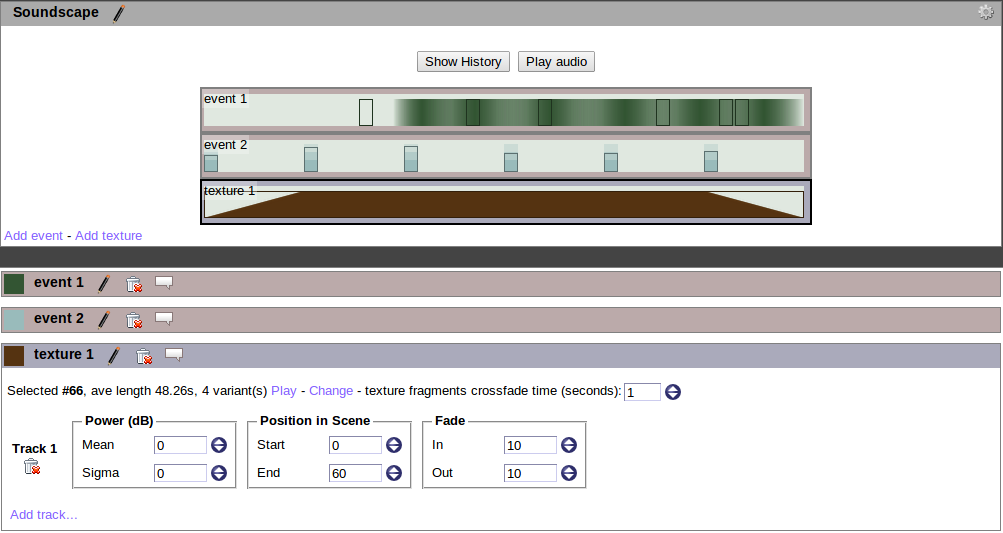
\includegraphics[width=.8\linewidth]{gfx/ch_4/simscene}
       \caption{L'outil de simulation \emph{Simscene}}\label{fig:simscene}
\end{figure}

\emph{Simscene} est un environnement de travail audio-numérique, supporté par navigateur internet, et développé dans le cadre du projet HOULE\footnote{Pour plus d’informations sur le Projet HOULE voir \url{http://houle.ircam.fr/}}. Il permet de simuler des paysages sonores à partir d'un corpus de sons. Il est prévu pour fonctionner via les navigateurs internet \emph{Chrome} et \emph{Firefox}. L'outil a été développé en javascript à l'aide de la bibliothèque \emph{angular.js}\footnote{\emph{angular.js}: \cf~\url{https://angularjs.org/}} et du standard \emph{web-audio}\footnote{\emph{web-audio}: \cf~\url{http://www.w3.org/TR/webaudio/}}. L'interface de sélection (\cf~Section~\ref{sec:ch4_ssf}) a été développée à l'aide de la bibliothèque \emph{D3.js} \citep{d32011}.

\emph{Simscene} est présenté en détail dans \citep{rossignol2015simscene}. \gl{Nous résumons ici ses fonctionnalités d'importance pour notre étude}. 

Le fonctionnement de \emph{Simscene} se rapproche de celui d'un séquenceur audio. Chaque utilisateur choisit une classe de sons via l'interface de sélection (\cf~Section~\ref{sec:ch4_ssf}). Une fois la classe de sons sélectionnée, une piste audio, liée à cette classe, est créée. L'utilisateur peut alors modifier certaines propriétés de la piste via un groupe de paramètres de contrôle propre à chacune (\cf~Section~\ref{sec:ch4_param}). Des champs de texte sont prévus afin de permettre à l'utilisateur de 1) nommer chaque piste, 2) donner un titre à la scène simulée et 3) commenter la scène simulée.

L'interface propose un rendu graphique schématisé de la scène en cours de création (\cf~Figure~\ref{fig:simscene}). La piste est représentée par une bande possédant un axe temporel. Sur cette bande, chaque sample est représenté par un rectangle. L'espacement entre les rectangles est relatif à l'espacement entre les samples. De même, la hauteur des rectangles est proportionnelle au niveau sonore des samples. Dans le cas d'une piste de texture, un unique rectangle apparaît sur toute la longueur de la piste, un son de texture ne pouvant être entrecoupé de silences. Les caractéristiques des rectangles évoluent en fonction des changements de paramètres de la piste.

L'utilisateur a la possibilité, à tout moment, d'écouter la scène simulée.

L'outil de simulation est accessible via le lien suivant: \url{http://www.irccyn.ec-nantes.fr/~lagrange/
demonstrations/simScene.html}

\section{Du modèle à la simulation: l'analyse automatique}
\label{sec:ch4_modAnaAuto}

Un ensemble dédié de fonctions Matlab, qui sont accessibles au public\footnote{https://bitbucket.org/mlagrange/simscene/downloads}.
%*****************************************
%*****************************************
%*****************************************
%*****************************************
%*****************************************

%************************************************
\chapter[Application du modèle à l'analyse sensorielle]{Application du modèle morphologique à l'analyse sensorielle des scènes sonores environnementales urbaines}\label{ch:psycho_xp}
%************************************************

\gl{TODO: concernant le titre: pourquoi modèle morphologique plus que "simulateur" ? il manque le coté "création" dans modèle morphologique}

\section{Introduction}

Comme nous l'avons vu (\cf~Section~\ref{sec:ch3_contribSource}), la recherche sur les paysages sonores a besoin d'outils permettant d'analyser les influences séparées des différentes sources sur les qualités affectives de l'environnement. La simulation offre des possibilités intéressantes (\cf~Section~\ref{sec:ch4_anaSo}), car elle nous permet d'obtenir des scènes sonores dont nous connaissons tous les paramètres structuraux, en particulier les caractéristiques distinctes des différentes sources. 
 
Afin de montrer les potentialités inhérentes à l'utilisation de scènes simulées en analyse sensorielle, nous choisissons, comme cadre applicatif, le problème de l'agrément perçu dans les environnements sonores urbains. 

Cette section présente les résultats d'une série de quatre expériences visant, chacune, à comprendre comment les différentes sources sonores qui composent une scène influent sur la perception de l'agrément. Toutes ses expériences s'appuient sur la simulation. La première est l'expérience de simulation à proprement parler, \ie~où les sujets doivent créer les environnements. Les autres sont des épreuves de notation ou de tri classiques, utilisant les scènes simulées comme stimuli:

\begin{enumerate}
\item \emph{expérience de simulation}: au cours de cette expérience, chaque sujet doit simuler deux environnements sonores urbains, le premier idéal/agréable et le deuxième non-idéal/désagréable, en utilisant l'outil et le protocole de simulation décrits à la section~\ref{sec:ch4_simscene};
\item \emph{évaluation de l'agrément}: les sujets doivent évaluer l'agrément des scènes simulées à partir d'une échelle sémantique;
\item \emph{évaluation de l'agrément après modification des scènes}: comme pour l'expérience précédente, les sujets doivent évaluer l'agrément des scènes simulées à partir d'une échelle sémantique. Cependant les scènes ont été modifiées, \ie~privées de certaines classes de sons identifiées comme ayant un impact sur l'agrément perçu; 
\item \emph{catégorisation libre}: les sujets doivent catégoriser les scènes sonores simulées. Au delà du problème initial de l'agrément, cette dernière expérience nous amène à considérer logiquement l'influence de la composition sémantique des scènes sur les jugements de similarités.
\end{enumerate}

Les expériences 1 et 2 vont de pair, et sont toutes deux décrites dans la section~\ref{sec:xp1_2}. Les expériences 3 et 4 sont, elles, décrites respectivement dans les sections~\ref{sec:xp3} et~\ref{sec:xp4}  \\

Tout au long de la présentation de ces expériences et de leurs résultats, nous poursuivrons deux objectifs:

\begin{itemize}
\item \emph{objectif méthodologique}: montrer les possibilités offertes par l'utilisation de scènes simulées dont nous connaissons précisément la partition (\cf~Section~\ref{sec:ch4_modelDes}) dans le cadre d'études sensorielles ayant trait à la perception des sons;
\item \emph{objectif applicatif}: étudier quels sont les éléments qui participent à la perception de l'agrément dans les environnements sonores urbains. 
\end{itemize}

\section[Agrément perçu et composition sémantique]{L'impact de la composition sémantique des scènes sur la perception de l'agrément}
\label{sec:xp1_2}

\subsection{Objectif}

L'objectif est d'étudier les influences spécifiques des différentes sources sonores qui composent les environnements urbains, sur la perception de l'agrément, en utilisant la simulation. Pour ce faire, nous planifions nos deux premières expériences (\cf~Figure~\ref{fig:xp1_2}):

\begin{itemize}
\item \emph{expérience de simulation}: comme précisé auparavant, au cours de cette expérience, les sujets simulent les environnements qui serviront de stimuli pour les étapes suivantes. Chaque sujet compose deux scènes opposées, les premières répondant à la description idéales/agréables (i-scènes), les secondes répondant à la description non idéales/désagréables. Cette épreuve de simulation a fait l'objet d'une expérience pilote \citep{lafay2013atiam,lafay2014new}; \gl{TODO: préciser xp pilote}
\item \emph{expérience d'évaluation}: a l'issue de la simulation, nous n'avons, de fait, qu'une connaissance binaire des propriétés affectives des scènes simulées: idéale (i) et non-idéale (ni). Cette seconde étape a pour but d'affiner notre connaissance sur l'agrément de chacune des scènes. Pour ce faire, nous demandons à un deuxième groupe de sujets d'évaluer, à partir d'une échelle sémantique, l'agrément de chacune des scènes simulées. L'expérience d'évaluation sert deux buts:
\begin{enumerate}
\item évaluer l'influence des différentes sources sur l'agrément perçu, de manière séparée, pour chaque type d'environnement (i ou ni);
\item détecter la présence de cas extrêmes ou ambigus (\emph{outlier}) dans les scènes simulées. Pour le reste de notre étude, les qualités hédoniques imposées (i et ni) servent de référence, de vérité terrain. Il nous faut donc garantir qu'il n'y ait pas d’ambiguïté entre les cas extrêmes des i- et ni-scènes, \ie~que la note d'agrément la plus basse des i-scènes reste supérieure à la note la plus haute des ni-scènes.
\end{enumerate}

\end{itemize}

Notre analyse s'appuie sur les données produites par les deux expériences.

\begin{figure}[t]
        \myfloatalign
        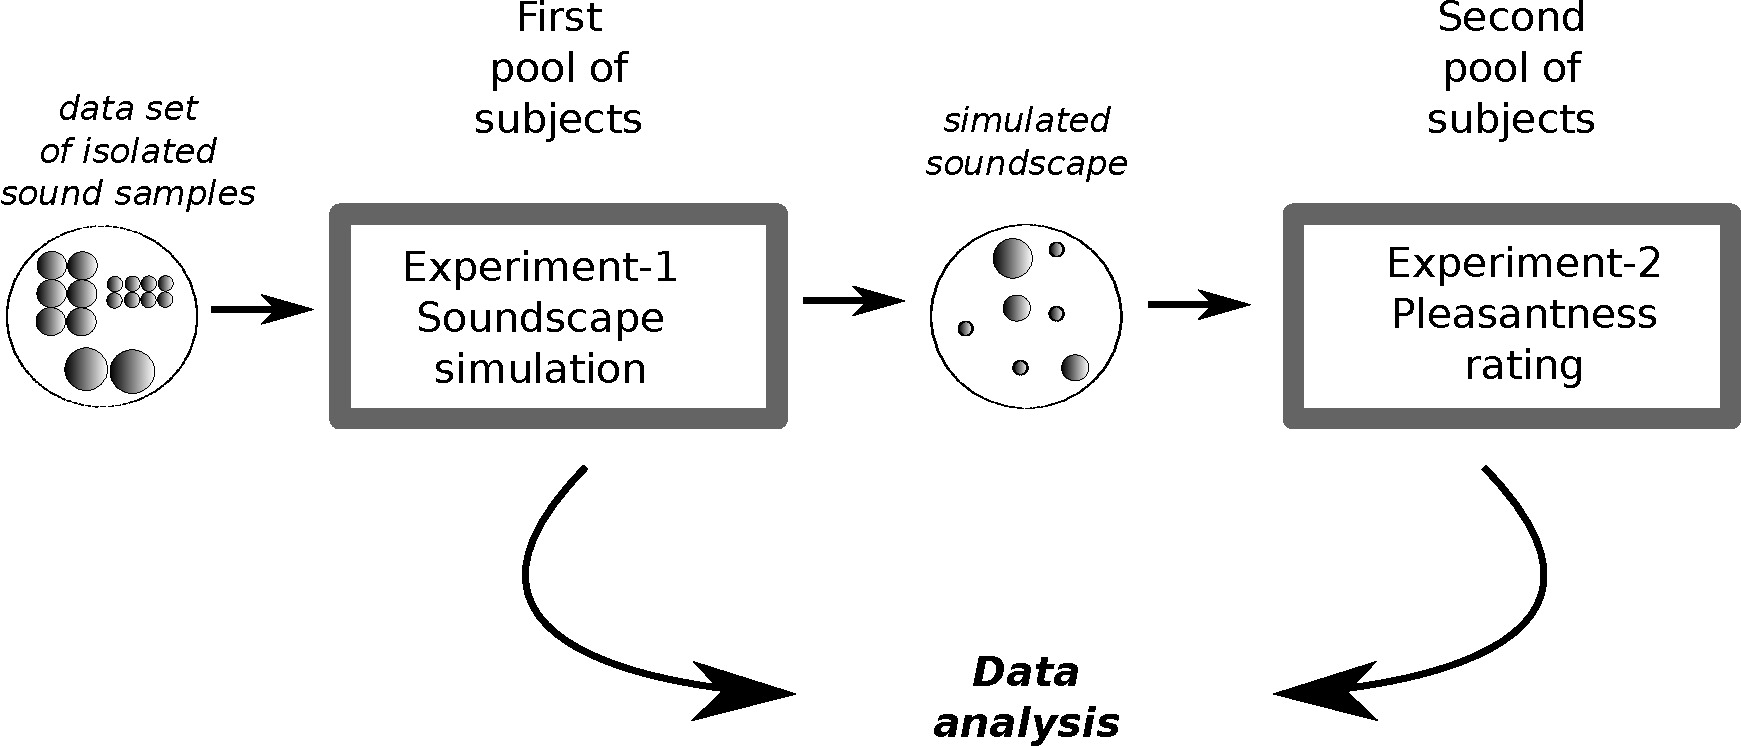
\includegraphics[width=.8\linewidth]{gfx/5}
        \caption{Planification expérimentale des éxperiences de simulation et d'évaluation de l'agrément}\label{fig:xp1_2}
\end{figure}



\subsection{Banque de données de sons isolés}

Dans cette section, nous présentons les processus de sélection et d'acquisition des sons utilisés comme matériau de base lors de la simulation des environnements sonores urbains. La banque de données est identique à celle utilisée dans le cadre de l'expérience pilote \citep{lafay2013atiam,lafay2014new}. 

Pour plus de détails sur l'organisation interne de la banque de données, ainsi que sur l'interface graphique permettant de sélectionner ces dernières, se référer aux sections~\ref{sec:ch4_dbEventTexture} et~\ref{sec:ch4_ssf}.

\subsection{Typologie des sources sonores présentes dans l'environnement urbain}

Afin de créer un corpus de sons isolés de référence pour la simulation, nous avons réalisé une typologie des sons environnementaux urbains. 

Pour ce faire, une étude bibliographique est effectuée, afin d'identifier les sources et ambiances sonores les plus souvent citées dans la littérature. Cette étude porte sur 16 articles ou thèses. Chacun d'eux traite de la manière dont nous discriminons les paysages sonores urbains. Il ressort que plusieurs approches sont possibles :

\begin{itemize}
\item 9 articles abordent le problème par une approche perceptive, soit en identifiant ou répertoriant des catégories de sources sonores, soit en étudiant l'impact de classes de sons spécifiques sur la perception de l'environnement : \cite{maffiolo_caracterisation_1999,raimbault2002simulation,guastavino_etude_2003,defreville2004aactivity,raimbault2005urban,dubois2006cognitive,devergie_relations_2006,guastavino2006ideal,niessen2010categories}
\item 3 articles proposent une classification morpho-typologique, divisant l’environnement sonore urbain en ``\,zones sonores\,'' possédant une identité acoustique forte, selon la configuration et la pratique du site : \cite{maffiolo_caracterisation_1999,beaumont2004pertinence,polack2008perceptive}
\item 2 articles répertorient et classifient les sources sonores d’un point de vue expert : \cite{leobon_analyse_1986,brown2011towards}
\end{itemize}

La nature des classes est établie par rapport aux catégories perceptives, ou classes de sons, les plus souvent citées dans ces publications. À partir des éléments relevés, nous établissons deux taxonomies : une pour les événements (\cf~Figure~\ref{fig:taxonomie}.a), une autre pour les textures (\cf~Figure~\ref{fig:taxonomie}.b). Comme évoqué à la section~\ref{sec:db_ui}, la structure taxonomique de ces deux ensembles s'inspire grandement de l'axe vertical de l'organisation catégorielle proposée par E. Rosch (\cf~Section~\ref{sec:ch3_categoEtAbstract}), \ie~plus le niveau d'abstraction de la classe est élevé, plus la description de la classe est précise, et plus les sources sonores incluses dans cette classe sont semblables (\cf~Figure~\ref{fig:orgDb}). Pour les événements, nous considérons quatre niveaux d'abstraction allant des classes les plus globalisantes (niveau d'abstraction 0), aux classes les plus spécifiques (niveau d'abstraction 3). Pour les textures, nous ne considérons que trois niveaux d'abstraction.

Pour les événements, les regroupements se font en grande majorité par rapport à la source, et sont d’ordre sémantique. Pour les textures, nous considérons également la nature des lieux hébergeant ces dernières (\eg~\emph{parc}, \emph{rue}). La typologie des classes d'événements suit la nomenclature source-action introduite à la section (\cf~Section~\ref{sec:ch4_sourceAction}). En ce sens, elle est très similaire à cette autre typologie de sources sonores urbaines, effectuée postérieurement \citep{Salamon14}.

\begin{figure}[t]
        \myfloatalign
        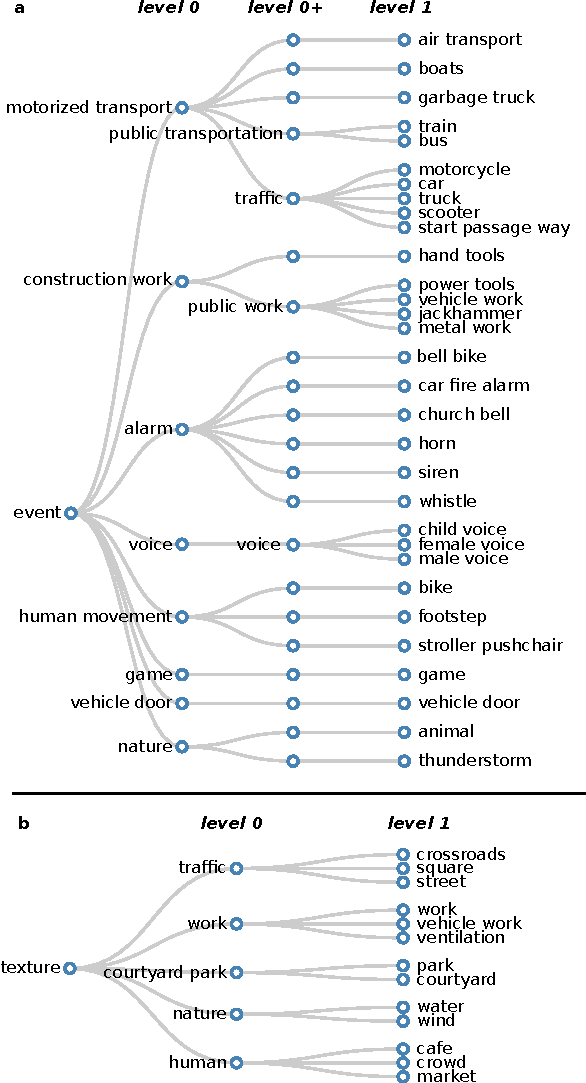
\includegraphics[width=.5\linewidth]{gfxHierarchy/taxonomy}
       \caption[Taxonomies des classes de sons utilisées pour la simulation des environnements sonores urbains]{Taxonomies des classes de sons utilisées pour la simulation des environnements sonores urbains pour (a) les événements sonores, et (b) les textures sonores. Nous présentons ici uniquement les niveaux d'abstraction 0 et 1. Un niveau intermédiare, nommé $0+$, et utilisé pour l'analyse, est également introduit.}\label{fig:taxonomie}
\end{figure}

\subsection{Acquisition des sons isolés}
\label{sec:ch5_recordDataSet}

Sur la base des typologies précédemment établies, 483 sons ont été collectés, dont 381 événements, et 102 textures.

Parmi les événements :

\begin{itemize}
\item 260 sont issus d’enregistrements effectués pour l'étude;
\item 89 sont issus de la banque de sons \emph{SoundIdeas}\footnote{Pour plus de détails sur \emph{SoundIdeas} voir :\url{ http://www.sound-ideas.com/}};
\item 32 sont issus de la banque de sons \emph{Universal SoundBank}\footnote{Pour plus de détails sur \emph{Universal SoundBank} voir : \url{http://www.universal-soundbank.com/}}.
\end{itemize}

Parmi les textures:

\begin{itemize}
\item 72 sont issues d’enregistrements effectués pour l'étude;
\item 23 sont issues de la banque de sons \emph{SoundIdeas};
\item 7 sont issues de la banque de sons \emph{Universal SoundBank}.
\end{itemize}

Tous les enregistrements ont été effectués à l’aide d'un micro canon \emph{AT8035}\footnote{\cf~\url{http://eu.audio-technica.com/fr/products/product.asp?catID=1&subID=6&prodID=1845}} relié à un enregistreur \emph{ZOOM H4n}\footnote{\cf~\url{http://www.zoom.co.jp/english/products/h4n/}}. L’utilisation du micro canon nous permet d’isoler les événements sonores du brouhaha urbain. Pour les textures, il nous permet d’éviter les événements sonores proches du preneur de son. Nous pouvons ainsi pointer des "zones sonores", en nous tenant à une certaine distance de ces dernières, afin de capter uniquement le brouhaha émanant de la zone ciblée.

Tous les sons ont été normalisés au même niveau $RMS$ \footnote{Le niveau $RMS$, de l'anglais \emph{Root Mean Square} qui désigne la valeur efficace d'un signal. Formellement, le niveau $RMS$ $x_{RMS}$ d'un signal $x=(x_1,x_2,\ldots,x_n)$ s'obtient en calculant la moyenne quadratique de ce dernier $x_{RMS}=\sqrt{\dfrac{1}{n}\sum\limits_{i} x_i^2}$} de $-12$ $dB$ (FS) \footnote{$dB$ (FS) est le sigle anglais désignant une valeur en décibels relative à la pleine échelle (\emph{relative to Full Scale}), \ie~le rapport entre le niveau du signal et sa valeur maximale. Dans notre cas, ce niveau pleine échelle est de 1 Volt.}.

\subsection{Planification expérimentale}

\subsubsection{Épreuve de simulation}
\label{sec:ch5_planExpSimu}

Nous nommons cette expérience: \emph{expérience 1.a}. \\

\textbf{Procédure} \\

Les sujets doivent simuler deux environnements sonores urbains, chacune des scènes devant durer 1 minute. Pour ces simulations, les sujets doivent se conformer aux consignes suivantes:

\begin{itemize}
\item première simulation : simuler un paysage sonore \textbf{urbain plausible} qui, selon vous, est idéal (où vous aimeriez vivre);
\item deuxième simulation : simuler un paysage sonore \textbf{urbain plausible} qui, selon vous, est non-idéal (où vous n'aimeriez pas vivre).
\end{itemize}

Tous les sujets commencent par simuler l'environnement idéal. Les sujets ne prennent connaissance de la deuxième consigne qu'à la fin de la première simulation.

Les sujets son totalement libres dans le choix des sons, et des paramètres (pour plus de détails sur les paramètres se référer à la section~\ref{sec:ch4_param}). Ils doivent cependant se soumettre à deux contraintes:

\begin{itemize}
\item le sujet doit prendre le point de vue d’un auditeur fixe;

\item le paysage sonore doit être réaliste, au sens de physiquement plausible. Autrement dit, le sujet à tout à fait le droit de placer 10 chiens dans son paysage sonore, mais il n’a pas le droit de placer un chien aboyant toutes les 10 millisecondes.

\end{itemize}

Ces contraintes font partie de la consigne. Aucun contrôle n'est fait \emph{a priori} dans l'interface de simulation.

Chaque processus de simulation comprend deux parties :

\begin{enumerate}
\item la réalisation de la simulation: cette étape peut, elle même, se décomposer en trois actions (\cf~Section~\ref{sec:ch4_processSimu}):
\begin{itemize}
\item sélectionner les classes de sons
\item nommer les classes de sons sélectionnées
\item paramétrer les pistes (\cf~Section~\ref{sec:ch4_seqSample}) relatives aux classes de sons sélectionnées
\end{itemize}
\item la réalisation d'un commentaire libre du paysage sonore simulé
\end{enumerate}

En complément, et une fois les deux scènes sonores réalisées, les sujets sont invités à:

\begin{itemize}
\item indiquer les sources sonores qu'ils voulaient mettre, mais qu'ils n'ont pas trouvées;
\item commenter l’ergonomie du logiciel de simulation;
\item commenter l’ergonomie de l'interface de sélection.
\end{itemize}

Avant de commencer la première simulation, un tutoriel de 20 minutes est proposé aux sujets, afin qu'ils se familiarisent avec le logiciel de simulation, et la banque de données. Le tableau~\ref{tab:indSimu} résume les étapes de l’expérience, ainsi que leurs durées respectives. L'expérience est prévue pour durer 2h30. \\

\begin{table}[t]
\centering
\begin{tabular}{c c c} 
Index          & Tâche                               & Durée (min) \\                      
\hline
1 & Présentation de l'expérience                     & 10 \\
  & Lecture de la consigne                           &  \\
\hline
2 & Tutoriel (Réalisation d'une scène test)          & 20 \\
\hline
3 & Première simulation: scène idéale                & 40 \\
\hline
4  & Commentaire de la scène idéale                  & 15 \\
\hline
3 & Deuxième simulation: scène non-idéale            & 40  \\
\hline
4  & Commentaire de la scène non-idéale              & 15 \\
\hline
5 & Critique de l'interface de simulation            & 10 \\
  & et de l'interface de sélection                   & \\
\hline
\end{tabular}
\vspace{0.5mm}
\caption{Résumé des étapes de l’expérience de simulation}
\label{tab:indSimu}
\end{table}

\textbf{Apparatus} \\

Tous les sujets passent l'expérience sur des machines identiques (\gl{description des machines}). L'audio est diffusé en stéréophonie, par le biais de casques audio. Pendant le tutoriel, les sujets doivent ajuster le niveau sonore à un volume confortable. Ils ne peuvent le modifier par la suite.

Tous les sujets réalisent l'expérience simultanément. Ils sont répartis de manière égale dans trois pièces identiques, toutes possédant un environnement calme. Ils n'ont pas le droit de s'adresser la parole pendant l'expérience.

Trois expérimentateurs, un dans chaque pièce, sont présents durant la totalité de l'expérience, afin de contrôler le bon déroulement de cette dernière, et de répondre aux éventuelles questions des sujets.  \\

\textbf{Participants} \\

44 étudiants (14 femmes) de L’École Centrale de Nantes ont participé à l'expérience. Ils ont tous sensiblement le même âge (moyenne: 21.6, écart-type: 2). Tous les sujets sont Nantais, et vivent dans cette ville depuis deux ans ou plus.

Sur les 44 sujets, 40 réalisent l'expérience avec succès, produisant au final 80 scènes sonores simulées, dont 40 scènes idéales, et 40 scènes non idéales. 4 sont éliminés pour non respect et/ou incompréhension des consignes, d'une part, dépassement du temps, d'autre part.



\subsubsection{Épreuve d'évaluation de l'agrément}
\label{sec:ch5_planExpEvaA}

Nous nommons cette expérience: \emph{expérience 1.b}. \\

\textbf{Procédure} \\

En raison de contraintes temporelles, les sujets n'évaluent que des séquences de 30 secondes des scènes simulées, chacune de ces séquences commençant à la seconde 15, et finissant à le seconde 45, de la scène évaluée.

L'évaluation s'effectue sur une échelle sémantique bipolaire de 7 points, allant de -3 (non-idéale/très désagréable) à +3 (idéale/très agréable). Avant de noter une scène, les sujets doivent obligatoirement écouter les 20 premières secondes de cette dernière. Après la notation, ils sont libres de passer à la scène suivante.

Pour chaque sujet, les scènes sont présentées dans un ordre aléatoire. Les 10 premières scènes permettent au sujet de calibrer ses notes. Elles sont obligatoirement composées de 5 scènes idéales et de 5 non-idéales. Ces 10 premières scènes sont rejouées à la fin de l'expérience, et seules les notes données à la deuxième occurrence sont prises en compte. 

L'expérience est prévue pour durer 30 minutes. Les sujets ne connaissent pas la nature des scènes.\\

\textbf{Apparatus} \\

Tous les sujets passent l'expérience sur des machines identiques (\gl{description des machines}). L'audio est diffusé en stéréophonie, par le biais de casques audio semi-ouvert \emph{Beyer-Dynamic DT 990 Pro}. Toutes les scènes sonores ont été re-simulées sur la base des partitions obtenues lors de l'expérience de simulation. Le niveau sonore de sortie est identique pour tous les sujets.

Tous les sujets réalisent l'expérience simultanément, dans un environnement calme. Ils n'ont pas le droit de s'adresser la parole pendant l'expérience. 

Un expérimentateur est présent durant la totalité de l'expérience, afin de contrôler le bon déroulement de cette dernière, et de répondre aux éventuelles questions des sujets.  \\

\textbf{Participants} \\

10 étudiants (2 femmes) de L’École Centrale de Nantes ont participé à l'expérience. Aucun d'entre eux n'a réalisé l'expérience de simulation. Tous les sujets ont sensiblement le même âge (moyenne: 23.1, écart-type: 1.8). Tous les sujets sont Nantais, et vivent dans cette ville depuis deux ans ou plus.

Tous les sujets ont réalisé l'expérience avec succès.

\subsection{Données et méthodes d'analyses}

\subsubsection{Nature des données analysées}
\label{sec:ch5_dataType1}

A partir des données produites par l'épreuve de simulation, nous analysons:

\begin{itemize}
\item les partitions des scènes simulées;
\item les signaux des scènes simulées;
\item les commentaires sur les sons manquants, et l'ergonomie des interfaces de simulation et de sélection.
\end{itemize}

Chaque scène est décrite par un groupe de descripteurs. C'est sur la base de ces descripteurs que nous pratiquons l'analyse. Un résumé des descripteurs, ainsi que des acronymes les désignant, est présenté dans le Tableau~\ref{tab:acronyme}. Afin de rester cohérent avec l'épreuve d'évaluation, les descripteurs issus des partitions, ou des signaux des scènes, ne sont pas calculés sur la durée totale de celles-ci, mais sur une version réduite de 30 secondes (\cf~Section~\ref{sec:ch5_planExpEvaA}). 

Pour chaque scène sonore, trois types de descripteurs sont considérés:

\begin{itemize}
\item \emph{perceptif}: il s'agit de l'agrément perçu de la scène simulée, évalué sur une échelle sémantique 7 points. Nous notons $\mathcal{A}_{scene}$ l'agrément moyen d'une scène, obtenu en moyennant les notes de tous les sujets. De même, nous notons  $\mathcal{A}_{sujet}$ l'agrément par sujet, en moyennant l'ensemble de ses notes. Compte tenu du faible nombre de sujets, nous faisons le choix, dans cette étude, de ne pas normaliser les notes d'agrément;
\item \emph{sémantique}: il s'agit d'un vecteur booléen noté $S=(x_1,x_2,\ldots,x_n)$, indiquant les classes de sons présentes dans la scène. Chaque point $x$ de ce vecteur correspond à une classe de sons particulière: $x=1$ si la classe est présente dans la scène, et $x=0$ autrement. La dimension $n$ des vecteurs dépend du niveau d'abstraction considéré, \eg~pour le niveau d'abstraction 1, qui comprend $44$ classes de sons, cette dimension sera de $n=44$.
\item \emph{structurel}: Les descripteurs structurels sont calculés à partir des partitions et des signaux des scènes simulées. Trois descripteurs structurels sont envisagés:
\begin{itemize}
\item \emph{diversité} ($DIV$) : il s'agit d'un scalaire représentant la diversité des classes sonores utilisées pour simuler une scène. Nous calculons $DIV$ en comptant le nombre de classes de sons distinctes utilisées pour une simulation. Ce nombre dépend du niveau d'abstraction considéré. Par exemple, considérant les deux sous classes du niveau d'abstraction 2 \emph{passage de voiture} et \emph{démarrage de voiture}, toutes deux appartenant à la classe \emph{voiture} du niveau d'abstraction 1, nous comptons deux classes pour la diversité des niveaux d'abstraction 2, et 1, et seulement 1, pour les niveaux d'abstraction 0 et 1;
\item \emph{densité} ($D$) : il s'agit d'un scalaire représentant le nombre de sources sonores présentes en moyenne. Pour obtenir $D$, nous calculons le logarithme du nombre d'éléments sonores par fenêtre de 125 millisecondes (sans recouvrement), et moyennons au cours du temps. Le calcul de $D$ peut inclure toutes les sources sonores de la scène, ou seulement une partie. Dans ce cas, les fenêtres ne contenant pas de sources sonores ne sont pas prises en compte. Nous notons $D(E)$ et $D(T)$ les densités calculées en considérant séparément les sources d'événements et de textures sonores;
\item \emph{niveau Sonore} ($L$) : pour représenter le niveau sonore, nous nous inspirons de la mesure $L_{Aeq}$. Dans notre cas, il s'agit d'un scalaire, calculé sur le signal en volts, et non en pression, et donné en décibels, en prenant un référentiel de 1 Volt. Le niveau est obtenu en calculant, toutes les secondes, la moyenne quadratique du signal, et en moyennant sur la durée de la scène. Un filtrage de type A est opéré avant le calcul des moyennes quadratiques. D'autre descripteurs, inspirés eux aussi de descripteurs acoustiques classiques ($L_{Amin}$, $L_{Amax}$, $L_{A10-90}$), et utilisant un opérateur autre que la moyenne (minimum, maximum, les 10-90ème quantiles) pour intégrer les fenêtres de 1 seconde, ont été testés. Mais, ces derniers présentant tous une corrélation élevée avec $L$ ($r_{pearson}\geq0.76$, $p<0.01$), nous conservons le scalaire ci-devant mentionné comme unique descripteur objectif du niveau sonore.
\end{itemize}
\end{itemize}

\begin{table}[t]
\centering
\begin{tabular}{c c c c c} 
Descripteurs          & Acronymes   &   & Descripteurs            & Acronymes  \\                       
\cline{1-2} \cline{4-5}
Densité               & $D$         &   & Diversité               & $DIV$    \\
                      &             &   &                         &          \\
Densité               & $D(E)$      &   & Diversité               & $DIV(E)$ \\
(événements)          &             &   & (événements)            &          \\
Niveau                & $L$         &   & Diversité               & $DIV(T)$ \\
                      &             &   & (textures)              &          \\
Niveau                & $L(E)$      &   & Agrément moyen          & $\mathcal{A}_{scene}$     \\
(événements)          &             &   & (par scène)             &         \\
Niveau                & $L(T)$      &   & Agrément moyen          & $\mathcal{A}_{sujet}$        \\
(textures)            &             &   & (par sujet)             &      \\
                      &             &   &                         &      \\
\multicolumn{3}{c}{Termes} &  \multicolumn{2}{c}{Acronymes} \\ 
\hline
\multicolumn{3}{c}{Idéal/agréable}                 & \multicolumn{2}{c}{i}       \\
\multicolumn{3}{c}{non-idéale/désagréable}         & \multicolumn{2}{c}{ni}      \\
\multicolumn{3}{c}{Scène idéale/agréable}          & \multicolumn{2}{c}{i-scène} \\
\multicolumn{3}{c}{Scène non-idéale/désagréable}   & \multicolumn{2}{c}{ni-scène} \\
\hline
\end{tabular}
\vspace{0.5mm}
\caption{TODO}
\label{tab:acronyme}
\end{table}

\subsubsection{Méthodologie et Outils statistiques}
\label{sec:ch5_methodoEtStat1}

Afin d'évaluer l'impact spécifique des différentes sources sonores sur l'agrément perçu, nous soumettons nos travaux aux 6 tests/études de significativité présentés ci-après:

\begin{itemize}
\item \emph{étude qualitative} : afin de vérifier la validité écologique de 1) la banque de données et 2) l'interface de sélection, nous réalisons une étude qualitative des critiques ergonomiques effectuées par les sujets;
\item \emph{étude comparative entre les descripteurs structurels} : afin d'évaluer si la distinction affective imposée entre les i- et ni-scènes impacte de manière significative la nature des scènes, \ie~s'il existe des différences significatives entre les descripteurs structurels et/ou l'agrément perçu, nous évaluons cette significativité à partir d'un test de Student à deux échantillons appariés (\cf~Annexe~\ref{app:student});
\item \emph{étude de l'influence des descripteurs structurels sur l'agrément perçu}: afin d'évaluer l'impact potentiel des descripteurs structurels sur l'agrément perçu, nous étudions l'existence de corrélations linéaires entre ces deux types de descripteurs. Pour mesurer la corrélation, nous utilisons le coefficient de Pearson (\cf~Annexe~\ref{app:corr}). Nous adoptons ici une méthodologie couramment utilisée dans l'approche dimensionnelle;
\item \emph{étude comparative entre les descripteurs sémantiques}: afin d'apprécier si la distinction affective imposée a eu un impact sur la composition des scènes en terme de sources sonores, ou, pour être plus précis, s'il existe des classes de sons qui ont été particulièrement utilisées pour simuler un type d'environnement, nous utilisons le V-test. Nous vérifions si la présence d'une classe de sons est typique d'un environnement (i ou ni). Le test est effectué pour chaque niveau d'abstraction, et séparément, pour les classes d'événements et de textures. Pour chaque classe $j$ et chaque type d'environnements $k$ ($k={i,ni}$), la valeur $V_{jk}$ du V-test se calcule comme suit: 

\begin{equation*}
V_{jk}=\dfrac{c_{jk}-c_k\frac{c_j}{c}}{\sqrt{c_k\frac{c-c_k}{c-1}\frac{c_j}{c}(1-\frac{c_j}{c})}}
\end{equation*}

où $c$ est le nombre de classes utilisées, $c_k$ le nombre de classes utilisées pour un type d'environnements $k$, $c_j$ le nombre de classes $j$ utilisées, et $c_{jk}$ le nombre de classes $j$ utilisées pour un type d'environnements $k$. Le V-test teste l'hypothèse nulle que la proportion $\frac{c_{jk}}{c}$ ne diffère pas significativement de la proportion $\frac{c_{jk}}{c_k}$. Si pour un environnement $k$, et une classe $j$, l'hypothèse est rejetée, la classe $j$ est alors typique de l'environnement $k$. Les classes typiques sont nommées \textbf{marqueurs sonores};

\item \emph{étude des espaces de représentations induits par les descripteurs sémantiques}: afin d'étudier si une représentation basée uniquement sur la présence ou l'absence des classes de sons permet de séparer les deux types d'environnements, nous considérons l'espace induit par les descripteurs sémantiques $S$. $S$ étant un vecteur booléen, nous calculons les distances entre les scènes à partir de la distance de Hamming. Considérant les deux vecteurs $S_1=(x_{1,1},x_{1,2},\ldots,x_{1,n})$, et $S_2=(x_{2,1},x_{2,2},\ldots,x_{2,n})$ de dimension $n$, avec $x={0,1}$, la distance de Hamming $d_{ham}$ mesure le pourcentage de coordonnées qui diffèrent entre les deux vecteurs:   


\begin{equation*}
d_{ham}(S_1,S_2)=\dfrac{1}{n}\sum_{i=1}^{n} (x_{1,i} \bigoplus x_{2,i})
\end{equation*}

où $\bigoplus$ désigne l'opérateur du \emph{ou-exclusif}. plus la composition des deux scènes est similaire, et plus ces deux scènes sont proches. L'utilisation de la distance de Hamming permet de prendre en compte de manière égale les classes présentes et absentes. Pour mesurer la capacité intrinsèque de l'espace à séparer les i- et ni-scènes, nous utilisons une métrique de \emph{clustering} nommée précision au rang $k$ ($P@k$). La $P@k$ mesure la précision obtenue après que $k$ items ont été retrouvés. Formellement, pour chaque scène $s_i$, nous calculons le rapport entre le nombre de scènes $s_j$, prises parmi les $k$ plus proches voisines de $s_i$, et  partageant le même label que $s_i$, sur le nombre d'items à retrouver ($k$). La $P@k$ est alors la moyenne des rapports pour tous les items;

\item \emph{étude de l'influence spécifique des marqueurs sonores sur l'agrément perçu}: afin d'évaluer les contributions spécifiques de certaines sources sonores, nous évaluons une nouvelle fois l'impact potentiel des descripteurs structurels sur l'agrément perçu, mais en ne tenant compte, cette fois, que des marqueurs sonores pour calculer ces descripteurs.
\end{itemize}

Excepté le V-test, tous les tests de significativité sont effectués avec un seuil critique $\alpha=0.05$. Pour le V-test, étant donné que nous testons beaucoup de classes, une correction de Bonferroni (\cf~Annexe~\ref{app:statuni}) est appliquée. Pour les valeurs $p$, dans le cas où la valeur $p\geq0.05$, nous indiquons sa valeur. Dans le cas ou $0.01\leq p<0.05$, nous indiquons seulement $p<0.05$. Dans le dernier cas nous indiquons $p<0.01$.

Concernant l'interprétation du coefficient de corrélation de Pearson adoptée dans ce document, nous invitons le lecteur à se référer à l'annexe~\ref{app:corr}.

\subsection{Validité écologique de l'expérience}

\subsubsection{Diversité de la banque de sons}

Nous voulons vérifier que la diversité des classes de sons proposées est suffisante pour pouvoir simuler un environnent sonore. Nous analysons les commentaires des sujets sur la banque de données. 63\% d'entre eux indiquent avoir été, au moins une fois, dans l'incapacité de trouver un son, avec un maximum de 4 sons par sujet. Parmi les sons manquants relevés, nous identifions 26 classes de sons dont:

\begin{itemize}
\item 16 sont bien présentes dans la banque de données, l'incapacité des sujets à les trouver n'étant donc pas imputable à la diversité de la base.
\item 1 fait référence à des sons de musique, que nous avons choisi délibérément d'occulter. \gl{TODO discuter avant}
\item 9 sont effectivement absentes.  
\end{itemize}

Concernant ces dernières, nous observons qu'il s'agit de classes très spécifiques (\eg~\emph{voiture de sport} ou \emph{voix d'adolescent}), et qui peuvent être remplacées par des classes similaires (\eg~\emph{voiture}, \emph{voix d'enfant} ou \emph{voix d'adulte}). Nous en concluons que la diversité proposée par la banque de sons est satisfaisante et suffisante dans le cadre de notre étude.

\subsubsection{Ergonomie de l'interface de sélection}

Nous voulons vérifier l'efficience de l'interface de sélection. Nous analysons les retours des sujets. $32.5\%$ d'entre eux indiquent spontanément que l'interface est un moyen ``\,simple et efficace\,'' de sélectionner des sons sans l'aide de texte. $57.5\%$ ne font pas mention de difficultés particulières, $10\%$ signalent enfin avoir rencontré des difficultés avec l'interface, sans toutefois que la simulation en ait été affectée.

Nous en concluons que l'interface de sélection, sans texte, ne perturbe pas les sujets outre mesure. Un même constat avait été tiré de l'expérience pilote \citep{lafay2013atiam,lafay2014new}. \\

\gl{TODO: vérifier une dernière fois}

\subsubsection{Ergonomie de l'interface de simulation}

\subsection{Vérification de l'agrément des scènes simulées}

Nous analysons ici l'agrément perçu des $80$ scènes sonores simulées. La Figure~\ref{fig:xp2_Aa} affiche l'agrément moyen $\mathcal{A}_{scene}$ pour les i- et ni-scènes. 

Dans un premier temps, et afin de garantir la cohérence de nos données, nous voulons nous assurer qu'aucune ni-scène n'ait un $\mathcal{A}_{scene}$ supérieur à celui d'une i-scène. Quatre des scènes ne respectent pas la contrainte. Elles et leurs correspondantes i ou ni sont retirées. 36 i-scènes et 36 ni-scènes restent dans le champ de l'analyse.

Dans un deuxième temps, nous voulons tester si les sujets ont bien perçu une différence d'agrément entre les i- et ni-scènes. Pour ce faire, nous observons l'agrément moyen de chaque sujet $\mathcal{A}_{sujet}$, calculé séparément, pour chaque type d'environnement (\cf~Figure~\ref{fig:xp2_Ab}). Il apparaît que les i-scènes ont bien été perçues comme significativement plus agréables ($p<0.01$) que les ni-scènes.

\begin{figure}[t]
        \myfloatalign
        \subfloat[]
        {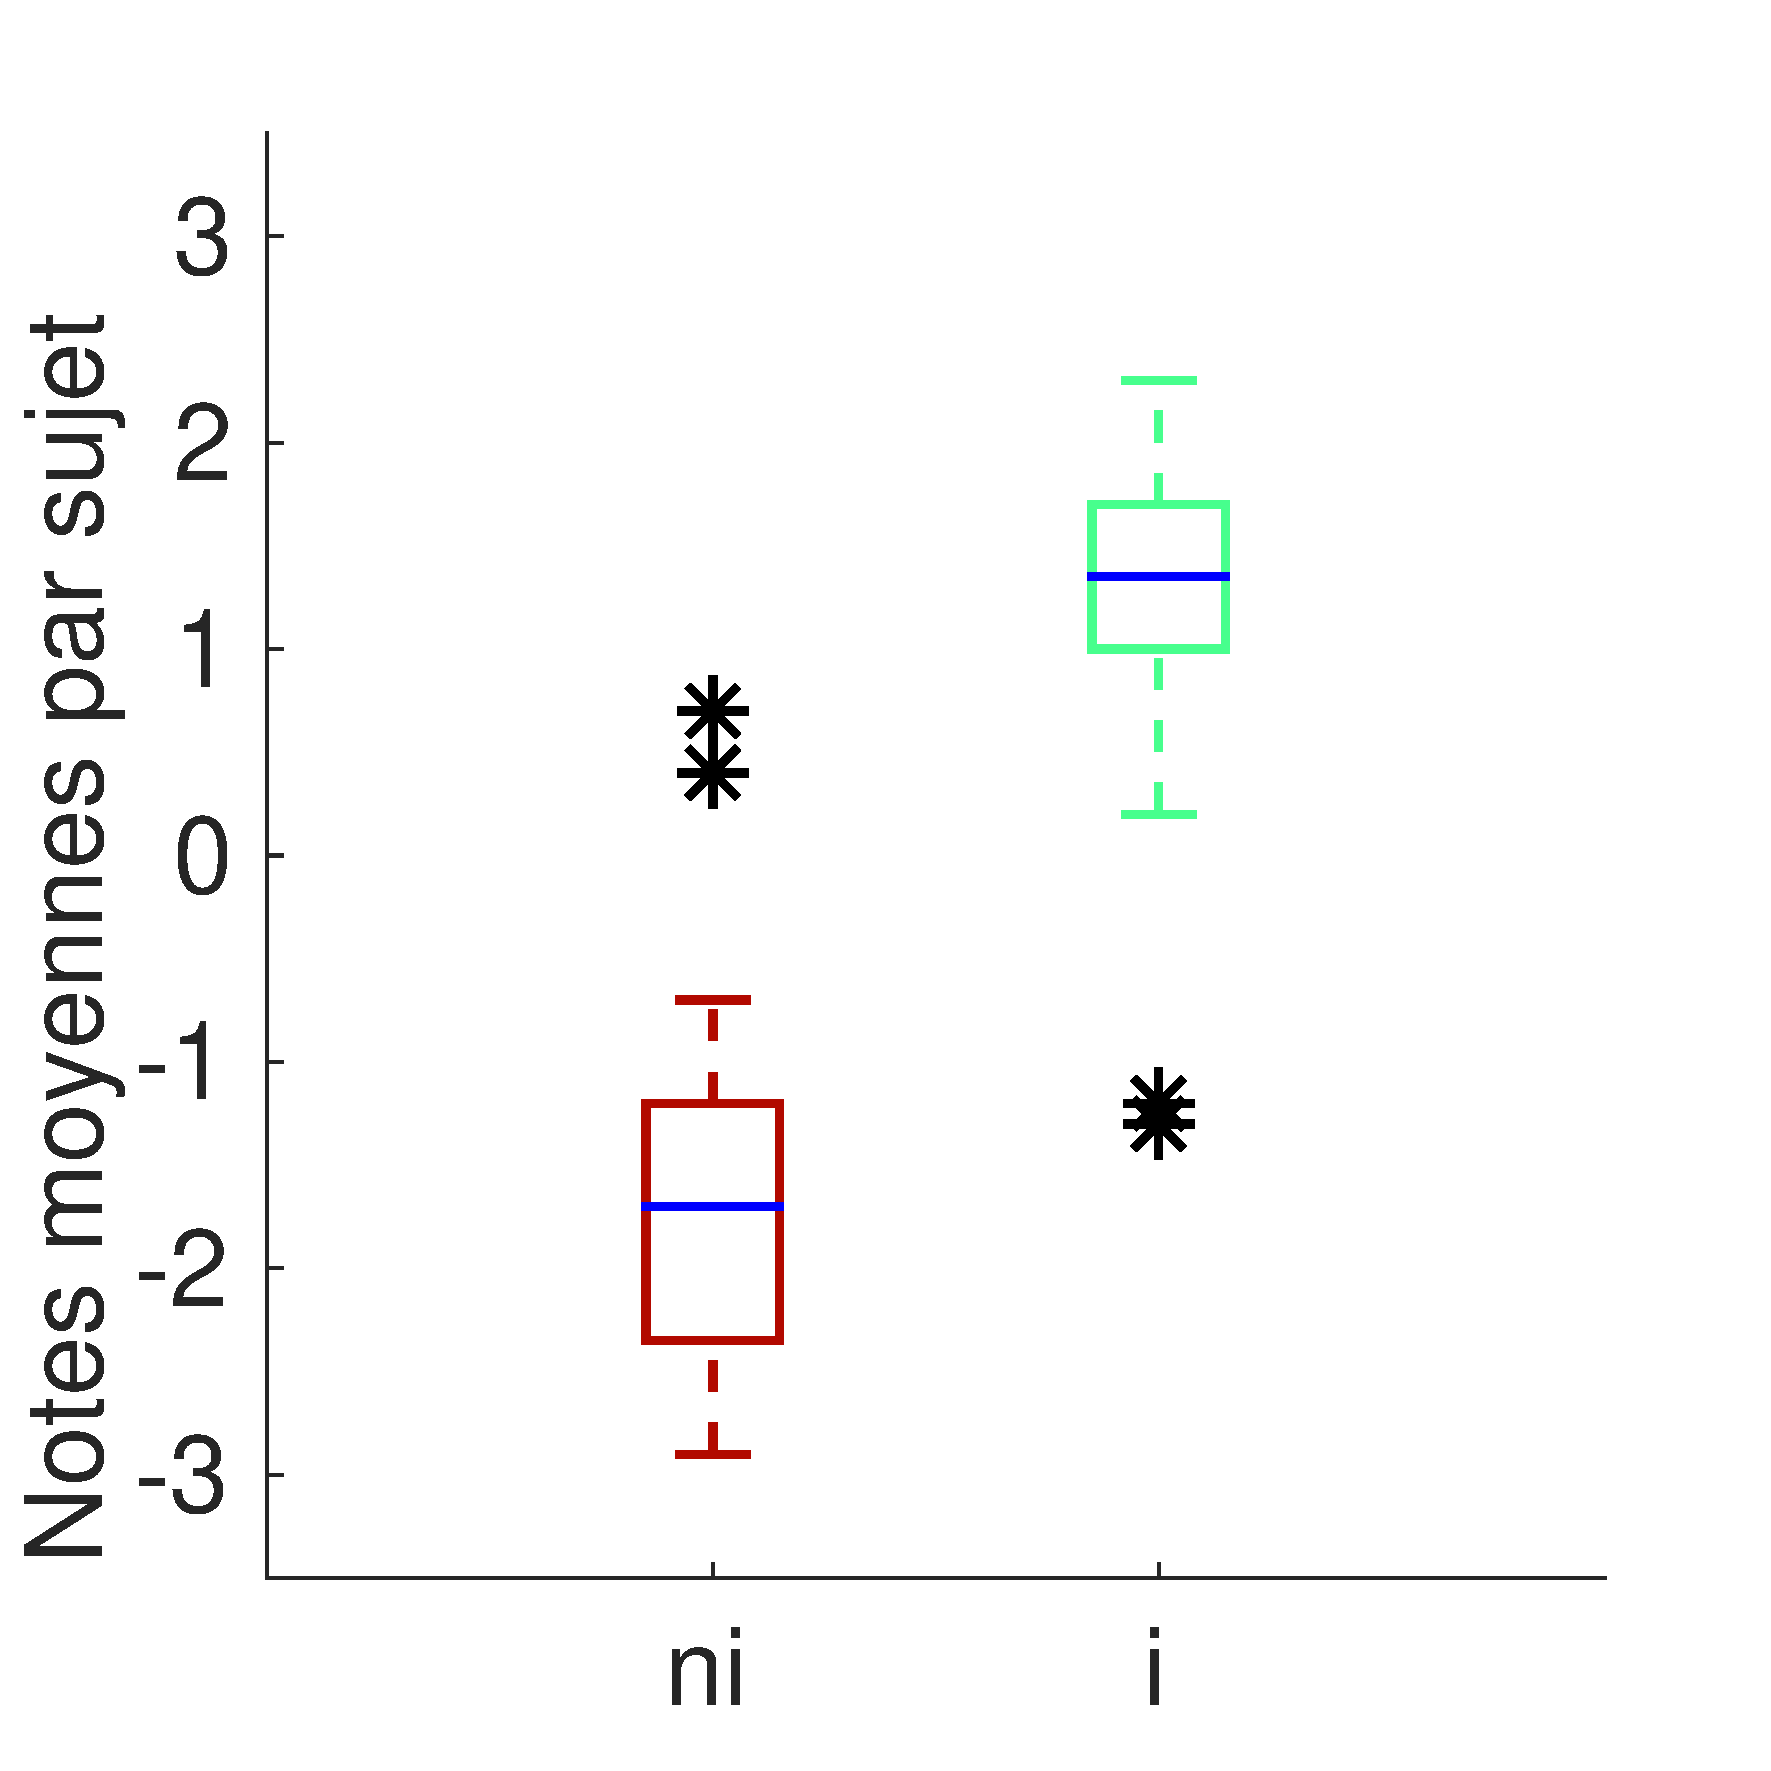
\includegraphics[width=.4\linewidth]{gfxXpUrbanSoundscape/xp2_1}\label{fig:xp2_Aa}}
        \subfloat[]
        {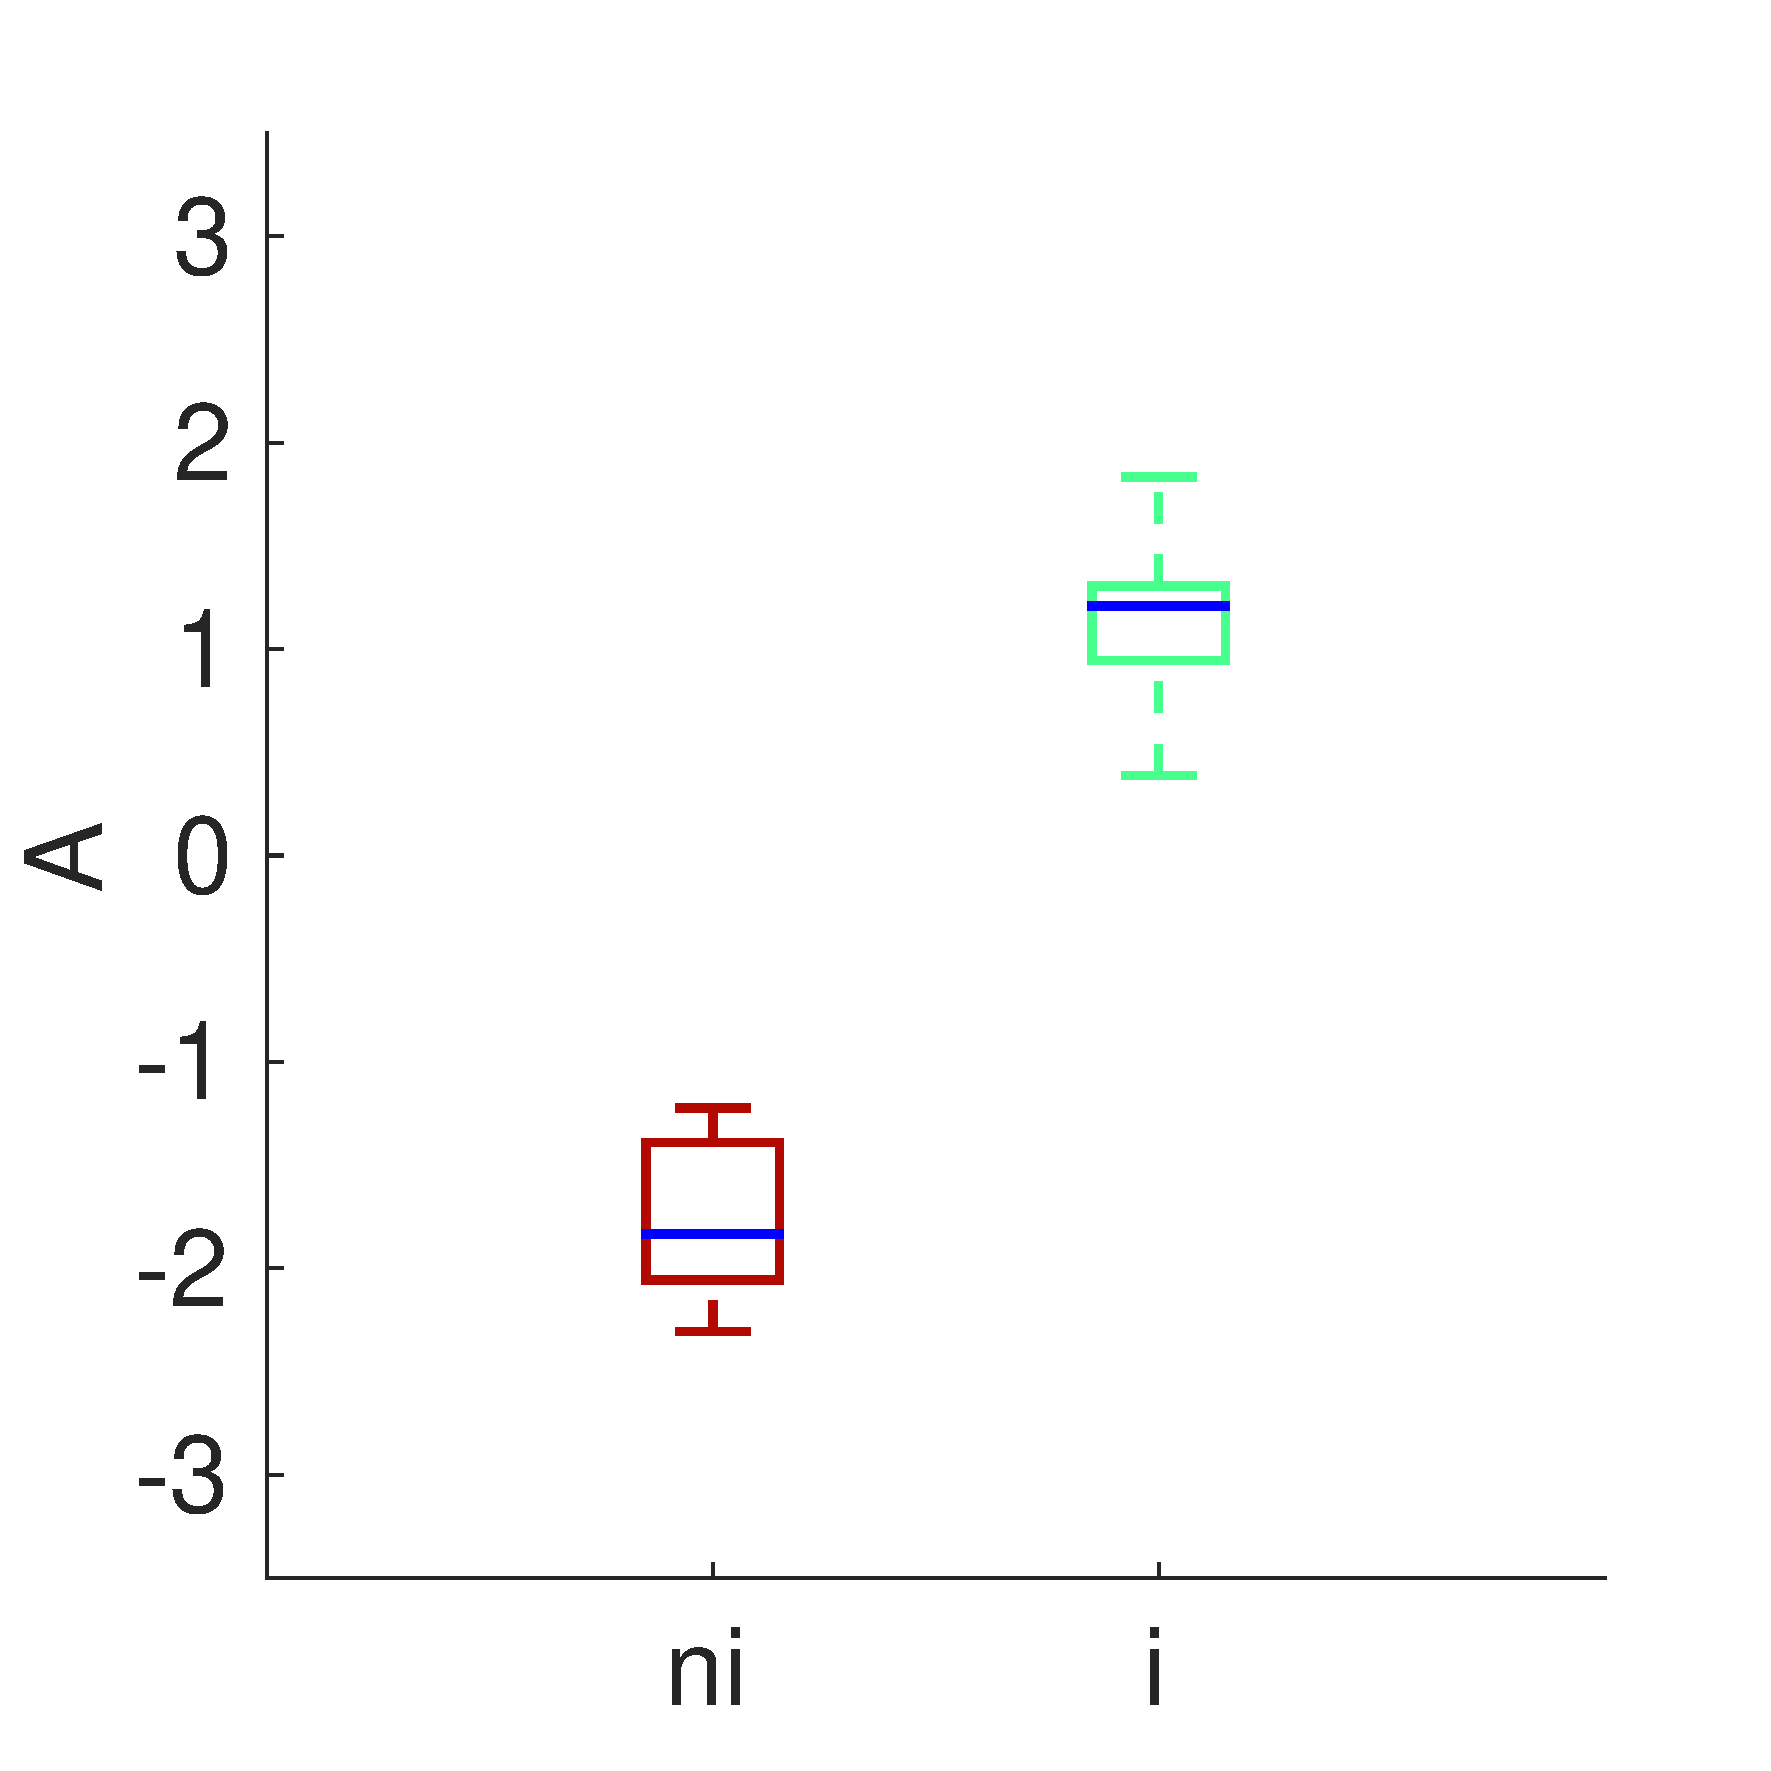
\includegraphics[width=.4\linewidth]{gfxXpUrbanSoundscape/xp2_2}\label{fig:xp2_Ab}}
       \caption[TODO]{TODO}\label{fig:xp2_A}
\end{figure}
 
\subsection{Étude comparative entre les descripteurs structurels}

En premier lieu, nous nous concentrons sur le niveau sonore. Les figures~\ref{fig:soundlevela},~\ref{fig:soundlevelb} et~\ref{fig:soundlevelc} affichent les distributions des niveaux $L$, $L(E)$ et $L(T)$. Il existe bien une différence de niveau  significative entre les i- et ni-scènes ($L$: $p<0.01$), avec un écart moyen de -7 $dB$. Cette différence affecte aussi bien les événements ($L(E)$: $p<0.01$, écart moyen: -7 $dB$) que les textures ($L(T)$: $p<0.01$, écart moyen: -6 $dB$). 

Nous vérifions, sans surprise, que le niveau des sources sonores est bien un indicateur d'agrément, les ni-scènes ayant tendance à être plus fortes, \gl{fait reporté dans un grand nombre d'études} \gl{TODO: citation}. Nous constatons encore que cette différence de niveaux s'observe de manière égale pour les événements et les textures sonores. 

Il apparaît que ce sont les événements qui impactent le plus le niveau global des scènes, l'écart entre $L$ et $L(E)$ n'étant que de 1 $dB$ pour les i-scènes et les ni-scènes. Cette observation fait écho aux résultats obtenus par Kuwano~\al \citep{kuwano_memory_2003}. Au cours de leur expérience, les auteurs demandent à leurs sujets d'évaluer une série d'environnements sonores, d'abord, de manière globale, ensuite, d'en évaluer le niveau aux instants où chacun identifie une source sonore. L'étude montre qu'il n'y a pas de différences significatives entre les jugements globaux et les moyennes des jugements instantanés. Pour en revenir à notre expérience, c'est comme si nos sujets avaient inconsciemment tenu compte de cette réalité perceptive lors de la simulation, en faisant porter le niveau sonore global par des sons courts et bien identifiés, \ie~les événements.

Nous observons, enfin, que le niveau seul ne permet pas de clairement faire la distinction entre les différents types d'environnements. En effet, $20\%$ des i-scènes ont un niveau supérieur au niveau minimal des ni-scènes, alors qu'il n'y a pas de recouvrement, si l'on considère l'agrément perçu $\mathcal{A}_{scene}$.

En second lieu, nous nous penchons sur les densités de sources sonores. Les Figures~\ref{fig:densitya} et~\ref{fig:densityb} affichent les distributions de $D$ et $D(E)$. Que l'on prenne en compte toutes les sources, ou uniquement les événements, la densité est significativement plus élevée pour les ni-scènes ($D$: $p<0.01$, $D(E)$: $p<0.01$). Nous observons un écart moyen de $+0.36$ pour $D$ (soit en moyenne 2.3 sources sonores par fenêtre de plus pour les ni-scènes), et de $+0.32$ pour $D(E)$ (soit en moyenne 2.1 sources sonores par fenêtre de plus pour les ni-scènes). Si ces écarts sont très similaires, c'est que la densité des textures $D(T)$ ne varie pas de manière significative entre les i- et ni-scènes ($D(T)$: $p<0.08$), l'écart moyen étant de $+0.17$ (soit en moyenne 0.7 sources sonores par fenêtre de plus pour les ni-scènes), et l'écart médian étant, quant à lui, nul.

Nous constatons ici que la densité peut être un indicateur de qualité, si l'on considère uniquement les événements sonores. Comme pour les niveaux sonores, la densité ne permet pas de clairement séparer les i- et ni-scènes,  $43\%$ des i-scènes ayant un $D(E)$ supérieur à la densité d'événement minimale des ni-scènes.

En dernier lieu, nous nous intéressons à la diversité. Nous affichons sur la figure~\ref{fig:diversity} $DIV(E)$ et $DiV(T)$, en séparant les différents niveaux d'abstractions. Excepté pour le niveau d'abstraction 0, la diversité de classes d'événements sonores est plus élevée pour les ni-scènes ($DIV(E)$ niveaux 1,2 et 3: $p<0.01$ ), avec en moyenne 2 classes présentes en plus. Aucune différence significative n'est observée pour les textures.

Les tendances globales observées montrent, d'une part, qu'un environnement sonore non-idéal est plus fort, plus dense, et composé d'une plus grande variété d'événements sonores, qu'un environnement sonore idéal. Elles montrent, d'autre part, que ce sont les caractéristiques des événements, plus que celles des textures, qui semblent porter la distinction entre les i- et ni-scènes. Cependant, aucun des descripteurs ne permet, à lui seul, de faire une distinction nette entre les deux types d'environnements, distinction pourtant perçue de manière non ambiguë par les sujets.

\begin{figure}[t]
        \myfloatalign
        \subfloat[]
        {\includegraphics[width=.33\linewidth]{gfxXpUrbanSoundscape/xp_soundlevel_1}\label{fig:soundlevela}}
        \subfloat[]
        {\includegraphics[width=.33\linewidth]{gfxXpUrbanSoundscape/xp_soundlevel_3}\label{fig:soundlevelb}}
        \subfloat[]
        {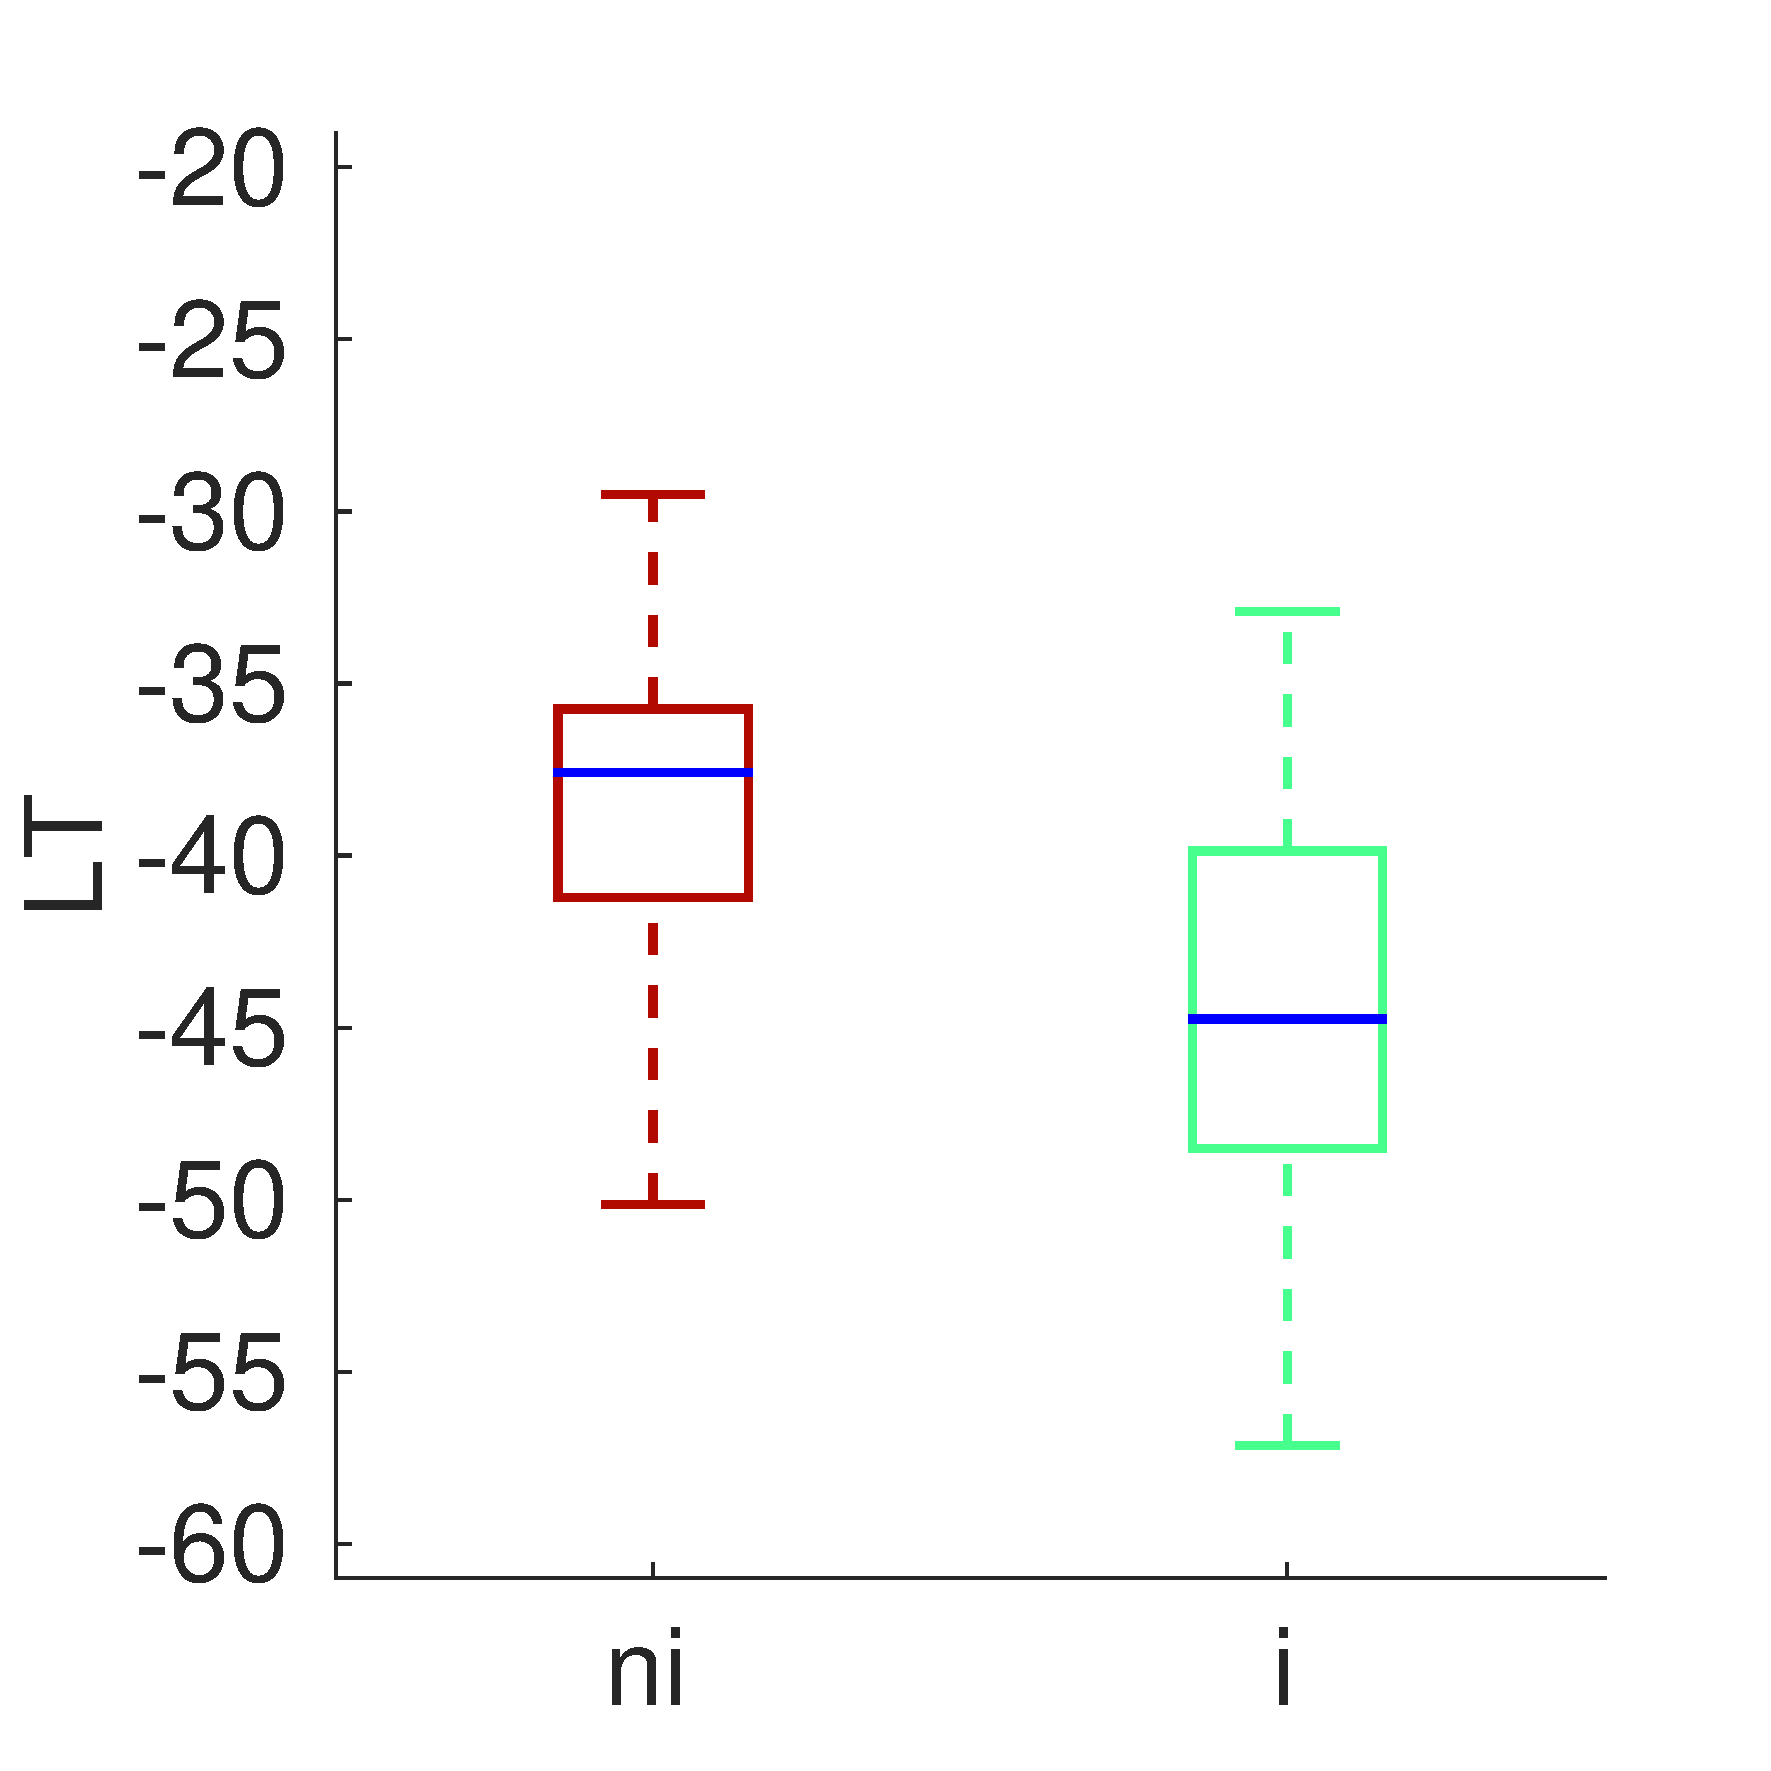
\includegraphics[width=.33\linewidth]{gfxXpUrbanSoundscape/xp_soundlevel_5}\label{fig:soundlevelc}}\par
        \subfloat[]
        {\includegraphics[width=.33\linewidth]{gfxXpUrbanSoundscape/xp_soundlevel_2}\label{fig:soundleveld}}
        \subfloat[]
        {\includegraphics[width=.33\linewidth]{gfxXpUrbanSoundscape/xp_soundlevel_4}\label{fig:soundlevele}}
        \subfloat[]
        {\includegraphics[width=.33\linewidth]{gfxXpUrbanSoundscape/xp_soundlevel_6}\label{fig:soundlevelf}}
       \caption[TODO]{TODO}\label{fig:soundlevel}
\end{figure}

\begin{figure}[t]
        \myfloatalign
        \subfloat[]
        {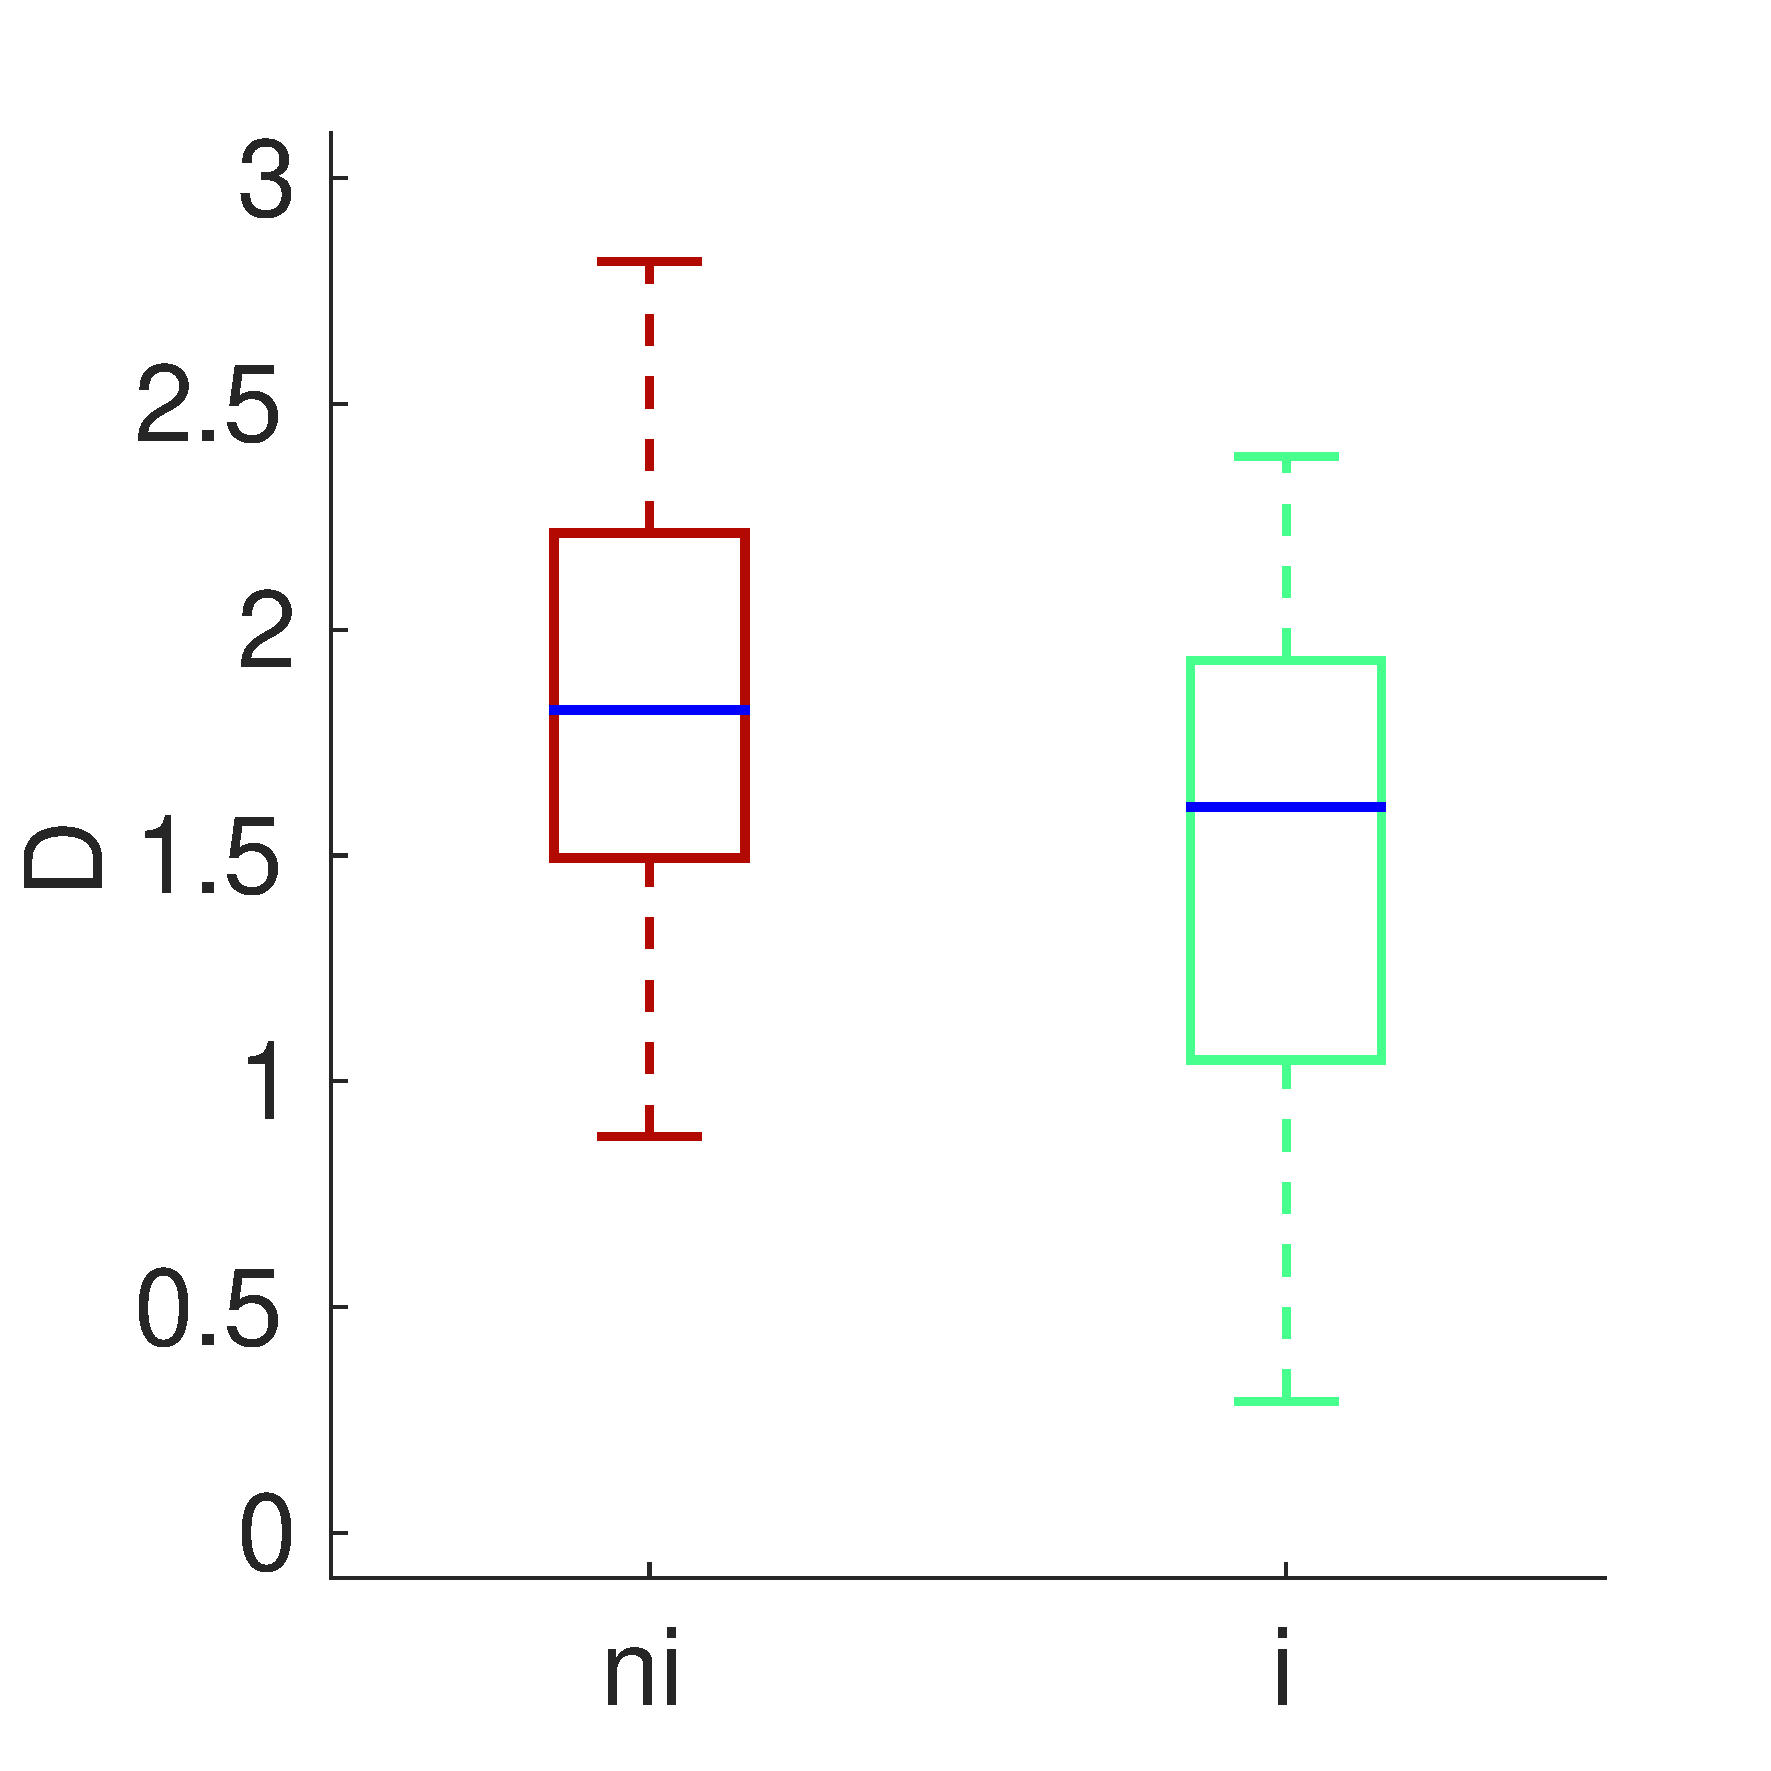
\includegraphics[width=.33\linewidth]{gfxXpUrbanSoundscape/xp_density_1}\label{fig:densitya}}
        \subfloat[]
        {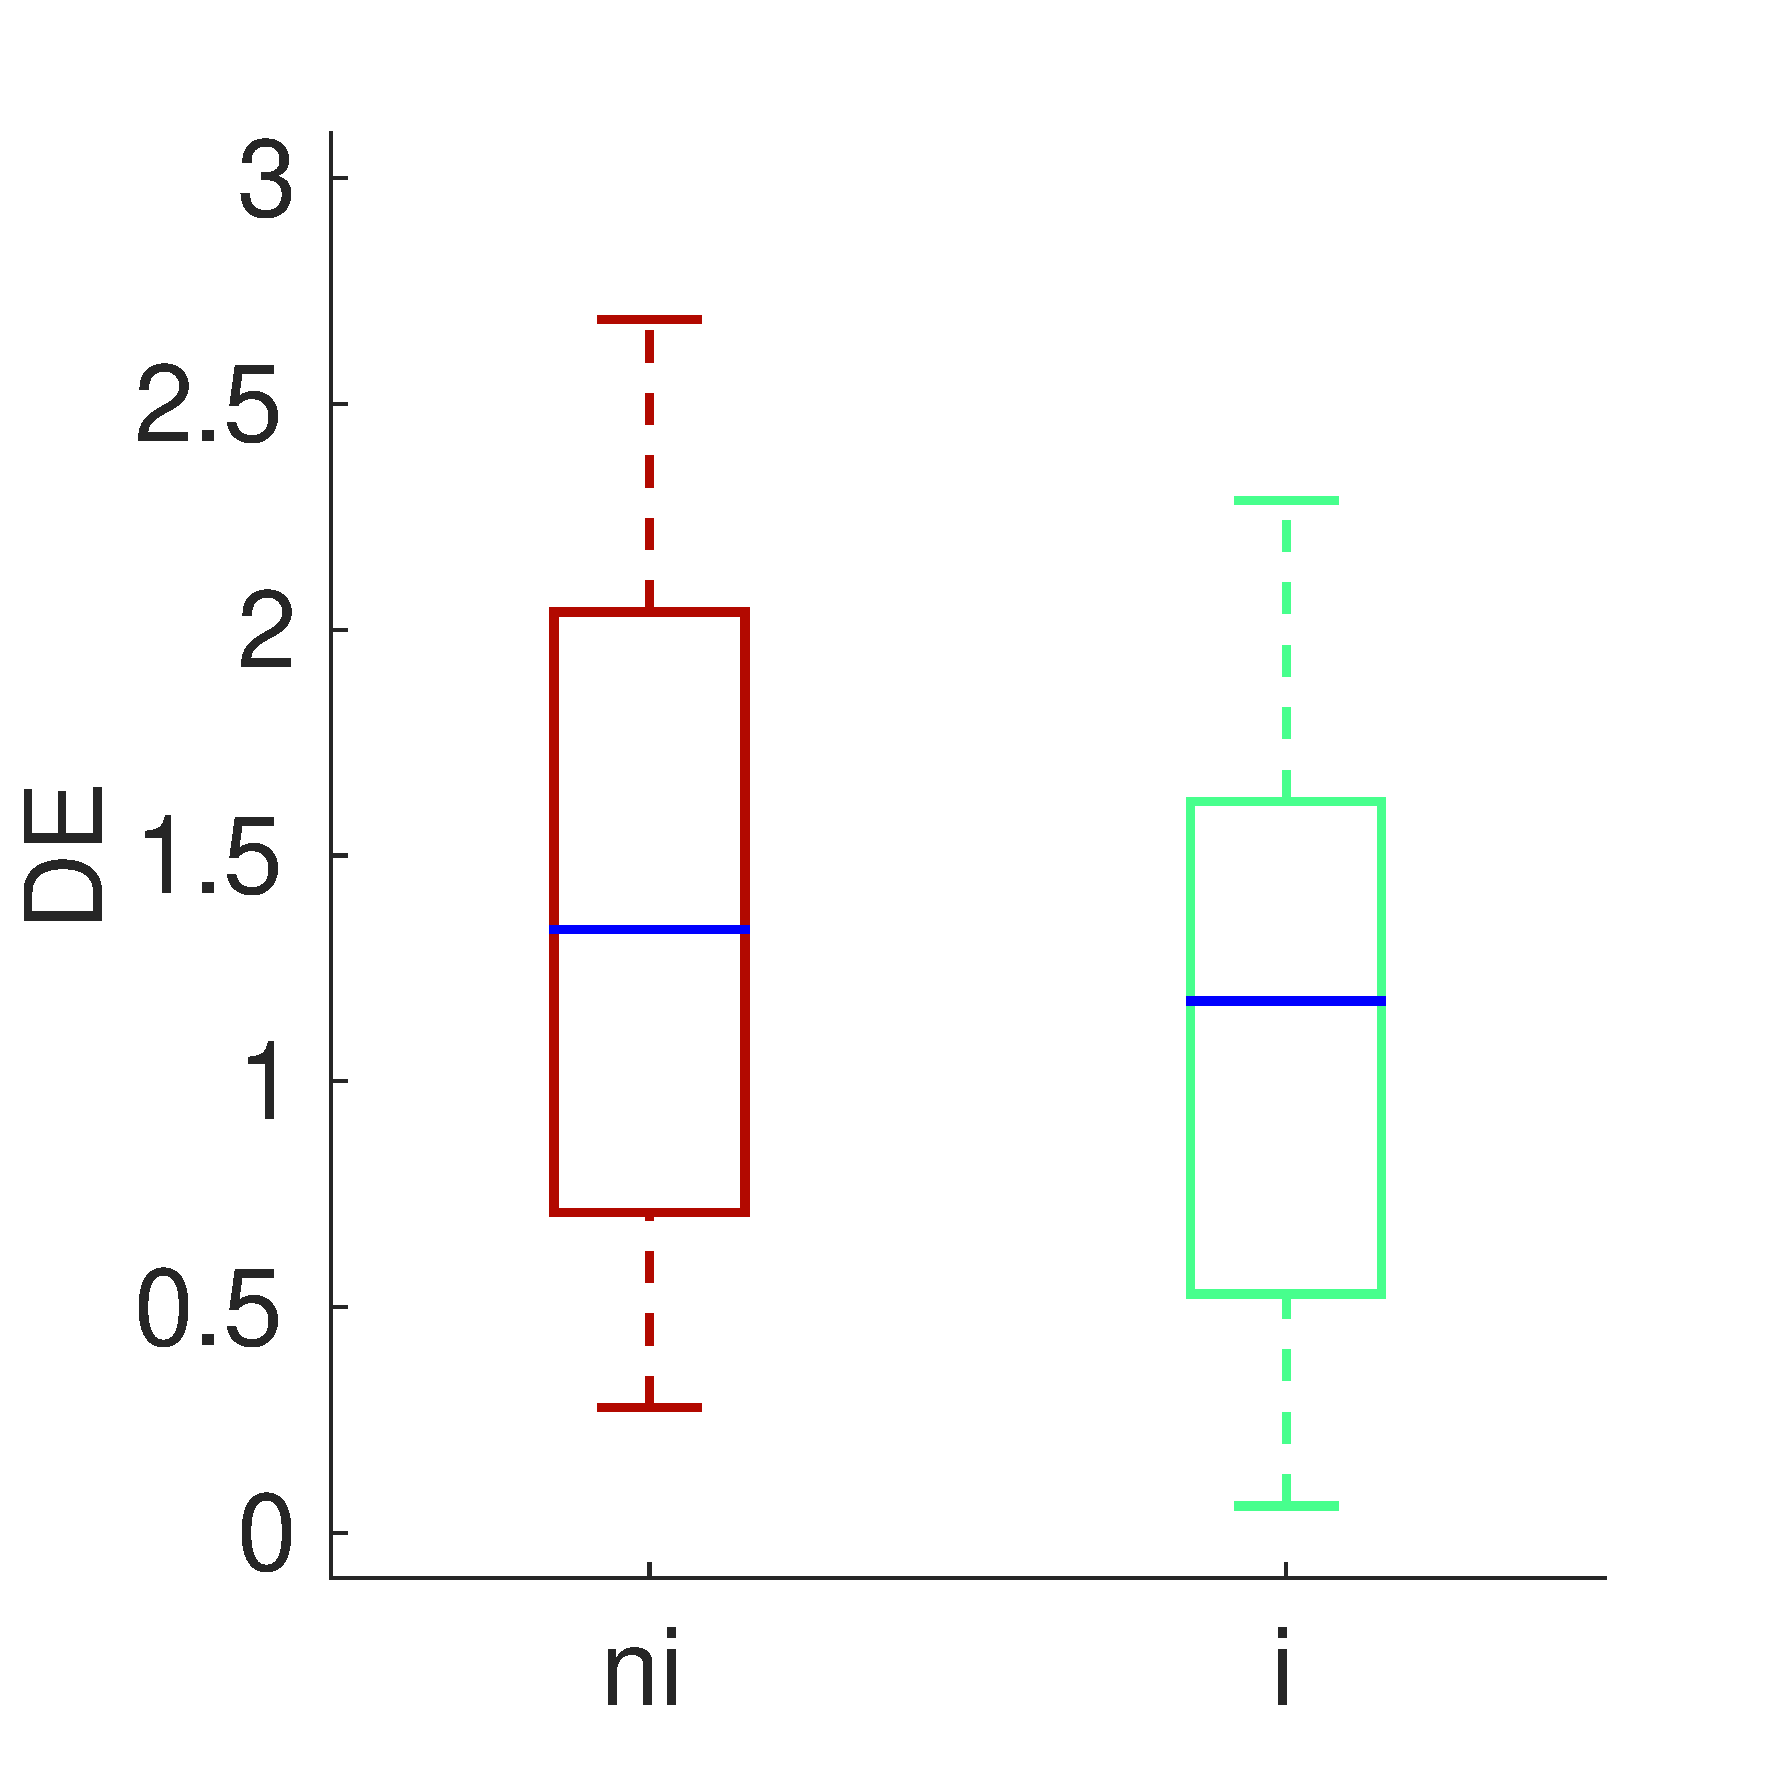
\includegraphics[width=.33\linewidth]{gfxXpUrbanSoundscape/xp_density_3}\label{fig:densityb}}\par
        \subfloat[]
        {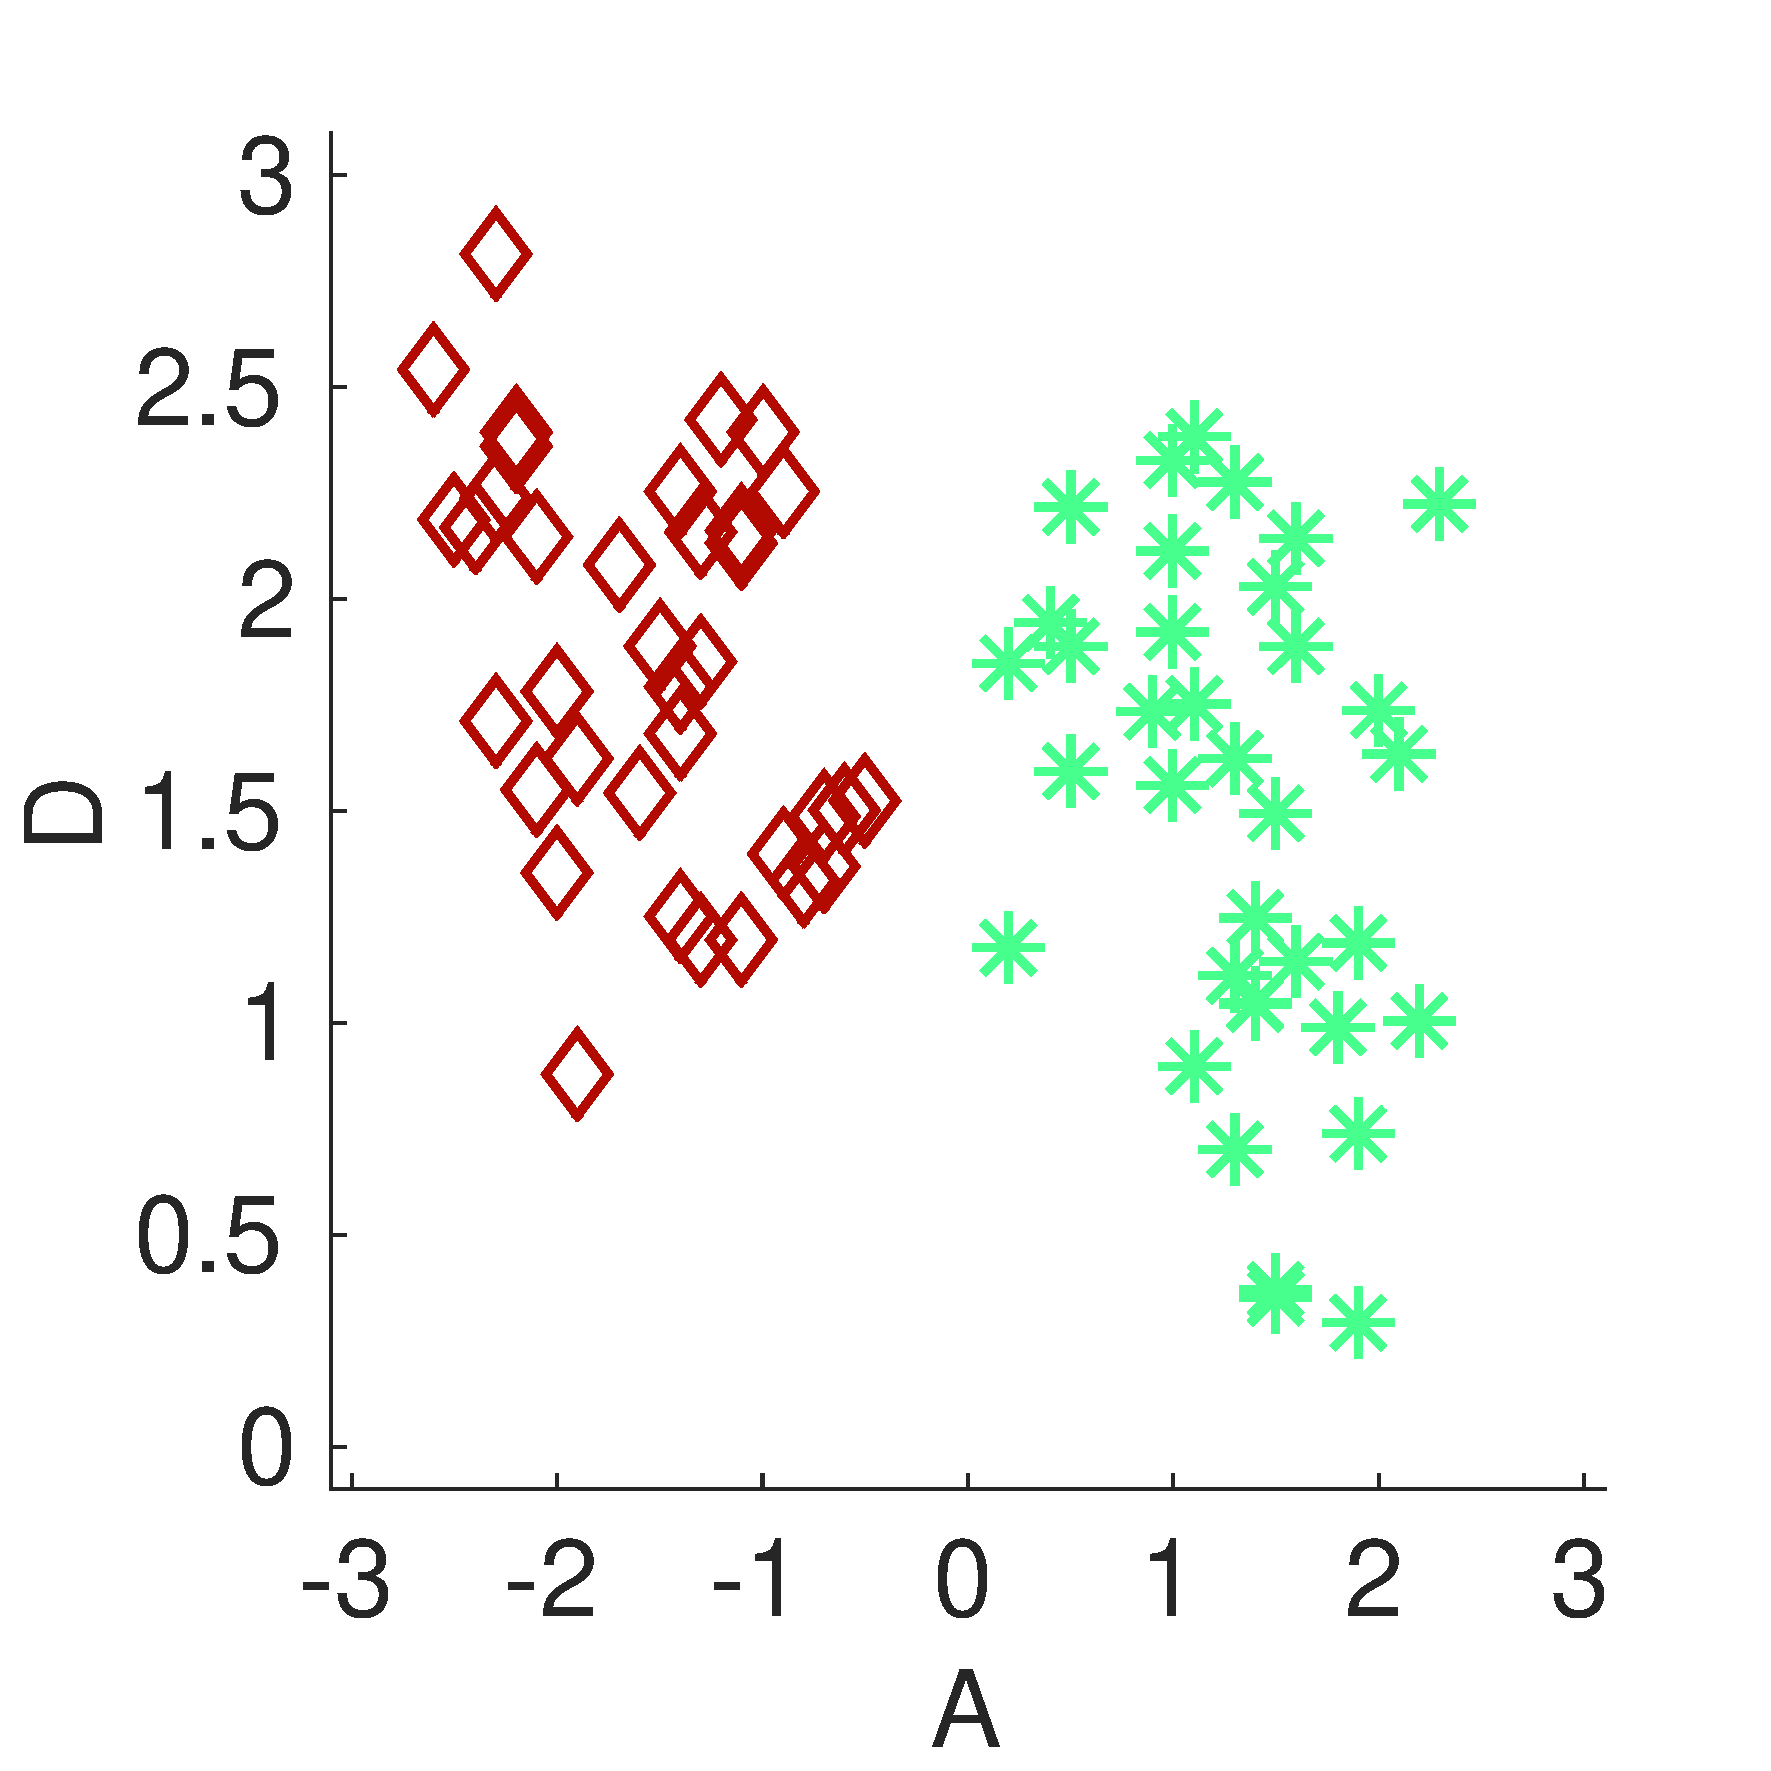
\includegraphics[width=.33\linewidth]{gfxXpUrbanSoundscape/xp_density_2}\label{fig:densityc}}
        \subfloat[]
        {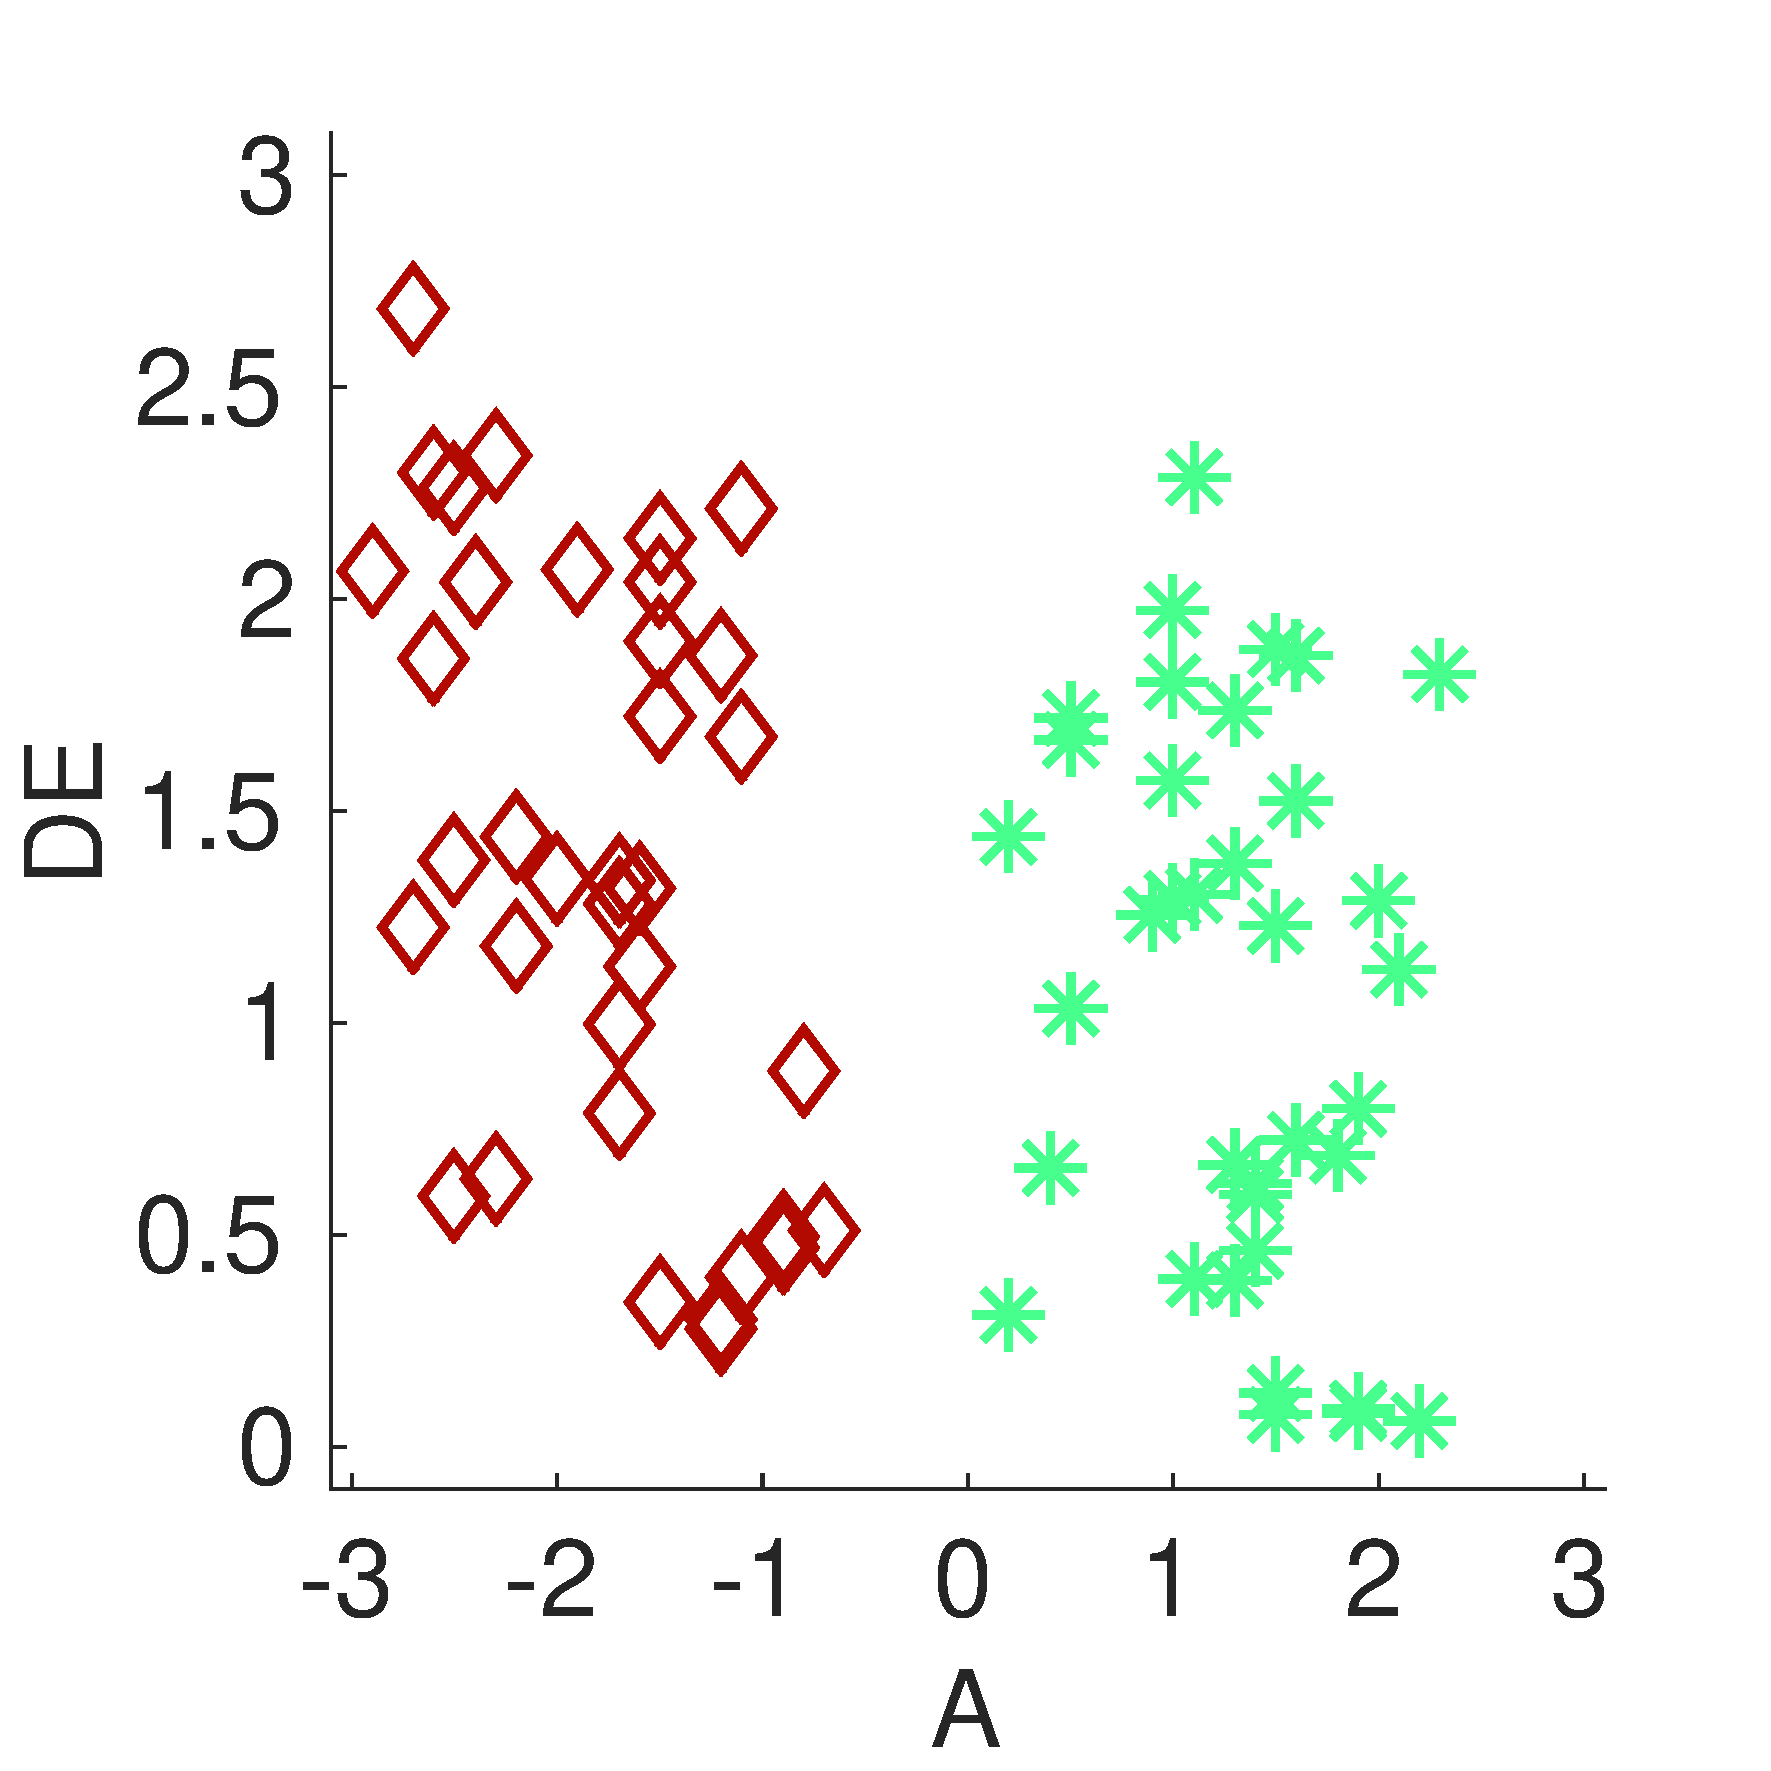
\includegraphics[width=.33\linewidth]{gfxXpUrbanSoundscape/xp_density_4}\label{fig:densityd}}
       \caption[TODO]{TODO}\label{fig:density}
\end{figure}

\begin{figure}[t]
        \myfloatalign
        \includegraphics[width=.8\linewidth]{gfxXpUrbanSoundscape/xp1_div_1}
       \caption[TODO]{TODO}\label{fig:diversity}
\end{figure}

\subsection{Influence des descripteurs structurels sur l'agrément perçu}
\label{sec:ch5_corrDesStruct}

Nous analysons, dans cette section, les relations fines qui peuvent exister entre les descripteurs structurels, d'une part, et l'agrément perçu, d'autre part. Contrairement à la section précédente, où la qualité affective des scènes est représentée de manière binaire (i \vs~ni), nous considérons, ici, l'agrément moyen $\mathcal{A}_{scene}$ comme descripteur perceptif. Il s'agit d'étudier l'existence de potentielles corrélations entre les descripteurs structurels et $\mathcal{A}_{scene}$. Les coefficients de corrélations linéaires calculés entre $\mathcal{A}_{scene}$ \vs~$L$, $L(E)$, $L(T)$, $D$, $D(E)$ et $DIV(E)$ sont présentés dans le tableau~\ref{tab:corrStructA}. Les relations entre $\mathcal{A}_{scene}$ et les descripteurs structurels sont illustrées par les figures~\ref{fig:soundleveld},~\ref{fig:soundlevele} et ~\ref{fig:soundlevelf}, pour les niveaux sonores, et les figures~\ref{fig:densityc} et~\ref{fig:densityd}, pour les densités. 

Concernant $L$, on observe une forte corrélation négative ($r=-0.77$, $p<0.01$) avec $\mathcal{A}_{scene}$, indiquant que plus le niveau sonore est élevé, plus la scène est désagréable. Cependant, la figure~\ref{fig:soundleveld} suggère que cette relation ne s'opère pas de la même manière pour les i- et ni-scènes. En effet, la corrélation entre $L$ et $\mathcal{A}_{scene}$, pour les ni-scènes, reste élevée ($r=-0.78$, $p<0.01$), mais est inexistante pour les i-scènes. 

Cette corrélation élevée, considérant l'ensemble des scènes, résulte du fait que les i-scènes ont tendance à être moins fortes que les ni-scènes, donnant ainsi l'illusion de prolonger la corrélation négative observée pour les ni-scènes.  

Nous en concluons que $L$:

\begin{itemize}
\item permet bien de faire la distinction entre les i- et ni-scènes,
\item permet de finement caractériser l'agrément perçu des ni-scènes,
\item n'est pas un indicateur pertinent de l'agrément perçu pour des environnements a priori agréables.
\end{itemize}

Les mêmes observations sont faites concernant $L(E)$ (\cf~\ref{fig:soundlevele}). Pour $L(T)$ (\cf~\ref{fig:soundlevelf}), bien que, à considérer l'ensemble des scènes, on observe une corrélation modérée, cela n'est pas vérifié quand on regarde séparément les i-scènes ($r=-0.33$, $p=0.05$) et les ni-scènes ($r=-0.00$, $p=0.99$). Là encore on peut penser que la corrélation négative observée pour l'ensemble des scènes est un artefact, résultant du fait que le niveau des textures des i-scènes a tendance à être plus bas que celui des ni-scènes. Ainsi, si les événements sonores conservent une certaine capacité de prédiction de l'agrément pour les ni-scènes, le niveau des textures n'apporte, lui, que peu d'informations, quel que soit l'environnement.

Considérant l'ensemble des scènes, nous observons une corrélation négative faible pour $D$ ($r=-0.44$, $p<0.01$) et $D(E)$ ($r=-0.34$, $p<0.01$). Une relation semblable est observée pour les ni-scènes ($D$: $r=-0.38$, $p<0.05$; $D(E)$: $r=-0.46$, $p<0.01$), mais aucune corrélation n'est observée pour les i-scènes. La densité de sources sonores semble donc avoir un faible impact sur l'agrément perçu, si l'on considère les ni-scènes, mais, comme pour les niveaux, cette densité ne semble pas avoir d'impact pour les i-scènes.

En ce qui concerne la diversité des classes d'événements, une corrélation négative faible est observée pour les niveaux d'abstraction 1, 2 et 3, en tenant compte de l'ensemble des scènes. Si l'on considère les i- et ni-scènes séparément, aucune corrélation significative n'est trouvée. Les conclusions sont similaires à celles faites pour $L(T)$: la diversité permet uniquement de faire la distinction entre les deux types d'environnements, mais ne permet pas de caractériser précisément l'agrément perçu.

En résumé, en présence d'un environnement désagréable, les niveaux sonores, en particulier ceux des événements, ainsi que, dans une moindre mesure, la densité de sources présentes, ont un impact négatif sur l'agrément. En présence d'un environnement agréable, aucun des descripteurs structurels considérés ici ne semble influer sur la perception de l'agrément. 

Ces premiers résultats pourraient montrer qu'il existe deux modes de perception, mobilisant chacun des descripteurs indépendants, modes qui s'activent en fonction de la nature de l'environnement (i ou ni).

Le fait qu'aucun des descripteurs globaux ne permettent de caractériser l'agrément des i-scènes peut nous amener à penser que toutes les sources sonores ne contribuent pas de manière égale à la perception de l'agrément, mais, que seules les caractéristiques de certaines d'entre elles ont une réelle influence. Afin d'approfondir ce point, nous analysons, dans la section suivante, les scènes d'un point de vue sémantique, \ie~en nous intéressant à la nature des sources qui les composent. \\


\begin{table}[t]
\centering
\begin{tabular}{l c c c} 
            & ensemble                     & i-scènes                   & ni-scènes    \\
\hline
$L$            & \textbf{-0.77} ($p<0.01$)    & -0.32 ($p=0.06$)           & \textbf{-0.78} ($p<0.01$)\\
$L(E)$         & \textbf{-0.75} ($p<0.01$)    & -0.20 ($p=0.24$)           & \textbf{-0.75} ($p<0.01$)\\
$L(T)$         & \textbf{-0.53} ($p<0.01$)    & -0.33 ($p=0.05$)           &  -0.00 ($p=0.99$) \\
$D$            & \textbf{-0.43} ($p<0.01$)    & -0.31 ($p=0.07$)           & \textbf{-0.38} ($p<0.05$)\\
$D(E)$         & \textbf{-0.34} ($p<0.01$)    & -0.22 ($p=0.21$)           & \textbf{-0.46} ($p<0.01$)\\
$DIV(E)$ 0     &          -0.07 ($p=0.52$)    & -0.25 ($p=0.15$)           & -0.23 ($p=0.23$)\\
$DIV(E)$ 1     & \textbf{-0.47} ($p<0.01$)    & -0.25 ($p=0.14$)           & -0.26 ($p=0.13$)\\
$DIV(E)$ 2     & \textbf{-0.41} ($p<0.01$)    & -0.21 ($p=0.22$)           & -0.25 ($p=0.14$)\\
$DIV(E)$ 3     & \textbf{-0.37} ($p<0.01$)    & -0.18 ($p=0.30$)           & -0.18 ($p=0.16$)\\
\hline
\end{tabular}
\vspace{0.5mm}
\caption{Coefficients de corrélation linéaire calculés entre l'agrément perçu moyen $\mathcal{A}_{scene}$ \vs~TODO}
\label{tab:corrStructA}
\end{table}

\subsection{Étude comparative entre les descripteurs sémantiques}

\subsubsection{Analyse qualitative}
\label{sec:ch5_anaQualiSem}

Nous analysons la composition des scènes en comptant le nombre de sujets ayant utilisé une classe de sons pour simuler un type d'environnements. Les résultats sont présentés à la figure~\ref{fig:soundsourcea} pour les événements, et à la figure~\ref{fig:soundsourceb} pour les textures. Par souci d'espace, nous choisissons un niveau d'abstraction intermédiaire entre le niveau 0 et 1, noté $0+$, pour représenter les classes (\cf~Figure~\ref{fig:taxonomie}).

Nous observons une différence notable dans le choix des classes entre les i- et ni-scènes. La répartition des classes est très proche de celle obtenue dans une étude similaire sur les environnements sonores urbains idéaux \citep{guastavino2006ideal}, \ie~les classes suggérant la présence humaine et la nature sont très présentes dans les i-scènes, a contrario, les classes désignant des sons mécaniques et/ou de travaux sont principalement utilisées pour les ni-scènes.

Ces résultats confirment un fait déjà observé: la nature sémantique des sources sonores joue un rôle prédominant dans l'appréciation de l'environnement \citep{raimbault2005urban,dubois2006cognitive}.

Nous notons quelques différences avec \citep{guastavino2006ideal}: les résultats obtenus par Guastavino montrent que les sons de \emph{transports publics} sont caractéristiques des environnements sonores urbains idéaux. Les auteurs attribuent cela au fait que la perception de l'agrément est, entre autre, soumise à un contexte socio-culturel. Dans notre représentation du monde, les sons de transports publics sont positivement connotés, et ont ainsi tendance à être mieux acceptés que les sons de véhicules privés.

Dans une certaine mesure, nos résultats contredisent ce fait. La figure~\ref{fig:soundsourcea} montre, en effet, que les classes d'événements de \emph{transports publics} (\emph{bus} et \emph{train}, \cf~Figure~\ref{fig:soundsourcec}) ont été utilisées par les sujets, pour des i-scènes, dans $28\%$ des cas, et pour des ni-scènes, dans $42\%$ des cas. Les résultats ne remettent pas en question le fait que les sons de \emph{transports publics} soient bien acceptés: $25\%$ des sujets ont utilisé la classe \emph{bus} pour les i-scènes, un chiffre comparable à celui de la classe \emph{Vélo}, et bien supérieur à celui de toute autre classe de véhicules privés. Cependant les classes \emph{transports publics} sont également bien présentes dans les ni-scènes, plus que les classes \emph{voiture} ou \emph{camion} par exemple. La classe \emph{transports publics} ne peut donc pas être considérée comme typique d'un environnement sonore urbain idéal.

Cette différence peut s'expliquer par la nature des deux protocoles expérimentaux utilisés. Comme nous l'avons fait, Guastavino demande à ses sujets de décrire un environnement en se basant sur leurs mémoires. Mais, contrairement à nous, ils ne disposent pas de supports sonores. Le fait que nos sujets soient confrontés à la réalité acoustique des sons, pour recréer leurs environnements, peut avoir pour effet de diminuer l'impact du contexte socio-culturel. D'autres études utilisant des sons comme stimuli montrent que la classe \emph{bus} peut avoir un effet négatif sur l'appréciation de l'environnement \citep{lavandier2006contribution}.

\begin{figure}[t]
        \myfloatalign
        \subfloat[]
        {\includegraphics[width=.8\linewidth]{gfxXpUrbanSoundscape/xp1_class_1}\label{fig:soundsourcea}} \par
        \subfloat[]
        {\includegraphics[width=.4\linewidth]{gfxXpUrbanSoundscape/xp1_class_2}\label{fig:soundsourceb}} 
        \subfloat[]
        {\includegraphics[width=.4\linewidth]{gfxXpUrbanSoundscape/xp1_class_3}\label{fig:soundsourcec}} 
       \caption[TODO]{TODO}\label{fig:soundsource}
\end{figure}

\subsubsection{Marqueurs sonores}

Nous avons mis en évidence que, qualitativement, la composition des sources sonores des scènes diffère selon les types d'environnements (i ou ni). Nous essayons de voir maintenant si, parmi ces classes, certaines sont typiques d'un environnement en particulier. Pour ce faire, nous utilisons le V-test (\cf~Section~\ref{sec:ch5_methodoEtStat1}), en considérant séparément chaque niveau d'abstraction. Les résultats sont présentés dans le tableau~\ref{tab:markers}.

Concernant les événements sonores, 9 marqueurs sont identifiés sur l'ensemble des niveaux d'abstraction. Comme la figure~\ref{fig:soundsource} le laissait présager, les classes relatives à l'activité humaine (\emph{pas homme béton}, \emph{sonnette vélo}), et à la nature (\emph{animaux, oiseaux}, \emph{chants d'oiseaux}) sont des marqueurs de i-scènes. Nous notons également la présence de la classe \emph{cloche} dans les marqueurs d'un environnement idéal. Ce fait est possiblement dû au \emph{background} socio-culturel des sujets, dans leur grande majorité, des citoyens européens. En effet, selon Schafer, un son reconnu par un individu comme faisant partie intégrante de son environnement est bien accepté. Les marqueurs de ni-scènes sont des classes faisant référence à des sons de travaux (\emph{travaux}), ou suggérant un trafic dense (\emph{klaxon}, \emph{sirène}).

Concernant les textures sonores, 5 marqueurs sont identifiés. Pour les i-scènes, il s'agit de classes faisant référence à des ambiances amorphes, calmes, (\emph{cour-intérieur/parc} et \emph{parc}). Pour les ni-scènes, il s'agit, comme pour les événements, de classes faisant référence à des bruits de travaux (\emph{travaux} et \emph{véhicule de travaux}), ainsi que d'une classe faisant référence au trafic (\emph{carrefour}).


\gl{Bien que l'ensemble des marqueurs identifiés soient intuitifs, aucune des classes d'événements faisant directement référence aux bruits de véhicules motorisés n'est un marqueur, exception faite de la classe de texture \emph{carrefour}}. Pour représenter un trafic désagréable, les sujets ont porté leurs choix sur les classes \emph{klaxon} et \emph{sirène}. On peut supposer que les sons isolés de véhicules sont compris comme faisant partie intégrante de l'environnement urbain, et ne sont donc pas particulièrement associés à un environnement désagréable. \\ 

\gl{TODO: ici analyse des caractéristiques des classes trafics} \\
\gl{TODO: ici reprendre les conclusions de \citep{lavandier2006contribution} et \citep{ricciardi2015sound}}

\begin{table}[t]
 \setlength{\tabcolsep}{0.2pt}
 \centering
  {\renewcommand{\arraystretch}{0.9}
\begin{tabular}{c c c c} 
Niveau        & \multicolumn{2}{c}{Marqueurs sonores événements} \\
d'abstraction & i-scènes & ni-scènes \\
\hline
0  &                               &  construction work (3.78)  \\
\hline
  & church bell  (4.5)             & horn  (3.9) \\
1 & bell bike    (4.3)             & siren (3.9)\\
  & animal       (4.2)             &       \\
   \hline
  & birds        (4.8)             & horn  (4.0)\\
2 & church bell  (4.4)             & siren (4.0)\\
  & bell bike    (4.2)             &       \\
   \hline
  & birds singing (4.8)            & horn  (4.1)\\
  & church bell   (4.3)            & siren (4.0)\\
3 & bell bike     (4.2)            &       \\
  & male footsteps                 &  \\
  &   concrete (3.6)               &  \\
  &                                & \\ 
  & \multicolumn{2}{c}{Marqueurs sonores textures}      \\
  & i-scènes & ni-scènes \\
\hline
0 &     courtyard/park (4.1)       &  construction work (3.9)  \\
\hline
1 &     park (3.65)                &  crossroads (3.6)  \\
  &                                &  vehicle work (3.3)  \\
\hline
2 &     park (3.64)                &  crossroads (3.56)  \\
\hline
\end{tabular}
}
\vspace{0.5mm}
\caption[Classes d'événements identifiées comme étant des marqueurs sonores]{Classes d'événements identifiées comme étant des marqueurs sonores. Dans chaque cellule, les marqueurs sont ordonnés par ordre décroissant de valeur $V$.}
\label{tab:markers}
\end{table}

\subsection{Étude des espaces de représentation induits par les descripteurs sémantiques}

Dans cette partie, nous évaluons la capacité d'une représentation sémantique à séparer les deux types d'environnements. Pour ce faire, nous calculons une précision au rang 5 ($p@5$) sur l'espace induit par les descripteurs sémantiques $S$, et ce pour chaque niveau d'abstraction (\cf~Section~\ref{sec:ch5_methodoEtStat1}). Les vecteurs $S$ sont construits en utilisant toutes les classes ($ET$), les classes d'événements ($E$), les classes de textures ($T$), les classes d'événements ne considérant que les marqueurs sonores ($E_m$), les classes d'événements ne considérant pas les marqueurs sonores $E_{w/o,m}$. Les résultats sont affichés sur la figure~\ref{fig:pa5}.

En ce qui concerne $ET$, la $p@5$ est de $76\%$ pour le niveau d'abstraction 0, et reste supérieure à $86\%$ à partir du niveau d'abstraction 1. Ces résultats confirment qu'il est possible de clairement distinguer les deux types d'environnements en se basant seulement sur la présence ou l'absence des classes de sons. Nous notons également que, plus le niveau d'abstraction est élevé, plus la capacité de séparer les environnements est importante. En d'autres termes, plus nous sommes précis dans notre description de la composition des scènes, plus nous sommes à même d'établir une distinction claire entre les i- et ni-scènes.

En considérant séparément $E$ et $T$, il apparaît que 1) la $p@5$ obtenue avec $E$ est similaire à celle obtenue avec $ET$, et 2) que la $p@5$ obtenue avec $T$ est systématiquement inférieure d'environ $10$ à $15\%$ à celle de $E$. Ces résultats indiquent que l'information sémantique permettant de séparer les deux environnements est principalement portée par les événements. Ces résultats font, par ailleurs, écho aux travaux de  \citep{maffiolo_caracterisation_1999}, qui montrent que nous analysons de manière descriptive (en identifiant les sources) les scènes événementielles, \ie~composées d'événements sonores (\cf~Section~\ref{sec:ch3_catsoundscape}).

Enfin, il apparaît que la $p@5$ obtenue avec $E_{m}$ est similaire, voire supérieure à celles de $E$ et $ET$, et ce bien qu'une information partielle soit utilisée dans ce cas pour décrire les scènes. La dimension des vecteurs de description $S$ pour $E_m$ est en effet inférieure à la dimension des vecteurs $S$ pour $E$, qui est elle même inférieure à celle obtenue dans le cas où toutes les classes sont utilisées ($ET$). De plus, dans le cas où les marqueurs ne sont pas pris en compte pour la description ($E_{w/o,m}$), les résultats chutent, passant même en dessous de ceux obtenus en ne considérant que les textures. Cela confirme que la majorité de l'information sémantique permettant de faire la distinction entre i-scènes et ni-scènes est incluse dans les marqueurs.

En résumé, nous déduisons de cette analyse les points suivants:

\begin{enumerate}
\item contrairement à ce que nous avions constaté avec les descripteurs structurels, une description sémantique de la composition des scènes, en terme de présence/absence de sources sonores, permet de bien distinguer les deux types d'environnements (i ou ni);
\item l'information sémantique est majoritairement portée par les classes d'événements sonores;
\item parmi les classes d'événements, seule une partie, \ie~les marqueurs sonores, sont nécessaires afin de faire la distinction entre les i- et ni-scènes.
\end{enumerate}

Maintenant que nous avons isolé les classes typiques des i- et ni-scènes, et vérifié que la distinction entre ces environnements dépendait de la présence de ces classes, il reste à voir si une description structurelle des scènes, basée uniquement sur ces marqueurs sonores, permet de caractériser l'agrément perçu, mieux qu'une description structurelle globale. \\

\gl{analyse marqueur texture ?}\\
\gl{HCA sur $S$, + ANOVA sur $\mathcal{A}_{scene}$}

\begin{figure}[t]
        \myfloatalign
        \includegraphics[width=.8\linewidth]{gfxXpUrbanSoundscape/pa5_1}
       \caption[TODO]{TODO}\label{fig:pa5}
\end{figure}

\subsection{L'influence spécifique des marqueurs sonores sur l'agrément perçu}

\begin{table}[t]
\centering
\begin{tabular}{l r r} 
                  &   i-scenes                  & ni-scenes \\
\hline
$L_m$              & 0.03  ($p=0.88$)           & \textbf{-0.75} ($p<0.01$) \\
$L(E)_m$           & 0.08  ($p=0.66$)           & \textbf{-0.71} ($p<0.01$) \\
$L(T)_m$           & -0.11 ($p=0.66$)           & -0.17 ($p=0.37$) \\
$L_b$              & \textbf{-0.52} ($p<0.01$)  & -0.32 ($p=0.06$) \\
$L(E)_b$           & \textbf{-0.51} ($p<0.01$)  & -0.30 ($p=0.07$) \\
$L(T)_b$           & -0.32 ($p=0.05$)           & \textbf{-0.73} ($p<0.01$) \\
$L_m-L_b$          & \textbf{0.67} ($p<0.01$)   & -0.31 ($p=0.07$) \\
$L(E)_m-L(E)_b$    & \textbf{0.66} ($p<0.01$)   & -0.28 ($p=0.10$) \\
$L(T)_m-L(T)_b$    & 0.16 ($p=0.54$)            & 0.21 ($p=0.28$) \\
$D_m$              & 0.03 ($p=0.85$)            & -0.31 ($p=0.07$) \\
$D(E)_m$           & 0.09 ($p=0.62$)            & \textbf{-0.44} ($p<0.01$) \\
\hline
\end{tabular}
\vspace{0.5mm}
\caption{Coefficients de corrélation linéaire calculés entre l'agrément perçu moyen $\mathcal{A}_{scene}$ \vs~TODO.}
\label{tab:corrMarkers}
\end{table}

Comme pour la  section~\ref{sec:ch5_corrDesStruct}, nous évaluons les corrélations entre $\mathcal{A}_{scene}$ et les descripteurs structurels. Pour cette section, les descripteurs structurels sont calculés en tenant compte des marqueurs sonores précédemment identifiés. Nous définissons $X_m$ le descripteur $X$ calculé en ne prenant en compte que les sons des marqueurs. A l'inverse, nous définissons $X_b$ ($b$: pour ``\,bruit\,'') le descripteur $X$ calculé en prenant en compte toutes les classes de sons excepté les marqueurs. Lorsque le descripteur caractérise une i-scène (idem pour une ni-scène), nous ne considérons, pour le calcul, que les marqueurs identifiés pour les i-scènes (ou pour les ni-scènes), que nous nommons i-marqueurs (ou ni-marqueurs). Les résultats sont affichés sur le tableau~\ref{tab:corrMarkers}.

Considérons dans un premier temps les densités (\cf~Figures~\ref{fig:densityMarker}). Les résultats pour $D_m$ et $D(E)_m$ sont similaires à ceux observés précédemment pour $D$ et $D(E)$, a l'exception de $D_m$  qui ne présente plus une corrélation significative pour les ni-scènes. Ces résultats tendent à confirmer que la densité est un indicateur d'agrément de faible importance, qu'on la considère globalement, ou en prenant en compte les contributions séparées de différentes sources. \\

\gl{TODO: Rajouter $D_b$} \\

Concernant les niveaux sonores (\cf~Figures~\ref{fig:soundlevelMarker}), là encore les mêmes tendances sont observées entre $L_m$, $L(E)_m$ et $L(T)_m$, d'une part, et $L$, $L(E)$ et $L(T)$, d'autre part. Que l'on considère uniquement les marqueurs, ou l'ensemble des classes, il s'avère que :

\begin{enumerate}
\item Il existe une différence significative entre les niveaux des i- et ni-scènes ($L_m$, $L(E)_m$ et $L(T)_m$: $p<0.01$) 
\item Le niveau sonore des scènes est majoritairement porté par les événements sonores.
\item Le niveau sonore des événements a une influence sur la perception de l'agrément pour les ni-scènes, mais pas pour les i-scènes.
\item Le niveau sonore des textures ne joue aucun rôle dans la perception de l'agrément
\end{enumerate}

En conclusion, le niveau des ni-marqueurs a une influence négative sur l'agrément pour les ni-scènes, en revanche le niveau des i-marqueurs n’impacte pas l'agrément perçu pour les i-scènes.

En considérant maintenant les classes non marqueurs  (\cf~Figures~\ref{fig:soundlevelNoise}), nous remarquons, sur les i-scènes, une corrélation négative modérée/faible pour $L_b$  ($r=-52$, $p<0.01$) et $L(E)_b$ ($r=-51$, $p<0.01$). C'est la première fois qu'un indicateur objectif nous permet de préciser l'agrément des environnements agréables. Ceci nous amène à conclure que le niveau des classes de sons n'étant pas typiques d'un environnement agréable a un impact négatif sur l'agrément. 

Par ailleurs, alors que $L(T)$ ne présentait pas de corrélation pour les ni-scènes, une corrélation négative forte est observée pour $L(T)_b$ ($r-0.73$, $p<0.01$). Ce fait indique que des classes de textures, utilisées pour simuler aussi bien les i-scènes que les ni-scènes, n'affectent pas l'agrément perçu de la même manière. Pour une même classe \emph{foule}, le niveau perçu dans un cadre idéal n'affectera pas la perception de l'agrément, alors que dans un cadre non-idéal, il impactera négativement le ressenti \gl{TODO: chiffre}.

Pour finir, nous considérons un dernier groupe de descripteurs, nommément $L_m-L_b$, $L(E)_m-L(E)_b$ et $L(T)_m-L(T)_b$ (\cf~Figures~\ref{fig:soundlevelMarkerDiff}). Ces descripteurs expriment la différence entre les niveaux des marqueurs, et ceux des autres classes de sons. Ils traduisent l'émergence des marqueurs par rapport à la mixture sonore.

Pour les i-scènes, une corrélation modéré et positive est observée pour $L_m-L_b$ ($r=0.67$, $p<0.01$) et $L(E)_m-L(E)_b$ ($r=0.66$, $p<0.01$). Pour les ni-scènes, aucune corrélation n'est observée. Dans le cas des i-scènes, ce n'est donc pas le niveau absolu des marqueurs qui importe, mais leur niveau relatif, par rapport aux autres sons qui composent la scène. On observe donc pour les environnements idéaux un double mécanisme perceptif: 

\begin{itemize}
\item plus le niveau absolu des sons n'étant pas des i-marqueurs est élevé, plus l'agrément est faible,
\item plus le niveau relatif des i-marqueurs, par rapport aux autres sons, est élevé, plus l'agrément est élevé.
\end{itemize}

Pour les ni-scènes, le fait que nous observions des corrélations pour $L_m$ et $L(E)_m$, et aucune pour $L_m-L_b$ et $L(E)_m-L(E)_b$, montre que c'est bien le niveau absolu qui importe.

\begin{figure}[t]
        \myfloatalign
        \subfloat[]
        {\includegraphics[width=.33\linewidth]{gfxXpUrbanSoundscape/xp_density_7}\label{fig:densityMarkera}}
        \subfloat[]
        {\includegraphics[width=.33\linewidth]{gfxXpUrbanSoundscape/xp_density_9}\label{fig:densityMarkerb}}\par
        \subfloat[]
        {\includegraphics[width=.33\linewidth]{gfxXpUrbanSoundscape/xp_density_8}\label{fig:densityMarkerc}}
        \subfloat[]
        {\includegraphics[width=.33\linewidth]{gfxXpUrbanSoundscape/xp_density_10}\label{fig:densityMarkerd}}
       \caption[TODO]{TODO}\label{fig:densityMarker}
\end{figure}

\begin{figure}[t]
        \myfloatalign
        \subfloat[]
        {\includegraphics[width=.33\linewidth]{gfxXpUrbanSoundscape/xp_soundlevel_7}\label{fig:soundlevelMarkera}}
        \subfloat[]
        {\includegraphics[width=.33\linewidth]{gfxXpUrbanSoundscape/xp_soundlevel_11}\label{fig:soundlevelMarkerb}}
        \subfloat[]
        {\includegraphics[width=.33\linewidth]{gfxXpUrbanSoundscape/xp_soundlevel_15}\label{fig:soundlevelMarkerc}}\par
        \subfloat[]
        {\includegraphics[width=.33\linewidth]{gfxXpUrbanSoundscape/xp_soundlevel_8}\label{fig:soundlevelMarkerd}}
        \subfloat[]
        {\includegraphics[width=.33\linewidth]{gfxXpUrbanSoundscape/xp_soundlevel_12}\label{fig:soundlevelMarkere}}
        \subfloat[]
        {\includegraphics[width=.33\linewidth]{gfxXpUrbanSoundscape/xp_soundlevel_16}\label{fig:soundlevelMarkerf}}       
        \caption[TODO]{TODO}\label{fig:soundlevelMarker}
\end{figure}

\begin{figure}[t]
        \myfloatalign 
        \subfloat[]
        {\includegraphics[width=.33\linewidth]{gfxXpUrbanSoundscape/xp_soundlevel_9}\label{fig:soundlevelNoisea}}
        \subfloat[]
        {\includegraphics[width=.33\linewidth]{gfxXpUrbanSoundscape/xp_soundlevel_13}\label{fig:soundlevelNoiseb}}
        \subfloat[]
        {\includegraphics[width=.33\linewidth]{gfxXpUrbanSoundscape/xp_soundlevel_17}\label{fig:soundlevelNoisec}}\par
        \subfloat[]
        {\includegraphics[width=.33\linewidth]{gfxXpUrbanSoundscape/xp_soundlevel_10}\label{fig:soundlevelNoised}}
        \subfloat[]
        {\includegraphics[width=.33\linewidth]{gfxXpUrbanSoundscape/xp_soundlevel_14}\label{fig:soundlevelNoisee}}
        \subfloat[]
        {\includegraphics[width=.33\linewidth]{gfxXpUrbanSoundscape/xp_soundlevel_18}\label{fig:soundlevelNoisef}}
       \caption[TODO]{TODO}\label{fig:soundlevelNoise}
\end{figure}

\begin{figure}[t]
        \myfloatalign 
        \subfloat[]
        {\includegraphics[width=.33\linewidth]{gfxXpUrbanSoundscape/xp_soundlevel_19}\label{fig:soundlevelMarkerDiffa}}
        \subfloat[]
        {\includegraphics[width=.33\linewidth]{gfxXpUrbanSoundscape/xp_soundlevel_21}\label{fig:soundlevelMarkerDiffb}}
        \subfloat[]
        {\includegraphics[width=.33\linewidth]{gfxXpUrbanSoundscape/xp_soundlevel_23}\label{fig:soundlevelMarkerDiffc}}\par
        \subfloat[]
        {\includegraphics[width=.33\linewidth]{gfxXpUrbanSoundscape/xp_soundlevel_20}\label{fig:soundlevelMarkerDiffd}}
        \subfloat[]
        {\includegraphics[width=.33\linewidth]{gfxXpUrbanSoundscape/xp_soundlevel_22}\label{fig:soundlevelMarkerDiffe}}
        \subfloat[]
        {\includegraphics[width=.33\linewidth]{gfxXpUrbanSoundscape/xp_soundlevel_24}\label{fig:soundlevelMarkerDifff}}
       \caption[TODO]{TODO}\label{fig:soundlevelMarkerDiff}
\end{figure}




\subsection{Discussions}

Dans cette expérience, nous identifions 6 indicateurs structurels globaux permettant de distinguer, de manière globale, les environnements sonores idéaux et non-idéaux.

\begin{itemize}
\item niveau sonore: calculé sur tous les sons $L$, les événements $L(E)$ et les textures $L(T)$; 
\item densité: calculée de manière globale $D$ et sur les événements $D(E)$;
\item diversité: calculée uniquement sur les événements $DIV(E)$.
\end{itemize}

Parmi ces indicateurs structurels, seuls $L$ et $LE$ permettent de prédire l'agrément. Nous notons cependant que cette prédiction ne vaut que pour les ni-scènes. 

Nous observons qu'une description sémantique des scènes, basée sur la présence/absence des classes de sons, permet de bien prédire la nature de l'environnement. Par ailleurs, il apparaît qu'il est possible d'obtenir une prédiction similaire, voire meilleure, en ne considérant qu'un sous groupe de classes d'événements,\ie~les marqueurs sonores.

Parmi les descripteurs structurels spécifiques, calculés en tenant compte des marqueurs sonores, plusieurs permettent maintenant de faire la distinction entre les i-scènes et ni-scènes:

\begin{itemize}
\item \gl{TODO}.
\end{itemize}

Parmi ces descripteurs, 8 semblent impacter l'agrément perçu: 

\begin{itemize}
\item $L_b$ et $L(E)_b$ ont un impact négatif sur les i-scènes;
\item $L(E)_m-L(E)_b$ et $L_m-L_b$ ont un impact positif sur les i-scènes;
\item $L_m$, $L(E)_m$, $L(T)_b$ et $D(E)_m$ ont un impact négatif les ni-scènes.
\end{itemize}

De cette analyse, nous retenons les points suivants:

\begin{itemize}
\item \emph{distinguer les i- et ni-scènes}: Les descripteurs sémantiques, ainsi que certains descripteurs structurels globaux, permettent de faire la distinction entre les i-scènes et les ni-scènes. La description sémantique semble être plus performante;
\item \emph{événements ou textures}: Que ce soit pour les descripteurs sémantiques ou structurels, c'est majoritairement les événements qui permettent de distinguer les deux types d'environnements, les textures n'apportant, au mieux, qu'une information limitée;
\item \emph{prédire l'agrément}: Si l'on considère une description fine de l'agrément, il semble que la manière de percevoir la qualité de l'environnement diffère en fonction de la nature de ce dernier (i ou ni). Il n'apparaît pas envisageable de considérer un même jeu de descripteurs pour prédire, à la fois, l'agrément des i-scènes, et l'agrément des ni-scènes. Pour les ni-scènes, ce sont le niveau global ($L$ et $L(E)$), la densité globale ($D$ et $D(E)$), et/ou le niveau des marqueurs sonores ($L_m$ et $L$), qui impactent négativement l'agrément. On note ici que prendre en compte les contributions de différentes sources n'améliore pas la capacité de prédiction de l'agrément, par rapport à une analyse holistique de l'environnement. Pour les i-scènes, par contre, prédire l'agrément requiert d'étudier, de manière séparée, les caractéristiques des marqueurs sonores, et celles de l'ensemble des autres sons. Ainsi, le niveau des marqueurs relatifs au bruit est positivement corrélé à l'agrément, alors que le niveau du bruit est, lui, négativement corrélé.  
\end{itemize}

L'existence de deux modes de perception, mobilisant différents types de descripteurs, et dépendant de la nature du stimuli, est un phénomène qui a déjà été observé pour la perception des textures (\cf~Section~\ref{sec:ch3_eventTexture}). Le cerveau adapte sa manière de traiter l'information (résumé statistique pour les textures, description fine pour les événements) suite à une prise de décision antérieure quant à la nature du stimuli (à savoir ``\,est-ce un événement ou une texture ?\,''). De la même manière, les indicateurs actifs dans le jugement de l'agrément dépendent, eux aussi, d'une identification préalable de la nature hédonique globale de l'environnement (idéale ou non idéale).

Ces résultats peuvent potentiellement influer sur les stratégies à adopter pour améliorer la qualité de l’environnement sonore:

\begin{itemize}
\item dans le cadre de scènes non-idéales, il s'agit de diminuer le niveau sonore, soit de manière globale, soit en agissant sur certaines sources (\emph{sirène}, \emph{klaxon});
\item dans le cadre de scènes idéales, il s'agit 1) d'identifier les sons agréables, \ie~les marqueurs sonores, 2) de baisser le niveau des autres sons, 3) voire, en restant dans la limite du raisonnable, d'augmenter le niveau des marqueurs par rapport aux autres sons.
\end{itemize}

Nous montrons que les descripteurs à utiliser dépendent de la nature de l'environnement, et que cette nature est elle même dépendante de la composition sémantique, \ie~des sources sonores présentes. Dans une certaine mesure, nous pouvons donc dire que les descripteurs dépendent des sources sonores présentes. Mais nous observons également que le type de descripteurs à utiliser, pour une même source, varie en fonction de la nature de l'environnement \gl{TODO: développer sur le contexte environnemental pour l'agrément, reprendre l'exemple de \emph{foule}}. \\

\gl{TODO: Reprendre la conclusion de l'article et Proposer un modèle perceptif sur la base du modèle prédictif}
\gl{TODO, l'utilisation de trafic reprendre les conclusions de \citep{lavandier2006contribution}}
\gl{TODO, les résultats (2 modes d'obs) concordent avec les observations faites pas \citep{ricciardi2015sound} (\cf~Section~\ref{XX}).}

\section[Modification de la composition sémantique]{Agir sur l'agrément perçu en modifiant la composition sémantique}
\label{sec:xp3}

\subsection{Objectif}

L'expérience précédente à montré que, parmi les classes de sons peuplant le monde sonore, certaines, les marqueurs, sont caractéristiques de certains types d'environnements. Ces marqueurs sonores semblent avoir un impact particulier sur la perception de leurs environnements. C'est ce dernier point qui est étudié dans cette expérience.

Afin de vérifier que l'agrément des scènes idéales et non-idéales dépend de la présence des marqueurs, les scènes sonores précédemment simulées sont régénérées, sans les classes de marqueurs. Pour les i-scènes, seules les i-marqueurs sont omis, de même, pour les ni-scènes, seuls les ni-marqueurs sont retirés. Une épreuve d'évaluation de l'agrément, dont le protocole se rapproche de celui de l'expérience 1.b, est alors conduite.

L'objectif est de vérifier si l'absence des marqueurs a un impact sur l'agrément perçu. Deux hypothèses sont formulées:

\begin{itemize}
\item \emph{pour les ni-scènes} nous faisons l'hypothèse que l'absence des ni-marqueurs va \textbf{augmenter} la valeur de l'agrément perçu;
\item \emph{pour les i-scènes} nous faisons l'hypothèse que l'absence des i-marqueurs va \textbf{diminuer} la valeur de l'agrément perçu.
\end{itemize}

Si la première hypothèse est intuitive, la deuxième l'est moins. En effet, il n’apparaît pas évident que la suppression des i-marqueurs, bien que s'agissant de sons positivement connotés, diminue la qualité globale d'un environnement. Cette suppression aura, de surcroît, pour effet de diminuer le niveau sonore global de la scène. 

Néanmoins, comme nous l'avons vu, le niveau global n'est qu'un indicateur partiel de l'agrément pour les environnements sonores idéaux. Qui plus est, cet indicateur, lorsque qu'il décrit le niveau des i-marqueurs, impacte de manière positive la qualité de la scène. L'hypothèse mérite donc d'être vérifiée.

\subsection{Planification expérimentale}

Nous nommons cette expérience: \emph{expérience 2}. \\

\textbf{Banque de données} \\

La banque de données de stimuli compte 144 séquences de 30 secondes. Ces 144 séquences comprennent:

\begin{itemize}
\item \emph{72 am-scènes}: les 72 scènes précédemment simulées, incluant les classes de marqueurs (am). Nous notons i/am-scenes, les 36 scènes idéales comprenant les marqueurs, et ni/am-scènes les 36 scènes non-idéales comprenant les marqueurs;
\item \emph{72 sm-scènes}: les 72 scènes précédemment simulées, régénérées sans les classes de marqueurs (sm). Nous notons i/sm-scenes, les 36 scènes idéales générées sans les marqueurs, et ni/sm-scènes les 36 scènes non-idéales générées sans les marqueurs.
\end{itemize}


Nonobstant l'absence des marqueurs, les am- et sm-scènes sont en tout point semblables. Nombre de am-scènes sont composées, en majorité, de samples de marqueurs. Afin de pas abusivement dénaturer ces scènes, en créant notamment des temps de ``\,vide\,'', \ie~ne comprenant aucun sample, nous ne supprimons que les marqueurs des classes d'événements du premier niveau d'abstraction (\cf~Tableau~\ref{tab:markers}). Ces classes sont: 

\begin{itemize}
\item \emph{cloche}, \emph{sonnette de vélo}, \emph{animaux};
\item \emph{sirène}, \emph{klaxon}.
\end{itemize}
 
Il est important de noter ici que tous les i- et ni-marqueurs ne sont donc pas supprimés dans les sm-scènes. \\
 
\textbf{Procédure} \\

Les sujets évaluent les 144 scènes. L'évaluation s'effectue sur une échelle sémantique bipolaire de 11 points allant de -5 (non-idéale/très désagréable) à +5 (idéale/très agréable). Avant de noter une scène, les sujets doivent obligatoirement en écouter les 20 premières secondes. Après la notation, ils sont libres de passer à la scène suivante.

Pour chaque sujet, les scènes sont présentées dans un ordre aléatoire. Les 10 premières scènes permettent au sujet de calibrer ses notes. Elles sont obligatoirement composées de 5 i/am-scènes et de 5 ni/am-scènes. Ces 10 premières scènes sont rejouées à la fin de l'expérience, et seules les notes données à la deuxième occurrence sont prises en compte. 

L'expérience est prévue pour durer 1 heure. Les sujets ne connaissent pas la nature des scènes.\\

\textbf{Apparatus} \\

Tous les sujets passent l'expérience sur des machines identiques (\gl{description des machines}). L'audio est diffusé en stéréophonie, par le biais de casques audio semi-ouvert \emph{Beyer-Dynamic DT 990 Pro}. Toutes les scènes sonores ont été re-simulées sur la base des partitions obtenues lors de l'expérience de simulation. Le niveau sonore de sortie est identique pour tous les sujets.

Tous les sujets réalisent l'expérience simultanément, dans un environnement calme. Ils n'ont pas le droit de s'adresser la parole pendant l'expérience. 

Un expérimentateur est présent durant la totalité de l'expérience, afin de contrôler le bon déroulement de cette dernière, et de répondre aux éventuelles questions des sujets.  \\

\textbf{Participants} \\

12 sujets (4 femmes) participent à l'expérience. Aucun d'entre eux n'a réalisé l'expérience de simulation, ni la première expérience d'évaluation. Les sujets sont âgés de 22 à 61 ans (moyenne: 29.5, écart-type: 14). Tous les sujets vivent dans un milieu urbain.

Tous les sujets ont réalisé l'expérience avec succès.

\subsection{Données et méthodes d'analyses}

\subsubsection{Nature des données analysées}

Les données analysées sont les mêmes que pour la première expérience. Nous invitons le lecteur à se référer à la section~\ref{sec:ch5_dataType1} pour plus de détails.
 
\subsubsection{Méthodologie et Outils statistiques}
\label{sec:ch5_methodoEtStat2}

L'expérience aborde trois problématiques:

\begin{itemize}
\item \emph{influence des descripteurs structurels des scènes avec marqueurs sur l'agrément perçu: une analyse comparative}: les 72 am-scènes utilisées par l'expérience 1.b étant ré-évaluées lors de cette expérience, il est donc possible de réaliser une étude comparative entre les expériences 1.b et 2, afin de vérifier la cohérence des résultats obtenus lors de l'expérience 1.b. Les méthodes d'analyse appliquées sont identiques à celles de l'expérience 1.b (\cf~Section~\ref{sec:ch5_methodoEtStat1});
\item \emph{influence de la présence des marqueurs sur l'agrément perçu}: il s'agit ici de vérifier que la suppression des i- et ni-marqueurs impacte l'agrément perçu. Pour ce faire, nous utilisons l'analyse de variance (\cf~Annexe~\ref{app:anova}). Nous considérons, comme variable dépendante,  $\mathcal{A}_{sujet}$, et, comme variables indépendantes, le type d'environnement (i/ni), et la présence/absence de marqueurs (am/sm). Chaque sujet devant évaluer la totalité des stimuli, une ANOVA à mesures répétées à deux facteurs (\cf~Annexe~\ref{app:anova}) est utilisée afin vérifier s'il existe des différences significatives d'agrément perçu. Les deux variables indépendantes sont considérées comme des facteurs \emph{within-subject} (\cf~Annexe~\ref{app:anova}). Les facteurs n'étant composés que de deux niveaux chacun (type: i/ni; marqueur: am/sm), l'hypothèse de sphéricité n'a pas besoin d'être vérifiée. Les analyses \emph{post hoc} sont conduites en appliquant la procédure de Bonferroni;
\item \emph{influence des descripteurs structurels des sm-scènes sur l'agrément perçu}: il s'agit là d'étudier l'agrément en fonction des indicateurs structurels des scènes. Dans un premier temps, nous vérifions que l'agrément moyen de chaque type de scènes (i, ni, am et sm) varie significativement. Une analyse de variance est pratiquée, avec, comme variable dépendante,  $\mathcal{A}_{scene}$, et, comme variables indépendantes, le type d'environnement (i/ni), et la présence/absence de marqueurs (am/sm). Dans cette analyse, les observations considérées sont les scènes. Comme il existe une dépendance entre les am et sm-scènes, une ANOVA mixte est utilisée, comprenant, comme facteur \emph{within-subject}, la présence/absence de marqueurs, et comme facteur \emph{between-subject}, le type d'environnement. Les analyses \emph{post hoc} sont conduites en appliquant la procédure de Bonferroni. Dans un second temps, comme pour l'expérience 1.b, nous étudions l'existence de relations linéaires entre les descripteurs structurels des sm-scènes et $\mathcal{A}_{scene}$. Pour mesurer la corrélation, nous utilisons le coefficient de Pearson (\cf~Annexe~\ref{app:statuni}).
\end{itemize}

Tous les tests de significativité sont effectués avec un seuil critique $\alpha=0.05$.

\subsection{Détection de valeurs extrêmes}

Considérons $\mathcal{A}_{sujet}$ pour les am-scènes (\cf~Figure~\ref{fig:xp4_note_2}). Il apparaît que les réponses du sujet 7 diffèrent des autres. Comme observé sur la figure~\ref{fig:xp4_note_1} (\cf~Figure~\ref{fig:xp4_note_1g} pour le sujet 7), ce dernier à évalué positivement les ni/am-scènes. Le sujet 7 a donné à 58\% des ni/am-scènes une note supérieure à 0,  contre une moyenne de 11\% pour les autres sujets. De plus, le sujet 7 a utilisé l'ambitus maximal (-5 à 5) pour noter à la fois les i/ et ni/am-scènes. Ces faits n'ayant pas été observés pour les autres sujets, que l'on considère les expériences 2 ou 1.b, le sujet 7 est éliminé de l'analyse. 

\begin{figure}[t]
        \myfloatalign
        \subfloat[sujet 1]
        {\includegraphics[width=.16\linewidth]{gfxXpUrbanSoundscape/xp4_note_1}\label{fig:xp4_note_1a}}
        \subfloat[sujet 2]
        {\includegraphics[width=.16\linewidth]{gfxXpUrbanSoundscape/xp4_note_2}\label{fig:xp4_note_1b}}
        \subfloat[sujet 3]
        {\includegraphics[width=.16\linewidth]{gfxXpUrbanSoundscape/xp4_note_3}\label{fig:xp4_note_1c}}
        \subfloat[sujet 4]
        {\includegraphics[width=.16\linewidth]{gfxXpUrbanSoundscape/xp4_note_4}\label{fig:xp4_note_1d}}
        \subfloat[sujet 5]
        {\includegraphics[width=.16\linewidth]{gfxXpUrbanSoundscape/xp4_note_5}\label{fig:xp4_note_1e}}
        \subfloat[sujet 6]
        {\includegraphics[width=.16\linewidth]{gfxXpUrbanSoundscape/xp4_note_6}\label{fig:xp4_note_1f}}\par       
        \subfloat[sujet 7]
        {\includegraphics[width=.16\linewidth]{gfxXpUrbanSoundscape/xp4_note_7}\label{fig:xp4_note_1g}}
        \subfloat[sujet 8]
        {\includegraphics[width=.16\linewidth]{gfxXpUrbanSoundscape/xp4_note_8}\label{fig:xp4_note_1h}}
        \subfloat[sujet 9]
        {\includegraphics[width=.16\linewidth]{gfxXpUrbanSoundscape/xp4_note_9}\label{fig:xp4_note_1i}}
        \subfloat[sujet 10]
        {\includegraphics[width=.16\linewidth]{gfxXpUrbanSoundscape/xp4_note_10}\label{fig:xp4_note_1j}}
        \subfloat[sujet 11]
        {\includegraphics[width=.16\linewidth]{gfxXpUrbanSoundscape/xp4_note_11}\label{fig:xp4_note_1h}}
        \subfloat[sujet 12]
        {\includegraphics[width=.16\linewidth]{gfxXpUrbanSoundscape/xp4_note_12}\label{fig:xp4_note_1l}}       
        \caption[TODO]{TODO}\label{fig:xp4_note_1}
\end{figure}


\begin{figure}[t]
        \myfloatalign
        \subfloat[]
        {\includegraphics[width=.33\linewidth]{gfxXpUrbanSoundscape/xp4_note_13}\label{fig:xp4_note_2}}
        \subfloat[]
        {\includegraphics[width=.33\linewidth]{gfxXpUrbanSoundscape/xp4_note_15}\label{fig:xp4_note_4}}
        \subfloat[]
        {\includegraphics[width=.33\linewidth]{gfxXpUrbanSoundscape/xp4_note_16}\label{fig:xp4_note_5}}
       \caption[TODO]{TODO}\label{fig:xp4_note_245}
\end{figure}


\subsection{Influence des descripteurs structurels des scènes avec marqueurs sur l'agrément perçu: une analyse comparative}

Cette section présente une étude comparative entre les résultats de l'expérience 1.b, et ceux obtenus, pour les am-scènes,dans l'expérience ci-après. 

Nous commençons par évaluer la corrélation entre les $\mathcal{A}_{scene}$ obtenues par les deux études. Les résultats sont affichés sur la figure~\ref{fig:xp4_note_5}. La corrélation est élevée, que l'on considère l'ensemble des scènes ($r=0.98$, $p<0.01$), ou les i- ($r=0.82$, $p<0.01$), ou encore les ni-scènes  ($r=0.91$, $p<0.01$).

Concernant les différences de $\mathcal{A}_{sujet}$ entre les i/am- et ni/am-scenes, nous observons un delta net et significatif ($p<0.01$), avec une différence moyenne des écarts de 4.5. Ces résultats sont en accord avec ceux de l'expérience 1.b.

Comme pour l'expérience 1.b, une analyse des relations entre les descripteurs structurels et $\mathcal{A}_{scene}$ est réalisée. Les résultats sont affichés dans le tableau~\ref{tab:corrAmXP4}. Ce tableau fait apparaître des différences: 

Considérons les niveaux ($L$, $L(E)$ et $L(T)$) pour les i-scènes. Une corrélation modérée négative est observée entre ces descripteurs et $\mathcal{A}_{scene}$, alors qu'aucune n'était observée pour l'expérience 1.b. Il apparaît, dans l'expérience 2, que ces descripteurs ont joué un rôle (négatif) plus important dans l'évaluation des qualités affectives des scènes, que dans l'expérience 1.b. Cependant, l'observation précédemment faite, sur le fait que ces descripteurs n'impactent pas de la même manière la perception des i et ni-scènes, se maintient. En effet les corrélations pour les niveaux restent modérées pour les i-scènes ($r<-0.46$), alors que celles observées pour les ni-scènes sont toutes élevées ($r>-0.81$). Le niveau est donc bien pris en compte dans l'évaluation des i-scènes, mais moins que dans l'évaluation des ni-scènes. Cette recrudescence de l'importance du niveau est également observée sur $L_b$ pour les ni-scènes ($r=-0.40$, $p<0.05$), ainsi que sur $L(T)_b$ ($r=-0.46$, $p<0.01$) pour les i-scènes, mais là encore les corrélations reste modérées voire faibles.

Deux différences concernant les densités sont relevées. Nous observons une corrélation modérée sur $D$ pour les i-scènes ($r=-0.42$, $p<0.05$) et une corrélation faible pour $D(E)$ ($r=-0.42$, $p<0.05$). Comme pour le niveau, la densité semble avoir une influence plus importante dans l'expérience 2. 

La majorité des différences concerne les descripteurs des i-scènes. Pour tous ces descripteurs, les corrélations observées pour les ni-scènes sont plus importantes pour l'expérience 2 que pour l'expérience 1.b. Considérant les différences d'appréciation entre les i- et ni-scènes, les résultats restent donc consistant. Il apparaît que les descripteurs structurels de niveaux et de densités ont globalement plus influé sur l'agrément perçu dans l'expérience 2 que dans l'expérience 1.b.

Excepté ces points, tous les résultats observés dans les deux études concordent, notamment:

\begin{itemize}
\item l'effet bénéfique de l'émergence des i-marqueurs d'événements pour les i-scènes ($L_m-L_b$: $r=0.60$, $p<0.01$; $L(E)_m-L(E)_b$: $r=0.56$, $p<0.01$);
\item l'effet négatif des ni-marqueurs d'événements pour les ni-scènes ($L_m$: $r=0.75$, $p<0.01$; $L(E)_m$: $r=0.73$, $p<0.01$);
\item l'impact nul des marqueurs de textures pour les i- ($L(T)_m$: $r=-0.05$, $p=0.86$) et ni-scènes ($L(T)_m$: $r=-0.06$, $p=0.76$).
\end{itemize}


\gl{TODO: compléter}

\begin{table}[t]
\centering
\begin{tabular}{l r r} 
                   &   i-scènes                      & ni-scènes \\
\hline
$L$                & \textbf{-0.46$^{*}$} ($p<0.01$) & \textbf{-0.83} ($p<0.01$)\\
$L(E)$             & -0.33 ($p=0.05$)                & \textbf{-0.84} ($p<0.01$)\\
$L(T)$             & \textbf{-0.42$^{*}$} ($p<0.05$) &  0.04 ($p=0.81$) \\
$D$                & \textbf{-0.42$^{*}$} ($p<0.05$) & \textbf{-0.47} ($p<0.01$)\\
$D(E)$             & \textbf{-0.36$^{*}$} ($p<0.05$) & \textbf{-0.57} ($p<0.01$)\\
$DIV(E)$ 0         & -0.26 ($p=0.13$)                & -0.32 ($p=0.06$)\\
$DIV(E)$ 1         & -0.29 ($p=0.10$)                & -0.31 ($p=0.06$)\\
$DIV(E)$ 2         & -0.24 ($p=0.17$)                & -0.32 ($p=0.06$)\\
$DIV(E)$ 3         & -0.20 ($p=0.25$)                & -0.31 ($p=0.06$)\\
$L_m$              & 0.16  ($p=0.36$)                & \textbf{-0.75} ($p<0.01$) \\
$L(E)_m$           & 0.08  ($p=0.64$)                & \textbf{-0.73} ($p<0.01$) \\
$L(T)_m$           & -0.05 ($p=0.86$)                & -0.06 ($p=0.76$) \\
$L_b$              & \textbf{-0.64} ($p<0.01$)       & \textbf{-0.40$^{*}$} ($p<0.05$) \\
$L(E)_b$           & \textbf{-0.57} ($p<0.01$)       & -0.33 ($p=0.05$) \\
$L(T)_b$           & \textbf{-0.46$^{*}$} ($p<0.01$) & \textbf{-0.83} ($p<0.01$) \\
$L_m-L_b$          & \textbf{0.60} ($p<0.01$)        & -0.25 ($p=0.14$) \\
$L(E)_m-L(E)_b$    & \textbf{0.56} ($p<0.01$)        & -0.27 ($p=0.11$) \\
$L(T)_m-L(T)_b$    & 0.43 ($p=0.07$)                 & 0.36 ($p=0.05$) \\
$D_m$              & -0.12 ($p=0.48$)                & -0.33 ($p=0.05$) \\
$D(E)_m$           & -0.21 ($p=0.22$)                & \textbf{-0.53} ($p<0.01$) \\
\hline
\end{tabular}
\vspace{0.5mm}
\caption{\gl{TODO: i/am-scenes et ni/am-scenes}}
\label{tab:corrAmXP4}
\end{table}

\subsection{Influence de la présence des marqueurs sur l'agrément perçu}
\label{sec:ch5_Asujet}

Dans cette section nous étudions comment les sujets ont perçu les différents types de scènes, nommément: i/am-, ni/am-, i/sm- et ni/sm-scène. L'ANOVA à mesures répétées pratiquée sur $\mathcal{A}_{sujet}$ (\cf~Figure~\ref{fig:xp4_note_2}) montre un effet significatif du type d'environnements (i/ni: $F[1,10]=175$, $p<0.01$), de la présence/absence des marqueurs (am/sm: $F[1,10]=7$, $p<0.05$) , ainsi que de l'interaction entre les deux facteurs ($F[1,10]=67$, $p<0.01$).

L'analyse \emph{post hoc} montre, quant à elle, des différences significatives entre tous les groupes d'observations, notamment entre les i/am- et i/sm-scenes ($p<0.05$) et les ni/am- et ni/sm-scenes ($p<0.01$).


Ces résultats indiquent que la suppression des événements a effectivement modifié la perception des scènes par les sujets. Nos deux hypothèses sont ainsi vérifiées:

\begin{itemize}
\item la suppression des ni-marqueurs a amélioré les qualités perçues des ni-scènes;
\item la suppression des i-marqueurs a diminué les qualités perçues des i-scènes.
\end{itemize}

L'interaction significative montre que l'effet du type d'environnements influe sur l'effet dû à l'absence/présence des marqueurs. En effet la moyenne des écarts entre les am- et sm-scènes est plus importante pour les ni-scènes (1.1) que pour les i-scènes (0.5). 

Les i-marqueurs ont donc bien un effet bénéfique sur la perception d'un environnement. Le fait que leur suppression diminue $\mathcal{A}_{scene}$ montre clairement qu'il est possible d'améliorer la qualité d'un environnement en ajoutant des sons bien acceptés comme \emph{oiseaux}. Ces conclusions vont dans le sens de l'approche positive comme introduite par Schafer \citep{schafer1977tuning} (\cf~Section~\ref{sec:ch3_urbanNoiseSoundscape}). \\

\gl{TODO: citation}

\subsection{Influence des descripteurs structurels des scènes sans marqueurs sur l'agrément perçu}

L'ANOVA mixte pratiquée sur $\mathcal{A}_{scene}$ (\cf~Figure~\ref{fig:xp4_note_4}) montre un effet significatif du type d'environnements (i/ni: $F[1,70]=222$, $p<0.01$), de la présence/absence des marqueurs (am/sm: $F[1,70]=5$, $p<0.05$) , ainsi que de l'interaction entre les deux facteurs ($F[1,70]=35$, $p<0.01$).

L'analyse \emph{post hoc} montre des différences significatives entre tous les groupes d'observations, notamment, là encore, entre les i/am- et i/sm-scenes ($p<0.05$) et les ni/am- et ni/sm-scenes ($p<0.01$).

Ainsi, les quatre types de scènes, considérant $\mathcal{A}_{scene}$ comme indicateur, forment bien quatre groupes distincts. L'interaction montre que le type d'environnement impacte l'effet provoqué par la suppression des marqueurs, les moyennes d'écart étant identiques à celles de l'analyse de la section précédente (ni-scènes: 1.1,  i-scènes: 0.5, \cf~Section~\ref{sec:ch5_Asujet}).
 
\begin{table}[t]
\centering
\begin{tabular}{l c c c} 
               & ensemble                     & i-scènes                   & ni-scènes    \\
\hline
$L$            & \textbf{-0.79} ($p<0.01$)    & \textbf{-0.49} ($p<0.01$)  & \textbf{-0.74} ($p<0.01$)\\
$L(E)$         & \textbf{-0.76} ($p<0.01$)    & \textbf{-0.44} ($p<0.01$)  & \textbf{-0.70} ($p<0.01$)\\
$L(T)$         & \textbf{-0.41} ($p<0.01$)    & -0.17 ($p=0.36$)           & -0.44 ($p=0.80$) \\
$D$            & \textbf{-0.49} ($p<0.01$)    & -0.31 ($p=0.07$)           & -0.29 ($p=0.08$)\\
$D(E)$         & \textbf{-0.45} ($p<0.01$)    & -0.29 ($p=0.09$)           & \textbf{-0.39} ($p<0.05$)\\
$DIV(E)$ 0     &         -0.10  ($p=0.40$)    & -0.26 ($p=0.13$)           & -0.32 ($p=0.06$)\\
$DIV(E)$ 1     & \textbf{-0.49} ($p<0.01$)    & -0.29 ($p=0.09$)           & -0.31 ($p=0.06$)\\
$DIV(E)$ 2     & \textbf{-0.43} ($p<0.01$)    & -0.24 ($p=0.17$)           & -0.32 ($p=0.06$)\\
$DIV(E)$ 3     & \textbf{-0.39} ($p<0.01$)    & -0.20 ($p=0.25$)           & -0.32 ($p=0.06$)\\
\hline
\end{tabular}
\vspace{0.5mm}
\caption{\gl{TODO: i/sm-scenes et ni/sm-scenes}}
\label{tab:corrSmXP4}
\end{table}

\begin{figure}[t]
        \myfloatalign
        \includegraphics[width=.8\linewidth]{gfxXpUrbanSoundscape/xp4_div_1}
        \caption[TODO]{TODO}\label{fig:diversitySansMarker}
\end{figure}

\begin{figure}[t]
        \myfloatalign
        \subfloat[]
        {\includegraphics[width=.33\linewidth]{gfxXpUrbanSoundscape/xp4_density_13}\label{fig:densitySansMarkera}}
        \subfloat[]
        {\includegraphics[width=.33\linewidth]{gfxXpUrbanSoundscape/xp4_density_15}\label{fig:densitySansMarkerb}}\par
        \subfloat[]
        {\includegraphics[width=.33\linewidth]{gfxXpUrbanSoundscape/xp4_density_14}\label{fig:densitySansMarkerc}}
        \subfloat[]
        {\includegraphics[width=.33\linewidth]{gfxXpUrbanSoundscape/xp4_density_16}\label{fig:densitySansMarkerd}}
       \caption[TODO]{TODO}\label{fig:densitySansMarker}
\end{figure}

\begin{figure}[t]
        \myfloatalign
        \subfloat[]
        {\includegraphics[width=.33\linewidth]{gfxXpUrbanSoundscape/xp4_soundlevel_25}\label{fig:soundlevelSansMarkera}}
        \subfloat[]
        {\includegraphics[width=.33\linewidth]{gfxXpUrbanSoundscape/xp4_soundlevel_27}\label{fig:soundlevelSansMarkerb}}
        \subfloat[]
        {\includegraphics[width=.33\linewidth]{gfxXpUrbanSoundscape/xp4_soundlevel_29}\label{fig:soundlevelSansMarkerc}}\par
        \subfloat[]
        {\includegraphics[width=.33\linewidth]{gfxXpUrbanSoundscape/xp4_soundlevel_26}\label{fig:soundlevelSansMarkerd}}
        \subfloat[]
        {\includegraphics[width=.33\linewidth]{gfxXpUrbanSoundscape/xp4_soundlevel_28}\label{fig:soundlevelSansMarkere}}
        \subfloat[]
        {\includegraphics[width=.33\linewidth]{gfxXpUrbanSoundscape/xp4_soundlevel_30}\label{fig:soundlevelSansMarkerf}}       
        \caption[TODO]{TODO}\label{fig:soundlevelSansMarker}
\end{figure}

\subsection{Discussions}

\gl{TODO}

\section[Composition sémantique et catégorisation]{Influence de la composition sémantique sur les processus de catégorisation des scènes}
\label{sec:xp4}

\subsection{Objectif de l'expérience}

\subsection{Planification expérimentale}

\subsection{Données et méthodes d'analyses}

\subsection{Stratégie de catégorisation}

\begin{table}[t]
\centering
\begin{tabular}{lccccc}
subject & source  & location & quality & volume & frequency  \\
\hline
    $1^*$&        &          &    x    &        &           \\
    2    &   x    &          &         &        &           \\
    $3^*$&        &          &         &    x   &     x     \\
    4    &   x    &          &    x    &        &           \\
    5    &   x    &    x     &    x    &        &           \\        
    $6^*$&        &          &    x    &        &           \\
    7    &   x    &          &         &    x   &           \\
    $8^*$&        &          &    x    &        &           \\
    9    &   x    &    x     &         &        &           \\
    10   &   x    &          &         &        &           \\
\hline
\end{tabular}
\vspace{0.5mm}
\caption{\label{tab:StratSate} Strategies adopted by the subjects to categorize the scenes. Subjects removed from the data are indicated by $*$.}
\end{table}

\subsection{Du verbe à la classe}

\begin{table}[t]
\centering
\begin{tabular}{ccc}
labels                & categories         & classes\\
                      & (merging)          &        \\
\hline
alarm (2)             & alarm              &  \textit{car\_fire\_alarm} (sl-1) \\
                      & (alarm/siren/horn) &                                   \\
horn  (2)             & horn               &  \textit{horn} (sl-1)             \\
                      & (alarm/siren/horn) &                                    \\
siren (3)             & siren              &  \textit{siren} (sl-1)            \\
                      & (alarm/siren/horn) &                                    \\
birds (4)             & birds              &  \textit{birds} (sl-2)             \\
\hline
church bell (4)       & church bell        &  \textit{church bell} (sl-1)      \\
church (2)            &                    &                                   \\
\hline
mechanical            & construction       &  \textit{construction} (sl-0)       \\
public work  (4)      &                    &  \textit{construction}$^T$  (sl-0)    \\
tools                 &                    &                                  \\
\hline			                                                             
human (4)             & human              &   \textit{voice} (sl-0)           \\      
people, crowd         &                    &   \textit{footstep} (sl-1)       \\      
footstep (2)          &                    &   \textit{human}$^T$ (sl-0)       \\  
\hline
traffic (2)           & traffic            & \textit{traffic} (sl-$0^{+}$)  \\
car (2)               &                    & \textit{traffic}$^T$ (sl-0)     \\                   
\hline
water, rain (2)       & water              &   \textit{water}$^T$ (sl-1)          \\ 
bad weather           &                    &                                  \\ 
\hline
market                & market             &   \textit{market}$^T$ (sl-1)          \\ 
                      & (human)            &                                    \\
park                  & park               &   \textit{park}$^T$ (sl-1)           \\ 
                      & (nature)           &                                    \\
nature (3)            & nature             &   \textit{nature}$^T$ (sl-0)          \\  
background$*$         & ---                &    ---                              \\ 
noise$*$ (2)          & ---                &    ---                              \\               
\hline
\end{tabular}
\vspace{0.5mm}
\caption{\label{tab:association}  Associations made between labels, categories and classes of the class taxonomy taken at specific semantic levels (sl). Numbers in parentheses indicate the number of subjects who use this label. ($*$) indicates labels not taken into account in this study. ($^T$) indicates texture classes}
\end{table}

\begin{table}[t]
\centering
\begin{tabular}{crr}
                      & \multicolumn{2}{c}{Marqueurs sonores événements}      \\ 
n/a                   &      cluster   1   & cluster      2   \\
\hline
0                     &                    &                  \\
\hline
1                     & animal  (3.3)      & footstep  (3.3)  \\
                      & bell bike (3.2)    &                  \\
\hline
2                     & bird (3.8)         &                  \\
                      & bell bike (3.1)    &                  \\                             
\hline
3                     & singing bird (4.2) &                  \\
                      & raven (3.4)        &                  \\                                               
\hline
                      &                    &                  \\ 
n/a                   &   cluster 3        & cluster 5  \\                      
\hline
0                     &                    & construction (2.5) \\
\hline
                      & church bell (4.9)  & siren (3.5) \\
                      &                    & horn  (3.0) \\
1                     &                    & bell bike  (-3.3) \\
                      &                    & animal (-3.4)  \\
                      &                    & church bell (-3.7) \\
\hline
                      & church bell (5.0)  & siren (3.7)  \\
                      & child talk  (3.3)  & horn  (3.2)\\        
2                     &                    & bell bike (-3.3) \\
                      &                    & church bell (-3.6) \\                        
                      &                    & bird (-3.6) \\                           
\hline
                      & church bell (5.0)  & siren (3.7)  \\
                      & child talk (3.4)   & horn (3.2) \\  
3                     &                    & bell bike (-3.2) \\  
                      &                    & church bell (-3.6) \\  
                      &                    & singing bird (-3.7) \\                                              
\hline                      
                      &                    &                   \\                       
                      & \multicolumn{2}{c}{Marqueurs sonores textures}  \\ 
n/a                   &      cluster   2        & cluster      5        \\                      
\hline
0                     &                         & construction (2.8)    \\
                      &                         & courtyard/park (-3.4) \\
\hline
1                     &                         & crossroad (2.7)           \\
                      &                         & park (-2.9)           \\
\hline
2                     & crowd foreigners (3.6)  & park (-2.9)           \\     
\hline
\end{tabular}
\vspace{0.5mm}
\caption{\label{tab:markerHac}  \gl{TODO: $\alpha=0.1$}}
\end{table}
\subsection{Discussions}
%*****************************************
%*****************************************
%*****************************************
%*****************************************
%*****************************************






\cleardoublepage
\ctparttext{preamble text here.}
\part{Analyse automatique}
%************************************************
\chapter[État de l'art]{L'analyse automatique de scènes sonores environnementales, un état de l'art}\label{ch:ml_ea}
%************************************************

\gl{annonce de plan}

\section{Introduction}

\subsection{Historique, communauté et application}

\gl{TODO: bioacoustique}
\gl{TODO: introduire AED, ASC et ASSR}

\subsection{Campagnes d'évaluation: le challenge DCASE}
\label{sec:ch6_challengeDcasePresentation}

\gl{TODO: \emph{IEEE AASP}, présentation des tâches, des méthodes d'évaluation (chez soi, sur serveur)}

\section{Descripteurs}

\subsection{Spectrogramme}
\label{sec:ch6_spec}

\subsection{Échelle de Bark et de Mel}

\subsubsection{Bark}
\label{sec:ch6_Bark}

\subsubsection{Mel}
\label{sec:ch6_Mel}

\subsection{Coefficients cepstraux}

\subsubsection{Mel-Frequency Cepstral Coefficients}
\label{sec:ch6_mfcc}
\gl{TODO: \citep{Davis80a}}
 
\subsubsection{Gammatone Cepstral Coefficients}
\label{sec:ch6_Gammatone}
 
\subsection{Transformation à Q-constant et Q-variable}
 \label{sec:ch6_VQT_CQT}
 
\subsection{Filtre de Gabor}
\label{sec:ch6_gabor}

\subsection{Scattering}
\label{sec:ch6_scattering}

\gl{TODO: Scattering transforms are time-shift invariant representations of audio signals consisting of auditory and modulation filter banks interspersed with complex modulus nonlinearities. This section highlights the importance of invariance to time-shifts and stability to time-warping in the representation of acoustic scenes, and explains how the scattering transform is designed to satisfy these properties while having a high discriminative power.}

\subsubsection{Invariance and stability in acoustic scenes}

\gl{TODO: The notion of invariance to time shifts plays an essential role in acoustic scene similarity retrieval as well as acoustic scene classification. Indeed, recordings may be shifted locally without affecting their perception and therefore such shifts do not convey any information about the class. To discard this superfluous source of variability, signals can be mapped to a time-shift invariant feature space before training the classifier, eliminating the need for this classifier to explicitly learn this invariance.
From any time-varying set of descriptors $\boldsymbol{x_1}(t,\gamma)$, where $\gamma$ denotes a descriptor index, a representation invariant to time-shifts shorter in duration than $T$ can be obtained by convolving $\boldsymbol{x_1}$ with a low-pass filter $\boldsymbol{\phi}(t)$ of cutoff frequency set to $1/T$, as measured in Hertz:}

\begin{equation}
\mathbf{S_1}\boldsymbol{x}(t, \gamma) = (\boldsymbol{x_1} \ast \boldsymbol{\phi}) (t).
\end{equation}

\gl{TODO: A downside is that the transient information in $\boldsymbol{x_1}$ at scales finer than $T$ are lost by this low-pass filtering, reducing discriminability in feature space. To address this issue, the scattering transform recovers this information by convolving $\boldsymbol{x_1}$ with wavelets whose center frequencies are above $1/T$ and then applying complex modulus.}

\gl{TODO:By resorting to wavelet transform modulus, as opposed to Fourier transform modulus, the resulting features are provably stable to time-warping deformation, in the sense of Lipschitz regularity with respect to diffeomorphisms \cite{Mallat2012}. In addition to invariance, this stability property is crucial to signal classification, since it guarantees robustness to small variations in pitch, reverberation, and rhythmic organization of events, which make up an important part of the intra-class variability among natural sounds.}

\gl{TODO: Starting from a monophonic waveform $\boldsymbol{x}(t)$, the scattering transform is defined as an infinite cascade of wavelet transform and modulus operators. However, to achieve invariance to translation up to $T = 372\,\mathrm{ms}$, \ie the approximate minimal duration between non-overlapping acoustic events, two layers of scattering transform often suffice.}

\gl{TODO: The next subsection describes the operations involved in the scattering transform, and in particular the construction of wavelet filter banks.}

\subsubsection{Wavelet scalogram}

\gl{TODO: Our convention for the Fourier transform of a continuous-time signal $\boldsymbol{x}(t)$ is $\boldsymbol{\hat{x}}(\omega) = \int x(t) \exp(\mathrm{i} 2\pi t \omega) \; \mathrm{d}\omega$. Note that the frequency variable $\omega$ is expressed in Hertz, not in radians per second.}

\gl{TODO: Let $\boldsymbol{\psi}(t)$ a complex-valued band-pass filter of center frequency $\xi_1$ and bandwidth $\xi_1/Q_1$. A filter bank of wavelets is built by dilating $\boldsymbol{\psi}(t)$ according to a geometric sequence of scales $2^{\gamma_1/Q_1}$, obtaining}

\begin{equation}
\boldsymbol{\psi_{\gamma_1}}(t) = 2^{-\gamma_1/Q_1} \boldsymbol{\psi}(2^{-\gamma_1/Q_1} t)\mbox{.}
\end{equation}

\gl{TODO: The variable $\gamma_1$ is a scale, or an inverse log-frequency, taking integer values between $0$ and $(J_1 \times Q_1 - 1)$. In the sequel, we set $\xi_1$ to $20~\mathrm{kHz}$ (close to the Nyquist frequency of the audio recordings), the number of octaves $J_1$ to $10$ (the lower end of human hearing range), and the number of wavelets per octave $Q_1$ to $8$. For each $\gamma_1$, the wavelet $\boldsymbol{\psi_{\gamma_1}}(t)$ has a center frequency of $2^{-\gamma_1/Q_1}\xi_1$, a bandwidth of $2^{-\gamma_1/Q_1}\xi_1/Q_1$, and a quality factor of $Q_1$.}

\gl{TODO: The wavelet transform of an audio signal $\boldsymbol{x}(t)$ is obtained by convolution with all wavelets. Applying pointwise complex modulus the transform yields the wavelet scalogram}

\begin{equation}
\boldsymbol{x_1}(t, \gamma_1)
= \vert \boldsymbol{x} \ast \boldsymbol{\psi_{\gamma_1}} \vert (t)\mbox{.}
\end{equation}

\gl{TODO: The wavelet scalogram bears resemblance to the constant-Q transform (CQT),
which is derived from the short-term Fourier transform (STFT) by averaging the frequency
axis into constant-Q subbands of center frequencies $2^{-\gamma_1/Q_1}\xi_1$.
Indeed, both time-frequency representations are indexed by time $t$ and log-frequency $\gamma_1$.
However, contrary to the CQT, the wavelet scalogram reaches the Heisenberg
theoretical limit of optimal time-frequency localization across the whole
frequency range, whereas the temporal resolution of the traditional CQT is fixed by the support of the STFT analyzing window \cite{Brown1992}.}

\gl{TODO: Therefore, the wavelet scalogram has a better temporal localization at high
frequencies than the CQT, at the expense of a greater computational cost
since the inverse fast Fourier transform (IFFT) routine must be called for each wavelet $\boldsymbol{\psi_{\gamma_1}}$ in the filter bank.}

\gl{TODO: However, this allows us to observe amplitude modulations at fine temporal scales in the scalogram, down to the minimum scale $2Q_1/\xi_1$ for $\gamma_1 = 0$, of the order of $1\,\textrm{ms}$ given the aforementioned values of $Q_1$ and $\xi_1$.}

\subsubsection{Extracting modulations with second-order scattering}

\gl{TODO: Among auditory scenes, amplitude modulations may be caused by a broad variety of mechanical interactions, including collision, friction, and turbulent flow. At longer scales, they also account for higher-level attributes of sound, such as prosody in speech or rhythm in music. Although they are discarded while filtering $\boldsymbol{x_1}(t,\gamma_1)$ into a time-shift invariant representation $\mathbf{S_1}\boldsymbol{x}(t,\gamma_1)$, they can be recovered by a second wavelet transform modulus operator. The amplitude modulation spectrum resulting from this operator is}

\begin{equation}
\boldsymbol{x_2}(t,\gamma_1,\gamma_2) =
\vert \boldsymbol{x_1} \ast \boldsymbol{\psi_{\gamma_2}} \vert(t,\gamma_1),
\end{equation}

\gl{TODO: where the center frequencies of the wavelets $\boldsymbol{\psi_{\gamma_2}}(t)$ are of the form $2^{-\gamma_2/Q_2} \xi_2$, and the second-order scale index $\gamma_2$ takes integer values between $0$ and $(J_2 \times Q_2 - 1)$. Note that these second-order wavelets are dilated versions of a second mother wavelet $\boldsymbol{\psi}$, with a different center frequency $\xi_2$ and quality factor $Q_2$. The identity of the wavelet will be clear from context.
In the sequel, we set $\xi_2$ to $2.5\,\mathrm{kHz}$, $Q_2$ to $1$, and $J_2$ to $12$. Lastly, the low-pass filter $\phi(t)$ is applied to $\boldsymbol{x_2}$ to guarantee invariance to time-shifting, which yields}

\begin{equation}
\mathbf{S_2}\boldsymbol{x}(t,\gamma_1,\gamma_2) =
(\boldsymbol{x_2} \ast \phi)(t,\gamma_1,\gamma_2).
\end{equation}

\gl{TODO: The scattering transform $\mathbf{S}\boldsymbol{x}(t,\gamma)$ consists of the concatenation of first-order coefficients $\mathbf{S_1}\boldsymbol{x}(t,\gamma_1)$ and second-order coefficients $\mathbf{S_1}\boldsymbol{x}(t,\gamma_1,\gamma_2)$ into a feature matrix $\mathbf{S}\boldsymbol{x}(t,\gamma)$, where $\gamma$ is a shorthand for either $\gamma_1$ or $(\gamma_1,\gamma_2)$.}

\subsubsection{Gammatone wavelets}
%
%\begin{figure}
%\begin{center}
%\includegraphics[width=\columnwidth]{gammatones}
%\caption{
%\label{fig:gammatones}
%Gammatone wavelets $\psi(t)$ in the time domain with quality factors (a) $Q = 4$ and (b) $Q = 1$. Blue and red oscillations represent the real and imaginary parts. The orange envelope represents the complex modulus.}
%\end{center}
%\end{figure}

\gl{TODO: Wavelets $\boldsymbol{\psi_{\gamma_1}}(t)$ and $\boldsymbol{\psi_{\gamma_2}}(t)$ are designed as fourth-order Gammatone
wavelets with one vanishing moment \cite{Venkitaraman2014}, and are shown in Figure \ref{fig:gammatones}.
In the context of auditory scene analysis, the asymmetric envelope of Gammatone wavelets is more biologically plausible than the symmetric, Gaussian-like envelope of the more widely used Morlet wavelets.
Indeed, it allows to reproduce two important psychoacoustic effects in the mammalian cochlea: the asymmetry of temporal masking and the asymmetry of spectral masking  \cite{Fastl2007}.
Moreover, it should be noted that Gammatone wavelets follow the typical amplitude profile of natural sounds, beginning with a relatively sharp attack and ending with a slower decay.
As such, they can be discovered automatically by unsupervised encoding of natural sounds \cite{Smith2006}.
This suggests that, despite being hand-crafted and not learned, Gammatone wavelets provide a sparse time-frequency representation of acoustic scenes.}

\subsubsection{Logarithmic compression}
\label{sec:ch6_LogComp}

\gl{TODO: Many algorithms in pattern recognition, including nearest-neighbor classifiers and SVMs, tend to work best when all features follow a standard normal distribution across all training instances \cite{Hsu2003}.
Yet the distribution of the scattering coefficients is skewed towards larger values. We can reduce this skewness by applying a pointwise concave transformation, such as a logarithm, to all coefficients.
Figure \ref{fig:histograms} shows the distribution of an arbitrarily chosen scattering coefficient over the DCASE 2013 dataset, before and after logarithmic compression.}

%\begin{figure}
%\begin{center}
%\includegraphics[width=\columnwidth]{compression}
%\caption{
%\label{fig:histograms}
%Histogram of values taken by the first-order scattering coefficient $\mathbf{S}\boldsymbol{x}(\gamma)$, corresponding to a center acoustic frequency of $302\,\mathrm{Hz}$,
%(a) before and (b) after logarithmic compression.}
%\label{fig:compression}
%\end{center}
%\end{figure}


\gl{TODO: Taking the logarithm of a magnitude spectrum is ubiquitous in audio signal processing.
Indeed, it is corroborated by the Weber-Fechner law in psychoacoustics, which states that the sensation of loudness is roughly proportional to the logarithm of the acoustic pressure. 
We must also recall that the measured amplitude of sound sources often decays polynomially with the distance to the microphone -- a source of spurious variability in scene classification.
Logarithmic compression can linearize this dependency, facilitating the construction of a powerful invariant at the classifier stage.}

\gl{TODO: For the task of musical genre recognition, second-order scattering coefficients $\mathbf{S_2}\boldsymbol{x}(t,\gamma_1,\gamma_2)$ are sometimes normalized by the corresponding first-order scattering coefficients $\mathbf{S_1}\boldsymbol{x}(t,\gamma_1)$, since this decorrelates them from one another \cite{Anden2014}.
We note that taking the logarithm of such renormalized coefficients yields}

\begin{equation}
\log \dfrac{\mathbf{S_2}\boldsymbol{x}(t,\gamma_1,\gamma_2)}{\mathbf{S_1}\boldsymbol{x}(t,\gamma_1)} =
\log \mathbf{S_2}\boldsymbol{x}(t, \gamma_1, \gamma_2) -
\log \mathbf{S_1}\boldsymbol{x}(t, \gamma_1),
\end{equation}

\gl{TODO: \ie a linear combination of the logarithms of first- and second-order coefficients.
As such, a non-linear renormalization becomes a linear transformation, which can be learned by a linearly discriminative classifier.}

\section{Algorithmes et classifieurs}

\subsection{Modèle de Markov caché}
\label{sec:ch6_hmm}

\gl{TODO: \citep{Rabiner1989}}

\subsection{Machines à vecteurs de support}
\label{sec:ch6_svm}

\subsection{Factorisation de matrice non-négative}
\label{sec:ch6_nmf}

\subsection{Autres classifieurs}
\label{sec:ch6_autresAlgo}

\gl{TODO: random forest, GMM}

\section{Détection des événements sonores}
\label{sec:ch6_AED}

\subsection{Objectifs}
\label{sec:ch6_objAED}

\gl{TODO: AED}

\subsection{Métrique}
\label{sec:ch6_metriqueAED}

Les performances des algorithme en AED sont évaluées suivant différentes métriques. Deux d'entre elles sont particulièrement utilisées, et notamment dans les challenges DCASE 2013 (\cf~Section~\ref{sec:ch6_dcase2013AED}) et 2016 (\cf~Section~\ref{sec:ch6_dcase2016AED}). Nous les détaillons dans cette section.

La première métrique est la F-mesure \citep{Giannoulis2013database,giannoulis2013detection,Stowell15}, que l'on note $F$ dans ce document. Cette dernière ce calcule comme suit:

\begin{equation}
F=\dfrac{2\times P \times R}{P+R}
\end{equation}

Où $P$ et $R$ représentent respectivement la précision et le rappel. La precision rend compte du rapport entre le nombre d'événements correctement détectés $c$ et le nombre d'événements effectivement détectés par l'algorithme $e$, tandis que le rappel rend lui compte du rapport entre le nombre d'événements correctement détectés $c$ sur le nombre d'événements à détecter $r$ (le nombre d'événements présents dans la scène):

\begin{equation}
P=\dfrac{c}{e}  \quad \textrm{, } \quad R=\dfrac{c}{r} \quad \textrm{, } \quad  e=c+fp \quad \textrm{, } \quad  r=c+fn
\end{equation}

avec $fp$ le nombre de faux positifs, et $fn$ le nombre de faux négatifs.


La deuxième métrique est le taux d'erreur acoustique \citep{poliner2007discriminative,clear}, que l'on note $ER$ dans ce document. Ce dernier ce calcule comme suit:

\begin{equation}
ER=\dfrac{D+I+S}{N}
\end{equation}

avec $N$ le nombre d'événements à détecter \gl{TODO: vérifier}, $D$ le nombre d'événements manqués ($fn$), $I$ le nombre d'événements faussement détectés ($fp$), et $S$ le nombre d'événements substitués, que l'on définit comme $S=min\lbrace D,I\rbrace$.

$F$ et $ER$ peuvent être calculées de deux manières suivant que l'on tienne compte: 

\begin{itemize}
\item du nombre de trames correctement identifiées ($sb$: \emph{segment based});
\item du nombre d'événements correctement identifiées ($eb$: \emph{event based}).
\end{itemize}

Considéré le nombre d'événements plutôt que les trames permets entre autres d'obtenir une mesure de performance indépendante de la durée des événements. Dans ce cas, on considère usuellement qu'un événement est correctement identifié si son \emph{onset} a été correctement identifié, ou si à la fois son \emph{onset} et son \emph{offset} ont été correctement identifiés. La détection d'une frontière (\emph{onset} ou \emph{offset}), est toujours considérée avec un seuil de tolérance.

Ainsi nous notons $F_{sb}$ et $ER_{sb}$, les F-mesures et taux d'erreur acoustiques calculés en tenant compte des trames, et $F_{eb}$ et $ER_{eb}$ les F-mesures et taux d'erreur acoustiques calculés en tenant compte des événements.

La détection de l'offset d'un événement sonore étant est un tâche compliquée, que ce soit pour des algorithmes ou des humains, nous ne considérons dans ce document des mesures de $F_{sb}$ et $ER_{sb}$ calculés en fonction du nombre d'événements dont les \emph{onsets} ont été correctement identifiés.

Enfin, il est possible de calculer ces métriques en 

Ces métriques, si elles sont calculés sans faire de distinction entre les classes, sont susceptible de donner des poids distincts dans l'évaluation entre les classes bien représentées dans la scène, et celles présentant que peu d'événement. Afin de parer à ce biais, il est possible de calculer les métriques séparément pour chaque classe, avant de les moyenner. On note ainsi $Fcw$ et $ERcw$, les versions alternatives de $F$ et $ER$ normalisée par classe:

\begin{equation}
\label{eq:ch7_eq3}
Fcw=\dfrac{1}{C}\sum_{i=1}^C F^i \quad \textrm{, } \quad ERcw=\dfrac{1}{C}\sum_{i=1}^C ER^i
\end{equation}

avec $C$ le nombre de classes à détecter et $F^i$ et $ER^i$, la F-measure et le taux d'erreur acoustique obtenus par un système en ne considérant que la classe d'événements $i$. 

Au final, 8 métriques sont donc disponibles pour évaluer les algorithmes en AED:, nommément $F_{sb}$, $F_{eb}$,$Fcw_{sb}$, $Fcw_{eb}$, $ER_{sb}$, $ER_{eb}$, $ERcw_{sb}$ et $ERcw_{eb}$.

\subsection{Tâche 3 du challenge DCASE 2013}
\label{sec:ch6_dcase2013AED}

\citep{Giannoulis2013database, giannoulis2013detection, Stowell15}
\gl{TODO: DCASE 2013, fenêtre de tolérance de $\pm100$ms \citep{Giannoulis2013database,Stowell15} }

\subsection{Tâche 3 du challenge DCASE 2016}
\label{sec:ch6_dcase2016AED}

\section{Classification des scènes sonores environnementales}
\label{sec:ch6_ASC}

\subsection{Objectifs}
\label{sec:ch6_objASC}

\gl{TODO: ASC}

\subsection{Métrique}
\label{sec:ch6_metriqueASC}

\subsection{Tâche 1 du challenge DCASE 2013}
\label{sec:ch6_dcase2013ASC}

\subsection{Tâche 1 du challenge DCASE 2016}
\label{sec:ch6_dcase2016ASC}

\section{Recouvrement des similarités acoustiques}
\label{sec:ch6_ASSR}

\subsection{Objectifs}
\label{sec:ch6_objASSR}

\gl{TODO: ASSR}

\subsection{Métrique}
\label{sec:ch6_metriqueASSR}

The metric used is the precision at rank $k$ ($p@k$), which is computed by taking a query item and counting the number of items of the same class within the $k$ closest neighbors, and then averaging over all query items. 

\subsection{Méthodes et algorithmes}
\label{sec:ch6_algoASSR}




%*****************************************
%*****************************************
%*****************************************
%*****************************************
%*****************************************





%************************************************
\chapter[Application du modèle à l'évaluation]{Application du modèle morphologique à l'évaluation des algorithmes d'analyse automatique de scènes sonores environnementales}\label{ch:ml_simuperf}
%************************************************

\section{Le challenge DCASE  2013}

\subsection{Objectif}


\subsection{Génération des corpus}

\begin{table}[t]
\begin{center}
\begin{tabular}{lcc}
\textbf{Index} & \textbf{Nom}  & \textbf{Description}  \\ 
\hline
1   & porte-frapper & Frapper à la porte \\
2   & porte-claquer & Claquer la porte \\
3   & parole        & Personne  prononçant \\
    &               &  une phrase \\
4   & rire          & Personne riant  \\    
5   & gorge         & Personne se   \\
    &               & raclant la gorge \\
6   & toux          & Personne toussant \\
7   & tiroir        & Ouverture/fermeture d'un tiroir \\
8   & imprimante    & Bruit d'une imprimante \\
9   & clavier       & Bruit des touches d'un clavier \\
10  & souris        & Bruit d'un clique de souris \\
11  & stylo         & Poser un stylo sur une table \\
12  & bouton        & Bouton permettant d'allumer la lumière \\
13  & clefs         & Poser un jeu de clefs sur une table \\    
14  & téléphone     & Sonnerie de téléphone \\
15  & alerte        & bruit d'une alerte \\
    &               & électronique  (ordinateur, mobile) \\
16  & page          & Tourner une page \\     
\hline      
\end{tabular}
\end{center}
\label{tab:eventDCASE2013}
\caption{Classes d'événements sonores utilisées dans le cadre du challenge DCASE 2013}
\end{table}

Cette section décrit les différents corpus de scènes simulées utilisées lors de l'expérience. Tous les corpus  de scènes simulées sont générées à partir des scènes enregistrées du corpus \emph{test-QMUL} : le corpus de \emph{test} de la tâche de détection d'événement (AED) du challenge DCASE 2013  \citep{giannoulis2013detection} (\cf~Section~\ref{sec:ch6_dcase2013AED}). 

\emph{test-QMUL} a été enregistré à l'université \emph{Queen Mary University of London}, il est composé de 11 enregistrements d'ambiances de bureau, toutes d'une durée proche de 1 minute. Chaque scène est une séquence  d'événements sonores non enchevêtrés. Ces événements sont repartis en 16 classes de sons, détaillées dans le tableau~\ref{tab:eventDCASE2013}. Les enregistrements ont été effectués dans 5 environnements acoustiques différents. Les scènes sont annotées par deux individus différents. Pour chaque scène et à chaque événement entendu, l'annotateur indique la classe de l'événement, son \emph{onset} et son \emph{offset}.  Toutes les annotations sont utilisées, formant ainsi une vérité terrain composée de 22 couples scène-annotateur.


À partir des annotations de \emph{test-QMUL}, quatre corpus de scènes simulées ont été générés, mettant en œuvre deux banques de données de sons isolées ainsi que deux processus de simulation distincts. Les banques de données de sons isolées et les processus de simulation sont détaillés dans les sections suivantes (\cf~Sections~\ref{sec:ch7_eventDataset},~\ref{sec:ch7_simuProcessInstance} et~\ref{sec:ch7_simuProcessAbstract}). \\

\gl{TODO: définir offset, peut être ailleurs}

\begin{figure}[t]
\begin{center}
\includegraphics[width=1\textwidth]{gfx/ch_7/databasesTasslp.pdf}
\label{fig:databasesDCASE2013Simu}
\caption{Generation process of the corpora considered in this evaluation. As part of the DCASE challenge, systems were trained on QMUL Train and tested on QMUL Test during the DCASE challenge.} 
\end{center}
\end{figure}

\subsubsection{Banque de données de sons isolés \emph{QMUL} et \emph{IRCCYN}}
\label{sec:ch7_eventDataset}

Deux banques de sons isolées sont utilisés pour générer les scènes isolées. Elles sont respectivement nommée \emph{QMUL} et \emph{IRCCYN}. Toutes deux sont composés de deux types de sons:

\begin{itemize}
\item les événements: les enregistrements de sons isolés devant être détectés et identifiés par les algorithmes;
\item les \emph{backgrounds}: les enregistrements de fonds sonores, \ie~des scènes amorphes (textures, \cf~Section~\ref{sec:ch4_eventTextureAmorphe}) ne possédant pas d'événement saillant, qui rendent compte de l’environnement acoustique naturel inhérent au lieu d'occurrence des événements. 
\end{itemize}

Les sons isolés de la banque \emph{QMUL} sont extraits de scènes enregistrées à l'université \emph{Queen Mary University of London} (QMUL) dans le cadre de la préparation du challenge AED DCASE-2013, mais n'ayant pas été utilisées lors de l'évaluation,~\ie ne faisant pas partie des corpus de \emph{test} (\emph{test-QMUL}) et de \emph{development}. Ces sons isolées profitent donc des mêmes conditions d’enregistrement que les scènes du corpus \emph{test-QMUL} \citep{Giannoulis:2013a}. Le nombre d'événements par classe varie de 3 à 23. Les enregistrements de \emph{backgrounds} ont été réalisés sur les mêmes environnements acoustiques que ceux utilisés pour le corpus \emph{test-QMUL}, avec là encore les mêmes conditions d'enregistrements.

La banque \emph{IRCCYN} est une nouvelle banque de sons isolés, enregistrées à l'Institut de Recherche en Cybernétique de Nantes (IRCCyN). Cette dernière comprend les mêmes classes que celles présentes dans le corpus \emph{test-QMUL} (\cf~Tableau~\ref{tab:eventDCASE2013}). Les enregistrement ont été effectués dans un environnement calme, à l'aide d'un micro canon \emph{AT8035} connecté à un enregistreur \emph{ZOOM H4n}. Chaque classe est composée de 20 événements sonores, ce qui correspond au nombre d'événements disponibles dans le corpus de \emph{train} du AED DCASE-2013 \citep{Giannoulis:2013a}. Les \emph{background} ont été enregistrés de nuit, dans les bureaux de l'IRCCyN, afin qu'ils ne soient pas pollués par des bruits non souhaités. \\

\gl{TODO: détailler la banque de données IRCCYN}

\subsubsection{Processus de simulation \emph{instance}}
\label{sec:ch7_simuProcessInstance}

Pour le processus de simulation \emph{instance}, l'objectif est de générer des scènes simulées qui ressemblent le plus possible aux scènes du corpus \emph{test-QMUL}. Cette ressemblance se comprend suivant deux aspects:

\begin{itemize}
\item \emph{la structure temporelle}: le positionnement temporel en termes d'\emph{onsets} des événements sonores;
\item \emph{les niveaux sonores des événements}: la puissance du ratio entre l'énergie de l'événement et celle du \emph{background}, notée EBR (\emph{event to Background power Ratios}). L'$EBR$ d'un événement de $N$ échantillons est obtenu en calculant le ratio en décibel entre de la valeur efficace (niveau $RMS$, \cf~Section~\ref{sec:ch5_recordDataSet}) du signal (\cf~Equation~\ref{eq:ch7_eq2}) de l'événement ($E_{rms}$) et du \emph{background}  $B_{rms}$):

\begin{equation}
\label{eq:ch7_eq1}
EBR=20log_{10} \left(  \dfrac{E_{rms}}{B_{rms}} \right) 
\end{equation}

\begin{equation}
\label{eq:ch7_eq2}
X_{rms}=\sqrt{\dfrac{1}{N} \sum_{n=1}^{N} x(n)^2}
\end{equation}

$x(n)$ peut être remplacé par $e(n)$ ou $b(n)$, respectivement les valeurs des signaux de l'événement et du \emph{background} en volt à l'échantillon $n$. 
\end{itemize}

Pour chaque événement et chaque couple scène-annotateur du corpus \emph{test-QMUL}, nous extrayons les positions d'\emph{onsets} et d'{offsets} et calculons une approximation de l'$EBR$. Comme il n'est pas possible d'isoler le signal du \emph{background} des scènes de \emph{test-QMUL}, $B_{rms}$ est obtenu à partir des périodes dénuées d'événements. \\
 
\gl{TODO: expliquer comment on supprime le niveau de bruit dans $E_{rms}$} \\

Les positions \emph{onsets} et les $EBRs$ ainsi recouvrés sont utilisés pour simuler un nouveau corpus de scènes: pour chaque scène simulée, à chaque \emph{onset} d'une annotation (couple scène-annotateur), nous plaçons un événement de la même classe, choisi aléatoirement parmi la banque de sons isolé (\emph{QMUL} ou \emph{IRCCYN}). Afin de garantir que les durées des samples sélectionnés ne soient pas trop long par rapport à celles d'origines, ces derniers sont coupés si leur durée est  supérieure à la durée de l'annotation d'au moins $0.5$ secondes.  Les niveaux des événements des scènes simulées sont fixés par rapports aux $EBRs$ calculés sur les scènes enregistrées. 

Le processus de simulation \emph{instance} ne s'appuie donc pas sur le modèle introduit à la section~\ref{sec:ch4_modelForm}.   L'objectif est d’obtenir des scènes simulées possédant des samples différents des scènes enregistrées, mais dont les structures temporelles et les $EBRs$ sont aussi proches que possible de ceux des scènes du corpus \emph{test-QMUL}.

\subsubsection{Processus de simulation \emph{abstract}}
\label{sec:ch7_simuProcessAbstract}

L'objectif de processus de simulation \emph{abstract} est de capturer les paramètres haut niveaux régissant la structure de la scène enregistrer, et de les utiliser afin de régénérer cette dernière. Le processus \emph{abstract} s'appuie sur le modèle introduit à la section~\ref{sec:ch4_modelForm}. Concrètement, le modèle est instancié suivant des paramètres $\mu_i^a$, $\sigma_i^a$, $\mu_i^t$ et $\sigma_i^t$ (\cf~Équation.~\ref{eq:ch4_eq1} et~\ref{eq:ch4_eq2}) estimés sur la scène enregistrée. Pour chaque couple scène-annotateur du corpus  \emph{test-QMUL}, ces paramètres sont estimés à partir de l'annotation ($\mu_i^t$ et $\sigma_i^t$) et du signal ($\mu_i^a$ et $\sigma_i^a$). Les $EBRs$ et les espacements inter-\emph{onsets} de la scène simulée sont alors obtenus  à partir des distributions normales $\mathcal{N}(\mu_i^a,\sigma_i^a)$ et $\mathcal{N}(\mu_i^t,\sigma_i^t)$ respectivement. Pour chaque classe, le début et la fin des pistes des scènes simulées sont les mêmes que ceux des scènes enregistrées.

Comme pour le processus de simulation \emph{instance}, les événements sont choisis aléatoirement. Afin de garantir que les durées des événements des scènes simulées ne soient pas trop long par rapport à ceux des scènes enregistrées, la durée $D$ d'un sample d'une classe $i$ est seuillé si:

\begin{equation}
D-\mu_i^d-\sigma_i^d>5
\end{equation}

avec, $\mu_i^d$ et $\sigma_i^d$ les moyennes et écart type des durées des samples appartenant à la classe $i$ pour une annotation donnée. La limite de 5 secondes permet de minimiser l'impact d'une telle opération de seuillage sur les sons impulsifs.

\subsubsection{Banque de données de scènes simulées}
\label{sec:ch7_datasetEtEbr}

Cinq corpus sont considérés pour l'évaluation (\cf~Figure~ref{fig:databasesDCASE2013Simu}), à savoir, le corpus de scènes enregistrées \emph{test-QMUL}, et quatre corpus de scènes simulées:

\begin{itemize}
\item \emph{instance-QMUL} (insQ);
\item \emph{abstrait-QMUL} (absQ);
\item \emph{instance-IRCCYN} (insI);
\item \emph{abstrait-IRCCYN} (absI).
\end{itemize}

Les labels ``\,QMUL\,'' et ``\,IRCCYN\,'' font références aux banques de données de sons isolées utilisées pour générer les scènes simulées. Les labels ``\,instance\,'' et ``\,abstract\,'' désignent eux les processus de simulation utilisés. 

Afin d'évaluer l'influence du niveau relatif des événements par rapport au \emph{background} sur les performances des algorithmes, le corpus \emph{instance-QMUL} est composé de quatre sous-corpus appelés respectivement \emph{insQ-EBR 6}, \emph{insQ-EBR 0}, \emph{insQ-EBR -6} et \emph{insQ-EBR -12}. Pour \emph{insQ-EBR 0}, les $EBRs$ estimés sur \emph{test-QMUL} sont préservés.  Pour \emph{insQ-EBR 6}, \emph{insQ-EBR -6} et \emph{insQ-EBR -12}, des compensations de +6$dB$, -6$dB$, -12$dB$ sont ajoutés lors de la simulation aux $EBRs$ d'origines. A noter que pour ces sous-corpus, seul l'$EBR$ est modifié, les positions temporels des événements ainsi que les samples sélectionnés sont strictement identiques entre les quatre sous-corpus.

Pour tous les corpus (\emph{abstract-QMUL}, \emph{instance-IRCCYN} et \emph{abstract-IRCCYN}), ainsi que les sous-corpus de \emph{instance-QMUL}, une simulation est réalisé pour chaque couple scène-annotateur de \emph{test-QMUL} ($11\times2=22$ couples). 

De plus, chaque simulation est répliquée 10 fois. A chaque réplication, la sélection aléatoire des samples varie. Pour les corpus générés suivant le processus de simulation \emph{abstract} (\emph{abstract-QMUL} et \emph{abstract-IRCCYN}), les $EBRs$ et espacements inter-\emph{onsets} des samples obtenus à partir des distributions normales  $\mathcal{N}(\mu_i^a,\sigma_i^a)$ et $\mathcal{N}(\mu_i^t,\sigma_i^t)$ sont également re-tirés d'une réplication à une autre \gl{TODO: A vérifier}. Chaque corpus/sous-corpus est ainsi composé de 220 scènes simulées ($11\times2\times10$).

Tous les corpus sont disponibles en ligne\footnote{Dataset URLs: \begin{itemize}
\item \emph{test-QMUL}: \url{https://archive.org/details/dcase2013_event_detection_testset_OL};
\item \emph{instance-QMUL}, \emph{abstract-QMUL}: \url{https://archive.org/details/dcase_replicate_qmul};
\item \emph{instance-IRCCYN}, \emph{abstract-IRCCYN}: \url{https://archive.org/details/dcase_replicate.
irccyn}
\end{itemize}} et ont été simulée à l'aide de l'outil de simulation MATLAB développé dans le cadre de cette thèse (\cf~Section~\ref{sec:ch4_modAnaAuto}).

\subsubsection{Analyse du réalisme des scènes simulées}

Afin d'évaluer le réalisme des scènes acoustiques simulées, une expérience sensorielle d'analyse sémantique différentielle est conduite. \\

\textbf{Procédure} \\

22 stimuli doivent être noté, comprenant 11 scènes enregistrés de \emph{test-QMUL} et 11 scènes simulées de \emph{instance-IRCCYN}. Les sujets doivent évaluer le réalisme de chaque scène suivant une échelle graduée de 7 points allant de 1 (non réaliste) à 7 (très réaliste). 

L'ordre de présentation est différent pour chaque sujet. Les sujets doivent écouter la totalité d'une scène avant de se prononcer.

À la fin de l'expérience, les sujets sont invités à commenter librement leurs notations. \\

\textbf{Apparatus} \\

L'audio est diffusé en monophonique. Au début de l'expérience, il est demandé aux sujets d'utiliser un casque audio, et de régler le volume sonore à un niveau confortable.  \\

\textbf{Participant} \\

15 sujets ont participé à l'étude. Tous ont réalisé l'expérience avec succès. \\

\textbf{Résultats} \\

Nous considérons $\mathcal{R}_{sujet}$ les notes de réalisme par sujet, moyennée en considérant séparément les scènes de \emph{test-QMUL} et celles de \emph{instance-IRCCYN}.

Les $\mathcal{R}_{sujet}$ les scènes enregistrées et celles simulées sont respectivement de $4.4$ et $3.3$ (\cf~Figure~\ref{fig:xpRealism}), et présente une différence significative (t-test appariées: $p<0.01$). D'après les commentaires des sujets, il semble que les scènes enregistrées n'ait pas été perçues comme très réaliste à cause de leur caractère scriptée, les sujets ayant reconnu le fait qu'il s'agit de scènes jouées. 

En ce qui concerne les scènes simulées, les sujets ont rapporté que: 

\begin{itemize}
\item ``\,le fond sonore semble synthétique/artificiel\,'',  bien que ce dernier ait été enregistré;
\item ``\,certains événements sont coupés\,''. Ce dernier point est en effet avéré. La coupe de certains événements est due à un choix de conception du corpus \emph{instance-IRCCYN} discuté à la section~\ref{sec:ch7_simuProcessInstance}. Ce choix est pris dans le but de minimiser la différence entre la scène simulée et celle de référence. 
\end{itemize}

Il convient de noter que, pour de nombreux participants, certaines scènes simulées ont reçu une note de réalisme plus élevée que certaines des scènes naturelles, ce qui montre que, bien que des différences notables peuvent être faites, ils n'influencent pas le réalisme acoustique par une grande marge.

\begin{figure}[t]
\begin{center}
\includegraphics[width=.33\textwidth]{gfx/ch_7/xp_realism_2}
\caption{Distribution des notes de réalisme $\mathcal{R}_{sujet}$ pour les scènes enregistrés \emph{test-QMUL} et les scènes simulées \emph{instance-IRCCYN}}
\label{fig:xpRealism} 
\end{center}
\end{figure}

\subsection{Métrique}

La métrique considérée dans cette analyse est $Fcw_{eb}$ (\cf~Section~\ref{sec:ch6_metriqueAED}), \ie~la moyenne  des F-mesures calculées séparément pour chaque classe, en tenant compte des \emph{onsets} des événements et avec une fenêtre de tolérance de 100 ms. Cette dernière a l'avantage: 

\begin{itemize}
\item d'être  facilement interprétable;
\item de ne favoriser aucune classe.
\end{itemize}

\subsection{Système de détection}

\begin{figure}
\center
\tikzset{mynode/.style={rectangle,rounded corners,draw=black, top color=white, text centered},} 
\tikz \draw [o->] (0,0) -- (1\textwidth,0)
node[mynode, pos=0.15] {\footnotesize Pre-traitement$*$} 
node[mynode, pos=0.38]  {\footnotesize Descripteurs}
node[mynode, pos=0.6]  {\footnotesize Classifieurs} 
node[mynode, pos=0.85] {\footnotesize Post-traitement$*$} 
node[pos=0.15, below=10pt] {\footnotesize dé-bruitage} 
node[pos=0.38, below=10pt] {\footnotesize MFCCs} 
node[pos=0.6, below=10pt] {\footnotesize HMM} 
node[pos=0.85, below=10pt] {\footnotesize lissage};
\caption[Vision schématisée des systèmes de détection d'événements du challenge DCASE 2013]{Vision schématisée des systèmes de détection d'événements du challenge DCASE 2013; $*$ indique que le nœud n'est pas systématiquement utilisé; les choix états de l'art sont données en exemples sous les nœuds.}
\label{fig:schematicSys}
\end{figure}

\begin{table}[t]
\begin{center}
\tiny
\begin{tabular}{lcccc}
\textbf{Système}                    & \textbf{Descripteur} & \textbf{Classifieur}         & \multicolumn{2}{c}{Gestion du bruit}  \\ 
                                    &                      &                              & réduction & apprentissage  \\ 
\hline
CPS                                 & fusion               & Seuil \hfill (D)             &           &             \\ 
\citep{CPS}                         &                      & Likelihood ratio \hfill (C)  &           &             \\ 
\hline        
DHV                                 & MFCC                 & HMM (D, C)                   &           &              \\ 
\citep{diment2013sound,DHV}         &                      &                              &           &             \\ 
\hline 
GVV                                 & mel                  & NMF (D, C)                   &           &              \\
\citep{gemmeke2013exemplar,GVV}     &                      & HMM (P)                      &           &             \\                      
\hline
NR \hfill                           & MFCC                 & SVMs (classification)        &           &             \\
\citep{roma2013recurrence,NR2}      &                      &                              &    x      &             \\    
\hline
NVM                                 & \gl{TODO}            & HMM (detection)              &           &            \\     
\citep{niessen2013hierarchical,NVM}                        & RF (classification)     &           &            \\     
\hline
SCS \hfill                          & Gabor filterbank     & HMMs (classification)        & x         &               \\  
\citep{schroder2013use,SCS}         &                      &                              &           &             \\    
\hline  
VVK \hfill                          & MFCC                 & GMMs (detection)             &           &                  \\ 
\citep{VVK,gemmeke2013exemplar}     &                      &                              &           &             \\    
\hline
Baseline \hfill                     &                      & NMF (detection)              &           &             \\ 
\citep{Giannoulis:2013a}            &                      &                              &           &             \\  
\hline      
\end{tabular}
\end{center}
\caption[Description synthétique des systèmes soumis dans le cadre de la tâche 2 de challenge DCASE 2013]{Description synthétique des systèmes soumis dans le cadre de la tâche 2 de challenge DCASE 2013; (D) indique une étape de détection, (C) de classification et (P) de post-traitement}
\label{tab:systemsDcase2013}
\end{table}

Tous les algorithmes ayant été évalués lors de la tâche 2 (AED) du challenge DCASE 2013 sont considérés dans cette étude (\cf~Tableau~\ref{tab:systemsDcase2013}). Un total de 8 algorithmes ont été soumis, auxquels nous rajoutons la \emph{baseline} fournie par les organisateurs du challenge.

La majorité des systèmes suivent la chaîne de traitement illustrée à la figure~\ref{fig:schematicSys}. Les descripteurs les plus utilisés sont les MFCCs (\cf~Section~\ref{sec:ch6_mfcc}), mais d'autres descripteurs spectraux sont également considérés comme les filtres de Gabor (\cf~Section~\ref{sec:ch6_gabor}), incluant parfois une étape de prétraitement de dé-bruitage.

Le classifieur de choix est un HMM (\cf~Section~\ref{sec:ch6_hmm})  à 2 couches, où la première modélise l'événement et la seconde la transition entre les événements. D'autres classifieurs incluant les forêts d'arbres décisionnels (RF: \emph{Random Forests}, \cf~Section~\ref{sec:ch6_autresAlgo}), les machines à vecteurs de support (SVM: \emph{Support Vector Machines}, \cf~Section~\ref{sec:ch6_svm}) la factorisation de matrice non-négative (NMF: \emph{Non-negative Matrix Factorization}, \cf~Section~\ref{sec:ch6_nmf}), ainsi que des modèle de mélanges gaussiens (GMM: \emph{Gaussian mixture model}, \cf~Section~\ref{sec:ch6_autresAlgo}) sont également utilisés. Nous invitons le lecteur à se référer à \citep{Stowell15} ou/et aux publications indiquées dans le tableau~\ref{tab:systemsDcase2013} pour une description détaillée des algorithmes.


Au niveau des descripteurs on distingue \gl{TODO: cf dcase 2016}.

Tous les algorithmes ont été entraînés et paramétrés sur les corpus de \emph{train} et de \emph{development} fournis par les organisateurs du challenge DCASE 2013. \\

\gl{TODO: harmoniser avec le Tableau}
\subsection{Données et analyses}

\gl{TODO: deux analyse séparé QMUL et IRCCYN, moyenne par réplication et par sample, et paired ttest}

\subsection{Résultats}

\subsubsection{Corpus QMUL}

\begin{table} 
\begin{center}  
\begin{tabular}{lccc}  
system/dataset & testQ & insQ 0 & absQ \\ 
\hline 
Baseline & \textbf{ 9.0$\pm$4.8}     & \textbf{10.5$\pm$3.0$^*$}   & \textbf{ 9.9$\pm$3.5} \\ 
CPS      & \textbf{0.7$\pm$0.8}      & \textbf{0.8$\pm$1.3}        & \textbf{0.8$\pm$1.4$^*$} \\ 
DHV      & \textbf{30.7$\pm$8.4}     & \textbf{34.5$\pm$7.5$^*$}   & \textbf{34.0$\pm$7.9} \\ 
GVV      & \textbf{13.2$\pm$8.0}     & \textbf{15.0$\pm$6.4$^*$}   & \textbf{14.6$\pm$6.2} \\ 
NR       & \textbf{21.5$\pm$6.5$^*$} &  6.8$\pm$5.7                &  7.4$\pm$5.8 \\ 
NVM      & \textbf{28.2$\pm$5.9$^*$} &  9.7$\pm$9.6                & 10.8$\pm$9.9 \\ 
SCS      & \textbf{41.5$\pm$7.6$^*$} & \textbf{39.3$\pm$8.2}       & \textbf{39.4$\pm$8.2} \\ 
VVK      & \textbf{24.6$\pm$6.8$^*$} & \textbf{19.7$\pm$8.7}       & \textbf{19.2$\pm$9.2} \\  
\hline
\end{tabular} 
\end{center} 
\caption{Results of the evaluated systems on the three QMUL datasets, in terms of class-wise event-based F-measure. Results in bold are equivalent per row (paired t-test at 0.05 significance level) to the best performance per row (depicted with a $^*$).} 
\label{tab:qmul} 
\end{table} 

\begin{table}
\begin{center} 
\begin{tabular}{lllllll}  
  Système &   testQ                  &  insQ 0                            &   absQ          \\
 \hline
 Baseline & 3.14 \hfill (drawer)     &  8.63 \hfill (drawer)              &  7.40 \hfill  (drawer) \\
      CPS & 2.66 \hfill (door knock) &  9.04 \hfill (door slam)           &  7.84 \hfill (door slam) \\
      DHV & 8.44 \hfill (drawer)     &  6.88 \hfill (drawer)              &  8.01 \hfill (keyboard) \\
      GVV & 3.08 \hfill (page turn)  &  3.78 \hfill (page turn)           &  3.55 \hfill (page turn) \\
      NR  & 4.33 \hfill (keyboard)   & \textbf{25.35} \hfill (door slam)  & \textbf{20.68 } \hfill (door slam) \\
      NVM & 1.26 \hfill (laughter)   & \textbf{22.48} \hfill (cough)      & \textbf{19.22}  \hfill (cough) \\
      SCS & 1.18 \hfill (alert)      &  2.70 \hfill (drawer)              &  1.72 \hfill (door slam) \\
      VVK & 1.81 \hfill (alert)      &  8.73 \hfill (door slam)           &  8.20 \hfill (door slam) \\ 
       \hline
\end{tabular}
\end{center} 
\caption{Maximum number of false positives for each system, for the three QMUL datasets (results are averaged across recordings). The corresponding event class is displayed in brackets.}
\label{tab:fp}
\end{table}

Avec la permission des auteurs des différents systèmes proposés (\cf~Tableau~\ref{tab:systemsDcase2013}), ces derniers sont testés sur les corpus de scènes simulées, en utilisant les mêmes serveurs de calculs que ceux utilisés pour la tache 2 (AED) du challenge DCASE 2013. Les systèmes ont par ailleurs été re-testés sur le corpus \emph{test-QMUL} (corpus de \emph{test} du challenge AED DCASE 2013), afin de vérifier la réplicabilité des résultats précédemment publiés \citep{Stowell15}.

Le Tableau~\ref{tab:qmul} affiche les $f_c$ en pourcentage pour les corpus \emph{test-QMUL}, \emph{instance-QMUL 0} et \emph{abstract-QMUL}. Les performances pour \emph{baseline}, CPS, DHV, GVV, SCS et VVK ne présentent pas de différences significatives entre les trois corpus. Les résultats de NVM et NR décroissent significativement entre \emph{test-QMUL} et les deux corpus \emph{instance-QMUL 0} et abstract-QMUL ($p<0.01$).

Le système CPS, tel que soumis au challenge DCASE 2013, présente un problème d'implémentation l'empêchant de fonctionner correctement. Ce problème est à l'origine des faibles résultats obtenus pour \emph{test-QMUL}, résultats qui se retrouvent sur \emph{instance-QMUL 0} et \emph{abstract-QMUL}. Pour ces raisons nous ne considérons pas plus avant ce système.

Exception faite de NR et NVM, les classements des systèmes établis par rapport à leur performances sont égaux pour les 3 corpus. Ces résultats permettent de conclure deux points quant aux performances de DHV, GVV, SCS et VVK:

\begin{itemize}
\item comparaison entre \emph{test-QMUL} et \emph{instance-QMUL 0}: les performances comparables montrent que les algorithmes sont robustes au changement d'événements. À noter que les samples proviennent tous des enregistrements de QMUL, \ie~ont été enregistrés dans les mêmes conditions;
\item comparaison entre \emph{test-QMUL} et \emph{abstract-QMUL}: les performances comparables montrent que les algorithmes sont robustes à un changement de positions temporels des samples, si les paramètres structuraux des scènes ($EBRs$ et espacement inter-\emph{onsets}) sont conservés.
\end{itemize}
  
Nous examinons maintenant les raisons pouvant expliquer les chutent de performances des systèmes NVM et NR dans le cas des scènes simulées. En effet, la chute peut être due soit à l'incapacité des algorithmes à généraliser sur d'autres corpus, soit à un artefact produit par les processus de simulation.

Pour les deux algorithmes, la première étape du traitement consiste à extraire des descripteurs sur l'ensemble des trames du signal, et la deuxième à classifier les trames.

Considérons dans un premier temps les descripteurs extraits. Les valeurs minimales et maximales ne varient pas entre \emph{test-QMUL} et les corpus de scènes simulées. Les distributions des valeurs des descripteurs entre les deux types de corpus présentent certes une différence, mais cette dernière se révèle faible et non-significative. \gl{TODO: test ?} 

Une inspection des matrices de confusion inter-classes révèle que c'est, pour les deux systèmes, l'étape de classification qui serait responsable de la dégradation des performances. Le tableau~\ref{tab:fp} affiche, pour tous les systèmes, le plus grand nombre de faux positifs moyenné sur l'ensemble des scènes pour les trois corpus, ainsi que la classe correspondante. Pour NVM et NR, une classe en particulier (NVM: toux, NR: porte-claquer) semble être détectée de manière abusive, augmentant drastiquement le nombre de faux positifs, et diminuant \emph{de facto} les résultats.

Nous concluons que, pour ces deux systèmes, la diminution des performances n'est probablement pas un artefact dû au processus de simulation, mais plutôt a un phénomène de sur-apprentissage de l'étape de classification. Considérant que ces systèmes sont les seuls à faire usage d'une approche de classification discriminative (NR: SVMs; NVM: RFs), nous conjecturons que le cadre d'entraînement proposé par le challenge DCASE, et notamment le faible nombre de samples disponible pour l'apprentissage (20 par classe) \gl{TODO: A vérifier}, n'est pas adapté pour ces deux algorithmes.

Nous considérons maintenant l'influence de l'$EBR$ sur les performances des algorithmes. Les résultats obtenus pour les corpus \emph{instance-QMUL -12}, \emph{instance-QMUL -6}, \emph{instance-QMUL 0} et \emph{instance-QMUL 6} (\cf~Section~\ref{sec:ch7_datasetEtEbr}) sont présentés sur la figure~\ref{fig:ebr}. 

Sans surprise, plus l'$EBR$ est faible, et plus les performances diminuent. Par ailleurs, plus l'$EBR$ est faible, et plus les  écarts entre les algorithmes se réduisent. Tous les algorithmes, excepté DHV et SCS, ont des performances similaires ou moindres comparées à celle de la \emph{baseline}. L'influence de l'$EBR$ est cohérent, le classement entre en termes de performances entre les algorithmes étant maintenu pour les différents corpus. \gl{TODO: expliquer pourquoi la baseline ne varie pas}

Le seul système qui ne suit pas cette tendance est SCS, qui maintient des performances stables pour les différents $EBRs$. Les performances augmentent entre les $EBRs$ allant de 6 à -6$dB$. Ces résultats sont dus au fait que SCS bénéficie d'une  étape de dé-bruitage, pré-traitement qui est au cœur de l'algorithme de SCS \citep{SCS}.

L'ensemble de ces résultats montrent l'utilité des processus de simulation proposées (\cf~Sections~\ref{sec:ch7_simuProcessAbstract} et~\ref{sec:ch7_simuProcessInstance}), ces derniers permettant bien de répliquer ou d'aller plus loin dans l'analyse des performances des algorithmes.

\begin{figure}[t]
\begin{center}
\includegraphics[width=1\textwidth]{gfx/ch_7/ebr}
\caption{Class wise event based F-measure (in percent) achieved by the systems on the QMUL instance datasets with varying EBR.}
\label{fig:ebr} 
\end{center}
\end{figure}

\subsubsection{Corpus IRCCYN}

\begin{table}
\begin{center} 
\begin{tabular}{lccc}
system/dataset & testQ & insI & absI \\ 
\hline 
Baseline & \textbf{9.0$\pm$4.8$^*$}  &  5.9$\pm$2.9 &  5.6$\pm$2.9 \\ 
DHV      & \textbf{30.7$\pm$8.4$^*$} & 10.0$\pm$5.8 &  9.5$\pm$5.6 \\ 
GVV      & \textbf{13.2$\pm$8.0$^*$} &  5.6$\pm$3.7 &  5.5$\pm$3.6 \\
NR       & \textbf{21.5$\pm$6.5$^*$} &  4.6$\pm$3.4 &  5.4$\pm$4.5 \\ 
NVM      & \textbf{28.2$\pm$5.9$^*$} &  3.1$\pm$3.1 &  3.2$\pm$3.0 \\ 
SCS      & \textbf{41.5$\pm$7.6$^*$} & 35.4$\pm$7.2 & 34.0$\pm$6.7 \\ 
VVK      & \textbf{24.6$\pm$6.8$^*$} &  6.6$\pm$5.7 &  7.3$\pm$6.3 \\ 
\hline
\end{tabular} 
\end{center}  
\caption{Results of the evaluated systems on the IRCCYN datasets, compared with the \emph{test-QMUL} dataset. Results in bold are equivalent (t-test per row at 0.05 significance level) to the best performance (depicted with a $^*$).}
\label{tab:irccyn} 
\end{table} 

Quand on considère une tâche de classification, un problème de taille est de savoir si le système évalué est capable de généraliser ses capacités de classification à des données non-observées, mais qui correspondent aux classes considérées dans les corpus de \emph{train} et de \emph{development}.

Afin d'évaluer les capacités de généralisation des algorithmes, nous considérons les performances obtenus sur les corpus de scènes simulées avec la banque de donnée de sons isolés \emph{IRCCYN}, à savoir \emph{abstract-IRCCYN} et \emph{instance-IRCCYN}, dont les samples (événements et \emph{background}) ont été enregistrés dans des environnements acoustiques différents de ceux des corpus \emph{test-},  \emph{abstract-} et \emph{instance-QMUL}.

Les résultats sont affichés sur le tableau~\ref{tab:irccyn} et la figure~\ref{fig:irccyn}. Alors que la plupart des systèmes ont obtenus des performances comparables entre \emph{test-QMUL} et les corpus \emph{abstract-} et \emph{instance-QMUL}, tous algorithmes voient leurs résultats diminuer de manière significative pour les corpus  \emph{abstract-} et \emph{instance-IRCCYN}. De plus, à l'exception du système SCS, tous les systèmes ont des résultats équivalents à la \emph{baseline} pour les corpus \emph{IRCCYN}, en particulier le système DHV, qui pourtant montre de bons résultats pour les corpus \emph{QMUL}.

L'ensemble de ces résultats nous permettent de conclure que, pour les systèmes DHV, GVV, NR, NVM et VVK, le gain de performance par rapport à la baseline observé sur le corpus \emph{test-QMUL} n'est dû qu'à une sur-adaptation des systèmes aux données d'entraînement (corpus \emph{train}). 

Comme on peut clairement le voir sur la figure~\ref{fig:irccyn}, seul le système SCS (gagnant du challenge AED DCASE 2013), arrive à maintenir des performances similaires entre tous les corpus considérés. Cette capacité de généralisation est par ailleurs cohérente, le système parvenant en effet à généraliser sur des scènes dont on a fait varier: 

\begin{itemize}
\item les samples sélectionnés (en considérant deux banques de sons isolés différents);
\item les positions temporels des samples;
\item les $EBRs$.
\end{itemize}

\begin{figure}[t]
\includegraphics[width=1\textwidth]{gfx/ch_7/irccyn}
\caption{Class-wise event based F-measure achived by the different systems on the QMUL and IRCCYN datasets.}
\label{fig:irccyn}
\end{figure}

\subsection{Discussion}


Pour résumer les résultats présentés précédemment, l'utilisation des scènes simulées à partir du modèle de scènes sonores proposé nous a permis de:

\begin{enumerate}
\item reproduire le classement des systèmes dans les mêmes conditions d'enregistrement pour les 5 d'entre eux. Les deux systèmes posant problèmes (NR et NVM) présentent des performances dégradées. Nous montrons que cette dégradation est probablement due à un sur apprentissage de leurs  classifieurs discriminants respectifs;
\item évaluer les capacités de généralisation des systèmes dans de nouvelles conditions d'enregistrement. A cet égard, le système SCS est le seul à généraliser correctement;
\item évaluer la robustesse des systèmes lorsque devant traiter des niveaux de bruits de fond différents. Une nouvelle fois, le système SCS est le seul a présenter des performances stables pour les différents $EBR$ considérés, et ce probablement en raison d'une étape efficace de pré-traitement du bruit .
\end{enumerate}

À la lumière de ces résultats, nous pensons que, tenir compte de données soigneusement simulées est utile afin acquérir plus de connaissances sur les propriétés et les comportements des systèmes en cours d'évaluation, connaissance pouvant ainsi aider les chercheurs dans leurs choix algorithmiques. 

Les facteurs influant sur les performances tels que le niveau de bruit, le niveau de la polyphonie, la diversité intra-classe (différence acoustique entre la formation et les données d'essai) peuvent ainsi être évalués de façon indépendante, sans avoir la charge 

\begin{enumerate}
\item d'enregistrer des scènes présentant les propriétés désirées;
\item d'annoter manuellement les données.
\end{enumerate}

Même si l'usage exclusif de données simulées pour valider une approche de algorithmique est insuffisant, nous pensons que la seule utilisation de données réelles ne permet pas non plus d'acquérir des connaissances sur l'impact de certains problèmes de conception et de paramétrisation impliqués dans la mise en œuvre d'un système d'ingénierie. Les données réelles sont, la plupart du temps, des ressources rares, la conception minutieuse d'un grand ensemble de données d'évaluation étant une tâche très exigeante. En outre,  l'annotation a posteriori de la présence des événements doit être effectuée par plusieurs humains, dont le consensus n'est pas garanti. L'utilisation de données de simulation est un entre deux, qui, combiné à une validation sur données réelles, permet d'obtenir une meilleure compréhension des systèmes en cours d'évaluation. 

\section{Le challenge DCASE  2016}

\subsection{Objectifs}

Nous présentons dans cette section les résultats de la tâche 2 du challenge DCASE 2016\footnote{\cf~\url{http://www.cs.tut.fi/sgn/arg/dcase2016/}}, la seconde édition du challenge DCASE 2013. La tâche 2 est nommée ``\,détection d'événements sonores dans des environnements simulées\,''\footnote{\cf~\url{http://www.cs.tut.fi/sgn/arg/dcase2016/task-sound-event-detection-in-synthetic-audio}}. L'organisation de cette tâche a été une partie intégrante du travail thèse. 

L'objectif est ici d'évaluer les performances d'algorithme en AED sur des corpus de scènes simulées, scènes dont nous contrôlons:

\begin{itemize}
\item l'intensité des événements sonores;
\item le nombre d'événements sonores par scènes.
\end{itemize}

Par ailleurs nous faisons la distinction entre deux types de scènes, à savoir:

\begin{itemize}
\item les scènes autorisant le recouvrement entre les événements de classes différentes;
\item les scènes n'autorisant pas le recouvrement.
\end{itemize}
\subsection{Génération des corpus}

\subsubsection{Banque de sons isolés}

La banque de données de sons isolés \emph{IRCCYN} (\cf~Section~\ref{sec:ch7_eventDataset}) a été utilisée pour simuler les scènes.

11 classes d'événements sont considérés dans le cadre de cette tâche. Les classes sont décrites dans le tableau~\ref{tab:eventDCASE2016}.

\begin{table}[t]
\begin{center}
\begin{tabular}{lcc}
\textbf{Index} & \textbf{Nom}  & \textbf{Description}  \\ 
\hline
1   & porte-frapper & Frapper à la porte \\
2   & porte-claquer & Claquer la porte \\
3   & parole        & Personne  prononçant une phrase \\
4   & rire          & Personne riant  \\    
5   & gorge         & Personne se raclant la gorge  \\
6   & toux          & Personne toussant \\
7   & tiroir        & Ouverture/fermeture d'un tiroir \\
8   & clavier       & Bruit des touches d'un clavier \\
9   & clefs         & Poser un jeu de clefs sur une table \\    
10  & téléphone     & Sonnerie de téléphone \\
11  & page          & Tourner une page \\     
\hline      
\end{tabular}
\end{center}
\caption{Classes d'événements sonores utilisées dans le cadre du challenge DCASE 2016}
\label{tab:eventDCASE2016}
\end{table}

Comparé au challenge DCASE 2013, 5 classes ont été supprimées:

\begin{itemize}
\item alerte: la classe a été supprimée dû à sa définition trop ``\,vague\,''. En effet la diversité des sons pouvant  appartenir à la classe alerte électronique est importante;

\item bouton, souris, stylo: ces classes ont été supprimées après analyse des résultats du challenge DCASE 2013. En effet, lors de ce derniers, ces classes:

\begin{enumerate}
\item ont souvent été confondues entre elles;
\item ont souvent été très mal détectées. 
\end{enumerate}

\item imprimante: cette classe a été supprimée dû à son aspect singulier par rapport aux autres classes. En effet la classe imprimante est composée de sons significativement plus long que ceux des autres classes. Un tel déséquilibre rend difficile un contrôle équitable du nombre d'événements par classe pour chaque scène, particulièrement dans le cas où le recouvrement entre les événements est interdit.

\end{itemize}

\subsubsection{Simulation des scènes sonores}

\subsubsection{Banque d'entraînement}

\subsubsection{Banque de développement}

\subsubsection{Banque de test}

\subsection{Métrique}

\subsection{Système de détection}

\begin{table}[t]
\begin{center}
\scriptsize
\begin{tabular}{lcccc}
\textbf{Système}             & \textbf{Descripteur}         & \textbf{Classifieur} &   \multicolumn{2}{c}{Gestion du bruit} \\ 
                             &                              &                      & réduction & apprentissage   \\ 
\hline
\emph{Komatsu}               &     VQT                      & NMF-MLD              &           & x \\ 
\citep{Komatsu2016}          &                              &                      &           &   \\ 
\hline
\emph{Choi}                  &     mel                      & DNN                  & x         & x \\ 
\citep{Choi2016}             &                              &                      &           & \\ 
\hline
\emph{Hayashi 1}             &     mel                      & BLSTM-PP             &           & x \\ 
\citep{Hayashi2016}          &                              &                      &           & \\ 
\hline
\emph{Hayashi 2}             &     mel                      & BLSTM-HMM            &           & x \\ 
\citep{Hayashi2016}          &                              &                      &           & \\ 
\hline
\emph{Phan}                  &     Cesptre                  & RF       &           & x\\ 
\citep{Phan2016}             &     Gammatone                &                      &           & \\ 
\hline
\emph{Giannoulis}            &     VQT, mel,                & CNMF                 &           & x\\ 
\citep{Giannoulis2016}       &     spectrogramme            &                      &           & \\ 
\hline
\emph{Pikrakis}              &     Bark                     & Template             & x         & \\ 
\citep{Pikrakis2016}         &                              & matching             &           & \\ 
\hline
\emph{baseline}              &     VQT                      & NMF                  &           & \\ 
\citep{Benetos2016}          &                              &                      &           & \\ 
\hline
\emph{Vu}                    &     CQT                      & RNN                  &           & \\ 
\citep{Vu2016}               &                              &                      &           & \\ 
\hline
\emph{Gutierrez}             &     MFCC                     & Knn                  &           & x \\ 
\citep{GutierrezArriola2016} &                              &                      &           & \\ 
\hline
\emph{Kong}                  &     mel                      & DNN                  &           &  \\ 
\citep{Kong2016}             &                              &                      &           & \\ 
\hline   
\end{tabular}
\end{center}
\caption{Description synthétique des systèmes soumis dans le cadre de la tâche 2 de challenge DCASE 2016}
\label{tab:systemsDcase2016}
\end{table}

Cette section décrit les systèmes soumis à la tâche 2 du challenge DCASE 2013. 10 algorithmes sont proposés, auxquels nous rajoutons la \emph{baseline}. Une description synthétique de ces systèmes est donnée au tableau~\ref{tab:systemsDcase2016}. 

Concernant les descripteurs ont peut regrouper les algorithmes en 5 groupes:

\begin{itemize}
\item \emph{mel/bark}: les algorithmes utilisant une représentation temps-fréquence où l'axe fréquentiel à été projeté sur une échelle particulière, soit de Bark (\emph{Pikrakis}) soit de Mel (\emph{Choi}, \emph{Hayashi 1}, \emph{Hayashi 2} et \emph{Kong}), échelles établies à partir de la perception humaine des fréquences. Nous invitons le lecteur à se référer aux sections~\ref{sec:ch6_Bark} et~\ref{sec:ch6_Mel} pour une description synthétique des échelles de Bark et de mel.
\item \emph{VQT/CQT}: les algorithmes utilisant une représentation temps-fréquence calculée en \gl{TODO}. Nous invitons le lecteur à se référer à la section~\ref{sec:ch6_VQT_CQT} pour une description des représentations CQT et VQT.
\item \emph{MFCC}: les algorithmes utilisant une représentation temps-fréquence calculée en \gl{TODO}. Nous invitons le lecteur à se référer à la section~\ref{sec:ch6_mfcc} pour une description des MFCCs.
\item \emph{Cesptre Gammatone}: les algorithmes utilisant une représentation temps-fréquence calculée en \gl{TODO}.
\item \emph{Fusion}: les algorithmes utilisant simultanément plusieurs features. le système \emph{Giannoulis}  fait un usage simultané de représentations de types spectrogramme (\cf~Section~\ref{sec:ch6_spec}), mel, et VQT.
\end{itemize}

Concernant les classifieurs utilisés on distingue 6 groupes:

\begin{itemize}
\item \emph{Réseaux de neurones}:
\item \emph{Factorisation de matrices non négatives}:
\item \emph{BLSTM}:
\item \emph{Arbre de décision}:
\item \emph{Plus proches voisins}:
\item \emph{Template matching}:
\end{itemize}

\gl{TODO: finir}

\subsection{Données et analyses}

\subsection{Résultats}

\subsubsection{Résultats globaux}

Le système affichant résultats les moins bons est \emph{Kong}. Ce dernier est le seul a présenter des résultats systématiquement en deçà de la \emph{baseline}. Une explication possible vient de la phase d'apprentissage du DNN utilisé \citep{Kong2016}. En effet, l’entraînement d'un tel classifieur nécessite un grand nombre de données d'apprentissage afin d'être robuste \ie~capable de généraliser. Or la banque d'entraînement proposée dans le cadre de cette tâche est loin d'être suffisante. 

L'autre système faisant usage d'un DNN (\emph{Choi}) applique ainsi une étape d'augmentation de données, visant à artificiellement augmenter le nombre d'items sur lesquels entraîner l'algorithme \citep{Choi2016}. L'absence de cette étape dans l'apprentissage de \emph{Kong} est probablement la cause des faibles performances. Ceci ayant été dit, nous ne considérerons pas plus avant les résultats de ce système dans la suite de l'analyse

\subsubsection{Influence du niveau de bruit}

\subsubsection{Influence du nombre d'événements}

\subsubsection{Influence de la polyphonie}



\begin{figure}[t]
        \myfloatalign
        \subfloat[]
        {\includegraphics[width=1\linewidth]{gfx/ch_7/results_ebr_poly1_eb_class_wise_average_F_6}\label{fig:dcase2016_poly1_fc_eb_a}}\par
        \subfloat[]
        {\includegraphics[width=1\linewidth]{gfx/ch_7/results_dens_poly1_eb_class_wise_average_F_14}\label{fig:dcase2016_poly1_fc_eb_b}}\par
       \caption[TODO]{TODO}\label{fig:dcase2016_poly1_eb_fc}
\end{figure}

\begin{figure}[t]
        \myfloatalign
        \subfloat[]
        {\includegraphics[width=1\linewidth]{gfx/ch_7/results_ebr_poly0_eb_class_wise_average_F_2}\label{fig:dcase2016_poly0_fc_a}}\par
        \subfloat[]
        {\includegraphics[width=1\linewidth]{gfx/ch_7/results_dens_poly0_eb_class_wise_average_F_10}\label{fig:dcase2016_poly0_fc_b}}\par
       \caption[TODO]{TODO}\label{fig:dcase2016_poly0_eb_fc}
\end{figure}

\subsection{Discussion}
%*****************************************
%*****************************************
%*****************************************
%*****************************************
%*****************************************





%************************************************
\chapter{Application du modèle morphologique à l’analyse automatique des environnements sonores}\label{ch:ml_xp}
%************************************************


%*****************************************
%*****************************************
%*****************************************
%*****************************************
%*****************************************






\cleardoublepage
\ctparttext{preamble text here.}
\part{Conclusions et perspectives}
%************************************************
\chapter{Conclusions et perspectives}\label{ch:end_conc}
%************************************************

Ce chapitre, organisé en quatre parties, dresse un bilan des travaux effectués dans le cadre de cette thèse.

La première partie aborde l'expérience sur la perception de l'agrément dans un environnement sonore urbain.

La deuxième traite des campagnes d'évaluation des algorithmes de détection d'événements sonores.

Nous concluons alors quant aux expériences menées, et présentons plusieurs pistes nouvelles d'investigation.

La troisième fait un point sur l'utilisation des données simulées en général.

La quatrième et dernière propose un résumé des contributions et efforts de valorisation, qu'il s'agisse des publications, des programmes informatiques, ou encore des corpus mis à disposition.

\section{Analyse sensorielle}

\subsection{Agrément des paysages sonores urbain}

Les expériences ont montré que la majorité des descripteurs utilisés, qu'ils soient sémantiques ou structurels, permettent de faire la distinction entre une scène idéale et une scène non-idéale.

Cependant, nous observons que les caractéristiques physiques corrélées à l'agrément diffèrent clairement suivant la nature hédonique des scènes. Dans le cas des scènes idéales, c'est avant tout l'émergence de marqueurs sonores qui détermine la qualité perçue, alors que dans le cas des scènes non-idéales, c'est le niveau sonore global qui influe sur l'agrément.

Ces résultats, déjà suggérés par d'autres études (\cf~Section~\ref{sec:ch3_contribSource}), tendent à confirmer que la perception des qualités d'une scène dépend avant tout des sources sonores qui la composent, les caractéristiques structurelles mobilisées dans le processus perceptif semblant varier d'une source à l'autre, et d'un type d'environnement à l'autre. Ce fait montre qu'il est illusoire d'envisager qu'un descripteur physique holistique puisse rendre compte, de manière pertinente des qualités affectives de tout type d'environnement.

\subsection{Simulation et cognition}

Des études portant sur les processus perceptifs et cognitifs (\cf~Section~\ref{sec:ch3_perceptionCognition}), nous retenons que demander à un sujet de simuler une scène est un moyen efficace d'accéder à la représentation mentale qu'il se fait de celle-ci. De fait, si l'on se place dans une vision ancrée de la cognition, le sujet se construit une image intérieure modale de la représentation qu'il a de l'environnement (\cf~Section~\ref{sec:ch3_groundedCognition}). La simulation est alors un processus d'objectivation qui lui permet de traduire les modalités physiques de cette image mentale en données sonores.

Ainsi, la scène simulée apparaît comme une donnée physique et objective, mais ancrée dans une réalité cognitive. Ce qui en fait une ressource idéale permettant de faire le lien entre la structure de l'environnement sonore et les qualités affectives qu'il suscite.

Afin de faciliter la matérialisation de l'image mentale, les paramètres de contrôle du simulateur ont tous trait à des attributs reconnus par la communauté (\cf~Section~\ref{ch3_soundscapeDiscussion}) pour leur importance dans la perception des scènes, à savoir, les classes de sons présentes, les niveaux sonores, la structure des séquences événementielles.

Ces réflexions ont mené à l'élaboration d'un outil de simulation opérationnel, accessible (aux fonctionnalités rapidement maîtrisées), et permettant à un sujet même non-initié de générer sans peine un environnement complet.

Par ailleurs, l'application de la simulation à l’étude de la perception de l'agrément dans les environnements sonores urbains valide les qualités écologiques des scènes simulées, bon nombre de résultats présents dans la littérature étant retrouvés (\cf~Section~\ref{ch3_soundscapeDiscussion}).

\subsection{Perspectives}

Au terme de notre étude, nous pensons que la simulation est un outil dont le développement pourrait permettre aux décideurs urbains d'interroger toute une communauté sur ses représentations propres des environnements sonores auxquels elle est exposée, et, pourquoi pas, sur les représentations des environnements sonores auxquels elle voudrait être exposée.

Dans la continuité des travaux réalisés, il conviendrait de multiplier les expériences de simulation, en faisant varier les qualités affectives (calme, confortable, gênante, \etc), mais aussi en spécifiant des lieux particuliers (parc, place, rue, \etc), afin d'élaborer des corpus entiers de scènes cognitivement renseignées de paysages sonores variés.

Un autre développement pourrait être d'étudier plus avant l'influence des contextes socio-culturels sur la perception. Dans les faits, si le son de cloche est le plus souvent un marqueur d'environnement de qualité pour un occidental, cela ne se vérifie pas nécessairement auprès de sujets de culture orientale, moyen-orientale ou autre. 

Outre les possibilités déjà évoquées, la simulation présente encore deux avantages:

\begin{itemize}
\item le simulateur peut être déployé à large échelle via internet;
\item les scènes simulées peuvent être analysées sans avoir à tenir compte des différentes langues maternelles des sujets, la nature sémantique des classes de sons utilisées étant connue \emph{a priori} par l'expérimentateur.
\end{itemize}

Bien évidemment, ces approches nécessitent d'accroître la taille des banques de sons isolés disponibles, un effort conséquent et, de l'avis de l'auteur, souvent négligé.

\section{Analyse automatique}

\subsection{Détection automatique d'événements sonores}

Les campagnes d'évaluation menées dans le cadre des deux sessions des challenges DCASE ont montré que tous les algorithmes n'avaient pas les mêmes capacités de généralisation.

Ces observations ont été rendues possibles par l'utilisation de corpus de scènes simulées. La simulation nous permettant de contrôler les caractéristiques structurelles des scènes, nous pouvons apprécier l’effet de leurs variations sur les performances des algorithmes.

Sans simulation, de telles observations seraient difficiles à déduire, l’expérimentateur ne possédant plus, en sortie, qu’un résultat brut, lié à aucune condition expérimentale particulière.

L'ensemble de ces résultats valide l'intérêt d'évaluer des algorithmes sur des scènes dont l'expérimentateur maîtrise la nature.

\subsection{Perspectives}

On peut noter que ce soin donné à l'interrogation des systèmes complexes que sont les processus computationnels utilisés dans le cadre de l’écoute artificielle par la simulation des données contrôlées n’est pas un fait isolé, mais bien un exemple de ce que nous pensons être un processus de maturation ubiquitaire en apprentissage artificiel.

En effet, dans beaucoup de domaines d’application de l’intelligence artificielle, des interrogations se posent quant à la validité, et surtout à la robustesse des systèmes chargés d’effectuer des tâches, ou de prendre des décisions, qui peuvent impacter à des degrés divers la vie du citoyen \citep{o2016weapons}.

A l'opposé des systèmes experts \citep{Leondes2002xxiii}, dont l'algorithmie, même complexe, pouvait être étudiée pour prédire le comportement du système, les systèmes actuels (notamment les réseaux profonds) sont d’une complexité telle que l'approche analytique  n'est pas privilégiée par la communauté. Pour exemple, on citera les travaux de Ian Goodfellow sur l'amélioration de la robustesse des réseaux neuronaux profonds en analyse d'image par l'utilisation d'``\,adversarial exemples\,'', des exemples d'apprentissage peu, mais judicieusement modifiés. On peut également citer, dans le domaine, les travaux de Nguyen et al montrant comment l'utilisation d'images synthétiques optimisant la réponse du système de détection permet de générer des images facilement reconnaissables par le système interrogé, mais totalement éloignées de la représentation que peut s'en faire le sujet.

Toutes ces études se basent sur le postulat que, devant la complexité de l'objet d'étude, il est possible, par la génération de données judicieusement choisies, d'interroger cette complexité de manière pertinente. Ce postulat est repris en neurosciences.

\section{Contributions}

\subsection{Valorisation scientifique}

Les recherches réalisées dans le cadre de cette thèse ont donné lieu à plusieurs communications.

Concernant l'évaluation des systèmes de détection d'événements sonores, la campagne de ré-évaluation des algorithmes ayant participé au challenge DCASE 2013 (\cf~Section~\ref{sec:ch5_appDcase2013}) a fait l'objet d'une publication à part entière \citep{lafay2016morphological}, laquelle publication a introduit également le modèle de scène proposé (\cf~Section~\ref{sec:ch4_model}). Les résultats obtenus lors du challenge DCASE 2016 (\cf~Section~\ref{sec:ch5_appDcase2016}) seront eux aussi prochainement présentés, à l'occasion d'une communication conjointe des organisateurs des différentes tâches du challenge.

D'autres recherches ont porté sur le recouvrement automatique des similarités entre scènes sonores. Elles ont montré notamment l'intérêt de considérer la scène comme un objet composite dont les éléments constitutifs (sources sonores) n'impactent pas de la même manière les similarités inter-scènes. Deux de ces études ont été, l'une, publiée \citep{lagrange2015bag}, l'autre, soumise \citep{Lostenlen2016ScatteringObjet}. Comme elles ne portent pas directement sur l'utilisation expérimentale des scènes simulées, elles ne sont pas abordées dans ce document.

Concernant l'analyse sensorielle, les fonctionnalités de l'outil de simulation \emph{SimScene} ont fait l'objet de deux articles de conférence  \citep{rossignol2015simscene,lafay2016JAES}. La valorisation de l'expérience pilote de simulation \citep{lafay2014new} a également fait partie de nos travaux.

Par ailleurs, plusieurs travaux réalisés en collaboration ont permis de motiver l'utilisation de corpus de scènes simulées afin d'évaluer de manière fine les performances de différents systèmes en apprentissage machine \citep{benetos2016detectionLDC,rossignol2015alternate,benetos2016detection}.

\subsection{Programmes et banques de données}

L'auteur a participé au développement de deux simulateurs d'environnements sonores.

Le premier est supporté par navigateur web, et possède une interface optimisée afin de pouvoir être utilisée facilement par des sujets dans le cadre d'expériences sur la perception des environnements sonores (\cf~Section~\ref{sec:ch4_simscene}).

Le deuxième, développé en MATLAB, est dédié à la génération de corpus d'évaluation en apprentissage machine (\cf~Section~\ref{sec:ch4_simsceneMatlab}).

Les deux simulateurs sont accessibles au public\footnote{\emph{Simscene} Web : \\ \url{http://www.irccyn.ec-nantes.fr/~lagrange/demonstrations/simScene.html} \\ \emph{Simscene} MATLAB : \\ \url{https://bitbucket.org/mlagrange/simscene/downloads}}.

Par ailleurs, les campagnes d'évaluation menées dans le cadre des deux sessions des challenges DCASE ont abouti à la création de plusieurs corpus de scènes sonores simulées et complètement annotées. Ces simulations ont requis l'enregistrement d'une banque de données conséquente de sons isolés.

Les corpus de scènes simulées dans le cadre des challenges DCASE 2013\footnote{DCASE 2013 \emph{instance-QMUL}, \emph{abstract-QMUL}: \\ \url{https://archive.org/details/dcase_replicate_qmul}; \\ DCASE 2013 \emph{instance-IRCCYN}, \emph{abstract-IRCCYN}: \\ \url{https://archive.org/details/dcase_replicate}.} et 2016\footnote{DCASE 2016 entraînement, développement et évaluation: \\ \url{http://www.cs.tut.fi/sgn/arg/dcase2016/task-sound-event-detection-in-synthetic-audio}.}, ainsi que la banque de sons isolés sont accessibles au public.


%*****************************************
%*****************************************
%*****************************************
%*****************************************
%*****************************************







%************************************************
\chapter{Perspectives}\label{ch:end_perspec}
%************************************************


%*****************************************
%*****************************************
%*****************************************
%*****************************************
%*****************************************






% ********************************************************************
% Backmatter
%*******************************************************
\appendix
%\renewcommand{\thechapter}{\alph{chapter}}
\cleardoublepage
\part{Appendice}
%********************************************************************
% Appendix
%*******************************************************
% If problems with the headers: get headings in appendix etc. right
%\markboth{\spacedlowsmallcaps{Appendix}}{\spacedlowsmallcaps{Appendix}}
\chapter{Outils d'analyse statistique uni-variée}
\label{app:statuni}

http://www.theanalysisfactor.com/can-likert-scale-data-ever-be-continuous/

\section{Test paramétriques à deux populations}
\label{app:student}

\section{Test paramétriques à plus de deux populations}
\label{app:anova}

\section{Mesures de corrélation paramétrique}
\label{app:corr}

\section{Régression linéaire multiple}
\label{app:regressionMultiple}

%********************************************************************
% Appendix
%*******************************************************
% If problems with the headers: get headings in appendix etc. right
%\markboth{\spacedlowsmallcaps{Appendix}}{\spacedlowsmallcaps{Appendix}}
\chapter{Outils d'analyse statistique multi-variée, et d'analyse dimensionnelle}
\label{app:statmulti}

\section{Analyse discriminante}

\section{Analyse par composante principale}

\section{Positionnement multidimensionnel}

\section{Régression linéaire multiple}
%********************************************************************
% Appendix
%*******************************************************
% If problems with the headers: get headings in appendix etc. right
%\markboth{\spacedlowsmallcaps{Appendix}}{\spacedlowsmallcaps{Appendix}}
\chapter{La théorie de la détection du signal}
\label{app:sdt}

%********************************************************************
% Appendix
%*******************************************************
% If problems with the headers: get headings in appendix etc. right
%\markboth{\spacedlowsmallcaps{Appendix}}{\spacedlowsmallcaps{Appendix}}
\chapter[Expérience annexe: période d'attention]{Séquence d'événements ou texture sonore: l'influence de la période d'attention.}
\label{app:xp_texture}

%\gl{TODO: ajout des autres expériences}

%\section{Objectif de l'expérience}
%
%Nous présentons ici les résultats d'une étude sur la perception des textures sonores, étude menée dans le cadre de cette thèse, mais déconnectée du sujet principal. 
%
%Comme nous l'avons vu (\cf~Section~\ref{sec:ch3_textureDef}), la texture est un objet composite, dont les éléments constitutifs cessent d'être perçus de manière distinctes, dès lors qu'ils occurrent suivant un pattern dont les caractéristiques physiques restent stables au cours du temps. La perception de ce pattern nécessite une certaine période d'attention. C'est cette période que nous nous proposons d'étudier.
%
%En poussant la vision composite d'une texture à l’extrême, nous considérons qu'une texture peut être vue comme un empilement d'événements sonores, si tant est que la séquence de ces événements forme un tout homogène au sens des textures (\cf~Section~\ref{sec:ch3_textureDiscussion}). 
%
%Nous suivons cette idée, et proposons un protocole expérimentale permettant d'analyser la période d'attention. 
%
%En considérant comme stimuli une mixture d'événements du même type, nous faisons l'hypothèse qu'à partir du moment où le cerveau parvient à isoler un événement de cette mixture, il ne perçoit plus la mixture comme une texture, mais comme une succession d'événements. Inversement, s'il ne parvient pas à distinguer un événement isolé, alors la mixture est perçue comme une texture.
%
%Nous appliquons le modèle de scène sonore proposé (\cf~Section~\ref{sec:ch4_modelForm}) afin de simuler des textures à partir de séquences d'événements dont nous contrôlons l'espacement \emph{inter-onsets} moyen. Il s'agit de faire varier cet espacement, afin d’identifier le seuil à partir duquel la séquence d'événements cesse d'être perçue comme une texture. 
%
%À ce titre, le protocole proposé s'inscrit complètement dans le cadre des expériences perceptives portant sur la détection du signal. La section~\ref{app:sdt} présentent de manière résumée les spécificités méthodologiques et les hypothèses sur lesquels s'appuient ces expériences de détection.
%
%\section{Banque de données}
%
%Chaque stimuli est composé d'un son cible, suivi d'une séquence d'événements enchevêtrés. Tous les événements sont des sons isolés ayant une durée de $1$ seconde. La séquence dure 6 secondes. L'objectif pour le sujet est d'indiquer si oui ou non il a entendu le son cible dans la séquence d’événements. 
%
%Les séquences donnent à entendre des scènes de trafic. Ces scènes sont simulées en agglomérant des sons de voiture isolés. La simulation est contrôlée par un paramètre réglant l'espacement temporel \emph{inter-onsets} moyen entre les événements. Cinq valeurs d'espacement sont considérées: $0.1$, $0.3$, $0.5$, $0.7$ et $0.9$ secondes (\cf~Figure~\ref{fig:xptexturea}, et~\ref{fig:xptextureb}). 
%
%Pour chaque espacement, nous simulons 20 séquences de trafics, chaque sujet devant alors écouter 100 stimuli. La moitié de ces stimuli sont des pièges (\emph{catch trial}), le son cible y étant absent.
%
%Le son cible est le même pour tous les stimuli et tous les sujets. Il a été choisi par les expérimentateurs, afin d'être d'être à mi chemin entre un son très identifiable, et un son dénué de caractéristiques saillantes.
%
%\section{La théorie de la détection du signal}
%\label{app:sdt}
%
%\section{Planification expérimentale}
%
%\textbf{Procédure} \\ 
%
%L'expérience une épreuve d'évaluation de type oui/non (\cf~Section~\ref{app:sdt}). Chaque sujet évalue l'ensemble des 100 stimuli. Pour chaque stimulus, il doit répondre si oui ou non il a entendu le son cible.
%
%Pour chaque sujet, les scènes sont présentées dans un ordre aléatoire.  \\
%
%\textbf{Apparatus} \\
%
%Tous les sujets passent l'expérience sur des machines identiques \gl{description des machines}. L'audio est diffusé en monophonique, par le biais de casques audio semi-ouvert \emph{Beyer-Dynamic DT 990 Pro}. 
%
%Le niveau sonore de sortie est le même pour tous les sujets. Il a été préalablement fixé par les expérimentateurs afin de correspondre à un niveau d'écoute confortable.
%
%Les sujets passent l'expérience individuellement, dans un environnement acoustique calme. Un expérimentateur est présent durant la totalité de l'expérience, afin de contrôler le bon déroulement de cette dernière, et de répondre aux éventuelles questions des sujets. \\
%
%\textbf{Participants} \\
%
%
%\section{Méthodologie et outils statistiques}
%
%\gl{TODO: indiquer $d'>1$}.
%
%Nous mesurons les performances des sujets en utilisant la mesure de sensitivité $d'$ (\cf~Section~\ref{app:sdt}).
% 
%\section{Résultats}
%
%\begin{figure}[t]
%        \myfloatalign
%        \subfloat[]
%        {\includegraphics[width=.5\linewidth]{gfx/app_texture/xpTexture1}\label{fig:xptexturea}}
%        \subfloat[]
%        {\includegraphics[width=.5\linewidth]{gfx/app_texture/xpTexture1}\label{fig:xptextureb}} \par
%        \subfloat[]
%        {\includegraphics[width=.5\linewidth]{gfx/app_texture/xpTexture3}\label{fig:xptexturec}}
%        \caption[Événement ou texture sonore: influence de la période d'attention]{Événement ou texture sonore: influence de la période d'attention. (a) stimulus un ayant un espacement temporelle faible \gl{TODO}; (b) stimulus un ayant un espacement temporelle élevé \gl{TODO}; (c) le seuil d'espacement moyen permettant de faire la distinction entre une séquence d'événements et une texture }\label{fig:xptexture}
%\end{figure}
%
%\gl{TODO}.
%
%Les résultats sont très encourageants. Ils montrent qu'il existe bien un espacement limite à partir duquel la mixture cesse d'être perçue comme une texture (\cf~Figure~\ref{fig:xptexturec}). Pour des sons isolés d'une seconde, cet espacement limite est de 0.42 secondes, soit la moitié de la durée des événements utilisés.

 






%********************************************************************
% Other Stuff in the Back
%*******************************************************
\cleardoublepage%********************************************************************
% Bibliography
%*******************************************************
% work-around to have small caps also here in the headline
\manualmark
\markboth{\spacedlowsmallcaps{\bibname}}{\spacedlowsmallcaps{\bibname}} % work-around to have small caps also
%\phantomsection 
\refstepcounter{dummy}
\addtocontents{toc}{\protect\vspace{\beforebibskip}} % to have the bib a bit from the rest in the toc
\addcontentsline{toc}{chapter}{\tocEntry{\bibname}}
\label{app:bibliography}
\printbibliography

\cleardoublepage%*******************************************************
% Declaration
%*******************************************************
\refstepcounter{dummy}
\pdfbookmark[0]{Declaration}{declaration}
\chapter*{Déclaration}
\thispagestyle{empty}
% Put your declaration here.
\bigskip
 
\noindent\textit{\myLocation, \myTime}

\smallskip

\begin{flushright}
    \begin{tabular}{m{5cm}}
        \\ \hline
        \centering\myName \\
    \end{tabular}
\end{flushright}

\cleardoublepage\pagestyle{empty}

\hfill

\vfill


\pdfbookmark[0]{Colophon}{colophon}
\section*{Colophon}
This document was typeset using the typographical look-and-feel \texttt{classicthesis} developed by Andr\'e Miede. 
The style was inspired by Robert Bringhurst's seminal book on typography ``\emph{The Elements of Typographic Style}''. 
\texttt{classicthesis} is available for both \LaTeX\ and \mLyX: 
\begin{center}
\url{https://bitbucket.org/amiede/classicthesis/}
\end{center}

\bigskip

\noindent\finalVersionString

%Hermann Zapf's \emph{Palatino} and \emph{Euler} type faces (Type~1 PostScript fonts \emph{URW
%Palladio L} and \emph{FPL}) are used. The ``typewriter'' text is typeset in \emph{Bera Mono}, 
%originally developed by Bitstream, Inc. as ``Bitstream Vera''. (Type~1 PostScript fonts were made 
%available by Malte Rosenau and
%Ulrich Dirr.)

%\paragraph{note:} The custom size of the textblock was calculated
%using the directions given by Mr. Bringhurst (pages 26--29 and
%175/176). 10~pt Palatino needs  133.21~pt for the string
%``abcdefghijklmnopqrstuvwxyz''. This yields a good line length between
%24--26~pc (288--312~pt). Using a ``\emph{double square textblock}''
%with a 1:2 ratio this results in a textblock of 312:624~pt (which
%includes the headline in this design). A good alternative would be the
%``\emph{golden section textblock}'' with a ratio of 1:1.62, here
%312:505.44~pt. For comparison, \texttt{DIV9} of the \texttt{typearea}
%package results in a line length of 389~pt (32.4~pc), which is by far
%too long. However, this information will only be of interest for
%hardcore pseudo-typographers like me.%
%
%To make your own calculations, use the following commands and look up
%the corresponding lengths in the book:
%\begin{verbatim}
%    \settowidth{\abcd}{abcdefghijklmnopqrstuvwxyz}
%    \the\abcd\ % prints the value of the length
%\end{verbatim}
%Please see the file \texttt{classicthesis.sty} for some precalculated 
%values for Palatino and Minion.
%
%    \settowidth{\abcd}{abcdefghijklmnopqrstuvwxyz}
%    \the\abcd\ % prints the value of the length





% ********************************************************************

\end{document}

